The following section aims to investigate the performance of thermodynamically optimised single flash \ac{DSC} and binary \ac{ORC} geothermal power plants for two-phase geothermal heat sources.

\subsection{Plant Configurations}
    \label{sec:prosim_plant_configurations}

    \subsubsection{Single Flash DSC}
        \label{sec:thermo_opt_DSC_config}
        The hot geofluid is expanded via an expansion valve and then passed through a separator to split the liquid brine and vapor phases, Figure~\ref{fig:prosim_purewater_DSC}, into two streams. The vapour is then expanded in a turbine connected to an electrical generator, producing electricity, before being condensed. The brine and condensate streams are re-pressurised, by means of pumps, and re-injected. The model parameters used are summarised in Table~\ref{table:prosim_pure_water_DSC_inputs}

        \begin{figure}[H]
            \centering
            \begin{tikzpicture}
    % draw equipment
    \pic (producer) at (0,0) {producer};
    \pic (valve) at ($(producer-anchor) + (1, 2.5)$) {lamination valve};
    \pic[scale=0.4] (separator) at ($(valve-anchor) + (1.5, 0)$) {gas-liquid separator};
    \pic (turbine) at ($(separator-anchor) + (6, 1.5)$) {turbine_gen};

    \pic (condenser) at ($(turbine-outlet bottom) + (0, -1.5)$) {heat exchanger biphase};

    \pic (condpump) at ($(condenser-anchor) + (-1, -1.8)$) {centrifugal pump};
    \pic (brinepump) at ($(separator-liquid outlet) + (+1, -1.7)$) {centrifugal pump};
    \pic (injector) at ($0.5*(brinepump-anchor) + 0.5*(condpump-anchor)$) {injector};
    \pic[rotate=180] (joint) at ($(injector-anchor) + (0, 1)$) {valve triple=main};
    
    % % draw connectors
    \draw[main stream] (producer-top) |- (valve-inlet);
    \draw[main stream] (valve-outlet) -- (separator-inlet left);
    \draw[main stream] (separator-gas outlet) |- (turbine-inlet top);

    \draw[main stream] (turbine-outlet bottom) -- (condenser-shell top);
    \draw[main stream] (condenser-shell bottom) |- (condpump-anchor);

    \draw[main stream] (condenser-pipes top) -- ++ (1, 0);
    \draw[main stream] ($(condenser-pipes bottom) + (1, 0)$) -- (condenser-pipes bottom);
    
    
    \draw[main stream] (condpump-top) |- (joint-left);
    \draw[main stream] (separator-liquid outlet) |- (brinepump-anchor);
    \draw[main stream] (brinepump-top) |- (joint-right);
    \draw[main stream] (joint-top) -- (injector-top);

    % % draw labels
    \node[below] at (producer-bottom) {Producer};
    \node[above, align=center] at (valve-top) {Expansion\\ Valve};
    \node[right, align=left] at (separator-inlet right) {Steam \\ Separator};
    \node[above] at (turbine-top) {Turbine};
    \node[right] at (turbine-right) {Generator};

    \node[left] at (condenser-shell left) {Condenser};
    \node[above right, align=left] at ($(condenser-pipes top) + (1, 0)$) {Coolant out};
    \node[below right, align=left] at ($(condenser-pipes bottom) + (1, 0)$) {Coolant in};

    \node[below, align=center] at (condpump-bottom) {Condensate\\Pump};
    \node[below, align=center] at (brinepump-bottom) {Brine\\Pump};
    \node[below] at (injector-bottom) {Injector};
\end{tikzpicture}
            \caption{Single flash \ac{DSC} geothermal power plant.}
            \label{fig:prosim_purewater_DSC}
        \end{figure}

        \begin{table}[H]
            \centering
            \caption{The model parameters used for the single flash \ac{DSC} component models.}
            \label{table:prosim_pure_water_DSC_inputs}
            \begin{tabular}{|c | c |c |}
    \hline
    \rowcolor{bluepoli!40} % comment this line to remove the color
    \textbf{Parameter} & \textbf{Unit} & \textbf{Value} \T\B \\
    \hline \hline
    \(\eta_{dry,\;turb}\)  & \unit{\percent} & \num{85} \T\B \\
    \(\eta_{gen}\)  & \unit{\percent} & \num{95} \T\B \\
    \(\eta_{pump,\;brine}\)  & \unit{\percent} & \num{75} \T\B \\
    \(\eta_{pump,\;condensate}\)  & \unit{\percent} & \num{75} \T\B \\
    \(\eta_{fan}\)  & \unit{\percent} & \num{60} \T\B \\
    \(\eta_{motor}\)  & \unit{\percent} & \num{95} \T\B \\
    \(\Delta T_{cond}^{min}\)  & \unit{\K} & \num{5} \T\B \\
    \(\Delta T_{sc}^{min}\)  & \unit{\K} & \num{3} \T\B \\
    \hline
\end{tabular}        
        \end{table}
    
    \subsubsection{Binary ORC}
        The hot geofluid heats and evaporates a secondary high-pressure low-boiling point fluid, Figure~\ref{fig:prosim_purewater_ORC}. The resulting high-pressure vapor is expanded in a turbine which drives an alternator, generating electricity. The expanded vapor is then condensed, re-pressurised and returned to the pre-heater. The cold geofluid is re-pressurized and re-injected. The model parameters used are summarised in Table~\ref{table:prosim_pure_water_ORC_inputs}

        \begin{figure}[H]
            \centering
            \begin{tikzpicture}
    % draw equipment
    \pic (producer) at (0,0) {producer};
    \pic (injector) at (2,0) {injector};
    
    \pic[rotate=180] (preheater) at ($(injector-anchor) + (0.925, 2)$) {heat exchanger biphase};
    \pic[rotate=180] (evaporator) at ($(preheater-anchor) + (0, 1.5)$) {heat exchanger biphase};
    \pic[rotate=180] (superheater) at ($(evaporator-anchor) + (0, 1.5)$) {heat exchanger biphase};
    
    \pic (turbine) at ($(superheater-anchor) + (5, 0.5)$) {turbine_gen};

    % \pic[yscale=-1, xscale=-1] (condenser) at ($(turbine-anchor) + (-1, -4.5)$) {condenser};
    \pic (condenser) at ($(turbine-outlet bottom) + (0, -2.2)$) {heat exchanger biphase};
    
    \pic (pump) at ($(condenser-shell bottom) + (-3, -1.8)$) {centrifugal pump};
    
    % % draw connectors
    \draw[main stream] (producer-top) |- (superheater-pipes bottom);
    \draw[main stream] (superheater-pipes top) 
        -- ($(superheater-pipes top) + (-0.5, 0)$) 
        |- (evaporator-pipes bottom);
    \draw[main stream] (evaporator-pipes top) 
        -- ($(evaporator-pipes top) + (-0.5, 0)$) 
        |- (preheater-pipes bottom);
    \draw[main stream] (preheater-pipes top) 
        -| ($(preheater-pipes top) + (-0.5, -1)$) 
        -- (injector-top);

    \draw[main stream] (preheater-shell bottom) -- (evaporator-shell top);
    \draw[main stream] (evaporator-shell bottom) -- (superheater-shell top);
    \draw[main stream] (superheater-shell bottom) |- (turbine-inlet top);

    \draw[main stream] (turbine-outlet bottom) -- (condenser-shell top);
    \draw[main stream] (condenser-pipes top) -- ++ (1, 0);
    \draw[main stream] ($(condenser-pipes bottom) + (1, 0)$) -- (condenser-pipes bottom);
    
    \draw[main stream] (condenser-shell bottom) |- (pump-anchor);
    \draw[main stream] (pump-top) -| (preheater-shell top);
    
    % % draw labels
    \node[below] at (producer-bottom) {Producer};
    \node[right] at (preheater-shell left) {Pre-Heater};
    \node[right] at (evaporator-shell left) {Evaporator};
    \node[right] at (superheater-shell left) {Super-Heater};
    \node[above] at (turbine-top) {Turbine};
    \node[right] at (turbine-right) {Generator};
    \node[left, align=left] at (condenser-shell left) {Condenser};
    \node[above right, align=left] at ($(condenser-pipes top) + (1, 0)$) {Coolant out};
    \node[below right, align=left] at ($(condenser-pipes bottom) + (1, 0)$) {Coolant in};
    
    \node[below, align=center] at (pump-bottom) {Circulation \\ Pump};
    \node[below] at (injector-bottom) {Injector};


\end{tikzpicture}
            \caption{Binary \ac{ORC} geothermal power plant.}
            \label{fig:prosim_purewater_ORC}
        \end{figure}

        \begin{table}[H]
            \centering
            \caption{The model parameters used for the binary \ac{ORC} component models.}
            \label{table:prosim_pure_water_ORC_inputs}
            \begin{tabular}{|c | c |c |}
    \hline
    \rowcolor{bluepoli!40} % comment this line to remove the color
    \textbf{Parameter} & \textbf{Unit} & \textbf{Value} \T\B \\
    \hline \hline
    \(\eta_{dry,\;turb}\)  & \unit{\percent} & \num{85} \T\B \\
    \(\eta_{gen}\)  & \unit{\percent} & \num{95} \T\B \\
    \(\eta_{pump}\)  & \unit{\percent} & \num{75} \T\B \\
    \(\eta_{fan}\)  & \unit{\percent} & \num{60} \T\B \\
    \(\eta_{motor}\)  & \unit{\percent} & \num{95} \T\B \\
    \(\Delta T_{preh}^{min}\)  & \unit{\K} & \num{5} \T\B \\
    \(\Delta T_{evap}^{min}\)  & \unit{\K} & \num{10} \T\B \\
    \(\Delta T_{suph}^{min}\)  & \unit{\K} & \num{10} \T\B \\
    \(\Delta T_{cond}^{min}\)  & \unit{\K} & \num{5} \T\B \\
    \(\Delta T_{sc}\)  & \unit{\K} & \num{3} \T\B \\
    \(\Delta T_{sh}\)  & \unit{\K} & \num{5} \T\B \\
    \hline
\end{tabular}        
        \end{table}

        n-Propane, Cyclepropane, Isobutane, n-Butane, Isopentane, Isohexane, Cyclopentane and n-Heptane were chosen as candidate cycle working fluids based on their critical temperatures covering the full range of geothermal source temperatures to be considered. Vendor safety sheets \cite{Airgas2024} suggest that all fluids are dangerous, with hazards including flammability, explosiveness, toxicity to aquatic life, and may cause irritation on contact or inhalation. 

        \begin{figure}[H]
            \centering
            % This file was created with tikzplotlib v0.10.1.
\begin{tikzpicture}

\definecolor{crimson2143940}{RGB}{214,39,40}
\definecolor{darkgray176}{RGB}{176,176,176}
\definecolor{darkorange25512714}{RGB}{255,127,14}
\definecolor{forestgreen4416044}{RGB}{44,160,44}
\definecolor{gray127}{RGB}{127,127,127}
\definecolor{lightgray204}{RGB}{204,204,204}
\definecolor{mediumpurple148103189}{RGB}{148,103,189}
\definecolor{orchid227119194}{RGB}{227,119,194}
\definecolor{sienna1408675}{RGB}{140,86,75}
\definecolor{steelblue31119180}{RGB}{31,119,180}

\begin{axis}[
legend cell align={left},
legend style={
  fill opacity=0.8,
  draw opacity=1,
  text opacity=1,
  at={(1.03,0.5)},
  anchor=west,
  draw=lightgray204
},
tick align=outside,
tick pos=left,
x grid style={darkgray176},
xlabel={Critical Temperature/\unit{\K}},
xmin=361.378, xmax=548.642,
xtick style={color=black},
y grid style={darkgray176},
ylabel={Critical Pressure/\unit{\bar}},
ymin=25.93815, ymax=57.21885,
ytick style={color=black},
width=10cm, height=6.5cm,
ytick distance=5
]
\addplot [semithick, steelblue31119180, mark=*, mark size=3, mark options={solid}, only marks]
table {%
369.89 42.512
};
\addlegendentry{n-Propane}
\addplot [semithick, darkorange25512714, mark=*, mark size=3, mark options={solid}, only marks]
table {%
398.3 55.797
};
\addlegendentry{CycloPropane}
\addplot [semithick, forestgreen4416044, mark=*, mark size=3, mark options={solid}, only marks]
table {%
407.817 36.29
};
\addlegendentry{IsoButane}
\addplot [semithick, crimson2143940, mark=*, mark size=3, mark options={solid}, only marks]
table {%
425.125 37.96
};
\addlegendentry{n-Butane}
\addplot [semithick, mediumpurple148103189, mark=*, mark size=3, mark options={solid}, only marks]
table {%
460.35 33.78
};
\addlegendentry{Isopentane}
\addplot [semithick, sienna1408675, mark=*, mark size=3, mark options={solid}, only marks]
table {%
497.7 30.4
};
\addlegendentry{Isohexane}
\addplot [semithick, orchid227119194, mark=*, mark size=3, mark options={solid}, only marks]
table {%
511.72 45.712
};
\addlegendentry{Cyclopentane}
\addplot [semithick, gray127, mark=*, mark size=3, mark options={solid}, only marks]
table {%
540.13 27.36
};
\addlegendentry{n-Heptane}
\end{axis}

\begin{axis}[
axis x line=top,
tick align=outside,
x grid style={darkgray176},
xlabel={Critical Temperature/\unit{\degreeCelsius}},
xmin=88.228, xmax=275.492,
xtick pos=right,
xtick style={color=black},
y grid style={darkgray176},
ymin=25.93815, ymax=57.21885,
ytick pos=left,
ytick style={color=black},
width=10cm, height=6.5cm,
ymajorticks=false,
]
\end{axis}

\end{tikzpicture}

            \caption{The critical temperature and pressure of the \ac{ORC} working fluids considered.}
            \label{fig:prosim_purewater_wfs}
        \end{figure}

        \begin{figure}[H]
            \centering
            \input{Content/ProSim/Thermo_Comp/Plots/WorkingFluid_TS_envelopes}
            \caption{The phase envelopes in the temperature-entropy domain of the \ac{ORC} working fluids considered.}
            \label{fig:prosim_purewater_wfs_envelopes}
        \end{figure}

\subsection{Boundary Conditions}
    The geofluid is assumed to be pure water, arriving at the wellhead at a temperature between \qty{423}{\K} and \qty{548}{\K} (\qty{150}{\degreeCelsius} and \qty{275}{\degreeCelsius} respectively) and a steam quality between \qty{0}{\percent} (saturated liquid) and \qty{100}{\percent} (saturated vapour). The geofluid inlet pressure is back-calculated from the inlet temperature and steam quality. The mass rate of geofluid is fixed at \qty{50}{\kg\per\s}.

    \begin{table}[H]
        \centering
        \caption{The boundary conditions used for the single flash \ac{DSC} and the binary \ac{ORC} geothermal power plants.}
        \label{table:prosim_pure_water_boundary}
        \begin{tabular}{|c | c |}
    \hline
    \rowcolor{bluepoli!40} % comment this line to remove the color
    \textbf{Condition} & \textbf{Values} \T\B \\
    \hline \hline
    Inlet Temperature & \qty{423}{\K}\(\leq T_{geo,\;in}\leq\)\qty{548}{\K} \T\B \\
    Inlet Steam Quality & \qty{0}{\percent}\(\leq x_{geo,\;in}\leq\)\qty{100}{\percent} \T\B \\
    Inlet Pressure & calculated \T\B \\
    Outlet Pressure &  \(P_{geo,\;out} = P_{geo,\;in}\) \T\B \\
    \hline
\end{tabular}        
    \end{table}

\subsection{Optimisation Configuration}
    \label{sec:prosim_thermo_BCs}
    The performance of the power plants is optimised based on the net electrical power generated, while ensuring that the approach temperatures in the heat exchangers (i.e. condenser, pre-heater, evaporator and super-heater) do not exceed the defined minimum values, Table~\ref{table:prosim_pure_water_thermo_opt_params}, by adjusting the process variables. For the \ac{DSC} plant, the flash pressure and the condensation pressure adjusted; for the binary \ac{ORC} plant, the evaporation pressure, the degree of super-heating and the condensation temperature are adjusted.

    \begin{table}[H]
        \centering
        \caption{The optimisation parameters used for the single flash \ac{DSC} and the binary \ac{ORC} geothermal power plants.}
        \label{table:prosim_pure_water_thermo_opt_params}
        \input{Content/ProSim/Thermo_Comp/DataTables/ThermodynamicOptmisationConfig}        
    \end{table}
        
        
\subsection{Performance Analysis: DSC}
    \label{sec:thermo_opt_DSCresults}

    The net power produced by the \ac{DSC} geothermal power plant increases with both steam quality, due to the higher steam mass rate, and temperature, due to the higher heat content of the vapour, Figure~\ref{fig:prosim_purewater_DSC_Wnet}. The gains in net power with temperature appear to be diminishing, which can be attributed to the shape of the phase envelope in the pressure-enthalpy domain, Figure~\ref{fig:prosim_purewater_DSC_flash_region}, where with increasing temperature (or pressure) the gradient of the dew-point line becomes vertical for temperatures higher than around \qty{500}{\K}.

    \begin{figure}[H]
        \centering
        % This file was created with tikzplotlib v0.10.1.
\begin{tikzpicture}

\definecolor{burlywood253194140}{RGB}{253,194,140}
\definecolor{chocolate2369815}{RGB}{236,98,15}
\definecolor{darkgray176}{RGB}{176,176,176}
\definecolor{lightblue182212233}{RGB}{182,212,233}
\definecolor{lightgray204}{RGB}{204,204,204}
\definecolor{midnightblue848107}{RGB}{8,48,107}
\definecolor{saddlebrown127394}{RGB}{127,39,4}
\definecolor{steelblue59139194}{RGB}{59,139,194}

\begin{groupplot}[group style={group size=1 by 2}]
\nextgroupplot[
legend cell align={left},
legend style={
  fill opacity=0.8,
  draw opacity=1,
  text opacity=1,
  at={(0.97,0.03)},
  anchor=south east,
  draw=lightgray204
},
tick align=outside,
tick pos=left,
title={n-Butane},
x grid style={darkgray176},
xlabel={Drilling Cost/\unit{\mega\USD\of{2023}}},
xmin=0, xmax=63,
xtick style={color=black},
y grid style={darkgray176},
ylabel={Net electrical power/\unit{\mega\watt}},
ymin=0, ymax=9,
ytick style={color=black}
]
\addplot [semithick, burlywood253194140]
table {%
0 6.52143371948183
1 6.52143371948183
2 6.52143371948183
4 6.52143371948183
8 6.52143371948183
12 6.52143371948183
16 6.52143371948183
20 6.52143371948183
25 6.52143371948183
30 6.52143371948183
35 6.52143371948183
40 6.52143371948183
50 6.52143371948183
60 6.52143371948183
};
\addlegendentry{Thermodynamic Opt.}
\addplot [semithick, saddlebrown127394]
table {%
0 3.35312380103824
1 3.35312380103824
2 3.35312380103824
4 3.35312380103824
8 3.35312380103824
12 3.35312380103824
16 3.35312380103824
20 3.35312380103824
25 3.35312380103824
30 3.35312380103824
35 3.35312380103824
40 3.35312380103824
50 3.35312380103824
60 3.35312380103824
};
\addlegendentry{Techno-economic Opt. (excluding drilling costs)}
\addplot [semithick, chocolate2369815]
table {%
0 3.41586816872176
1 3.45484599362514
2 3.59827794491314
4 5.44747672618843
8 5.71741855543081
12 6.13905459187174
16 6.22879829708411
20 6.33475894364317
25 6.35406610908275
30 6.39668208743175
35 6.4680377937982
40 6.40986537612564
50 6.50452302914855
60 6.47623187635999
};
\addlegendentry{Techno-economic Opt. (including drilling costs)}

\nextgroupplot[
legend cell align={left},
legend style={fill opacity=0.8, draw opacity=1, text opacity=1, draw=lightgray204},
tick align=outside,
tick pos=left,
title={Cyclopentane},
x grid style={darkgray176},
xlabel={Drilling Cost/\unit{\mega\USD\of{2023}}},
xmin=0, xmax=63,
xtick style={color=black},
y grid style={darkgray176},
ylabel={Net electrical power/\unit{\mega\watt}},
ymin=0, ymax=9,
ytick style={color=black}
]
\addplot [semithick, lightblue182212233]
table {%
0 8.67312917722771
1 8.67312917722771
2 8.67312917722771
4 8.67312917722771
8 8.67312917722771
12 8.67312917722771
16 8.67312917722771
20 8.67312917722771
25 8.67312917722771
30 8.67312917722771
35 8.67312917722771
40 8.67312917722771
50 8.67312917722771
60 8.67312917722771
};
\addlegendentry{Thermodynamic Opt.}
\addplot [semithick, midnightblue848107]
table {%
0 3.24768016868321
1 3.24768016868321
2 3.24768016868321
4 3.24768016868321
8 3.24768016868321
12 3.24768016868321
16 3.24768016868321
20 3.24768016868321
25 3.24768016868321
30 3.24768016868321
35 3.24768016868321
40 3.24768016868321
50 3.24768016868321
60 3.24768016868321
};
\addlegendentry{Techno-economic Opt. (excluding drilling costs)}
\addplot [semithick, steelblue59139194]
table {%
0 3.14095734400058
1 6.21228907960342
2 6.29436173932615
4 6.55325520823824
8 6.84360915751591
12 7.168577206856
16 7.28400752660467
20 7.26659096414527
25 7.38675295828168
30 7.51110970957674
35 7.43616663970955
40 7.57638400329378
50 7.75201144638119
60 8.36888127426749
};
\addlegendentry{Techno-economic Opt. (including drilling costs)}
\end{groupplot}

\end{tikzpicture}

        \caption{The net electrical power of the single flash \ac{DSC} geothermal power plant as a function of inlet steam quality at different inlet temperatures.}
        \label{fig:prosim_purewater_DSC_Wnet}
    \end{figure}

    The sensitivity study indicates that, the lower condensation pressures are favoured, Figure~\ref{fig:prosim_purewater_DSC_OPs}. In fact, for all inlet conditions considered, the optimised condensation pressure is equal to the minimum condensation pressure of \qty{0.1}{\bar}. This indicates that even lower condensation pressures would be favoured, the lower limit being the saturation pressure at the ambient temperature plus the required minimum approach temperature in the condenser.

    \begin{figure}[H]
        \centering
        % This file was created with tikzplotlib v0.10.1.
\begin{tikzpicture}

\definecolor{coral25112593}{RGB}{251,125,93}
\definecolor{crimson2113132}{RGB}{211,31,32}
\definecolor{darkgray168}{RGB}{168,168,168}
\definecolor{darkgray176}{RGB}{176,176,176}
\definecolor{darkgreen06827}{RGB}{0,68,27}
\definecolor{darkseagreen137206135}{RGB}{137,206,135}
\definecolor{darkslategray41}{RGB}{41,41,41}
\definecolor{dimgray89}{RGB}{89,89,89}
\definecolor{firebrick1681521}{RGB}{168,15,21}
\definecolor{forestgreen311146}{RGB}{3,111,46}
\definecolor{gray127}{RGB}{127,127,127}
\definecolor{lightblue182212233}{RGB}{182,212,233}
\definecolor{lightgray204}{RGB}{204,204,204}
\definecolor{lightgray206}{RGB}{206,206,206}
\definecolor{lightsalmon252171142}{RGB}{252,171,142}
\definecolor{maroon103012}{RGB}{103,0,12}
\definecolor{mediumseagreen83179101}{RGB}{83,179,101}
\definecolor{midnightblue848107}{RGB}{8,48,107}
\definecolor{seagreen4114674}{RGB}{41,146,74}
\definecolor{silver184226177}{RGB}{184,226,177}
\definecolor{skyblue131187219}{RGB}{131,187,219}
\definecolor{steelblue40120184}{RGB}{40,120,184}
\definecolor{steelblue80155203}{RGB}{80,155,203}
\definecolor{teal1084158}{RGB}{10,84,158}
\definecolor{tomato2437554}{RGB}{243,75,54}

\begin{axis}[
legend cell align={left},
legend style={
  fill opacity=0.8,
  draw opacity=1,
  text opacity=1,
  at={(1.03,0.5)},
  anchor=west,
  draw=lightgray204
},
log basis y={10},
tick align=outside,
tick pos=left,
x grid style={darkgray176},
xlabel={Inlet Steam Quality/\unit{\percent}},
xmin=-5, xmax=105,
xtick style={color=black},
y grid style={darkgray176},
ylabel={Geofluid Pressure/\unit{\bar}},
ymin=0.06, ymax=100,
ymode=log,
ytick style={color=black},
ytick={0.001,0.01,0.1,1,10,100,1000},
yticklabels={
  \(\displaystyle {10^{-3}}\),
  \(\displaystyle {10^{-2}}\),
  \(\displaystyle {10^{-1}}\),
  \(\displaystyle {10^{0}}\),
  \(\displaystyle {10^{1}}\),
  \(\displaystyle {10^{2}}\),
  \(\displaystyle {10^{3}}\)
},
width=10cm, height=6.5cm
]
\addplot [semithick, tomato2437554]
table {%
0 0.0001
1 0.0001
};
\addlegendentry{Inlet}
\addplot [semithick, mediumseagreen83179101]
table {%
0 0.0001
1 0.0001
};
\addlegendentry{Post-Flash}
\addplot [semithick, steelblue80155203]
table {%
0 0.0001
1 0.0001
};
\addlegendentry{Condenser}
\addplot [semithick, lightgray206]
table {%
0 0.0001
1 0.0001
};
\addlegendentry{\(T_{geo}^{in}=\)\qty{423}{\K}}
\addplot [semithick, darkgray168]
table {%
0 0.0001
1 0.0001
};
\addlegendentry{\(T_{geo}^{in}=\)\qty{448}{\K}}
\addplot [semithick, gray127]
table {%
0 0.0001
1 0.0001
};
\addlegendentry{\(T_{geo}^{in}=\)\qty{473}{\K}}
\addplot [semithick, dimgray89]
table {%
0 0.0001
1 0.0001
};
\addlegendentry{\(T_{geo}^{in}=\)\qty{498}{\K}}
\addplot [semithick, darkslategray41]
table {%
0 0.0001
1 0.0001
};
\addlegendentry{\(T_{geo}^{in}=\)\qty{523}{\K}}
\addplot [semithick, black]
table {%
0 0.0001
1 0.0001
};
\addlegendentry{\(T_{geo}^{in}=\)\qty{548}{\K}}
\addplot [semithick, lightsalmon252171142, forget plot]
table {%
0 4.76164537969003
10 4.76164537969003
20 4.76164537969003
30 4.76164537969003
40 4.76164537969003
50 4.76164537969003
60 4.76164537969003
70 4.76164537969003
80 4.76164537969003
90 4.76164537969003
100 4.76164537969003
};
\addplot [semithick, coral25112593, forget plot]
table {%
0 8.9260210406725
10 8.9260210406725
20 8.9260210406725
30 8.9260210406725
40 8.9260210406725
50 8.9260210406725
60 8.9260210406725
70 8.9260210406725
80 8.9260210406725
90 8.9260210406725
100 8.9260210406725
};
\addplot [semithick, tomato2437554, forget plot]
table {%
0 15.5492790046731
10 15.5492790046731
20 15.5492790046731
30 15.5492790046731
40 15.5492790046731
50 15.5492790046731
60 15.5492790046731
70 15.5492790046731
80 15.5492790046731
90 15.5492790046731
100 15.5492790046731
};
\addplot [semithick, crimson2113132, forget plot]
table {%
0 25.4972400533247
10 25.4972400533247
20 25.4972400533247
30 25.4972400533247
40 25.4972400533247
50 25.4972400533247
60 25.4972400533247
70 25.4972400533247
80 25.4972400533247
90 25.4972400533247
100 25.4972400533247
};
\addplot [semithick, firebrick1681521, forget plot]
table {%
0 39.7617493065298
10 39.7617493065298
20 39.7617493065298
30 39.7617493065298
40 39.7617493065298
50 39.7617493065298
60 39.7617493065298
70 39.7617493065298
80 39.7617493065298
90 39.7617493065298
100 39.7617493065298
};
\addplot [semithick, maroon103012, forget plot]
table {%
0 59.4639320560481
10 59.4639320560481
20 59.4639320560481
30 59.4639320560481
40 59.4639320560481
50 59.4639320560481
60 59.4639320560481
70 59.4639320560481
80 59.4639320560481
90 59.4639320560481
100 59.4639320560481
};
\addplot [semithick, silver184226177, forget plot]
table {%
0 1.14491862176549
10 2.51769601062072
20 4.47971391025293
30 4.70396989989004
40 4.70550207087047
50 4.69920127931364
60 4.68667704512904
70 4.71018324763509
80 4.70776500084414
90 4.69821540494228
100 4.71285445146545
};
\addplot [semithick, darkseagreen137206135, forget plot]
table {%
0 1.72150903319373
10 3.38446066901975
20 5.99376560297459
30 8.8006954246863
40 8.78676288198254
50 8.83464828415264
60 8.81010505314248
70 8.80360232597381
80 8.8272230959775
90 8.7003545271383
100 8.80199721235361
};
\addplot [semithick, mediumseagreen83179101, forget plot]
table {%
0 2.17892483067189
10 4.34754218663546
20 7.87761716608188
30 11.3825630804618
40 14.931401581809
50 15.3708848602245
60 14.8882759657915
70 15.3057436013422
80 15.2982480358831
90 15.3017959709033
100 15.3876998860886
};
\addplot [semithick, seagreen4114674, forget plot]
table {%
0 3.85000948349269
10 5.68541182653616
20 10.0941856207188
30 15.9899872489568
40 21.0779608904904
50 24.7372176237917
60 25.0571212689266
70 25.2382866335329
80 25.1114889195905
90 25.1996275264325
100 25.1115717990525
};
\addplot [semithick, forestgreen311146, forget plot]
table {%
0 5.44738160130025
10 8.10764597696567
20 11.6582678842512
30 16.8666708892729
40 24.3215542486348
50 37.7706356908842
60 39.1202894386792
70 39.1667810528461
80 39.0759249690885
90 38.9890077124017
100 38.4860714395683
};
\addplot [semithick, darkgreen06827, forget plot]
table {%
0 6.91024473508352
10 10.4518783574289
20 15.304029577213
30 20.2851001912193
40 31.875717833633
50 39.9505830160563
60 58.0567083276573
70 57.9580817836041
80 58.7158100856428
90 58.2940725174791
100 58.691925387748
};
\addplot [semithick, lightblue182212233, forget plot]
table {%
0 0.100516491966174
10 0.102676267369932
20 0.100460119085997
30 0.100944455859148
40 0.100370383781244
50 0.101555772966705
60 0.100474664537123
70 0.10093537554516
80 0.100552445826177
90 0.100367889705308
100 0.102673421258905
};
\addplot [semithick, skyblue131187219, forget plot]
table {%
0 0.100427505111133
10 0.100298519511268
20 0.100802699353455
30 0.101671232248898
40 0.100245627732832
50 0.102284883310557
60 0.10111311899883
70 0.10031374744751
80 0.100201991194485
90 0.101185357894364
100 0.100828199165435
};
\addplot [semithick, steelblue80155203, forget plot]
table {%
0 0.10072981601582
10 0.100084989109323
20 0.100275599880607
30 0.102098519737992
40 0.100534653029888
50 0.100038595400906
60 0.103427391373637
70 0.101579568091028
80 0.100280359399207
90 0.101506718874735
100 0.100464855786057
};
\addplot [semithick, steelblue40120184, forget plot]
table {%
0 0.100162850135975
10 0.100599011721345
20 0.10017218044337
30 0.100367682820982
40 0.10017961065062
50 0.100057962608877
60 0.10179001911445
70 0.102475223022779
80 0.102684612973322
90 0.103367454416272
100 0.108776583793794
};
\addplot [semithick, teal1084158, forget plot]
table {%
0 0.10016468404342
10 0.100725669665807
20 0.100490008736702
30 0.100532559799386
40 0.10036656379412
50 0.100559664796721
60 0.101143340826097
70 0.102388823487284
80 0.1021372834801
90 0.101210859976612
100 0.100535152123263
};
\addplot [semithick, midnightblue848107, forget plot]
table {%
0 0.100456903580965
10 0.100415601521599
20 0.101440587576695
30 0.101903842312231
40 0.100143180817111
50 0.100022003475026
60 0.100916246650399
70 0.100726327650037
80 0.100655408129229
90 0.102374143043026
100 0.101657926171715
};
\end{axis}

\end{tikzpicture}

        \caption[The geofluid inlet pressure and optimised flash and condensation pressures for the single flash \ac{DSC} geothermal power plant.]{The geofluid inlet pressure and optimised flash and condensation pressures for the single flash \ac{DSC} geothermal power plant as a function of inlet steam quality at different inlet temperatures.}
        \label{fig:prosim_purewater_DSC_OPs}
    \end{figure}

    \begin{figure}[H]
        \centering
        %% Creator: Matplotlib, PGF backend
%%
%% To include the figure in your LaTeX document, write
%%   \input{<filename>.pgf}
%%
%% Make sure the required packages are loaded in your preamble
%%   \usepackage{pgf}
%%
%% Also ensure that all the required font packages are loaded; for instance,
%% the lmodern package is sometimes necessary when using math font.
%%   \usepackage{lmodern}
%%
%% Figures using additional raster images can only be included by \input if
%% they are in the same directory as the main LaTeX file. For loading figures
%% from other directories you can use the `import` package
%%   \usepackage{import}
%%
%% and then include the figures with
%%   \import{<path to file>}{<filename>.pgf}
%%
%% Matplotlib used the following preamble
%%   
%%   \makeatletter\@ifpackageloaded{underscore}{}{\usepackage[strings]{underscore}}\makeatother
%%
\begingroup%
\makeatletter%
\begin{pgfpicture}%
\pgfpathrectangle{\pgfpointorigin}{\pgfqpoint{4.900000in}{3.500000in}}%
\pgfusepath{use as bounding box, clip}%
\begin{pgfscope}%
\pgfsetbuttcap%
\pgfsetmiterjoin%
\definecolor{currentfill}{rgb}{1.000000,1.000000,1.000000}%
\pgfsetfillcolor{currentfill}%
\pgfsetlinewidth{0.000000pt}%
\definecolor{currentstroke}{rgb}{1.000000,1.000000,1.000000}%
\pgfsetstrokecolor{currentstroke}%
\pgfsetdash{}{0pt}%
\pgfpathmoveto{\pgfqpoint{0.000000in}{0.000000in}}%
\pgfpathlineto{\pgfqpoint{4.900000in}{0.000000in}}%
\pgfpathlineto{\pgfqpoint{4.900000in}{3.500000in}}%
\pgfpathlineto{\pgfqpoint{0.000000in}{3.500000in}}%
\pgfpathlineto{\pgfqpoint{0.000000in}{0.000000in}}%
\pgfpathclose%
\pgfusepath{fill}%
\end{pgfscope}%
\begin{pgfscope}%
\pgfsetbuttcap%
\pgfsetmiterjoin%
\definecolor{currentfill}{rgb}{1.000000,1.000000,1.000000}%
\pgfsetfillcolor{currentfill}%
\pgfsetlinewidth{0.000000pt}%
\definecolor{currentstroke}{rgb}{0.000000,0.000000,0.000000}%
\pgfsetstrokecolor{currentstroke}%
\pgfsetstrokeopacity{0.000000}%
\pgfsetdash{}{0pt}%
\pgfpathmoveto{\pgfqpoint{0.744234in}{0.647592in}}%
\pgfpathlineto{\pgfqpoint{3.886637in}{0.647592in}}%
\pgfpathlineto{\pgfqpoint{3.886637in}{3.262130in}}%
\pgfpathlineto{\pgfqpoint{0.744234in}{3.262130in}}%
\pgfpathlineto{\pgfqpoint{0.744234in}{0.647592in}}%
\pgfpathclose%
\pgfusepath{fill}%
\end{pgfscope}%
\begin{pgfscope}%
\pgfpathrectangle{\pgfqpoint{0.744234in}{0.647592in}}{\pgfqpoint{3.142403in}{2.614538in}}%
\pgfusepath{clip}%
\pgfsetbuttcap%
\pgfsetroundjoin%
\definecolor{currentfill}{rgb}{0.999262,0.949712,0.900161}%
\pgfsetfillcolor{currentfill}%
\pgfsetlinewidth{0.000000pt}%
\definecolor{currentstroke}{rgb}{0.000000,0.000000,0.000000}%
\pgfsetstrokecolor{currentstroke}%
\pgfsetdash{}{0pt}%
\pgfpathmoveto{\pgfqpoint{1.686955in}{0.647592in}}%
\pgfpathlineto{\pgfqpoint{2.001195in}{0.647592in}}%
\pgfpathlineto{\pgfqpoint{2.315435in}{0.647592in}}%
\pgfpathlineto{\pgfqpoint{2.629676in}{0.647592in}}%
\pgfpathlineto{\pgfqpoint{2.943916in}{0.647592in}}%
\pgfpathlineto{\pgfqpoint{3.258156in}{0.647592in}}%
\pgfpathlineto{\pgfqpoint{3.572397in}{0.647592in}}%
\pgfpathlineto{\pgfqpoint{3.886637in}{0.647592in}}%
\pgfpathlineto{\pgfqpoint{3.886637in}{1.170500in}}%
\pgfpathlineto{\pgfqpoint{3.886637in}{1.693407in}}%
\pgfpathlineto{\pgfqpoint{3.886637in}{2.216315in}}%
\pgfpathlineto{\pgfqpoint{3.886637in}{2.739222in}}%
\pgfpathlineto{\pgfqpoint{3.886637in}{3.262130in}}%
\pgfpathlineto{\pgfqpoint{3.572397in}{3.262130in}}%
\pgfpathlineto{\pgfqpoint{3.258156in}{3.262130in}}%
\pgfpathlineto{\pgfqpoint{2.943916in}{3.262130in}}%
\pgfpathlineto{\pgfqpoint{2.629676in}{3.262130in}}%
\pgfpathlineto{\pgfqpoint{2.605884in}{3.262130in}}%
\pgfpathlineto{\pgfqpoint{2.316140in}{2.739222in}}%
\pgfpathlineto{\pgfqpoint{2.315435in}{2.737259in}}%
\pgfpathlineto{\pgfqpoint{2.269660in}{2.216315in}}%
\pgfpathlineto{\pgfqpoint{2.001195in}{1.735112in}}%
\pgfpathlineto{\pgfqpoint{1.987064in}{1.693407in}}%
\pgfpathlineto{\pgfqpoint{1.686955in}{1.227329in}}%
\pgfpathlineto{\pgfqpoint{1.659580in}{1.170500in}}%
\pgfpathlineto{\pgfqpoint{1.466977in}{0.647592in}}%
\pgfpathlineto{\pgfqpoint{1.686955in}{0.647592in}}%
\pgfpathclose%
\pgfusepath{fill}%
\end{pgfscope}%
\begin{pgfscope}%
\pgfpathrectangle{\pgfqpoint{0.744234in}{0.647592in}}{\pgfqpoint{3.142403in}{2.614538in}}%
\pgfusepath{clip}%
\pgfsetbuttcap%
\pgfsetroundjoin%
\definecolor{currentfill}{rgb}{0.997662,0.925721,0.853779}%
\pgfsetfillcolor{currentfill}%
\pgfsetlinewidth{0.000000pt}%
\definecolor{currentstroke}{rgb}{0.000000,0.000000,0.000000}%
\pgfsetstrokecolor{currentstroke}%
\pgfsetdash{}{0pt}%
\pgfpathmoveto{\pgfqpoint{1.372714in}{0.647592in}}%
\pgfpathlineto{\pgfqpoint{1.466977in}{0.647592in}}%
\pgfpathlineto{\pgfqpoint{1.659580in}{1.170500in}}%
\pgfpathlineto{\pgfqpoint{1.686955in}{1.227329in}}%
\pgfpathlineto{\pgfqpoint{1.987064in}{1.693407in}}%
\pgfpathlineto{\pgfqpoint{2.001195in}{1.735112in}}%
\pgfpathlineto{\pgfqpoint{2.269660in}{2.216315in}}%
\pgfpathlineto{\pgfqpoint{2.315435in}{2.737259in}}%
\pgfpathlineto{\pgfqpoint{2.316140in}{2.739222in}}%
\pgfpathlineto{\pgfqpoint{2.605884in}{3.262130in}}%
\pgfpathlineto{\pgfqpoint{2.553674in}{3.262130in}}%
\pgfpathlineto{\pgfqpoint{2.315435in}{2.833101in}}%
\pgfpathlineto{\pgfqpoint{2.269054in}{2.739222in}}%
\pgfpathlineto{\pgfqpoint{2.156309in}{2.216315in}}%
\pgfpathlineto{\pgfqpoint{2.001195in}{1.938285in}}%
\pgfpathlineto{\pgfqpoint{1.918222in}{1.693407in}}%
\pgfpathlineto{\pgfqpoint{1.686955in}{1.334243in}}%
\pgfpathlineto{\pgfqpoint{1.608079in}{1.170500in}}%
\pgfpathlineto{\pgfqpoint{1.372714in}{0.715225in}}%
\pgfpathlineto{\pgfqpoint{1.346333in}{0.647592in}}%
\pgfpathlineto{\pgfqpoint{1.372714in}{0.647592in}}%
\pgfpathclose%
\pgfusepath{fill}%
\end{pgfscope}%
\begin{pgfscope}%
\pgfpathrectangle{\pgfqpoint{0.744234in}{0.647592in}}{\pgfqpoint{3.142403in}{2.614538in}}%
\pgfusepath{clip}%
\pgfsetbuttcap%
\pgfsetroundjoin%
\definecolor{currentfill}{rgb}{0.996063,0.901622,0.807166}%
\pgfsetfillcolor{currentfill}%
\pgfsetlinewidth{0.000000pt}%
\definecolor{currentstroke}{rgb}{0.000000,0.000000,0.000000}%
\pgfsetstrokecolor{currentstroke}%
\pgfsetdash{}{0pt}%
\pgfpathmoveto{\pgfqpoint{1.372714in}{0.715225in}}%
\pgfpathlineto{\pgfqpoint{1.608079in}{1.170500in}}%
\pgfpathlineto{\pgfqpoint{1.686955in}{1.334243in}}%
\pgfpathlineto{\pgfqpoint{1.918222in}{1.693407in}}%
\pgfpathlineto{\pgfqpoint{2.001195in}{1.938285in}}%
\pgfpathlineto{\pgfqpoint{2.156309in}{2.216315in}}%
\pgfpathlineto{\pgfqpoint{2.269054in}{2.739222in}}%
\pgfpathlineto{\pgfqpoint{2.315435in}{2.833101in}}%
\pgfpathlineto{\pgfqpoint{2.553674in}{3.262130in}}%
\pgfpathlineto{\pgfqpoint{2.501464in}{3.262130in}}%
\pgfpathlineto{\pgfqpoint{2.315435in}{2.927122in}}%
\pgfpathlineto{\pgfqpoint{2.222602in}{2.739222in}}%
\pgfpathlineto{\pgfqpoint{2.042958in}{2.216315in}}%
\pgfpathlineto{\pgfqpoint{2.001195in}{2.141458in}}%
\pgfpathlineto{\pgfqpoint{1.849379in}{1.693407in}}%
\pgfpathlineto{\pgfqpoint{1.686955in}{1.441157in}}%
\pgfpathlineto{\pgfqpoint{1.556578in}{1.170500in}}%
\pgfpathlineto{\pgfqpoint{1.372714in}{0.814845in}}%
\pgfpathlineto{\pgfqpoint{1.307475in}{0.647592in}}%
\pgfpathlineto{\pgfqpoint{1.346333in}{0.647592in}}%
\pgfpathlineto{\pgfqpoint{1.372714in}{0.715225in}}%
\pgfpathclose%
\pgfusepath{fill}%
\end{pgfscope}%
\begin{pgfscope}%
\pgfpathrectangle{\pgfqpoint{0.744234in}{0.647592in}}{\pgfqpoint{3.142403in}{2.614538in}}%
\pgfusepath{clip}%
\pgfsetbuttcap%
\pgfsetroundjoin%
\definecolor{currentfill}{rgb}{0.994587,0.869143,0.742207}%
\pgfsetfillcolor{currentfill}%
\pgfsetlinewidth{0.000000pt}%
\definecolor{currentstroke}{rgb}{0.000000,0.000000,0.000000}%
\pgfsetstrokecolor{currentstroke}%
\pgfsetdash{}{0pt}%
\pgfpathmoveto{\pgfqpoint{1.372714in}{0.814845in}}%
\pgfpathlineto{\pgfqpoint{1.556578in}{1.170500in}}%
\pgfpathlineto{\pgfqpoint{1.686955in}{1.441157in}}%
\pgfpathlineto{\pgfqpoint{1.849379in}{1.693407in}}%
\pgfpathlineto{\pgfqpoint{2.001195in}{2.141458in}}%
\pgfpathlineto{\pgfqpoint{2.042958in}{2.216315in}}%
\pgfpathlineto{\pgfqpoint{2.222602in}{2.739222in}}%
\pgfpathlineto{\pgfqpoint{2.315435in}{2.927122in}}%
\pgfpathlineto{\pgfqpoint{2.501464in}{3.262130in}}%
\pgfpathlineto{\pgfqpoint{2.449254in}{3.262130in}}%
\pgfpathlineto{\pgfqpoint{2.315435in}{3.021144in}}%
\pgfpathlineto{\pgfqpoint{2.176150in}{2.739222in}}%
\pgfpathlineto{\pgfqpoint{2.001195in}{2.291407in}}%
\pgfpathlineto{\pgfqpoint{1.952660in}{2.216315in}}%
\pgfpathlineto{\pgfqpoint{1.780537in}{1.693407in}}%
\pgfpathlineto{\pgfqpoint{1.686955in}{1.548071in}}%
\pgfpathlineto{\pgfqpoint{1.505078in}{1.170500in}}%
\pgfpathlineto{\pgfqpoint{1.372714in}{0.914464in}}%
\pgfpathlineto{\pgfqpoint{1.268617in}{0.647592in}}%
\pgfpathlineto{\pgfqpoint{1.307475in}{0.647592in}}%
\pgfpathlineto{\pgfqpoint{1.372714in}{0.814845in}}%
\pgfpathclose%
\pgfusepath{fill}%
\end{pgfscope}%
\begin{pgfscope}%
\pgfpathrectangle{\pgfqpoint{0.744234in}{0.647592in}}{\pgfqpoint{3.142403in}{2.614538in}}%
\pgfusepath{clip}%
\pgfsetbuttcap%
\pgfsetroundjoin%
\definecolor{currentfill}{rgb}{0.992987,0.833956,0.671834}%
\pgfsetfillcolor{currentfill}%
\pgfsetlinewidth{0.000000pt}%
\definecolor{currentstroke}{rgb}{0.000000,0.000000,0.000000}%
\pgfsetstrokecolor{currentstroke}%
\pgfsetdash{}{0pt}%
\pgfpathmoveto{\pgfqpoint{1.372714in}{0.914464in}}%
\pgfpathlineto{\pgfqpoint{1.505078in}{1.170500in}}%
\pgfpathlineto{\pgfqpoint{1.686955in}{1.548071in}}%
\pgfpathlineto{\pgfqpoint{1.780537in}{1.693407in}}%
\pgfpathlineto{\pgfqpoint{1.952660in}{2.216315in}}%
\pgfpathlineto{\pgfqpoint{2.001195in}{2.291407in}}%
\pgfpathlineto{\pgfqpoint{2.176150in}{2.739222in}}%
\pgfpathlineto{\pgfqpoint{2.315435in}{3.021144in}}%
\pgfpathlineto{\pgfqpoint{2.449254in}{3.262130in}}%
\pgfpathlineto{\pgfqpoint{2.397044in}{3.262130in}}%
\pgfpathlineto{\pgfqpoint{2.315435in}{3.115166in}}%
\pgfpathlineto{\pgfqpoint{2.129698in}{2.739222in}}%
\pgfpathlineto{\pgfqpoint{2.001195in}{2.410306in}}%
\pgfpathlineto{\pgfqpoint{1.875810in}{2.216315in}}%
\pgfpathlineto{\pgfqpoint{1.711694in}{1.693407in}}%
\pgfpathlineto{\pgfqpoint{1.686955in}{1.654986in}}%
\pgfpathlineto{\pgfqpoint{1.453577in}{1.170500in}}%
\pgfpathlineto{\pgfqpoint{1.372714in}{1.014084in}}%
\pgfpathlineto{\pgfqpoint{1.229759in}{0.647592in}}%
\pgfpathlineto{\pgfqpoint{1.268617in}{0.647592in}}%
\pgfpathlineto{\pgfqpoint{1.372714in}{0.914464in}}%
\pgfpathclose%
\pgfusepath{fill}%
\end{pgfscope}%
\begin{pgfscope}%
\pgfpathrectangle{\pgfqpoint{0.744234in}{0.647592in}}{\pgfqpoint{3.142403in}{2.614538in}}%
\pgfusepath{clip}%
\pgfsetbuttcap%
\pgfsetroundjoin%
\definecolor{currentfill}{rgb}{0.992157,0.789542,0.593003}%
\pgfsetfillcolor{currentfill}%
\pgfsetlinewidth{0.000000pt}%
\definecolor{currentstroke}{rgb}{0.000000,0.000000,0.000000}%
\pgfsetstrokecolor{currentstroke}%
\pgfsetdash{}{0pt}%
\pgfpathmoveto{\pgfqpoint{1.372714in}{1.014084in}}%
\pgfpathlineto{\pgfqpoint{1.453577in}{1.170500in}}%
\pgfpathlineto{\pgfqpoint{1.686955in}{1.654986in}}%
\pgfpathlineto{\pgfqpoint{1.711694in}{1.693407in}}%
\pgfpathlineto{\pgfqpoint{1.875810in}{2.216315in}}%
\pgfpathlineto{\pgfqpoint{2.001195in}{2.410306in}}%
\pgfpathlineto{\pgfqpoint{2.129698in}{2.739222in}}%
\pgfpathlineto{\pgfqpoint{2.315435in}{3.115166in}}%
\pgfpathlineto{\pgfqpoint{2.397044in}{3.262130in}}%
\pgfpathlineto{\pgfqpoint{2.344834in}{3.262130in}}%
\pgfpathlineto{\pgfqpoint{2.315435in}{3.209187in}}%
\pgfpathlineto{\pgfqpoint{2.083246in}{2.739222in}}%
\pgfpathlineto{\pgfqpoint{2.001195in}{2.529204in}}%
\pgfpathlineto{\pgfqpoint{1.798961in}{2.216315in}}%
\pgfpathlineto{\pgfqpoint{1.686955in}{1.853070in}}%
\pgfpathlineto{\pgfqpoint{1.642300in}{1.693407in}}%
\pgfpathlineto{\pgfqpoint{1.402076in}{1.170500in}}%
\pgfpathlineto{\pgfqpoint{1.372714in}{1.113704in}}%
\pgfpathlineto{\pgfqpoint{1.190902in}{0.647592in}}%
\pgfpathlineto{\pgfqpoint{1.229759in}{0.647592in}}%
\pgfpathlineto{\pgfqpoint{1.372714in}{1.014084in}}%
\pgfpathclose%
\pgfusepath{fill}%
\end{pgfscope}%
\begin{pgfscope}%
\pgfpathrectangle{\pgfqpoint{0.744234in}{0.647592in}}{\pgfqpoint{3.142403in}{2.614538in}}%
\pgfusepath{clip}%
\pgfsetbuttcap%
\pgfsetroundjoin%
\definecolor{currentfill}{rgb}{0.992157,0.735163,0.505037}%
\pgfsetfillcolor{currentfill}%
\pgfsetlinewidth{0.000000pt}%
\definecolor{currentstroke}{rgb}{0.000000,0.000000,0.000000}%
\pgfsetstrokecolor{currentstroke}%
\pgfsetdash{}{0pt}%
\pgfpathmoveto{\pgfqpoint{1.372714in}{1.113704in}}%
\pgfpathlineto{\pgfqpoint{1.402076in}{1.170500in}}%
\pgfpathlineto{\pgfqpoint{1.642300in}{1.693407in}}%
\pgfpathlineto{\pgfqpoint{1.686955in}{1.853070in}}%
\pgfpathlineto{\pgfqpoint{1.798961in}{2.216315in}}%
\pgfpathlineto{\pgfqpoint{2.001195in}{2.529204in}}%
\pgfpathlineto{\pgfqpoint{2.083246in}{2.739222in}}%
\pgfpathlineto{\pgfqpoint{2.315435in}{3.209187in}}%
\pgfpathlineto{\pgfqpoint{2.344834in}{3.262130in}}%
\pgfpathlineto{\pgfqpoint{2.315435in}{3.262130in}}%
\pgfpathlineto{\pgfqpoint{2.264883in}{3.262130in}}%
\pgfpathlineto{\pgfqpoint{2.036794in}{2.739222in}}%
\pgfpathlineto{\pgfqpoint{2.001195in}{2.648103in}}%
\pgfpathlineto{\pgfqpoint{1.722111in}{2.216315in}}%
\pgfpathlineto{\pgfqpoint{1.686955in}{2.102299in}}%
\pgfpathlineto{\pgfqpoint{1.572595in}{1.693407in}}%
\pgfpathlineto{\pgfqpoint{1.372714in}{1.238669in}}%
\pgfpathlineto{\pgfqpoint{1.349609in}{1.170500in}}%
\pgfpathlineto{\pgfqpoint{1.152044in}{0.647592in}}%
\pgfpathlineto{\pgfqpoint{1.190902in}{0.647592in}}%
\pgfpathlineto{\pgfqpoint{1.372714in}{1.113704in}}%
\pgfpathclose%
\pgfusepath{fill}%
\end{pgfscope}%
\begin{pgfscope}%
\pgfpathrectangle{\pgfqpoint{0.744234in}{0.647592in}}{\pgfqpoint{3.142403in}{2.614538in}}%
\pgfusepath{clip}%
\pgfsetbuttcap%
\pgfsetroundjoin%
\definecolor{currentfill}{rgb}{0.992157,0.680830,0.417439}%
\pgfsetfillcolor{currentfill}%
\pgfsetlinewidth{0.000000pt}%
\definecolor{currentstroke}{rgb}{0.000000,0.000000,0.000000}%
\pgfsetstrokecolor{currentstroke}%
\pgfsetdash{}{0pt}%
\pgfpathmoveto{\pgfqpoint{1.349609in}{1.170500in}}%
\pgfpathlineto{\pgfqpoint{1.372714in}{1.238669in}}%
\pgfpathlineto{\pgfqpoint{1.572595in}{1.693407in}}%
\pgfpathlineto{\pgfqpoint{1.686955in}{2.102299in}}%
\pgfpathlineto{\pgfqpoint{1.722111in}{2.216315in}}%
\pgfpathlineto{\pgfqpoint{2.001195in}{2.648103in}}%
\pgfpathlineto{\pgfqpoint{2.036794in}{2.739222in}}%
\pgfpathlineto{\pgfqpoint{2.264883in}{3.262130in}}%
\pgfpathlineto{\pgfqpoint{2.149178in}{3.262130in}}%
\pgfpathlineto{\pgfqpoint{2.001195in}{2.819992in}}%
\pgfpathlineto{\pgfqpoint{1.981048in}{2.739222in}}%
\pgfpathlineto{\pgfqpoint{1.686955in}{2.288079in}}%
\pgfpathlineto{\pgfqpoint{1.650091in}{2.216315in}}%
\pgfpathlineto{\pgfqpoint{1.502891in}{1.693407in}}%
\pgfpathlineto{\pgfqpoint{1.372714in}{1.397250in}}%
\pgfpathlineto{\pgfqpoint{1.295861in}{1.170500in}}%
\pgfpathlineto{\pgfqpoint{1.113186in}{0.647592in}}%
\pgfpathlineto{\pgfqpoint{1.152044in}{0.647592in}}%
\pgfpathlineto{\pgfqpoint{1.349609in}{1.170500in}}%
\pgfpathclose%
\pgfusepath{fill}%
\end{pgfscope}%
\begin{pgfscope}%
\pgfpathrectangle{\pgfqpoint{0.744234in}{0.647592in}}{\pgfqpoint{3.142403in}{2.614538in}}%
\pgfusepath{clip}%
\pgfsetbuttcap%
\pgfsetroundjoin%
\definecolor{currentfill}{rgb}{0.992157,0.632111,0.348051}%
\pgfsetfillcolor{currentfill}%
\pgfsetlinewidth{0.000000pt}%
\definecolor{currentstroke}{rgb}{0.000000,0.000000,0.000000}%
\pgfsetstrokecolor{currentstroke}%
\pgfsetdash{}{0pt}%
\pgfpathmoveto{\pgfqpoint{1.295861in}{1.170500in}}%
\pgfpathlineto{\pgfqpoint{1.372714in}{1.397250in}}%
\pgfpathlineto{\pgfqpoint{1.502891in}{1.693407in}}%
\pgfpathlineto{\pgfqpoint{1.650091in}{2.216315in}}%
\pgfpathlineto{\pgfqpoint{1.686955in}{2.288079in}}%
\pgfpathlineto{\pgfqpoint{1.981048in}{2.739222in}}%
\pgfpathlineto{\pgfqpoint{2.001195in}{2.819992in}}%
\pgfpathlineto{\pgfqpoint{2.149178in}{3.262130in}}%
\pgfpathlineto{\pgfqpoint{2.033474in}{3.262130in}}%
\pgfpathlineto{\pgfqpoint{2.001195in}{3.165689in}}%
\pgfpathlineto{\pgfqpoint{1.894817in}{2.739222in}}%
\pgfpathlineto{\pgfqpoint{1.686955in}{2.420358in}}%
\pgfpathlineto{\pgfqpoint{1.582142in}{2.216315in}}%
\pgfpathlineto{\pgfqpoint{1.433186in}{1.693407in}}%
\pgfpathlineto{\pgfqpoint{1.372714in}{1.555831in}}%
\pgfpathlineto{\pgfqpoint{1.242113in}{1.170500in}}%
\pgfpathlineto{\pgfqpoint{1.074328in}{0.647592in}}%
\pgfpathlineto{\pgfqpoint{1.113186in}{0.647592in}}%
\pgfpathlineto{\pgfqpoint{1.295861in}{1.170500in}}%
\pgfpathclose%
\pgfusepath{fill}%
\end{pgfscope}%
\begin{pgfscope}%
\pgfpathrectangle{\pgfqpoint{0.744234in}{0.647592in}}{\pgfqpoint{3.142403in}{2.614538in}}%
\pgfusepath{clip}%
\pgfsetbuttcap%
\pgfsetroundjoin%
\definecolor{currentfill}{rgb}{0.992157,0.579331,0.272880}%
\pgfsetfillcolor{currentfill}%
\pgfsetlinewidth{0.000000pt}%
\definecolor{currentstroke}{rgb}{0.000000,0.000000,0.000000}%
\pgfsetstrokecolor{currentstroke}%
\pgfsetdash{}{0pt}%
\pgfpathmoveto{\pgfqpoint{1.058474in}{0.647592in}}%
\pgfpathlineto{\pgfqpoint{1.074328in}{0.647592in}}%
\pgfpathlineto{\pgfqpoint{1.242113in}{1.170500in}}%
\pgfpathlineto{\pgfqpoint{1.372714in}{1.555831in}}%
\pgfpathlineto{\pgfqpoint{1.433186in}{1.693407in}}%
\pgfpathlineto{\pgfqpoint{1.582142in}{2.216315in}}%
\pgfpathlineto{\pgfqpoint{1.686955in}{2.420358in}}%
\pgfpathlineto{\pgfqpoint{1.894817in}{2.739222in}}%
\pgfpathlineto{\pgfqpoint{2.001195in}{3.165689in}}%
\pgfpathlineto{\pgfqpoint{2.033474in}{3.262130in}}%
\pgfpathlineto{\pgfqpoint{2.001195in}{3.262130in}}%
\pgfpathlineto{\pgfqpoint{1.943074in}{3.262130in}}%
\pgfpathlineto{\pgfqpoint{1.808587in}{2.739222in}}%
\pgfpathlineto{\pgfqpoint{1.686955in}{2.552637in}}%
\pgfpathlineto{\pgfqpoint{1.514193in}{2.216315in}}%
\pgfpathlineto{\pgfqpoint{1.372714in}{1.724682in}}%
\pgfpathlineto{\pgfqpoint{1.363547in}{1.693407in}}%
\pgfpathlineto{\pgfqpoint{1.188364in}{1.170500in}}%
\pgfpathlineto{\pgfqpoint{1.058474in}{0.750482in}}%
\pgfpathlineto{\pgfqpoint{1.026306in}{0.647592in}}%
\pgfpathlineto{\pgfqpoint{1.058474in}{0.647592in}}%
\pgfpathclose%
\pgfusepath{fill}%
\end{pgfscope}%
\begin{pgfscope}%
\pgfpathrectangle{\pgfqpoint{0.744234in}{0.647592in}}{\pgfqpoint{3.142403in}{2.614538in}}%
\pgfusepath{clip}%
\pgfsetbuttcap%
\pgfsetroundjoin%
\definecolor{currentfill}{rgb}{0.982561,0.524152,0.202507}%
\pgfsetfillcolor{currentfill}%
\pgfsetlinewidth{0.000000pt}%
\definecolor{currentstroke}{rgb}{0.000000,0.000000,0.000000}%
\pgfsetstrokecolor{currentstroke}%
\pgfsetdash{}{0pt}%
\pgfpathmoveto{\pgfqpoint{1.058474in}{0.750482in}}%
\pgfpathlineto{\pgfqpoint{1.188364in}{1.170500in}}%
\pgfpathlineto{\pgfqpoint{1.363547in}{1.693407in}}%
\pgfpathlineto{\pgfqpoint{1.372714in}{1.724682in}}%
\pgfpathlineto{\pgfqpoint{1.514193in}{2.216315in}}%
\pgfpathlineto{\pgfqpoint{1.686955in}{2.552637in}}%
\pgfpathlineto{\pgfqpoint{1.808587in}{2.739222in}}%
\pgfpathlineto{\pgfqpoint{1.943074in}{3.262130in}}%
\pgfpathlineto{\pgfqpoint{1.862466in}{3.262130in}}%
\pgfpathlineto{\pgfqpoint{1.722356in}{2.739222in}}%
\pgfpathlineto{\pgfqpoint{1.686955in}{2.684916in}}%
\pgfpathlineto{\pgfqpoint{1.446244in}{2.216315in}}%
\pgfpathlineto{\pgfqpoint{1.372714in}{1.960801in}}%
\pgfpathlineto{\pgfqpoint{1.294339in}{1.693407in}}%
\pgfpathlineto{\pgfqpoint{1.134616in}{1.170500in}}%
\pgfpathlineto{\pgfqpoint{1.058474in}{0.924284in}}%
\pgfpathlineto{\pgfqpoint{0.971968in}{0.647592in}}%
\pgfpathlineto{\pgfqpoint{1.026306in}{0.647592in}}%
\pgfpathlineto{\pgfqpoint{1.058474in}{0.750482in}}%
\pgfpathclose%
\pgfusepath{fill}%
\end{pgfscope}%
\begin{pgfscope}%
\pgfpathrectangle{\pgfqpoint{0.744234in}{0.647592in}}{\pgfqpoint{3.142403in}{2.614538in}}%
\pgfusepath{clip}%
\pgfsetbuttcap%
\pgfsetroundjoin%
\definecolor{currentfill}{rgb}{0.963368,0.466574,0.136932}%
\pgfsetfillcolor{currentfill}%
\pgfsetlinewidth{0.000000pt}%
\definecolor{currentstroke}{rgb}{0.000000,0.000000,0.000000}%
\pgfsetstrokecolor{currentstroke}%
\pgfsetdash{}{0pt}%
\pgfpathmoveto{\pgfqpoint{1.058474in}{0.924284in}}%
\pgfpathlineto{\pgfqpoint{1.134616in}{1.170500in}}%
\pgfpathlineto{\pgfqpoint{1.294339in}{1.693407in}}%
\pgfpathlineto{\pgfqpoint{1.372714in}{1.960801in}}%
\pgfpathlineto{\pgfqpoint{1.446244in}{2.216315in}}%
\pgfpathlineto{\pgfqpoint{1.686955in}{2.684916in}}%
\pgfpathlineto{\pgfqpoint{1.722356in}{2.739222in}}%
\pgfpathlineto{\pgfqpoint{1.862466in}{3.262130in}}%
\pgfpathlineto{\pgfqpoint{1.781858in}{3.262130in}}%
\pgfpathlineto{\pgfqpoint{1.686955in}{2.913680in}}%
\pgfpathlineto{\pgfqpoint{1.618990in}{2.739222in}}%
\pgfpathlineto{\pgfqpoint{1.378295in}{2.216315in}}%
\pgfpathlineto{\pgfqpoint{1.372714in}{2.196921in}}%
\pgfpathlineto{\pgfqpoint{1.225131in}{1.693407in}}%
\pgfpathlineto{\pgfqpoint{1.080868in}{1.170500in}}%
\pgfpathlineto{\pgfqpoint{1.058474in}{1.098086in}}%
\pgfpathlineto{\pgfqpoint{0.917630in}{0.647592in}}%
\pgfpathlineto{\pgfqpoint{0.971968in}{0.647592in}}%
\pgfpathlineto{\pgfqpoint{1.058474in}{0.924284in}}%
\pgfpathclose%
\pgfusepath{fill}%
\end{pgfscope}%
\begin{pgfscope}%
\pgfpathrectangle{\pgfqpoint{0.744234in}{0.647592in}}{\pgfqpoint{3.142403in}{2.614538in}}%
\pgfusepath{clip}%
\pgfsetbuttcap%
\pgfsetroundjoin%
\definecolor{currentfill}{rgb}{0.943253,0.409227,0.073126}%
\pgfsetfillcolor{currentfill}%
\pgfsetlinewidth{0.000000pt}%
\definecolor{currentstroke}{rgb}{0.000000,0.000000,0.000000}%
\pgfsetstrokecolor{currentstroke}%
\pgfsetdash{}{0pt}%
\pgfpathmoveto{\pgfqpoint{1.058474in}{1.098086in}}%
\pgfpathlineto{\pgfqpoint{1.080868in}{1.170500in}}%
\pgfpathlineto{\pgfqpoint{1.225131in}{1.693407in}}%
\pgfpathlineto{\pgfqpoint{1.372714in}{2.196921in}}%
\pgfpathlineto{\pgfqpoint{1.378295in}{2.216315in}}%
\pgfpathlineto{\pgfqpoint{1.618990in}{2.739222in}}%
\pgfpathlineto{\pgfqpoint{1.686955in}{2.913680in}}%
\pgfpathlineto{\pgfqpoint{1.781858in}{3.262130in}}%
\pgfpathlineto{\pgfqpoint{1.701250in}{3.262130in}}%
\pgfpathlineto{\pgfqpoint{1.686955in}{3.209643in}}%
\pgfpathlineto{\pgfqpoint{1.503689in}{2.739222in}}%
\pgfpathlineto{\pgfqpoint{1.372714in}{2.450007in}}%
\pgfpathlineto{\pgfqpoint{1.289310in}{2.216315in}}%
\pgfpathlineto{\pgfqpoint{1.155922in}{1.693407in}}%
\pgfpathlineto{\pgfqpoint{1.058474in}{1.323679in}}%
\pgfpathlineto{\pgfqpoint{1.009276in}{1.170500in}}%
\pgfpathlineto{\pgfqpoint{0.863292in}{0.647592in}}%
\pgfpathlineto{\pgfqpoint{0.917630in}{0.647592in}}%
\pgfpathlineto{\pgfqpoint{1.058474in}{1.098086in}}%
\pgfpathclose%
\pgfusepath{fill}%
\end{pgfscope}%
\begin{pgfscope}%
\pgfpathrectangle{\pgfqpoint{0.744234in}{0.647592in}}{\pgfqpoint{3.142403in}{2.614538in}}%
\pgfusepath{clip}%
\pgfsetbuttcap%
\pgfsetroundjoin%
\definecolor{currentfill}{rgb}{0.907820,0.360507,0.046551}%
\pgfsetfillcolor{currentfill}%
\pgfsetlinewidth{0.000000pt}%
\definecolor{currentstroke}{rgb}{0.000000,0.000000,0.000000}%
\pgfsetstrokecolor{currentstroke}%
\pgfsetdash{}{0pt}%
\pgfpathmoveto{\pgfqpoint{1.009276in}{1.170500in}}%
\pgfpathlineto{\pgfqpoint{1.058474in}{1.323679in}}%
\pgfpathlineto{\pgfqpoint{1.155922in}{1.693407in}}%
\pgfpathlineto{\pgfqpoint{1.289310in}{2.216315in}}%
\pgfpathlineto{\pgfqpoint{1.372714in}{2.450007in}}%
\pgfpathlineto{\pgfqpoint{1.503689in}{2.739222in}}%
\pgfpathlineto{\pgfqpoint{1.686955in}{3.209643in}}%
\pgfpathlineto{\pgfqpoint{1.701250in}{3.262130in}}%
\pgfpathlineto{\pgfqpoint{1.686955in}{3.262130in}}%
\pgfpathlineto{\pgfqpoint{1.532649in}{3.262130in}}%
\pgfpathlineto{\pgfqpoint{1.388388in}{2.739222in}}%
\pgfpathlineto{\pgfqpoint{1.372714in}{2.704612in}}%
\pgfpathlineto{\pgfqpoint{1.198443in}{2.216315in}}%
\pgfpathlineto{\pgfqpoint{1.086714in}{1.693407in}}%
\pgfpathlineto{\pgfqpoint{1.058474in}{1.586261in}}%
\pgfpathlineto{\pgfqpoint{0.924941in}{1.170500in}}%
\pgfpathlineto{\pgfqpoint{0.808954in}{0.647592in}}%
\pgfpathlineto{\pgfqpoint{0.863292in}{0.647592in}}%
\pgfpathlineto{\pgfqpoint{1.009276in}{1.170500in}}%
\pgfpathclose%
\pgfusepath{fill}%
\end{pgfscope}%
\begin{pgfscope}%
\pgfpathrectangle{\pgfqpoint{0.744234in}{0.647592in}}{\pgfqpoint{3.142403in}{2.614538in}}%
\pgfusepath{clip}%
\pgfsetbuttcap%
\pgfsetroundjoin%
\definecolor{currentfill}{rgb}{0.869435,0.307728,0.017762}%
\pgfsetfillcolor{currentfill}%
\pgfsetlinewidth{0.000000pt}%
\definecolor{currentstroke}{rgb}{0.000000,0.000000,0.000000}%
\pgfsetstrokecolor{currentstroke}%
\pgfsetdash{}{0pt}%
\pgfpathmoveto{\pgfqpoint{0.924941in}{1.170500in}}%
\pgfpathlineto{\pgfqpoint{1.058474in}{1.586261in}}%
\pgfpathlineto{\pgfqpoint{1.086714in}{1.693407in}}%
\pgfpathlineto{\pgfqpoint{1.198443in}{2.216315in}}%
\pgfpathlineto{\pgfqpoint{1.372714in}{2.704612in}}%
\pgfpathlineto{\pgfqpoint{1.388388in}{2.739222in}}%
\pgfpathlineto{\pgfqpoint{1.532649in}{3.262130in}}%
\pgfpathlineto{\pgfqpoint{1.372714in}{3.262130in}}%
\pgfpathlineto{\pgfqpoint{1.344345in}{3.262130in}}%
\pgfpathlineto{\pgfqpoint{1.220681in}{2.739222in}}%
\pgfpathlineto{\pgfqpoint{1.107576in}{2.216315in}}%
\pgfpathlineto{\pgfqpoint{1.058474in}{1.966771in}}%
\pgfpathlineto{\pgfqpoint{0.991786in}{1.693407in}}%
\pgfpathlineto{\pgfqpoint{0.840605in}{1.170500in}}%
\pgfpathlineto{\pgfqpoint{0.754616in}{0.647592in}}%
\pgfpathlineto{\pgfqpoint{0.808954in}{0.647592in}}%
\pgfpathlineto{\pgfqpoint{0.924941in}{1.170500in}}%
\pgfpathclose%
\pgfusepath{fill}%
\end{pgfscope}%
\begin{pgfscope}%
\pgfpathrectangle{\pgfqpoint{0.744234in}{0.647592in}}{\pgfqpoint{3.142403in}{2.614538in}}%
\pgfusepath{clip}%
\pgfsetbuttcap%
\pgfsetroundjoin%
\definecolor{currentfill}{rgb}{0.808627,0.267405,0.005582}%
\pgfsetfillcolor{currentfill}%
\pgfsetlinewidth{0.000000pt}%
\definecolor{currentstroke}{rgb}{0.000000,0.000000,0.000000}%
\pgfsetstrokecolor{currentstroke}%
\pgfsetdash{}{0pt}%
\pgfpathmoveto{\pgfqpoint{0.840605in}{1.170500in}}%
\pgfpathlineto{\pgfqpoint{0.991786in}{1.693407in}}%
\pgfpathlineto{\pgfqpoint{1.058474in}{1.966771in}}%
\pgfpathlineto{\pgfqpoint{1.107576in}{2.216315in}}%
\pgfpathlineto{\pgfqpoint{1.220681in}{2.739222in}}%
\pgfpathlineto{\pgfqpoint{1.344345in}{3.262130in}}%
\pgfpathlineto{\pgfqpoint{1.151792in}{3.262130in}}%
\pgfpathlineto{\pgfqpoint{1.058474in}{2.811806in}}%
\pgfpathlineto{\pgfqpoint{1.040130in}{2.739222in}}%
\pgfpathlineto{\pgfqpoint{0.968057in}{2.216315in}}%
\pgfpathlineto{\pgfqpoint{0.879129in}{1.693407in}}%
\pgfpathlineto{\pgfqpoint{0.756270in}{1.170500in}}%
\pgfpathlineto{\pgfqpoint{0.744234in}{1.092079in}}%
\pgfpathlineto{\pgfqpoint{0.744234in}{0.647592in}}%
\pgfpathlineto{\pgfqpoint{0.754616in}{0.647592in}}%
\pgfpathlineto{\pgfqpoint{0.840605in}{1.170500in}}%
\pgfpathclose%
\pgfusepath{fill}%
\end{pgfscope}%
\begin{pgfscope}%
\pgfpathrectangle{\pgfqpoint{0.744234in}{0.647592in}}{\pgfqpoint{3.142403in}{2.614538in}}%
\pgfusepath{clip}%
\pgfsetbuttcap%
\pgfsetroundjoin%
\definecolor{currentfill}{rgb}{0.727059,0.238616,0.008781}%
\pgfsetfillcolor{currentfill}%
\pgfsetlinewidth{0.000000pt}%
\definecolor{currentstroke}{rgb}{0.000000,0.000000,0.000000}%
\pgfsetstrokecolor{currentstroke}%
\pgfsetdash{}{0pt}%
\pgfpathmoveto{\pgfqpoint{0.756270in}{1.170500in}}%
\pgfpathlineto{\pgfqpoint{0.879129in}{1.693407in}}%
\pgfpathlineto{\pgfqpoint{0.968057in}{2.216315in}}%
\pgfpathlineto{\pgfqpoint{1.040130in}{2.739222in}}%
\pgfpathlineto{\pgfqpoint{1.058474in}{2.811806in}}%
\pgfpathlineto{\pgfqpoint{1.151792in}{3.262130in}}%
\pgfpathlineto{\pgfqpoint{1.058474in}{3.262130in}}%
\pgfpathlineto{\pgfqpoint{0.922518in}{3.262130in}}%
\pgfpathlineto{\pgfqpoint{0.805289in}{2.739222in}}%
\pgfpathlineto{\pgfqpoint{0.771341in}{2.216315in}}%
\pgfpathlineto{\pgfqpoint{0.766472in}{1.693407in}}%
\pgfpathlineto{\pgfqpoint{0.744234in}{1.595539in}}%
\pgfpathlineto{\pgfqpoint{0.744234in}{1.170500in}}%
\pgfpathlineto{\pgfqpoint{0.744234in}{1.092079in}}%
\pgfpathlineto{\pgfqpoint{0.756270in}{1.170500in}}%
\pgfpathclose%
\pgfusepath{fill}%
\end{pgfscope}%
\begin{pgfscope}%
\pgfpathrectangle{\pgfqpoint{0.744234in}{0.647592in}}{\pgfqpoint{3.142403in}{2.614538in}}%
\pgfusepath{clip}%
\pgfsetbuttcap%
\pgfsetroundjoin%
\definecolor{currentfill}{rgb}{0.646782,0.210150,0.011872}%
\pgfsetfillcolor{currentfill}%
\pgfsetlinewidth{0.000000pt}%
\definecolor{currentstroke}{rgb}{0.000000,0.000000,0.000000}%
\pgfsetstrokecolor{currentstroke}%
\pgfsetdash{}{0pt}%
\pgfpathmoveto{\pgfqpoint{0.766472in}{1.693407in}}%
\pgfpathlineto{\pgfqpoint{0.771341in}{2.216315in}}%
\pgfpathlineto{\pgfqpoint{0.805289in}{2.739222in}}%
\pgfpathlineto{\pgfqpoint{0.922518in}{3.262130in}}%
\pgfpathlineto{\pgfqpoint{0.744234in}{3.262130in}}%
\pgfpathlineto{\pgfqpoint{0.744234in}{2.739222in}}%
\pgfpathlineto{\pgfqpoint{0.744234in}{2.216315in}}%
\pgfpathlineto{\pgfqpoint{0.744234in}{1.693407in}}%
\pgfpathlineto{\pgfqpoint{0.744234in}{1.595539in}}%
\pgfpathlineto{\pgfqpoint{0.766472in}{1.693407in}}%
\pgfpathclose%
\pgfusepath{fill}%
\end{pgfscope}%
\begin{pgfscope}%
\pgfsetbuttcap%
\pgfsetroundjoin%
\definecolor{currentfill}{rgb}{0.000000,0.000000,0.000000}%
\pgfsetfillcolor{currentfill}%
\pgfsetlinewidth{0.803000pt}%
\definecolor{currentstroke}{rgb}{0.000000,0.000000,0.000000}%
\pgfsetstrokecolor{currentstroke}%
\pgfsetdash{}{0pt}%
\pgfsys@defobject{currentmarker}{\pgfqpoint{0.000000in}{-0.048611in}}{\pgfqpoint{0.000000in}{0.000000in}}{%
\pgfpathmoveto{\pgfqpoint{0.000000in}{0.000000in}}%
\pgfpathlineto{\pgfqpoint{0.000000in}{-0.048611in}}%
\pgfusepath{stroke,fill}%
}%
\begin{pgfscope}%
\pgfsys@transformshift{0.744234in}{0.647592in}%
\pgfsys@useobject{currentmarker}{}%
\end{pgfscope}%
\end{pgfscope}%
\begin{pgfscope}%
\definecolor{textcolor}{rgb}{0.000000,0.000000,0.000000}%
\pgfsetstrokecolor{textcolor}%
\pgfsetfillcolor{textcolor}%
\pgftext[x=0.744234in,y=0.550370in,,top]{\color{textcolor}\rmfamily\fontsize{12.000000}{14.400000}\selectfont \(\displaystyle {0}\)}%
\end{pgfscope}%
\begin{pgfscope}%
\pgfsetbuttcap%
\pgfsetroundjoin%
\definecolor{currentfill}{rgb}{0.000000,0.000000,0.000000}%
\pgfsetfillcolor{currentfill}%
\pgfsetlinewidth{0.803000pt}%
\definecolor{currentstroke}{rgb}{0.000000,0.000000,0.000000}%
\pgfsetstrokecolor{currentstroke}%
\pgfsetdash{}{0pt}%
\pgfsys@defobject{currentmarker}{\pgfqpoint{0.000000in}{-0.048611in}}{\pgfqpoint{0.000000in}{0.000000in}}{%
\pgfpathmoveto{\pgfqpoint{0.000000in}{0.000000in}}%
\pgfpathlineto{\pgfqpoint{0.000000in}{-0.048611in}}%
\pgfusepath{stroke,fill}%
}%
\begin{pgfscope}%
\pgfsys@transformshift{1.372714in}{0.647592in}%
\pgfsys@useobject{currentmarker}{}%
\end{pgfscope}%
\end{pgfscope}%
\begin{pgfscope}%
\definecolor{textcolor}{rgb}{0.000000,0.000000,0.000000}%
\pgfsetstrokecolor{textcolor}%
\pgfsetfillcolor{textcolor}%
\pgftext[x=1.372714in,y=0.550370in,,top]{\color{textcolor}\rmfamily\fontsize{12.000000}{14.400000}\selectfont \(\displaystyle {20}\)}%
\end{pgfscope}%
\begin{pgfscope}%
\pgfsetbuttcap%
\pgfsetroundjoin%
\definecolor{currentfill}{rgb}{0.000000,0.000000,0.000000}%
\pgfsetfillcolor{currentfill}%
\pgfsetlinewidth{0.803000pt}%
\definecolor{currentstroke}{rgb}{0.000000,0.000000,0.000000}%
\pgfsetstrokecolor{currentstroke}%
\pgfsetdash{}{0pt}%
\pgfsys@defobject{currentmarker}{\pgfqpoint{0.000000in}{-0.048611in}}{\pgfqpoint{0.000000in}{0.000000in}}{%
\pgfpathmoveto{\pgfqpoint{0.000000in}{0.000000in}}%
\pgfpathlineto{\pgfqpoint{0.000000in}{-0.048611in}}%
\pgfusepath{stroke,fill}%
}%
\begin{pgfscope}%
\pgfsys@transformshift{2.001195in}{0.647592in}%
\pgfsys@useobject{currentmarker}{}%
\end{pgfscope}%
\end{pgfscope}%
\begin{pgfscope}%
\definecolor{textcolor}{rgb}{0.000000,0.000000,0.000000}%
\pgfsetstrokecolor{textcolor}%
\pgfsetfillcolor{textcolor}%
\pgftext[x=2.001195in,y=0.550370in,,top]{\color{textcolor}\rmfamily\fontsize{12.000000}{14.400000}\selectfont \(\displaystyle {40}\)}%
\end{pgfscope}%
\begin{pgfscope}%
\pgfsetbuttcap%
\pgfsetroundjoin%
\definecolor{currentfill}{rgb}{0.000000,0.000000,0.000000}%
\pgfsetfillcolor{currentfill}%
\pgfsetlinewidth{0.803000pt}%
\definecolor{currentstroke}{rgb}{0.000000,0.000000,0.000000}%
\pgfsetstrokecolor{currentstroke}%
\pgfsetdash{}{0pt}%
\pgfsys@defobject{currentmarker}{\pgfqpoint{0.000000in}{-0.048611in}}{\pgfqpoint{0.000000in}{0.000000in}}{%
\pgfpathmoveto{\pgfqpoint{0.000000in}{0.000000in}}%
\pgfpathlineto{\pgfqpoint{0.000000in}{-0.048611in}}%
\pgfusepath{stroke,fill}%
}%
\begin{pgfscope}%
\pgfsys@transformshift{2.629676in}{0.647592in}%
\pgfsys@useobject{currentmarker}{}%
\end{pgfscope}%
\end{pgfscope}%
\begin{pgfscope}%
\definecolor{textcolor}{rgb}{0.000000,0.000000,0.000000}%
\pgfsetstrokecolor{textcolor}%
\pgfsetfillcolor{textcolor}%
\pgftext[x=2.629676in,y=0.550370in,,top]{\color{textcolor}\rmfamily\fontsize{12.000000}{14.400000}\selectfont \(\displaystyle {60}\)}%
\end{pgfscope}%
\begin{pgfscope}%
\pgfsetbuttcap%
\pgfsetroundjoin%
\definecolor{currentfill}{rgb}{0.000000,0.000000,0.000000}%
\pgfsetfillcolor{currentfill}%
\pgfsetlinewidth{0.803000pt}%
\definecolor{currentstroke}{rgb}{0.000000,0.000000,0.000000}%
\pgfsetstrokecolor{currentstroke}%
\pgfsetdash{}{0pt}%
\pgfsys@defobject{currentmarker}{\pgfqpoint{0.000000in}{-0.048611in}}{\pgfqpoint{0.000000in}{0.000000in}}{%
\pgfpathmoveto{\pgfqpoint{0.000000in}{0.000000in}}%
\pgfpathlineto{\pgfqpoint{0.000000in}{-0.048611in}}%
\pgfusepath{stroke,fill}%
}%
\begin{pgfscope}%
\pgfsys@transformshift{3.258156in}{0.647592in}%
\pgfsys@useobject{currentmarker}{}%
\end{pgfscope}%
\end{pgfscope}%
\begin{pgfscope}%
\definecolor{textcolor}{rgb}{0.000000,0.000000,0.000000}%
\pgfsetstrokecolor{textcolor}%
\pgfsetfillcolor{textcolor}%
\pgftext[x=3.258156in,y=0.550370in,,top]{\color{textcolor}\rmfamily\fontsize{12.000000}{14.400000}\selectfont \(\displaystyle {80}\)}%
\end{pgfscope}%
\begin{pgfscope}%
\pgfsetbuttcap%
\pgfsetroundjoin%
\definecolor{currentfill}{rgb}{0.000000,0.000000,0.000000}%
\pgfsetfillcolor{currentfill}%
\pgfsetlinewidth{0.803000pt}%
\definecolor{currentstroke}{rgb}{0.000000,0.000000,0.000000}%
\pgfsetstrokecolor{currentstroke}%
\pgfsetdash{}{0pt}%
\pgfsys@defobject{currentmarker}{\pgfqpoint{0.000000in}{-0.048611in}}{\pgfqpoint{0.000000in}{0.000000in}}{%
\pgfpathmoveto{\pgfqpoint{0.000000in}{0.000000in}}%
\pgfpathlineto{\pgfqpoint{0.000000in}{-0.048611in}}%
\pgfusepath{stroke,fill}%
}%
\begin{pgfscope}%
\pgfsys@transformshift{3.886637in}{0.647592in}%
\pgfsys@useobject{currentmarker}{}%
\end{pgfscope}%
\end{pgfscope}%
\begin{pgfscope}%
\definecolor{textcolor}{rgb}{0.000000,0.000000,0.000000}%
\pgfsetstrokecolor{textcolor}%
\pgfsetfillcolor{textcolor}%
\pgftext[x=3.886637in,y=0.550370in,,top]{\color{textcolor}\rmfamily\fontsize{12.000000}{14.400000}\selectfont \(\displaystyle {100}\)}%
\end{pgfscope}%
\begin{pgfscope}%
\definecolor{textcolor}{rgb}{0.000000,0.000000,0.000000}%
\pgfsetstrokecolor{textcolor}%
\pgfsetfillcolor{textcolor}%
\pgftext[x=2.315435in,y=0.346667in,,top]{\color{textcolor}\rmfamily\fontsize{12.000000}{14.400000}\selectfont Geofluid Vapour Quality/\unit{\percent}}%
\end{pgfscope}%
\begin{pgfscope}%
\pgfsetbuttcap%
\pgfsetroundjoin%
\definecolor{currentfill}{rgb}{0.000000,0.000000,0.000000}%
\pgfsetfillcolor{currentfill}%
\pgfsetlinewidth{0.803000pt}%
\definecolor{currentstroke}{rgb}{0.000000,0.000000,0.000000}%
\pgfsetstrokecolor{currentstroke}%
\pgfsetdash{}{0pt}%
\pgfsys@defobject{currentmarker}{\pgfqpoint{-0.048611in}{0.000000in}}{\pgfqpoint{-0.000000in}{0.000000in}}{%
\pgfpathmoveto{\pgfqpoint{-0.000000in}{0.000000in}}%
\pgfpathlineto{\pgfqpoint{-0.048611in}{0.000000in}}%
\pgfusepath{stroke,fill}%
}%
\begin{pgfscope}%
\pgfsys@transformshift{0.744234in}{1.000032in}%
\pgfsys@useobject{currentmarker}{}%
\end{pgfscope}%
\end{pgfscope}%
\begin{pgfscope}%
\definecolor{textcolor}{rgb}{0.000000,0.000000,0.000000}%
\pgfsetstrokecolor{textcolor}%
\pgfsetfillcolor{textcolor}%
\pgftext[x=0.402222in, y=0.942161in, left, base]{\color{textcolor}\rmfamily\fontsize{12.000000}{14.400000}\selectfont \(\displaystyle {440}\)}%
\end{pgfscope}%
\begin{pgfscope}%
\pgfsetbuttcap%
\pgfsetroundjoin%
\definecolor{currentfill}{rgb}{0.000000,0.000000,0.000000}%
\pgfsetfillcolor{currentfill}%
\pgfsetlinewidth{0.803000pt}%
\definecolor{currentstroke}{rgb}{0.000000,0.000000,0.000000}%
\pgfsetstrokecolor{currentstroke}%
\pgfsetdash{}{0pt}%
\pgfsys@defobject{currentmarker}{\pgfqpoint{-0.048611in}{0.000000in}}{\pgfqpoint{-0.000000in}{0.000000in}}{%
\pgfpathmoveto{\pgfqpoint{-0.000000in}{0.000000in}}%
\pgfpathlineto{\pgfqpoint{-0.048611in}{0.000000in}}%
\pgfusepath{stroke,fill}%
}%
\begin{pgfscope}%
\pgfsys@transformshift{0.744234in}{1.418358in}%
\pgfsys@useobject{currentmarker}{}%
\end{pgfscope}%
\end{pgfscope}%
\begin{pgfscope}%
\definecolor{textcolor}{rgb}{0.000000,0.000000,0.000000}%
\pgfsetstrokecolor{textcolor}%
\pgfsetfillcolor{textcolor}%
\pgftext[x=0.402222in, y=1.360487in, left, base]{\color{textcolor}\rmfamily\fontsize{12.000000}{14.400000}\selectfont \(\displaystyle {460}\)}%
\end{pgfscope}%
\begin{pgfscope}%
\pgfsetbuttcap%
\pgfsetroundjoin%
\definecolor{currentfill}{rgb}{0.000000,0.000000,0.000000}%
\pgfsetfillcolor{currentfill}%
\pgfsetlinewidth{0.803000pt}%
\definecolor{currentstroke}{rgb}{0.000000,0.000000,0.000000}%
\pgfsetstrokecolor{currentstroke}%
\pgfsetdash{}{0pt}%
\pgfsys@defobject{currentmarker}{\pgfqpoint{-0.048611in}{0.000000in}}{\pgfqpoint{-0.000000in}{0.000000in}}{%
\pgfpathmoveto{\pgfqpoint{-0.000000in}{0.000000in}}%
\pgfpathlineto{\pgfqpoint{-0.048611in}{0.000000in}}%
\pgfusepath{stroke,fill}%
}%
\begin{pgfscope}%
\pgfsys@transformshift{0.744234in}{1.836684in}%
\pgfsys@useobject{currentmarker}{}%
\end{pgfscope}%
\end{pgfscope}%
\begin{pgfscope}%
\definecolor{textcolor}{rgb}{0.000000,0.000000,0.000000}%
\pgfsetstrokecolor{textcolor}%
\pgfsetfillcolor{textcolor}%
\pgftext[x=0.402222in, y=1.778814in, left, base]{\color{textcolor}\rmfamily\fontsize{12.000000}{14.400000}\selectfont \(\displaystyle {480}\)}%
\end{pgfscope}%
\begin{pgfscope}%
\pgfsetbuttcap%
\pgfsetroundjoin%
\definecolor{currentfill}{rgb}{0.000000,0.000000,0.000000}%
\pgfsetfillcolor{currentfill}%
\pgfsetlinewidth{0.803000pt}%
\definecolor{currentstroke}{rgb}{0.000000,0.000000,0.000000}%
\pgfsetstrokecolor{currentstroke}%
\pgfsetdash{}{0pt}%
\pgfsys@defobject{currentmarker}{\pgfqpoint{-0.048611in}{0.000000in}}{\pgfqpoint{-0.000000in}{0.000000in}}{%
\pgfpathmoveto{\pgfqpoint{-0.000000in}{0.000000in}}%
\pgfpathlineto{\pgfqpoint{-0.048611in}{0.000000in}}%
\pgfusepath{stroke,fill}%
}%
\begin{pgfscope}%
\pgfsys@transformshift{0.744234in}{2.255010in}%
\pgfsys@useobject{currentmarker}{}%
\end{pgfscope}%
\end{pgfscope}%
\begin{pgfscope}%
\definecolor{textcolor}{rgb}{0.000000,0.000000,0.000000}%
\pgfsetstrokecolor{textcolor}%
\pgfsetfillcolor{textcolor}%
\pgftext[x=0.402222in, y=2.197140in, left, base]{\color{textcolor}\rmfamily\fontsize{12.000000}{14.400000}\selectfont \(\displaystyle {500}\)}%
\end{pgfscope}%
\begin{pgfscope}%
\pgfsetbuttcap%
\pgfsetroundjoin%
\definecolor{currentfill}{rgb}{0.000000,0.000000,0.000000}%
\pgfsetfillcolor{currentfill}%
\pgfsetlinewidth{0.803000pt}%
\definecolor{currentstroke}{rgb}{0.000000,0.000000,0.000000}%
\pgfsetstrokecolor{currentstroke}%
\pgfsetdash{}{0pt}%
\pgfsys@defobject{currentmarker}{\pgfqpoint{-0.048611in}{0.000000in}}{\pgfqpoint{-0.000000in}{0.000000in}}{%
\pgfpathmoveto{\pgfqpoint{-0.000000in}{0.000000in}}%
\pgfpathlineto{\pgfqpoint{-0.048611in}{0.000000in}}%
\pgfusepath{stroke,fill}%
}%
\begin{pgfscope}%
\pgfsys@transformshift{0.744234in}{2.673336in}%
\pgfsys@useobject{currentmarker}{}%
\end{pgfscope}%
\end{pgfscope}%
\begin{pgfscope}%
\definecolor{textcolor}{rgb}{0.000000,0.000000,0.000000}%
\pgfsetstrokecolor{textcolor}%
\pgfsetfillcolor{textcolor}%
\pgftext[x=0.402222in, y=2.615466in, left, base]{\color{textcolor}\rmfamily\fontsize{12.000000}{14.400000}\selectfont \(\displaystyle {520}\)}%
\end{pgfscope}%
\begin{pgfscope}%
\pgfsetbuttcap%
\pgfsetroundjoin%
\definecolor{currentfill}{rgb}{0.000000,0.000000,0.000000}%
\pgfsetfillcolor{currentfill}%
\pgfsetlinewidth{0.803000pt}%
\definecolor{currentstroke}{rgb}{0.000000,0.000000,0.000000}%
\pgfsetstrokecolor{currentstroke}%
\pgfsetdash{}{0pt}%
\pgfsys@defobject{currentmarker}{\pgfqpoint{-0.048611in}{0.000000in}}{\pgfqpoint{-0.000000in}{0.000000in}}{%
\pgfpathmoveto{\pgfqpoint{-0.000000in}{0.000000in}}%
\pgfpathlineto{\pgfqpoint{-0.048611in}{0.000000in}}%
\pgfusepath{stroke,fill}%
}%
\begin{pgfscope}%
\pgfsys@transformshift{0.744234in}{3.091662in}%
\pgfsys@useobject{currentmarker}{}%
\end{pgfscope}%
\end{pgfscope}%
\begin{pgfscope}%
\definecolor{textcolor}{rgb}{0.000000,0.000000,0.000000}%
\pgfsetstrokecolor{textcolor}%
\pgfsetfillcolor{textcolor}%
\pgftext[x=0.402222in, y=3.033792in, left, base]{\color{textcolor}\rmfamily\fontsize{12.000000}{14.400000}\selectfont \(\displaystyle {540}\)}%
\end{pgfscope}%
\begin{pgfscope}%
\definecolor{textcolor}{rgb}{0.000000,0.000000,0.000000}%
\pgfsetstrokecolor{textcolor}%
\pgfsetfillcolor{textcolor}%
\pgftext[x=0.346667in,y=1.954861in,,bottom,rotate=90.000000]{\color{textcolor}\rmfamily\fontsize{12.000000}{14.400000}\selectfont Geofluid Temperature/\unit{\K}}%
\end{pgfscope}%
\begin{pgfscope}%
\pgfpathrectangle{\pgfqpoint{0.744234in}{0.647592in}}{\pgfqpoint{3.142403in}{2.614538in}}%
\pgfusepath{clip}%
\pgfsetbuttcap%
\pgfsetroundjoin%
\pgfsetlinewidth{1.003750pt}%
\definecolor{currentstroke}{rgb}{0.000000,0.000000,0.000000}%
\pgfsetstrokecolor{currentstroke}%
\pgfsetdash{{3.700000pt}{1.600000pt}}{0.000000pt}%
\pgfpathmoveto{\pgfqpoint{1.466977in}{0.647592in}}%
\pgfpathlineto{\pgfqpoint{1.659580in}{1.170500in}}%
\pgfpathlineto{\pgfqpoint{1.686955in}{1.227329in}}%
\pgfpathlineto{\pgfqpoint{1.927493in}{1.600891in}}%
\pgfusepath{stroke}%
\end{pgfscope}%
\begin{pgfscope}%
\pgfpathrectangle{\pgfqpoint{0.744234in}{0.647592in}}{\pgfqpoint{3.142403in}{2.614538in}}%
\pgfusepath{clip}%
\pgfsetbuttcap%
\pgfsetroundjoin%
\pgfsetlinewidth{1.003750pt}%
\definecolor{currentstroke}{rgb}{0.000000,0.000000,0.000000}%
\pgfsetstrokecolor{currentstroke}%
\pgfsetdash{{3.700000pt}{1.600000pt}}{0.000000pt}%
\pgfpathmoveto{\pgfqpoint{2.076269in}{1.869676in}}%
\pgfpathlineto{\pgfqpoint{2.269660in}{2.216315in}}%
\pgfpathlineto{\pgfqpoint{2.315435in}{2.737259in}}%
\pgfpathlineto{\pgfqpoint{2.316140in}{2.739222in}}%
\pgfpathlineto{\pgfqpoint{2.605884in}{3.262130in}}%
\pgfusepath{stroke}%
\end{pgfscope}%
\begin{pgfscope}%
\pgfpathrectangle{\pgfqpoint{0.744234in}{0.647592in}}{\pgfqpoint{3.142403in}{2.614538in}}%
\pgfusepath{clip}%
\pgfsetbuttcap%
\pgfsetroundjoin%
\pgfsetlinewidth{1.003750pt}%
\definecolor{currentstroke}{rgb}{0.000000,0.000000,0.000000}%
\pgfsetstrokecolor{currentstroke}%
\pgfsetdash{{3.700000pt}{1.600000pt}}{0.000000pt}%
\pgfpathmoveto{\pgfqpoint{1.346333in}{0.647592in}}%
\pgfpathlineto{\pgfqpoint{1.372714in}{0.715225in}}%
\pgfpathlineto{\pgfqpoint{1.608079in}{1.170500in}}%
\pgfpathlineto{\pgfqpoint{1.686955in}{1.334243in}}%
\pgfpathlineto{\pgfqpoint{1.918222in}{1.693407in}}%
\pgfpathlineto{\pgfqpoint{1.939954in}{1.757545in}}%
\pgfusepath{stroke}%
\end{pgfscope}%
\begin{pgfscope}%
\pgfpathrectangle{\pgfqpoint{0.744234in}{0.647592in}}{\pgfqpoint{3.142403in}{2.614538in}}%
\pgfusepath{clip}%
\pgfsetbuttcap%
\pgfsetroundjoin%
\pgfsetlinewidth{1.003750pt}%
\definecolor{currentstroke}{rgb}{0.000000,0.000000,0.000000}%
\pgfsetstrokecolor{currentstroke}%
\pgfsetdash{{3.700000pt}{1.600000pt}}{0.000000pt}%
\pgfpathmoveto{\pgfqpoint{2.091996in}{2.101040in}}%
\pgfpathlineto{\pgfqpoint{2.156309in}{2.216315in}}%
\pgfpathlineto{\pgfqpoint{2.269054in}{2.739222in}}%
\pgfpathlineto{\pgfqpoint{2.315435in}{2.833101in}}%
\pgfpathlineto{\pgfqpoint{2.553674in}{3.262130in}}%
\pgfusepath{stroke}%
\end{pgfscope}%
\begin{pgfscope}%
\pgfpathrectangle{\pgfqpoint{0.744234in}{0.647592in}}{\pgfqpoint{3.142403in}{2.614538in}}%
\pgfusepath{clip}%
\pgfsetbuttcap%
\pgfsetroundjoin%
\pgfsetlinewidth{1.003750pt}%
\definecolor{currentstroke}{rgb}{0.000000,0.000000,0.000000}%
\pgfsetstrokecolor{currentstroke}%
\pgfsetdash{{3.700000pt}{1.600000pt}}{0.000000pt}%
\pgfpathmoveto{\pgfqpoint{1.268617in}{0.647592in}}%
\pgfpathlineto{\pgfqpoint{1.372714in}{0.914464in}}%
\pgfpathlineto{\pgfqpoint{1.505078in}{1.170500in}}%
\pgfpathlineto{\pgfqpoint{1.686955in}{1.548071in}}%
\pgfpathlineto{\pgfqpoint{1.780537in}{1.693407in}}%
\pgfpathlineto{\pgfqpoint{1.892937in}{2.034878in}}%
\pgfusepath{stroke}%
\end{pgfscope}%
\begin{pgfscope}%
\pgfpathrectangle{\pgfqpoint{0.744234in}{0.647592in}}{\pgfqpoint{3.142403in}{2.614538in}}%
\pgfusepath{clip}%
\pgfsetbuttcap%
\pgfsetroundjoin%
\pgfsetlinewidth{1.003750pt}%
\definecolor{currentstroke}{rgb}{0.000000,0.000000,0.000000}%
\pgfsetstrokecolor{currentstroke}%
\pgfsetdash{{3.700000pt}{1.600000pt}}{0.000000pt}%
\pgfpathmoveto{\pgfqpoint{2.036808in}{2.382562in}}%
\pgfpathlineto{\pgfqpoint{2.176150in}{2.739222in}}%
\pgfpathlineto{\pgfqpoint{2.315435in}{3.021144in}}%
\pgfpathlineto{\pgfqpoint{2.449254in}{3.262130in}}%
\pgfusepath{stroke}%
\end{pgfscope}%
\begin{pgfscope}%
\pgfpathrectangle{\pgfqpoint{0.744234in}{0.647592in}}{\pgfqpoint{3.142403in}{2.614538in}}%
\pgfusepath{clip}%
\pgfsetbuttcap%
\pgfsetroundjoin%
\pgfsetlinewidth{1.003750pt}%
\definecolor{currentstroke}{rgb}{0.000000,0.000000,0.000000}%
\pgfsetstrokecolor{currentstroke}%
\pgfsetdash{{3.700000pt}{1.600000pt}}{0.000000pt}%
\pgfpathmoveto{\pgfqpoint{1.113186in}{0.647592in}}%
\pgfpathlineto{\pgfqpoint{1.295861in}{1.170500in}}%
\pgfpathlineto{\pgfqpoint{1.372714in}{1.397250in}}%
\pgfpathlineto{\pgfqpoint{1.502891in}{1.693407in}}%
\pgfpathlineto{\pgfqpoint{1.598103in}{2.031634in}}%
\pgfusepath{stroke}%
\end{pgfscope}%
\begin{pgfscope}%
\pgfpathrectangle{\pgfqpoint{0.744234in}{0.647592in}}{\pgfqpoint{3.142403in}{2.614538in}}%
\pgfusepath{clip}%
\pgfsetbuttcap%
\pgfsetroundjoin%
\pgfsetlinewidth{1.003750pt}%
\definecolor{currentstroke}{rgb}{0.000000,0.000000,0.000000}%
\pgfsetstrokecolor{currentstroke}%
\pgfsetdash{{3.700000pt}{1.600000pt}}{0.000000pt}%
\pgfpathmoveto{\pgfqpoint{1.744293in}{2.376037in}}%
\pgfpathlineto{\pgfqpoint{1.981048in}{2.739222in}}%
\pgfpathlineto{\pgfqpoint{2.001195in}{2.819992in}}%
\pgfpathlineto{\pgfqpoint{2.149178in}{3.262130in}}%
\pgfusepath{stroke}%
\end{pgfscope}%
\begin{pgfscope}%
\pgfpathrectangle{\pgfqpoint{0.744234in}{0.647592in}}{\pgfqpoint{3.142403in}{2.614538in}}%
\pgfusepath{clip}%
\pgfsetbuttcap%
\pgfsetroundjoin%
\pgfsetlinewidth{1.003750pt}%
\definecolor{currentstroke}{rgb}{0.000000,0.000000,0.000000}%
\pgfsetstrokecolor{currentstroke}%
\pgfsetdash{{3.700000pt}{1.600000pt}}{0.000000pt}%
\pgfpathmoveto{\pgfqpoint{0.917630in}{0.647592in}}%
\pgfpathlineto{\pgfqpoint{1.058474in}{1.098086in}}%
\pgfpathlineto{\pgfqpoint{1.080868in}{1.170500in}}%
\pgfpathlineto{\pgfqpoint{1.225131in}{1.693407in}}%
\pgfpathlineto{\pgfqpoint{1.318805in}{2.012999in}}%
\pgfusepath{stroke}%
\end{pgfscope}%
\begin{pgfscope}%
\pgfpathrectangle{\pgfqpoint{0.744234in}{0.647592in}}{\pgfqpoint{3.142403in}{2.614538in}}%
\pgfusepath{clip}%
\pgfsetbuttcap%
\pgfsetroundjoin%
\pgfsetlinewidth{1.003750pt}%
\definecolor{currentstroke}{rgb}{0.000000,0.000000,0.000000}%
\pgfsetstrokecolor{currentstroke}%
\pgfsetdash{{3.700000pt}{1.600000pt}}{0.000000pt}%
\pgfpathmoveto{\pgfqpoint{1.448783in}{2.369450in}}%
\pgfpathlineto{\pgfqpoint{1.618990in}{2.739222in}}%
\pgfpathlineto{\pgfqpoint{1.686955in}{2.913680in}}%
\pgfpathlineto{\pgfqpoint{1.781858in}{3.262130in}}%
\pgfusepath{stroke}%
\end{pgfscope}%
\begin{pgfscope}%
\pgfpathrectangle{\pgfqpoint{0.744234in}{0.647592in}}{\pgfqpoint{3.142403in}{2.614538in}}%
\pgfusepath{clip}%
\pgfsetbuttcap%
\pgfsetroundjoin%
\pgfsetlinewidth{1.003750pt}%
\definecolor{currentstroke}{rgb}{0.000000,0.000000,0.000000}%
\pgfsetstrokecolor{currentstroke}%
\pgfsetdash{{3.700000pt}{1.600000pt}}{0.000000pt}%
\pgfpathmoveto{\pgfqpoint{0.744234in}{1.092079in}}%
\pgfpathlineto{\pgfqpoint{0.756270in}{1.170500in}}%
\pgfpathlineto{\pgfqpoint{0.879129in}{1.693407in}}%
\pgfpathlineto{\pgfqpoint{0.935622in}{2.025590in}}%
\pgfusepath{stroke}%
\end{pgfscope}%
\begin{pgfscope}%
\pgfpathrectangle{\pgfqpoint{0.744234in}{0.647592in}}{\pgfqpoint{3.142403in}{2.614538in}}%
\pgfusepath{clip}%
\pgfsetbuttcap%
\pgfsetroundjoin%
\pgfsetlinewidth{1.003750pt}%
\definecolor{currentstroke}{rgb}{0.000000,0.000000,0.000000}%
\pgfsetstrokecolor{currentstroke}%
\pgfsetdash{{3.700000pt}{1.600000pt}}{0.000000pt}%
\pgfpathmoveto{\pgfqpoint{0.994519in}{2.408303in}}%
\pgfpathlineto{\pgfqpoint{1.040130in}{2.739222in}}%
\pgfpathlineto{\pgfqpoint{1.058474in}{2.811806in}}%
\pgfpathlineto{\pgfqpoint{1.151792in}{3.262130in}}%
\pgfusepath{stroke}%
\end{pgfscope}%
\begin{pgfscope}%
\pgfsetrectcap%
\pgfsetmiterjoin%
\pgfsetlinewidth{0.803000pt}%
\definecolor{currentstroke}{rgb}{0.000000,0.000000,0.000000}%
\pgfsetstrokecolor{currentstroke}%
\pgfsetdash{}{0pt}%
\pgfpathmoveto{\pgfqpoint{0.744234in}{0.647592in}}%
\pgfpathlineto{\pgfqpoint{0.744234in}{3.262130in}}%
\pgfusepath{stroke}%
\end{pgfscope}%
\begin{pgfscope}%
\pgfsetrectcap%
\pgfsetmiterjoin%
\pgfsetlinewidth{0.803000pt}%
\definecolor{currentstroke}{rgb}{0.000000,0.000000,0.000000}%
\pgfsetstrokecolor{currentstroke}%
\pgfsetdash{}{0pt}%
\pgfpathmoveto{\pgfqpoint{3.886637in}{0.647592in}}%
\pgfpathlineto{\pgfqpoint{3.886637in}{3.262130in}}%
\pgfusepath{stroke}%
\end{pgfscope}%
\begin{pgfscope}%
\pgfsetrectcap%
\pgfsetmiterjoin%
\pgfsetlinewidth{0.803000pt}%
\definecolor{currentstroke}{rgb}{0.000000,0.000000,0.000000}%
\pgfsetstrokecolor{currentstroke}%
\pgfsetdash{}{0pt}%
\pgfpathmoveto{\pgfqpoint{0.744234in}{0.647592in}}%
\pgfpathlineto{\pgfqpoint{3.886637in}{0.647592in}}%
\pgfusepath{stroke}%
\end{pgfscope}%
\begin{pgfscope}%
\pgfsetrectcap%
\pgfsetmiterjoin%
\pgfsetlinewidth{0.803000pt}%
\definecolor{currentstroke}{rgb}{0.000000,0.000000,0.000000}%
\pgfsetstrokecolor{currentstroke}%
\pgfsetdash{}{0pt}%
\pgfpathmoveto{\pgfqpoint{0.744234in}{3.262130in}}%
\pgfpathlineto{\pgfqpoint{3.886637in}{3.262130in}}%
\pgfusepath{stroke}%
\end{pgfscope}%
\begin{pgfscope}%
\definecolor{textcolor}{rgb}{0.000000,0.000000,0.000000}%
\pgfsetstrokecolor{textcolor}%
\pgfsetfillcolor{textcolor}%
\pgftext[x=1.969198in, y=1.618588in, left, base,rotate=57.946039]{\color{textcolor}\rmfamily\fontsize{10.000000}{12.000000}\selectfont 5 \%}%
\end{pgfscope}%
\begin{pgfscope}%
\definecolor{textcolor}{rgb}{0.000000,0.000000,0.000000}%
\pgfsetstrokecolor{textcolor}%
\pgfsetfillcolor{textcolor}%
\pgftext[x=1.962709in, y=1.788740in, left, base,rotate=62.573381]{\color{textcolor}\rmfamily\fontsize{10.000000}{12.000000}\selectfont 10 \%}%
\end{pgfscope}%
\begin{pgfscope}%
\definecolor{textcolor}{rgb}{0.000000,0.000000,0.000000}%
\pgfsetstrokecolor{textcolor}%
\pgfsetfillcolor{textcolor}%
\pgftext[x=1.915573in, y=2.066417in, left, base,rotate=63.108606]{\color{textcolor}\rmfamily\fontsize{10.000000}{12.000000}\selectfont 20 \%}%
\end{pgfscope}%
\begin{pgfscope}%
\definecolor{textcolor}{rgb}{0.000000,0.000000,0.000000}%
\pgfsetstrokecolor{textcolor}%
\pgfsetfillcolor{textcolor}%
\pgftext[x=1.615330in, y=2.065860in, left, base,rotate=63.996024]{\color{textcolor}\rmfamily\fontsize{10.000000}{12.000000}\selectfont 40 \%}%
\end{pgfscope}%
\begin{pgfscope}%
\definecolor{textcolor}{rgb}{0.000000,0.000000,0.000000}%
\pgfsetstrokecolor{textcolor}%
\pgfsetfillcolor{textcolor}%
\pgftext[x=1.345947in, y=2.044841in, left, base,rotate=67.023156]{\color{textcolor}\rmfamily\fontsize{10.000000}{12.000000}\selectfont 60 \%}%
\end{pgfscope}%
\begin{pgfscope}%
\definecolor{textcolor}{rgb}{0.000000,0.000000,0.000000}%
\pgfsetstrokecolor{textcolor}%
\pgfsetfillcolor{textcolor}%
\pgftext[x=0.975512in, y=2.062077in, left, base,rotate=79.772470]{\color{textcolor}\rmfamily\fontsize{10.000000}{12.000000}\selectfont 80 \%}%
\end{pgfscope}%
\begin{pgfscope}%
\pgfsetbuttcap%
\pgfsetmiterjoin%
\definecolor{currentfill}{rgb}{1.000000,1.000000,1.000000}%
\pgfsetfillcolor{currentfill}%
\pgfsetlinewidth{0.000000pt}%
\definecolor{currentstroke}{rgb}{0.000000,0.000000,0.000000}%
\pgfsetstrokecolor{currentstroke}%
\pgfsetstrokeopacity{0.000000}%
\pgfsetdash{}{0pt}%
\pgfpathmoveto{\pgfqpoint{4.083037in}{0.647592in}}%
\pgfpathlineto{\pgfqpoint{4.213764in}{0.647592in}}%
\pgfpathlineto{\pgfqpoint{4.213764in}{3.262130in}}%
\pgfpathlineto{\pgfqpoint{4.083037in}{3.262130in}}%
\pgfpathlineto{\pgfqpoint{4.083037in}{0.647592in}}%
\pgfpathclose%
\pgfusepath{fill}%
\end{pgfscope}%
\begin{pgfscope}%
\pgfpathrectangle{\pgfqpoint{4.083037in}{0.647592in}}{\pgfqpoint{0.130727in}{2.614538in}}%
\pgfusepath{clip}%
\pgfsetbuttcap%
\pgfsetroundjoin%
\definecolor{currentfill}{rgb}{0.999262,0.949712,0.900161}%
\pgfsetfillcolor{currentfill}%
\pgfsetlinewidth{0.000000pt}%
\definecolor{currentstroke}{rgb}{0.000000,0.000000,0.000000}%
\pgfsetstrokecolor{currentstroke}%
\pgfsetdash{}{0pt}%
\pgfpathmoveto{\pgfqpoint{4.083037in}{0.647592in}}%
\pgfpathlineto{\pgfqpoint{4.213764in}{0.647592in}}%
\pgfpathlineto{\pgfqpoint{4.213764in}{0.792844in}}%
\pgfpathlineto{\pgfqpoint{4.083037in}{0.792844in}}%
\pgfpathlineto{\pgfqpoint{4.083037in}{0.647592in}}%
\pgfusepath{fill}%
\end{pgfscope}%
\begin{pgfscope}%
\pgfpathrectangle{\pgfqpoint{4.083037in}{0.647592in}}{\pgfqpoint{0.130727in}{2.614538in}}%
\pgfusepath{clip}%
\pgfsetbuttcap%
\pgfsetroundjoin%
\definecolor{currentfill}{rgb}{0.997662,0.925721,0.853779}%
\pgfsetfillcolor{currentfill}%
\pgfsetlinewidth{0.000000pt}%
\definecolor{currentstroke}{rgb}{0.000000,0.000000,0.000000}%
\pgfsetstrokecolor{currentstroke}%
\pgfsetdash{}{0pt}%
\pgfpathmoveto{\pgfqpoint{4.083037in}{0.792844in}}%
\pgfpathlineto{\pgfqpoint{4.213764in}{0.792844in}}%
\pgfpathlineto{\pgfqpoint{4.213764in}{0.938096in}}%
\pgfpathlineto{\pgfqpoint{4.083037in}{0.938096in}}%
\pgfpathlineto{\pgfqpoint{4.083037in}{0.792844in}}%
\pgfusepath{fill}%
\end{pgfscope}%
\begin{pgfscope}%
\pgfpathrectangle{\pgfqpoint{4.083037in}{0.647592in}}{\pgfqpoint{0.130727in}{2.614538in}}%
\pgfusepath{clip}%
\pgfsetbuttcap%
\pgfsetroundjoin%
\definecolor{currentfill}{rgb}{0.996063,0.901622,0.807166}%
\pgfsetfillcolor{currentfill}%
\pgfsetlinewidth{0.000000pt}%
\definecolor{currentstroke}{rgb}{0.000000,0.000000,0.000000}%
\pgfsetstrokecolor{currentstroke}%
\pgfsetdash{}{0pt}%
\pgfpathmoveto{\pgfqpoint{4.083037in}{0.938096in}}%
\pgfpathlineto{\pgfqpoint{4.213764in}{0.938096in}}%
\pgfpathlineto{\pgfqpoint{4.213764in}{1.083348in}}%
\pgfpathlineto{\pgfqpoint{4.083037in}{1.083348in}}%
\pgfpathlineto{\pgfqpoint{4.083037in}{0.938096in}}%
\pgfusepath{fill}%
\end{pgfscope}%
\begin{pgfscope}%
\pgfpathrectangle{\pgfqpoint{4.083037in}{0.647592in}}{\pgfqpoint{0.130727in}{2.614538in}}%
\pgfusepath{clip}%
\pgfsetbuttcap%
\pgfsetroundjoin%
\definecolor{currentfill}{rgb}{0.994587,0.869143,0.742207}%
\pgfsetfillcolor{currentfill}%
\pgfsetlinewidth{0.000000pt}%
\definecolor{currentstroke}{rgb}{0.000000,0.000000,0.000000}%
\pgfsetstrokecolor{currentstroke}%
\pgfsetdash{}{0pt}%
\pgfpathmoveto{\pgfqpoint{4.083037in}{1.083348in}}%
\pgfpathlineto{\pgfqpoint{4.213764in}{1.083348in}}%
\pgfpathlineto{\pgfqpoint{4.213764in}{1.228600in}}%
\pgfpathlineto{\pgfqpoint{4.083037in}{1.228600in}}%
\pgfpathlineto{\pgfqpoint{4.083037in}{1.083348in}}%
\pgfusepath{fill}%
\end{pgfscope}%
\begin{pgfscope}%
\pgfpathrectangle{\pgfqpoint{4.083037in}{0.647592in}}{\pgfqpoint{0.130727in}{2.614538in}}%
\pgfusepath{clip}%
\pgfsetbuttcap%
\pgfsetroundjoin%
\definecolor{currentfill}{rgb}{0.992987,0.833956,0.671834}%
\pgfsetfillcolor{currentfill}%
\pgfsetlinewidth{0.000000pt}%
\definecolor{currentstroke}{rgb}{0.000000,0.000000,0.000000}%
\pgfsetstrokecolor{currentstroke}%
\pgfsetdash{}{0pt}%
\pgfpathmoveto{\pgfqpoint{4.083037in}{1.228600in}}%
\pgfpathlineto{\pgfqpoint{4.213764in}{1.228600in}}%
\pgfpathlineto{\pgfqpoint{4.213764in}{1.373852in}}%
\pgfpathlineto{\pgfqpoint{4.083037in}{1.373852in}}%
\pgfpathlineto{\pgfqpoint{4.083037in}{1.228600in}}%
\pgfusepath{fill}%
\end{pgfscope}%
\begin{pgfscope}%
\pgfpathrectangle{\pgfqpoint{4.083037in}{0.647592in}}{\pgfqpoint{0.130727in}{2.614538in}}%
\pgfusepath{clip}%
\pgfsetbuttcap%
\pgfsetroundjoin%
\definecolor{currentfill}{rgb}{0.992157,0.789542,0.593003}%
\pgfsetfillcolor{currentfill}%
\pgfsetlinewidth{0.000000pt}%
\definecolor{currentstroke}{rgb}{0.000000,0.000000,0.000000}%
\pgfsetstrokecolor{currentstroke}%
\pgfsetdash{}{0pt}%
\pgfpathmoveto{\pgfqpoint{4.083037in}{1.373852in}}%
\pgfpathlineto{\pgfqpoint{4.213764in}{1.373852in}}%
\pgfpathlineto{\pgfqpoint{4.213764in}{1.519105in}}%
\pgfpathlineto{\pgfqpoint{4.083037in}{1.519105in}}%
\pgfpathlineto{\pgfqpoint{4.083037in}{1.373852in}}%
\pgfusepath{fill}%
\end{pgfscope}%
\begin{pgfscope}%
\pgfpathrectangle{\pgfqpoint{4.083037in}{0.647592in}}{\pgfqpoint{0.130727in}{2.614538in}}%
\pgfusepath{clip}%
\pgfsetbuttcap%
\pgfsetroundjoin%
\definecolor{currentfill}{rgb}{0.992157,0.735163,0.505037}%
\pgfsetfillcolor{currentfill}%
\pgfsetlinewidth{0.000000pt}%
\definecolor{currentstroke}{rgb}{0.000000,0.000000,0.000000}%
\pgfsetstrokecolor{currentstroke}%
\pgfsetdash{}{0pt}%
\pgfpathmoveto{\pgfqpoint{4.083037in}{1.519105in}}%
\pgfpathlineto{\pgfqpoint{4.213764in}{1.519105in}}%
\pgfpathlineto{\pgfqpoint{4.213764in}{1.664357in}}%
\pgfpathlineto{\pgfqpoint{4.083037in}{1.664357in}}%
\pgfpathlineto{\pgfqpoint{4.083037in}{1.519105in}}%
\pgfusepath{fill}%
\end{pgfscope}%
\begin{pgfscope}%
\pgfpathrectangle{\pgfqpoint{4.083037in}{0.647592in}}{\pgfqpoint{0.130727in}{2.614538in}}%
\pgfusepath{clip}%
\pgfsetbuttcap%
\pgfsetroundjoin%
\definecolor{currentfill}{rgb}{0.992157,0.680830,0.417439}%
\pgfsetfillcolor{currentfill}%
\pgfsetlinewidth{0.000000pt}%
\definecolor{currentstroke}{rgb}{0.000000,0.000000,0.000000}%
\pgfsetstrokecolor{currentstroke}%
\pgfsetdash{}{0pt}%
\pgfpathmoveto{\pgfqpoint{4.083037in}{1.664357in}}%
\pgfpathlineto{\pgfqpoint{4.213764in}{1.664357in}}%
\pgfpathlineto{\pgfqpoint{4.213764in}{1.809609in}}%
\pgfpathlineto{\pgfqpoint{4.083037in}{1.809609in}}%
\pgfpathlineto{\pgfqpoint{4.083037in}{1.664357in}}%
\pgfusepath{fill}%
\end{pgfscope}%
\begin{pgfscope}%
\pgfpathrectangle{\pgfqpoint{4.083037in}{0.647592in}}{\pgfqpoint{0.130727in}{2.614538in}}%
\pgfusepath{clip}%
\pgfsetbuttcap%
\pgfsetroundjoin%
\definecolor{currentfill}{rgb}{0.992157,0.632111,0.348051}%
\pgfsetfillcolor{currentfill}%
\pgfsetlinewidth{0.000000pt}%
\definecolor{currentstroke}{rgb}{0.000000,0.000000,0.000000}%
\pgfsetstrokecolor{currentstroke}%
\pgfsetdash{}{0pt}%
\pgfpathmoveto{\pgfqpoint{4.083037in}{1.809609in}}%
\pgfpathlineto{\pgfqpoint{4.213764in}{1.809609in}}%
\pgfpathlineto{\pgfqpoint{4.213764in}{1.954861in}}%
\pgfpathlineto{\pgfqpoint{4.083037in}{1.954861in}}%
\pgfpathlineto{\pgfqpoint{4.083037in}{1.809609in}}%
\pgfusepath{fill}%
\end{pgfscope}%
\begin{pgfscope}%
\pgfpathrectangle{\pgfqpoint{4.083037in}{0.647592in}}{\pgfqpoint{0.130727in}{2.614538in}}%
\pgfusepath{clip}%
\pgfsetbuttcap%
\pgfsetroundjoin%
\definecolor{currentfill}{rgb}{0.992157,0.579331,0.272880}%
\pgfsetfillcolor{currentfill}%
\pgfsetlinewidth{0.000000pt}%
\definecolor{currentstroke}{rgb}{0.000000,0.000000,0.000000}%
\pgfsetstrokecolor{currentstroke}%
\pgfsetdash{}{0pt}%
\pgfpathmoveto{\pgfqpoint{4.083037in}{1.954861in}}%
\pgfpathlineto{\pgfqpoint{4.213764in}{1.954861in}}%
\pgfpathlineto{\pgfqpoint{4.213764in}{2.100113in}}%
\pgfpathlineto{\pgfqpoint{4.083037in}{2.100113in}}%
\pgfpathlineto{\pgfqpoint{4.083037in}{1.954861in}}%
\pgfusepath{fill}%
\end{pgfscope}%
\begin{pgfscope}%
\pgfpathrectangle{\pgfqpoint{4.083037in}{0.647592in}}{\pgfqpoint{0.130727in}{2.614538in}}%
\pgfusepath{clip}%
\pgfsetbuttcap%
\pgfsetroundjoin%
\definecolor{currentfill}{rgb}{0.982561,0.524152,0.202507}%
\pgfsetfillcolor{currentfill}%
\pgfsetlinewidth{0.000000pt}%
\definecolor{currentstroke}{rgb}{0.000000,0.000000,0.000000}%
\pgfsetstrokecolor{currentstroke}%
\pgfsetdash{}{0pt}%
\pgfpathmoveto{\pgfqpoint{4.083037in}{2.100113in}}%
\pgfpathlineto{\pgfqpoint{4.213764in}{2.100113in}}%
\pgfpathlineto{\pgfqpoint{4.213764in}{2.245365in}}%
\pgfpathlineto{\pgfqpoint{4.083037in}{2.245365in}}%
\pgfpathlineto{\pgfqpoint{4.083037in}{2.100113in}}%
\pgfusepath{fill}%
\end{pgfscope}%
\begin{pgfscope}%
\pgfpathrectangle{\pgfqpoint{4.083037in}{0.647592in}}{\pgfqpoint{0.130727in}{2.614538in}}%
\pgfusepath{clip}%
\pgfsetbuttcap%
\pgfsetroundjoin%
\definecolor{currentfill}{rgb}{0.963368,0.466574,0.136932}%
\pgfsetfillcolor{currentfill}%
\pgfsetlinewidth{0.000000pt}%
\definecolor{currentstroke}{rgb}{0.000000,0.000000,0.000000}%
\pgfsetstrokecolor{currentstroke}%
\pgfsetdash{}{0pt}%
\pgfpathmoveto{\pgfqpoint{4.083037in}{2.245365in}}%
\pgfpathlineto{\pgfqpoint{4.213764in}{2.245365in}}%
\pgfpathlineto{\pgfqpoint{4.213764in}{2.390617in}}%
\pgfpathlineto{\pgfqpoint{4.083037in}{2.390617in}}%
\pgfpathlineto{\pgfqpoint{4.083037in}{2.245365in}}%
\pgfusepath{fill}%
\end{pgfscope}%
\begin{pgfscope}%
\pgfpathrectangle{\pgfqpoint{4.083037in}{0.647592in}}{\pgfqpoint{0.130727in}{2.614538in}}%
\pgfusepath{clip}%
\pgfsetbuttcap%
\pgfsetroundjoin%
\definecolor{currentfill}{rgb}{0.943253,0.409227,0.073126}%
\pgfsetfillcolor{currentfill}%
\pgfsetlinewidth{0.000000pt}%
\definecolor{currentstroke}{rgb}{0.000000,0.000000,0.000000}%
\pgfsetstrokecolor{currentstroke}%
\pgfsetdash{}{0pt}%
\pgfpathmoveto{\pgfqpoint{4.083037in}{2.390617in}}%
\pgfpathlineto{\pgfqpoint{4.213764in}{2.390617in}}%
\pgfpathlineto{\pgfqpoint{4.213764in}{2.535869in}}%
\pgfpathlineto{\pgfqpoint{4.083037in}{2.535869in}}%
\pgfpathlineto{\pgfqpoint{4.083037in}{2.390617in}}%
\pgfusepath{fill}%
\end{pgfscope}%
\begin{pgfscope}%
\pgfpathrectangle{\pgfqpoint{4.083037in}{0.647592in}}{\pgfqpoint{0.130727in}{2.614538in}}%
\pgfusepath{clip}%
\pgfsetbuttcap%
\pgfsetroundjoin%
\definecolor{currentfill}{rgb}{0.907820,0.360507,0.046551}%
\pgfsetfillcolor{currentfill}%
\pgfsetlinewidth{0.000000pt}%
\definecolor{currentstroke}{rgb}{0.000000,0.000000,0.000000}%
\pgfsetstrokecolor{currentstroke}%
\pgfsetdash{}{0pt}%
\pgfpathmoveto{\pgfqpoint{4.083037in}{2.535869in}}%
\pgfpathlineto{\pgfqpoint{4.213764in}{2.535869in}}%
\pgfpathlineto{\pgfqpoint{4.213764in}{2.681121in}}%
\pgfpathlineto{\pgfqpoint{4.083037in}{2.681121in}}%
\pgfpathlineto{\pgfqpoint{4.083037in}{2.535869in}}%
\pgfusepath{fill}%
\end{pgfscope}%
\begin{pgfscope}%
\pgfpathrectangle{\pgfqpoint{4.083037in}{0.647592in}}{\pgfqpoint{0.130727in}{2.614538in}}%
\pgfusepath{clip}%
\pgfsetbuttcap%
\pgfsetroundjoin%
\definecolor{currentfill}{rgb}{0.869435,0.307728,0.017762}%
\pgfsetfillcolor{currentfill}%
\pgfsetlinewidth{0.000000pt}%
\definecolor{currentstroke}{rgb}{0.000000,0.000000,0.000000}%
\pgfsetstrokecolor{currentstroke}%
\pgfsetdash{}{0pt}%
\pgfpathmoveto{\pgfqpoint{4.083037in}{2.681121in}}%
\pgfpathlineto{\pgfqpoint{4.213764in}{2.681121in}}%
\pgfpathlineto{\pgfqpoint{4.213764in}{2.826373in}}%
\pgfpathlineto{\pgfqpoint{4.083037in}{2.826373in}}%
\pgfpathlineto{\pgfqpoint{4.083037in}{2.681121in}}%
\pgfusepath{fill}%
\end{pgfscope}%
\begin{pgfscope}%
\pgfpathrectangle{\pgfqpoint{4.083037in}{0.647592in}}{\pgfqpoint{0.130727in}{2.614538in}}%
\pgfusepath{clip}%
\pgfsetbuttcap%
\pgfsetroundjoin%
\definecolor{currentfill}{rgb}{0.808627,0.267405,0.005582}%
\pgfsetfillcolor{currentfill}%
\pgfsetlinewidth{0.000000pt}%
\definecolor{currentstroke}{rgb}{0.000000,0.000000,0.000000}%
\pgfsetstrokecolor{currentstroke}%
\pgfsetdash{}{0pt}%
\pgfpathmoveto{\pgfqpoint{4.083037in}{2.826373in}}%
\pgfpathlineto{\pgfqpoint{4.213764in}{2.826373in}}%
\pgfpathlineto{\pgfqpoint{4.213764in}{2.971626in}}%
\pgfpathlineto{\pgfqpoint{4.083037in}{2.971626in}}%
\pgfpathlineto{\pgfqpoint{4.083037in}{2.826373in}}%
\pgfusepath{fill}%
\end{pgfscope}%
\begin{pgfscope}%
\pgfpathrectangle{\pgfqpoint{4.083037in}{0.647592in}}{\pgfqpoint{0.130727in}{2.614538in}}%
\pgfusepath{clip}%
\pgfsetbuttcap%
\pgfsetroundjoin%
\definecolor{currentfill}{rgb}{0.727059,0.238616,0.008781}%
\pgfsetfillcolor{currentfill}%
\pgfsetlinewidth{0.000000pt}%
\definecolor{currentstroke}{rgb}{0.000000,0.000000,0.000000}%
\pgfsetstrokecolor{currentstroke}%
\pgfsetdash{}{0pt}%
\pgfpathmoveto{\pgfqpoint{4.083037in}{2.971626in}}%
\pgfpathlineto{\pgfqpoint{4.213764in}{2.971626in}}%
\pgfpathlineto{\pgfqpoint{4.213764in}{3.116878in}}%
\pgfpathlineto{\pgfqpoint{4.083037in}{3.116878in}}%
\pgfpathlineto{\pgfqpoint{4.083037in}{2.971626in}}%
\pgfusepath{fill}%
\end{pgfscope}%
\begin{pgfscope}%
\pgfpathrectangle{\pgfqpoint{4.083037in}{0.647592in}}{\pgfqpoint{0.130727in}{2.614538in}}%
\pgfusepath{clip}%
\pgfsetbuttcap%
\pgfsetroundjoin%
\definecolor{currentfill}{rgb}{0.646782,0.210150,0.011872}%
\pgfsetfillcolor{currentfill}%
\pgfsetlinewidth{0.000000pt}%
\definecolor{currentstroke}{rgb}{0.000000,0.000000,0.000000}%
\pgfsetstrokecolor{currentstroke}%
\pgfsetdash{}{0pt}%
\pgfpathmoveto{\pgfqpoint{4.083037in}{3.116878in}}%
\pgfpathlineto{\pgfqpoint{4.213764in}{3.116878in}}%
\pgfpathlineto{\pgfqpoint{4.213764in}{3.262130in}}%
\pgfpathlineto{\pgfqpoint{4.083037in}{3.262130in}}%
\pgfpathlineto{\pgfqpoint{4.083037in}{3.116878in}}%
\pgfusepath{fill}%
\end{pgfscope}%
\begin{pgfscope}%
\pgfsetbuttcap%
\pgfsetroundjoin%
\definecolor{currentfill}{rgb}{0.000000,0.000000,0.000000}%
\pgfsetfillcolor{currentfill}%
\pgfsetlinewidth{0.803000pt}%
\definecolor{currentstroke}{rgb}{0.000000,0.000000,0.000000}%
\pgfsetstrokecolor{currentstroke}%
\pgfsetdash{}{0pt}%
\pgfsys@defobject{currentmarker}{\pgfqpoint{0.000000in}{0.000000in}}{\pgfqpoint{0.048611in}{0.000000in}}{%
\pgfpathmoveto{\pgfqpoint{0.000000in}{0.000000in}}%
\pgfpathlineto{\pgfqpoint{0.048611in}{0.000000in}}%
\pgfusepath{stroke,fill}%
}%
\begin{pgfscope}%
\pgfsys@transformshift{4.213764in}{0.647592in}%
\pgfsys@useobject{currentmarker}{}%
\end{pgfscope}%
\end{pgfscope}%
\begin{pgfscope}%
\definecolor{textcolor}{rgb}{0.000000,0.000000,0.000000}%
\pgfsetstrokecolor{textcolor}%
\pgfsetfillcolor{textcolor}%
\pgftext[x=4.310986in, y=0.589722in, left, base]{\color{textcolor}\rmfamily\fontsize{12.000000}{14.400000}\selectfont \(\displaystyle {0}\)}%
\end{pgfscope}%
\begin{pgfscope}%
\pgfsetbuttcap%
\pgfsetroundjoin%
\definecolor{currentfill}{rgb}{0.000000,0.000000,0.000000}%
\pgfsetfillcolor{currentfill}%
\pgfsetlinewidth{0.803000pt}%
\definecolor{currentstroke}{rgb}{0.000000,0.000000,0.000000}%
\pgfsetstrokecolor{currentstroke}%
\pgfsetdash{}{0pt}%
\pgfsys@defobject{currentmarker}{\pgfqpoint{0.000000in}{0.000000in}}{\pgfqpoint{0.048611in}{0.000000in}}{%
\pgfpathmoveto{\pgfqpoint{0.000000in}{0.000000in}}%
\pgfpathlineto{\pgfqpoint{0.048611in}{0.000000in}}%
\pgfusepath{stroke,fill}%
}%
\begin{pgfscope}%
\pgfsys@transformshift{4.213764in}{0.938096in}%
\pgfsys@useobject{currentmarker}{}%
\end{pgfscope}%
\end{pgfscope}%
\begin{pgfscope}%
\definecolor{textcolor}{rgb}{0.000000,0.000000,0.000000}%
\pgfsetstrokecolor{textcolor}%
\pgfsetfillcolor{textcolor}%
\pgftext[x=4.310986in, y=0.880226in, left, base]{\color{textcolor}\rmfamily\fontsize{12.000000}{14.400000}\selectfont \(\displaystyle {10}\)}%
\end{pgfscope}%
\begin{pgfscope}%
\pgfsetbuttcap%
\pgfsetroundjoin%
\definecolor{currentfill}{rgb}{0.000000,0.000000,0.000000}%
\pgfsetfillcolor{currentfill}%
\pgfsetlinewidth{0.803000pt}%
\definecolor{currentstroke}{rgb}{0.000000,0.000000,0.000000}%
\pgfsetstrokecolor{currentstroke}%
\pgfsetdash{}{0pt}%
\pgfsys@defobject{currentmarker}{\pgfqpoint{0.000000in}{0.000000in}}{\pgfqpoint{0.048611in}{0.000000in}}{%
\pgfpathmoveto{\pgfqpoint{0.000000in}{0.000000in}}%
\pgfpathlineto{\pgfqpoint{0.048611in}{0.000000in}}%
\pgfusepath{stroke,fill}%
}%
\begin{pgfscope}%
\pgfsys@transformshift{4.213764in}{1.228600in}%
\pgfsys@useobject{currentmarker}{}%
\end{pgfscope}%
\end{pgfscope}%
\begin{pgfscope}%
\definecolor{textcolor}{rgb}{0.000000,0.000000,0.000000}%
\pgfsetstrokecolor{textcolor}%
\pgfsetfillcolor{textcolor}%
\pgftext[x=4.310986in, y=1.170730in, left, base]{\color{textcolor}\rmfamily\fontsize{12.000000}{14.400000}\selectfont \(\displaystyle {20}\)}%
\end{pgfscope}%
\begin{pgfscope}%
\pgfsetbuttcap%
\pgfsetroundjoin%
\definecolor{currentfill}{rgb}{0.000000,0.000000,0.000000}%
\pgfsetfillcolor{currentfill}%
\pgfsetlinewidth{0.803000pt}%
\definecolor{currentstroke}{rgb}{0.000000,0.000000,0.000000}%
\pgfsetstrokecolor{currentstroke}%
\pgfsetdash{}{0pt}%
\pgfsys@defobject{currentmarker}{\pgfqpoint{0.000000in}{0.000000in}}{\pgfqpoint{0.048611in}{0.000000in}}{%
\pgfpathmoveto{\pgfqpoint{0.000000in}{0.000000in}}%
\pgfpathlineto{\pgfqpoint{0.048611in}{0.000000in}}%
\pgfusepath{stroke,fill}%
}%
\begin{pgfscope}%
\pgfsys@transformshift{4.213764in}{1.519105in}%
\pgfsys@useobject{currentmarker}{}%
\end{pgfscope}%
\end{pgfscope}%
\begin{pgfscope}%
\definecolor{textcolor}{rgb}{0.000000,0.000000,0.000000}%
\pgfsetstrokecolor{textcolor}%
\pgfsetfillcolor{textcolor}%
\pgftext[x=4.310986in, y=1.461234in, left, base]{\color{textcolor}\rmfamily\fontsize{12.000000}{14.400000}\selectfont \(\displaystyle {30}\)}%
\end{pgfscope}%
\begin{pgfscope}%
\pgfsetbuttcap%
\pgfsetroundjoin%
\definecolor{currentfill}{rgb}{0.000000,0.000000,0.000000}%
\pgfsetfillcolor{currentfill}%
\pgfsetlinewidth{0.803000pt}%
\definecolor{currentstroke}{rgb}{0.000000,0.000000,0.000000}%
\pgfsetstrokecolor{currentstroke}%
\pgfsetdash{}{0pt}%
\pgfsys@defobject{currentmarker}{\pgfqpoint{0.000000in}{0.000000in}}{\pgfqpoint{0.048611in}{0.000000in}}{%
\pgfpathmoveto{\pgfqpoint{0.000000in}{0.000000in}}%
\pgfpathlineto{\pgfqpoint{0.048611in}{0.000000in}}%
\pgfusepath{stroke,fill}%
}%
\begin{pgfscope}%
\pgfsys@transformshift{4.213764in}{1.809609in}%
\pgfsys@useobject{currentmarker}{}%
\end{pgfscope}%
\end{pgfscope}%
\begin{pgfscope}%
\definecolor{textcolor}{rgb}{0.000000,0.000000,0.000000}%
\pgfsetstrokecolor{textcolor}%
\pgfsetfillcolor{textcolor}%
\pgftext[x=4.310986in, y=1.751739in, left, base]{\color{textcolor}\rmfamily\fontsize{12.000000}{14.400000}\selectfont \(\displaystyle {40}\)}%
\end{pgfscope}%
\begin{pgfscope}%
\pgfsetbuttcap%
\pgfsetroundjoin%
\definecolor{currentfill}{rgb}{0.000000,0.000000,0.000000}%
\pgfsetfillcolor{currentfill}%
\pgfsetlinewidth{0.803000pt}%
\definecolor{currentstroke}{rgb}{0.000000,0.000000,0.000000}%
\pgfsetstrokecolor{currentstroke}%
\pgfsetdash{}{0pt}%
\pgfsys@defobject{currentmarker}{\pgfqpoint{0.000000in}{0.000000in}}{\pgfqpoint{0.048611in}{0.000000in}}{%
\pgfpathmoveto{\pgfqpoint{0.000000in}{0.000000in}}%
\pgfpathlineto{\pgfqpoint{0.048611in}{0.000000in}}%
\pgfusepath{stroke,fill}%
}%
\begin{pgfscope}%
\pgfsys@transformshift{4.213764in}{2.100113in}%
\pgfsys@useobject{currentmarker}{}%
\end{pgfscope}%
\end{pgfscope}%
\begin{pgfscope}%
\definecolor{textcolor}{rgb}{0.000000,0.000000,0.000000}%
\pgfsetstrokecolor{textcolor}%
\pgfsetfillcolor{textcolor}%
\pgftext[x=4.310986in, y=2.042243in, left, base]{\color{textcolor}\rmfamily\fontsize{12.000000}{14.400000}\selectfont \(\displaystyle {50}\)}%
\end{pgfscope}%
\begin{pgfscope}%
\pgfsetbuttcap%
\pgfsetroundjoin%
\definecolor{currentfill}{rgb}{0.000000,0.000000,0.000000}%
\pgfsetfillcolor{currentfill}%
\pgfsetlinewidth{0.803000pt}%
\definecolor{currentstroke}{rgb}{0.000000,0.000000,0.000000}%
\pgfsetstrokecolor{currentstroke}%
\pgfsetdash{}{0pt}%
\pgfsys@defobject{currentmarker}{\pgfqpoint{0.000000in}{0.000000in}}{\pgfqpoint{0.048611in}{0.000000in}}{%
\pgfpathmoveto{\pgfqpoint{0.000000in}{0.000000in}}%
\pgfpathlineto{\pgfqpoint{0.048611in}{0.000000in}}%
\pgfusepath{stroke,fill}%
}%
\begin{pgfscope}%
\pgfsys@transformshift{4.213764in}{2.390617in}%
\pgfsys@useobject{currentmarker}{}%
\end{pgfscope}%
\end{pgfscope}%
\begin{pgfscope}%
\definecolor{textcolor}{rgb}{0.000000,0.000000,0.000000}%
\pgfsetstrokecolor{textcolor}%
\pgfsetfillcolor{textcolor}%
\pgftext[x=4.310986in, y=2.332747in, left, base]{\color{textcolor}\rmfamily\fontsize{12.000000}{14.400000}\selectfont \(\displaystyle {60}\)}%
\end{pgfscope}%
\begin{pgfscope}%
\pgfsetbuttcap%
\pgfsetroundjoin%
\definecolor{currentfill}{rgb}{0.000000,0.000000,0.000000}%
\pgfsetfillcolor{currentfill}%
\pgfsetlinewidth{0.803000pt}%
\definecolor{currentstroke}{rgb}{0.000000,0.000000,0.000000}%
\pgfsetstrokecolor{currentstroke}%
\pgfsetdash{}{0pt}%
\pgfsys@defobject{currentmarker}{\pgfqpoint{0.000000in}{0.000000in}}{\pgfqpoint{0.048611in}{0.000000in}}{%
\pgfpathmoveto{\pgfqpoint{0.000000in}{0.000000in}}%
\pgfpathlineto{\pgfqpoint{0.048611in}{0.000000in}}%
\pgfusepath{stroke,fill}%
}%
\begin{pgfscope}%
\pgfsys@transformshift{4.213764in}{2.681121in}%
\pgfsys@useobject{currentmarker}{}%
\end{pgfscope}%
\end{pgfscope}%
\begin{pgfscope}%
\definecolor{textcolor}{rgb}{0.000000,0.000000,0.000000}%
\pgfsetstrokecolor{textcolor}%
\pgfsetfillcolor{textcolor}%
\pgftext[x=4.310986in, y=2.623251in, left, base]{\color{textcolor}\rmfamily\fontsize{12.000000}{14.400000}\selectfont \(\displaystyle {70}\)}%
\end{pgfscope}%
\begin{pgfscope}%
\pgfsetbuttcap%
\pgfsetroundjoin%
\definecolor{currentfill}{rgb}{0.000000,0.000000,0.000000}%
\pgfsetfillcolor{currentfill}%
\pgfsetlinewidth{0.803000pt}%
\definecolor{currentstroke}{rgb}{0.000000,0.000000,0.000000}%
\pgfsetstrokecolor{currentstroke}%
\pgfsetdash{}{0pt}%
\pgfsys@defobject{currentmarker}{\pgfqpoint{0.000000in}{0.000000in}}{\pgfqpoint{0.048611in}{0.000000in}}{%
\pgfpathmoveto{\pgfqpoint{0.000000in}{0.000000in}}%
\pgfpathlineto{\pgfqpoint{0.048611in}{0.000000in}}%
\pgfusepath{stroke,fill}%
}%
\begin{pgfscope}%
\pgfsys@transformshift{4.213764in}{2.971626in}%
\pgfsys@useobject{currentmarker}{}%
\end{pgfscope}%
\end{pgfscope}%
\begin{pgfscope}%
\definecolor{textcolor}{rgb}{0.000000,0.000000,0.000000}%
\pgfsetstrokecolor{textcolor}%
\pgfsetfillcolor{textcolor}%
\pgftext[x=4.310986in, y=2.913755in, left, base]{\color{textcolor}\rmfamily\fontsize{12.000000}{14.400000}\selectfont \(\displaystyle {80}\)}%
\end{pgfscope}%
\begin{pgfscope}%
\pgfsetbuttcap%
\pgfsetroundjoin%
\definecolor{currentfill}{rgb}{0.000000,0.000000,0.000000}%
\pgfsetfillcolor{currentfill}%
\pgfsetlinewidth{0.803000pt}%
\definecolor{currentstroke}{rgb}{0.000000,0.000000,0.000000}%
\pgfsetstrokecolor{currentstroke}%
\pgfsetdash{}{0pt}%
\pgfsys@defobject{currentmarker}{\pgfqpoint{0.000000in}{0.000000in}}{\pgfqpoint{0.048611in}{0.000000in}}{%
\pgfpathmoveto{\pgfqpoint{0.000000in}{0.000000in}}%
\pgfpathlineto{\pgfqpoint{0.048611in}{0.000000in}}%
\pgfusepath{stroke,fill}%
}%
\begin{pgfscope}%
\pgfsys@transformshift{4.213764in}{3.262130in}%
\pgfsys@useobject{currentmarker}{}%
\end{pgfscope}%
\end{pgfscope}%
\begin{pgfscope}%
\definecolor{textcolor}{rgb}{0.000000,0.000000,0.000000}%
\pgfsetstrokecolor{textcolor}%
\pgfsetfillcolor{textcolor}%
\pgftext[x=4.310986in, y=3.204260in, left, base]{\color{textcolor}\rmfamily\fontsize{12.000000}{14.400000}\selectfont \(\displaystyle {90}\)}%
\end{pgfscope}%
\begin{pgfscope}%
\definecolor{textcolor}{rgb}{0.000000,0.000000,0.000000}%
\pgfsetstrokecolor{textcolor}%
\pgfsetfillcolor{textcolor}%
\pgftext[x=4.529735in,y=1.954861in,,top,rotate=90.000000]{\color{textcolor}\rmfamily\fontsize{12.000000}{14.400000}\selectfont Degree of Flashing/\unit{\percent}}%
\end{pgfscope}%
\begin{pgfscope}%
\pgfsetrectcap%
\pgfsetmiterjoin%
\pgfsetlinewidth{0.803000pt}%
\definecolor{currentstroke}{rgb}{0.000000,0.000000,0.000000}%
\pgfsetstrokecolor{currentstroke}%
\pgfsetdash{}{0pt}%
\pgfpathmoveto{\pgfqpoint{4.083037in}{0.647592in}}%
\pgfpathlineto{\pgfqpoint{4.148401in}{0.647592in}}%
\pgfpathlineto{\pgfqpoint{4.213764in}{0.647592in}}%
\pgfpathlineto{\pgfqpoint{4.213764in}{3.262130in}}%
\pgfpathlineto{\pgfqpoint{4.148401in}{3.262130in}}%
\pgfpathlineto{\pgfqpoint{4.083037in}{3.262130in}}%
\pgfpathlineto{\pgfqpoint{4.083037in}{0.647592in}}%
\pgfpathclose%
\pgfusepath{stroke}%
\end{pgfscope}%
\end{pgfpicture}%
\makeatother%
\endgroup%

        \caption{The degree of flashing \(X_{flash}\) for a single flash \ac{DSC} geothermal power plant as a function of geofluid inlet temperature ans vapour quality.}
        \label{fig:prosim_purewater_DSC_flash_region}
    \end{figure}

    The optimum degree of flashing \(X_{flash}\) (i.e. \(X_{flash}=1- \frac{P_{flash}}{P_{in}}\)) decreases with increasing geofluid inlet steam quality, Figure~\ref{fig:prosim_purewater_DSC_flash_region}, which can be attributed to the lines of equal vapour quality in the pressure-enthalpy domain becoming more vertical, Figure~\ref{fig:prosim_purewater_DSC_flashing_degree}, and as such flashing liberates less additional vapour. For instance, flashing a geofluid arriving at \qty{423}{\K} and an inlet vapour quality of \qty{15}{\percent} by \qty{50}{\percent} (i.e. \(P_{flash}=0.5*P_{in}\)), raises the vapour quality to \qty{19}{\percent}. Considering a geofluid at the same temperature and an inlet vapour quality of \qty{70}{\percent}, the same flash only raises the vapour quality to \qty{72}{\percent}.
            
    Similarly, the optimum degree of flashing increases with geofluid temperature, as the lines of equal vapour quality are more curved, Figure~\ref{fig:prosim_purewater_DSC_flashing_degree}, and thus larger amounts of vapour can be liberated for the same degree of flashing. For instance, flashing a geofluid arriving at \qty{548}{\K} and an inlet vapour quality of \qty{15}{\percent} by \qty{50}{\percent} (i.e. \(P_{flash}=0.5*P_{in}\)), raises the vapour quality to \qty{25}{\percent}. Considering a geofluid at \qty{423}{\K}, the same flash only raises the vapour quality to \qty{19}{\percent}.

    \begin{figure}[H]
        \centering
        % This file was created with tikzplotlib v0.10.1.
\begin{tikzpicture}

\definecolor{crimson2143940}{RGB}{214,39,40}
\definecolor{darkgray176}{RGB}{176,176,176}
\definecolor{darkorange25512714}{RGB}{255,127,14}
\definecolor{forestgreen4416044}{RGB}{44,160,44}
\definecolor{steelblue31119180}{RGB}{31,119,180}

\begin{axis}[
log basis y={10},
tick align=outside,
tick pos=left,
x grid style={darkgray176},
xlabel={Specific Enthalpy/\unit{\kilo\joule\per\kg}},
xmin=0, xmax=3000,
xtick style={color=black},
y grid style={darkgray176},
ylabel={Pressure/\unit{\bar}},
ymin=0.1, ymax=300,
ymode=log,
ytick style={color=black},
ytick={0.01,0.1,1,10,100,1000,10000},
yticklabels={
  \(\displaystyle {10^{-2}}\),
  \(\displaystyle {10^{-1}}\),
  \(\displaystyle {10^{0}}\),
  \(\displaystyle {10^{1}}\),
  \(\displaystyle {10^{2}}\),
  \(\displaystyle {10^{3}}\),
  \(\displaystyle {10^{4}}\)
},
width=12cm, height=7.5cm
]
\addplot [semithick, black]
table {%
2084.25625590795 220.640000000012
1841.38585572749 202.583223654242
1758.56942262655 185.979956984064
1692.41840295046 170.582447886207
1634.90350472718 156.271895440713
1582.58351328502 142.96136970578
1533.80391563607 130.578669582267
1487.65911611395 119.062072461678
1443.58645704319 108.357576334883
1401.20162593189 98.416918117951
1360.22528493035 89.1961948103546
1320.44594624458 80.6549055439112
1281.69876670439 72.7552724393643
1243.85228798477 65.4617469843658
1206.79963562339 58.7406435536505
1170.45244367868 52.559863218553
1134.73654265053 46.888683783119
1099.58883217823 41.6975997078969
1064.95497180178 36.9582004137728
1030.78764864981 32.6430785958492
997.04525916402 28.7257622897249
963.690892485148 25.1806659058197
930.691536631849 21.9830565146957
898.01745131805 19.1090324538022
865.641666934736 16.5355119124784
833.539580217321 14.2402295763354
801.688624936708 12.2017397175891
770.068001580333 10.3994243408014
738.658454089959 8.81350515062044
707.442084745092 7.42505822519474
676.402200530226 6.21603035340629
645.523186012522 5.16925604974145
614.790399026346 4.26847429248632
584.190086406713 3.4983440607682
553.709317689045 2.84445776918439
523.335935121904 2.29335173058087
493.05851851145 1.83251281482923
462.866363291888 1.45038052636066
432.749469715986 1.13634379493447
402.698540059711 0.880731862658776
372.704979060481 0.674798769710554
342.760890213321 0.51070108459089
312.859056711204 0.381468697363753
282.992890317455 0.280968698419716
253.15632376962 0.203862592317481
223.343611759489 0.145557346582569
193.548991184892 0.102151020699422
163.766131702253 0.0703739808155898
133.987279410647 0.0475268997693834
104.201951512522 0.03141693564469
};
\addplot [semithick, black, dotted]
table {%
2084.25625590795 220.640000000012
1924.57220829759 202.583223654242
1867.46380586675 185.979956984064
1820.37131287244 170.582447886207
1778.51195372693 156.271895440713
1739.70690245175 142.96136970578
1702.92851909977 130.578669582267
1667.63277741168 119.062072461678
1633.48967991103 108.357576334883
1600.27649768411 98.416918117951
1567.83213956759 89.1961948103546
1536.0349258797 80.6549055439112
1504.79016803172 72.7552724393643
1474.02246413137 65.4617469843658
1443.67059344578 58.7406435536505
1413.68399322199 52.559863218553
1384.02026089895 46.888683783119
1354.64334627271 41.6975997078969
1325.5222193106 36.9582004137728
1296.62987217752 32.6430785958492
1267.94256074201 28.7257622897249
1239.43922140435 25.1806659058197
1211.10101872202 21.9830565146957
1182.91099177787 19.1090324538022
1154.85377573354 16.5355119124784
1126.91538148021 14.2402295763354
1099.08302122563 12.2017397175891
1071.34497116261 10.3994243408014
1043.69046426402 8.81350515062044
1016.10960725324 7.42505822519474
988.593316344835 6.21603035340629
961.133266704059 5.16925604974145
933.721850930523 4.26847429248632
906.352142409843 3.4983440607682
879.017860225152 2.84445776918439
851.713333507881 2.29335173058087
824.433464524289 1.83251281482923
797.173691185487 1.45038052636066
769.929950648243 1.13634379493447
742.698645784101 0.880731862658776
715.476615094534 0.674798769710554
688.261103794992 0.51070108459089
661.049729092322 0.381468697363753
633.840426090378 0.280968698419716
606.63135228568 0.203862592317481
579.420718170719 0.145557346582569
552.20649864536 0.102151020699422
524.985963648377 0.0703739808155898
497.754943892385 0.0475268997693834
470.506711522109 0.03141693564469
};
\addplot [semithick, black, dotted]
table {%
2084.25625590795 220.640000000012
2229.58883438795 202.583223654242
2266.74321108081 185.979956984064
2289.53198258636 170.582447886207
2305.07626672601 156.271895440713
2315.82599606312 142.96136970578
2323.05206513337 130.578669582267
2327.53620217 119.062072461678
2329.8014970931 108.357576334883
2330.21769410889 98.416918117951
2329.05727323749 89.1961948103546
2326.52785120848 80.6549055439112
2322.79197289858 72.7552724393643
2317.97977666889 65.4617469843658
2312.19743879451 58.7406435536505
2305.53300821413 52.559863218553
2298.06056114316 46.888683783119
2289.84323128582 41.6975997078969
2280.93546017629 36.9582004137728
2271.38469177914 32.6430785958492
2261.23266652799 28.7257622897249
2250.51642744143 25.1806659058197
2239.26911971934 21.9830565146957
2227.52064013053 19.1090324538022
2215.29817466247 16.5355119124784
2202.62665277748 14.2402295763354
2189.52914095168 12.2017397175891
2176.02719296429 10.3994243408014
2162.14116823559 8.81350515062044
2147.89052311646 7.42505822519474
2133.29407433173 6.21603035340629
2118.37022923969 5.16925604974145
2103.13717457917 4.26847429248632
2087.61301442132 3.4983440607682
2071.81584952421 2.84445776918439
2055.76379425646 2.29335173058087
2039.47493323803 1.83251281482923
2022.96722679535 1.45038052636066
2006.25838073318 1.13634379493447
1989.36570010686 0.880731862658776
1972.30594721939 0.674798769710554
1955.09522026112 0.51070108459089
1937.74886115642 0.381468697363753
1920.28139059109 0.280968698419716
1902.70645684457 0.203862592317481
1885.0367750119 0.145557346582569
1867.28402600041 0.102151020699422
1849.45868078416 0.0703739808155898
1831.56971365876 0.0475268997693834
1813.62416489059 0.03141693564469
};
\addplot [semithick, black]
table {%
2084.25625590795 220.640000000012
2395.96153952815 202.583223654242
2484.53197756121 185.979956984064
2545.43780243032 170.582447886207
2592.2931647255 156.271895440713
2630.0727743966 142.96136970578
2661.30127206079 130.578669582267
2687.48352476545 119.062072461678
2709.60794282878 108.357576334883
2728.36743761331 98.416918117951
2744.27098251199 89.1961948103546
2757.70581047872 80.6549055439112
2768.97477555323 72.7552724393643
2778.32012896208 65.4617469843658
2785.93935443928 58.7406435536505
2791.99610730075 52.559863218553
2796.62799764 46.888683783119
2799.95225947479 41.6975997078969
2802.06995519394 36.9582004137728
2803.06913883457 32.6430785958492
2803.02726968398 28.7257622897249
2802.01308527983 25.1806659058197
2800.08808389969 21.9830565146957
2797.30772105016 19.1090324538022
2793.72239226007 16.5355119124784
2789.37825530326 14.2402295763354
2784.31793352953 12.2017397175891
2778.58113212885 10.3994243408014
2772.20518858371 8.81350515062044
2765.22556813276 7.42505822519474
2757.67630596095 6.21603035340629
2749.59039062277 5.16925604974145
2741.00007838753 4.26847429248632
2731.93712642758 3.4983440607682
2722.43293459642 2.84445776918439
2712.51859102841 2.29335173058087
2702.22482526371 1.83251281482923
2691.58188258254 1.45038052636066
2680.61934259769 1.13634379493447
2669.36591155565 0.880731862658776
2657.8492192875 0.674798769710554
2646.09564742446 0.51070108459089
2634.13020591866 0.381468697363753
2621.97646213694 0.280968698419716
2609.65651387669 0.203862592317481
2597.19098783436 0.145557346582569
2584.59904092135 0.102151020699422
2571.89834467641 0.0703739808155898
2559.10504262223 0.0475268997693834
2546.23368490976 0.03141693564469
};
\addplot [semithick, crimson2143940]
table {%
0 59.4639320560481
3000 59.4639320560481
};
\addplot [semithick, steelblue31119180]
table {%
0 4.76164537969003
3000 4.76164537969003
};
\addplot [semithick, steelblue31119180, mark=*, mark size=3, mark options={solid}]
table {%
1447.04157668034 59.4639320560481
1447.04157668034 29.7319660280241
};
\addplot [semithick, darkorange25512714, mark=*, mark size=3, mark options={solid}]
table {%
949.241343227995 4.76164537969003
949.241343227995 2.38082268984502
};
\addplot [semithick, forestgreen4416044, mark=*, mark size=3, mark options={solid}]
table {%
2312.88850173906 59.4639320560481
2312.88850173906 29.7319660280241
};
\addplot [semithick, crimson2143940, mark=*, mark size=3, mark options={solid}]
table {%
2111.80164853522 4.76164537969003
2111.80164853522 2.38082268984502
};
\draw (axis cs:600.613853644249,0.11) node[
  scale=0.8,
  anchor=base west,
  text=black,
  rotate=0.0
]{\(x=15\)\unit{\percent}};
\draw (axis cs:1916.24285362194,0.11) node[
  scale=0.8,
  anchor=base west,
  text=black,
  rotate=0.0
]{\(x=70\)\unit{\percent}};
\draw (axis cs:0,68.3835218644553) node[
  scale=0.8,
  anchor=base west,
  text=black,
  rotate=0.0
]{\(T_{geo}=548\)\unit{\K}};
\draw (axis cs:0,5.47589218664354) node[
  scale=0.8,
  anchor=base west,
  text=black,
  rotate=0.0
]{\(T_{geo}=423\)\unit{\K}};
\draw (axis cs:1497.04157668034,26.7587694252217) node[
  scale=0.8,
  anchor=base west,
  text=black,
  rotate=0.0
]{\(x=25\)\unit{\percent}};
\draw (axis cs:999.241343227995,2.14274042086051) node[
  scale=0.8,
  anchor=base west,
  text=black,
  rotate=0.0
]{\(x=19\)\unit{\percent}};
\draw (axis cs:2387.88850173906,26.7587694252217) node[
  scale=0.8,
  anchor=base west,
  text=black,
  rotate=0.0
]{\(x=73\)\unit{\percent}};
\draw (axis cs:2186.80164853522,2.14274042086051) node[
  scale=0.8,
  anchor=base west,
  text=black,
  rotate=0.0
]{\(x=72\)\unit{\percent}};
\end{axis}

\end{tikzpicture}

        \caption{The inlet geofluid vapour quality and the resultant vapour quality following a \qty{50}{\percent} flash.}
        \label{fig:prosim_purewater_DSC_flashing_degree}
    \end{figure}

   With regards to the cost, four main cost components can be identified for the single flash \ac{DSC}; the turbine, the condenser, secondary equipment and construction, Figure~\ref{fig:prosim_purewater_DSC_CostBreakdown}. By definition, see Section~\ref{sec:prosim_Power_Cycle_economic_model}, the combined construction and secondary equipment cost amount to about \qty{45}{\percent} of total plant cost, with the remainder being roughly evenly split between the turbine and the condenser. The increasing cost share of the condenser relative to the turbine with geofluid inlet vapour quality, Figure~\ref{fig:prosim_purewater_DSC_CostBreakdown}, can be attributed to the scaling of the respective cost correlations, and can more generally be observed with increasing power plant capacity. Re-pressurisation is not a significant cost component, owing to the low power requirements, as the geofluid is virtually in-compressible. The specific costs calculated in this study, Figure~\ref{fig:prosim_purewater_DSC_costs}, are about \qty{50}{\percent} lower than cost estimates from \emph{GEOPHIRES-X} \cite{Beckers2023}, see Section~\ref{sec:prosim_litrev_plant_cost}.

    \begin{figure}[H]
        \centering
        % This file was created with tikzplotlib v0.10.1.
\begin{tikzpicture}

\definecolor{crimson2143940}{RGB}{214,39,40}
\definecolor{darkgray176}{RGB}{176,176,176}
\definecolor{darkorange25512714}{RGB}{255,127,14}
\definecolor{forestgreen4416044}{RGB}{44,160,44}
\definecolor{lightgray204}{RGB}{204,204,204}
\definecolor{mediumpurple148103189}{RGB}{148,103,189}
\definecolor{sienna1408675}{RGB}{140,86,75}
\definecolor{steelblue31119180}{RGB}{31,119,180}

\begin{groupplot}[group style={group size=2 by 3}]
\nextgroupplot[
legend cell align={left},
legend style={
  fill opacity=0.8,
  draw opacity=1,
  text opacity=1,
  at={(0.97,0.03)},
  anchor=south east,
  draw=lightgray204
},
tick align=outside,
tick pos=left,
title={n-Propane: Techno-Economic Opt.},
x grid style={darkgray176},
xlabel={Steam Quality/\unit{\percent}},
xmin=-7.75, xmax=107.75,
xtick style={color=black},
y grid style={darkgray176},
ylabel={Cost/\unit{\mega\USD\of{2023}}},
ymin=0, ymax=25,
ytick style={color=black}
]
\draw[draw=none,fill=steelblue31119180] (axis cs:-2.5,0) rectangle (axis cs:2.5,1.09806963284392);
\addlegendimage{ybar,ybar legend,draw=none,fill=steelblue31119180}
\addlegendentry{Turbine}

\draw[draw=none,fill=steelblue31119180] (axis cs:7.5,0) rectangle (axis cs:12.5,1.26530378524131);
\draw[draw=none,fill=steelblue31119180] (axis cs:17.5,0) rectangle (axis cs:22.5,1.40028192728013);
\draw[draw=none,fill=steelblue31119180] (axis cs:27.5,0) rectangle (axis cs:32.5,1.54827553312375);
\draw[draw=none,fill=steelblue31119180] (axis cs:37.5,0) rectangle (axis cs:42.5,1.66600683645375);
\draw[draw=none,fill=steelblue31119180] (axis cs:47.5,0) rectangle (axis cs:52.5,1.80586427313008);
\draw[draw=none,fill=steelblue31119180] (axis cs:57.5,0) rectangle (axis cs:62.5,1.93239815895959);
\draw[draw=none,fill=steelblue31119180] (axis cs:67.5,0) rectangle (axis cs:72.5,2.02107190033263);
\draw[draw=none,fill=steelblue31119180] (axis cs:77.5,0) rectangle (axis cs:82.5,2.12142629882707);
\draw[draw=none,fill=steelblue31119180] (axis cs:97.5,0) rectangle (axis cs:102.5,2.34999602972163);
\draw[draw=none,fill=darkorange25512714] (axis cs:-2.5,1.09806963284392) rectangle (axis cs:2.5,2.4585731534801);
\addlegendimage{ybar,ybar legend,draw=none,fill=darkorange25512714}
\addlegendentry{Condenser}

\draw[draw=none,fill=darkorange25512714] (axis cs:7.5,1.26530378524131) rectangle (axis cs:12.5,2.93581071720872);
\draw[draw=none,fill=darkorange25512714] (axis cs:17.5,1.40028192728013) rectangle (axis cs:22.5,3.35035553837254);
\draw[draw=none,fill=darkorange25512714] (axis cs:27.5,1.54827553312375) rectangle (axis cs:32.5,3.84049998355437);
\draw[draw=none,fill=darkorange25512714] (axis cs:37.5,1.66600683645375) rectangle (axis cs:42.5,4.03208447550319);
\draw[draw=none,fill=darkorange25512714] (axis cs:47.5,1.80586427313008) rectangle (axis cs:52.5,4.85947624598488);
\draw[draw=none,fill=darkorange25512714] (axis cs:57.5,1.93239815895959) rectangle (axis cs:62.5,5.20482863078825);
\draw[draw=none,fill=darkorange25512714] (axis cs:67.5,2.02107190033263) rectangle (axis cs:72.5,5.23476197715533);
\draw[draw=none,fill=darkorange25512714] (axis cs:77.5,2.12142629882707) rectangle (axis cs:82.5,5.51153530890175);
\draw[draw=none,fill=darkorange25512714] (axis cs:97.5,2.34999602972163) rectangle (axis cs:102.5,6.45933722913955);
\draw[draw=none,fill=forestgreen4416044] (axis cs:-2.5,2.4585731534801) rectangle (axis cs:2.5,3.64430621960428);
\addlegendimage{ybar,ybar legend,draw=none,fill=forestgreen4416044}
\addlegendentry{Other Equipment}

\draw[draw=none,fill=forestgreen4416044] (axis cs:7.5,2.93581071720872) rectangle (axis cs:12.5,4.32195197795991);
\draw[draw=none,fill=forestgreen4416044] (axis cs:17.5,3.35035553837254) rectangle (axis cs:22.5,4.90514415736816);
\draw[draw=none,fill=forestgreen4416044] (axis cs:27.5,3.84049998355437) rectangle (axis cs:32.5,5.60722112223543);
\draw[draw=none,fill=forestgreen4416044] (axis cs:37.5,4.03208447550319) rectangle (axis cs:42.5,5.89277783967164);
\draw[draw=none,fill=forestgreen4416044] (axis cs:47.5,4.85947624598488) rectangle (axis cs:52.5,7.06670163261852);
\draw[draw=none,fill=forestgreen4416044] (axis cs:57.5,5.20482863078825) rectangle (axis cs:62.5,7.57141926754694);
\draw[draw=none,fill=forestgreen4416044] (axis cs:67.5,5.23476197715533) rectangle (axis cs:72.5,7.6247103916875);
\draw[draw=none,fill=forestgreen4416044] (axis cs:77.5,5.51153530890175) rectangle (axis cs:82.5,8.02439891153024);
\draw[draw=none,fill=forestgreen4416044] (axis cs:97.5,6.45933722913955) rectangle (axis cs:102.5,9.39611911620646);
\draw[draw=none,fill=crimson2143940] (axis cs:-2.5,3.64430621960428) rectangle (axis cs:2.5,4.09917174724563);
\addlegendimage{ybar,ybar legend,draw=none,fill=crimson2143940}
\addlegendentry{PHE}

\draw[draw=none,fill=crimson2143940] (axis cs:7.5,4.32195197795991) rectangle (axis cs:12.5,4.79143750047219);
\draw[draw=none,fill=crimson2143940] (axis cs:17.5,4.90514415736816) rectangle (axis cs:22.5,5.37435455251223);
\draw[draw=none,fill=crimson2143940] (axis cs:27.5,5.60722112223543) rectangle (axis cs:32.5,6.10774502025506);
\draw[draw=none,fill=crimson2143940] (axis cs:37.5,5.89277783967164) rectangle (axis cs:42.5,6.42971593109318);
\draw[draw=none,fill=crimson2143940] (axis cs:47.5,7.06670163261852) rectangle (axis cs:52.5,7.63452622787765);
\draw[draw=none,fill=crimson2143940] (axis cs:57.5,7.57141926754694) rectangle (axis cs:62.5,8.18464236112955);
\draw[draw=none,fill=crimson2143940] (axis cs:67.5,7.6247103916875) rectangle (axis cs:72.5,8.26130737871622);
\draw[draw=none,fill=crimson2143940] (axis cs:77.5,8.02439891153024) rectangle (axis cs:82.5,8.68555242038975);
\draw[draw=none,fill=crimson2143940] (axis cs:97.5,9.39611911620646) rectangle (axis cs:102.5,10.1554746007775);
\draw[draw=none,fill=mediumpurple148103189] (axis cs:-2.5,4.09917174724563) rectangle (axis cs:2.5,4.15006573143461);
\addlegendimage{ybar,ybar legend,draw=none,fill=mediumpurple148103189}
\addlegendentry{Pump}

\draw[draw=none,fill=mediumpurple148103189] (axis cs:7.5,4.79143750047219) rectangle (axis cs:12.5,4.85149441262917);
\draw[draw=none,fill=mediumpurple148103189] (axis cs:17.5,5.37435455251223) rectangle (axis cs:22.5,5.44176016648466);
\draw[draw=none,fill=mediumpurple148103189] (axis cs:27.5,6.10774502025506) rectangle (axis cs:32.5,6.1835239853837);
\draw[draw=none,fill=mediumpurple148103189] (axis cs:37.5,6.42971593109318) rectangle (axis cs:42.5,6.51242677458959);
\draw[draw=none,fill=mediumpurple148103189] (axis cs:47.5,7.63452622787765) rectangle (axis cs:52.5,7.72528885321774);
\draw[draw=none,fill=mediumpurple148103189] (axis cs:57.5,8.18464236112955) rectangle (axis cs:62.5,8.2830672286554);
\draw[draw=none,fill=mediumpurple148103189] (axis cs:67.5,8.26130737871622) rectangle (axis cs:72.5,8.36481945086261);
\draw[draw=none,fill=mediumpurple148103189] (axis cs:77.5,8.68555242038975) rectangle (axis cs:82.5,8.79502260919972);
\draw[draw=none,fill=mediumpurple148103189] (axis cs:97.5,10.1554746007775) rectangle (axis cs:102.5,10.2787366047342);
\draw[draw=none,fill=sienna1408675] (axis cs:-2.5,4.15006573143461) rectangle (axis cs:2.5,7.05511174343884);
\addlegendimage{ybar,ybar legend,draw=none,fill=sienna1408675}
\addlegendentry{Construction}

\draw[draw=none,fill=sienna1408675] (axis cs:7.5,4.85149441262917) rectangle (axis cs:12.5,8.24754050146958);
\draw[draw=none,fill=sienna1408675] (axis cs:17.5,5.44176016648466) rectangle (axis cs:22.5,9.25099228302393);
\draw[draw=none,fill=sienna1408675] (axis cs:27.5,6.1835239853837) rectangle (axis cs:32.5,10.5119907751523);
\draw[draw=none,fill=sienna1408675] (axis cs:37.5,6.51242677458959) rectangle (axis cs:42.5,11.0711255168023);
\draw[draw=none,fill=sienna1408675] (axis cs:47.5,7.72528885321774) rectangle (axis cs:52.5,13.1329910504702);
\draw[draw=none,fill=sienna1408675] (axis cs:57.5,8.2830672286554) rectangle (axis cs:62.5,14.0812142887142);
\draw[draw=none,fill=sienna1408675] (axis cs:67.5,8.36481945086261) rectangle (axis cs:72.5,14.2201930664664);
\draw[draw=none,fill=sienna1408675] (axis cs:77.5,8.79502260919972) rectangle (axis cs:82.5,14.9515384356395);
\draw[draw=none,fill=sienna1408675] (axis cs:97.5,10.2787366047342) rectangle (axis cs:102.5,17.4738522280481);

\nextgroupplot[
tick align=outside,
tick pos=left,
title={n-Propane: Thermodynamic Opt.},
x grid style={darkgray176},
xlabel={Steam Quality/\unit{\percent}},
xmin=-7.75, xmax=107.75,
xtick style={color=black},
y grid style={darkgray176},
ylabel={Cost/\unit{\mega\USD\of{2023}}},
ymin=0, ymax=25,
ytick style={color=black}
]
\draw[draw=none,fill=steelblue31119180] (axis cs:-2.5,0) rectangle (axis cs:2.5,1.23411541695185);
\draw[draw=none,fill=steelblue31119180] (axis cs:7.5,0) rectangle (axis cs:12.5,1.3864814498535);
\draw[draw=none,fill=steelblue31119180] (axis cs:17.5,0) rectangle (axis cs:22.5,1.52938044726175);
\draw[draw=none,fill=steelblue31119180] (axis cs:27.5,0) rectangle (axis cs:32.5,1.66583302812863);
\draw[draw=none,fill=steelblue31119180] (axis cs:37.5,0) rectangle (axis cs:42.5,1.79400584882137);
\draw[draw=none,fill=steelblue31119180] (axis cs:47.5,0) rectangle (axis cs:52.5,1.91748933410088);
\draw[draw=none,fill=steelblue31119180] (axis cs:57.5,0) rectangle (axis cs:62.5,2.03254339641068);
\draw[draw=none,fill=steelblue31119180] (axis cs:67.5,0) rectangle (axis cs:72.5,2.14179745195344);
\draw[draw=none,fill=steelblue31119180] (axis cs:77.5,0) rectangle (axis cs:82.5,2.25335327021377);
\draw[draw=none,fill=steelblue31119180] (axis cs:87.5,0) rectangle (axis cs:92.5,2.3631911957944);
\draw[draw=none,fill=steelblue31119180] (axis cs:97.5,0) rectangle (axis cs:102.5,2.4575976272655);
\draw[draw=none,fill=darkorange25512714] (axis cs:-2.5,1.23411541695185) rectangle (axis cs:2.5,3.47533273022563);
\draw[draw=none,fill=darkorange25512714] (axis cs:7.5,1.3864814498535) rectangle (axis cs:12.5,4.0078837358027);
\draw[draw=none,fill=darkorange25512714] (axis cs:17.5,1.52938044726175) rectangle (axis cs:22.5,4.5395224379318);
\draw[draw=none,fill=darkorange25512714] (axis cs:27.5,1.66583302812863) rectangle (axis cs:32.5,5.08331686850128);
\draw[draw=none,fill=darkorange25512714] (axis cs:37.5,1.79400584882137) rectangle (axis cs:42.5,5.59885811997817);
\draw[draw=none,fill=darkorange25512714] (axis cs:47.5,1.91748933410088) rectangle (axis cs:52.5,6.11935206004068);
\draw[draw=none,fill=darkorange25512714] (axis cs:57.5,2.03254339641068) rectangle (axis cs:62.5,6.6055187888777);
\draw[draw=none,fill=darkorange25512714] (axis cs:67.5,2.14179745195344) rectangle (axis cs:72.5,7.04894295150115);
\draw[draw=none,fill=darkorange25512714] (axis cs:77.5,2.25335327021377) rectangle (axis cs:82.5,7.5911085332406);
\draw[draw=none,fill=darkorange25512714] (axis cs:87.5,2.3631911957944) rectangle (axis cs:92.5,8.15017716733619);
\draw[draw=none,fill=darkorange25512714] (axis cs:97.5,2.4575976272655) rectangle (axis cs:102.5,8.50378831540512);
\draw[draw=none,fill=forestgreen4416044] (axis cs:-2.5,3.47533273022563) rectangle (axis cs:2.5,5.26832693037256);
\draw[draw=none,fill=forestgreen4416044] (axis cs:7.5,4.0078837358027) rectangle (axis cs:12.5,5.98575970144018);
\draw[draw=none,fill=forestgreen4416044] (axis cs:17.5,4.5395224379318) rectangle (axis cs:22.5,6.72335045014837);
\draw[draw=none,fill=forestgreen4416044] (axis cs:27.5,5.08331686850128) rectangle (axis cs:32.5,7.48700477918955);
\draw[draw=none,fill=forestgreen4416044] (axis cs:37.5,5.59885811997818) rectangle (axis cs:42.5,8.21531969375626);
\draw[draw=none,fill=forestgreen4416044] (axis cs:47.5,6.11935206004068) rectangle (axis cs:52.5,8.95338993354969);
\draw[draw=none,fill=forestgreen4416044] (axis cs:57.5,6.6055187888777) rectangle (axis cs:62.5,9.64554864160387);
\draw[draw=none,fill=forestgreen4416044] (axis cs:67.5,7.04894295150115) rectangle (axis cs:72.5,10.2784235232394);
\draw[draw=none,fill=forestgreen4416044] (axis cs:77.5,7.5911085332406) rectangle (axis cs:82.5,11.0513157724679);
\draw[draw=none,fill=forestgreen4416044] (axis cs:87.5,8.15017716733619) rectangle (axis cs:92.5,11.8483165184431);
\draw[draw=none,fill=forestgreen4416044] (axis cs:97.5,8.50378831540512) rectangle (axis cs:102.5,12.3570972428124);
\draw[draw=none,fill=crimson2143940] (axis cs:-2.5,5.26832693037256) rectangle (axis cs:2.5,6.21739789058035);
\draw[draw=none,fill=crimson2143940] (axis cs:7.5,5.98575970144018) rectangle (axis cs:12.5,6.85598675939002);
\draw[draw=none,fill=crimson2143940] (axis cs:17.5,6.72335045014837) rectangle (axis cs:22.5,7.56875764700185);
\draw[draw=none,fill=crimson2143940] (axis cs:27.5,7.48700477918955) rectangle (axis cs:32.5,8.3304665836589);
\draw[draw=none,fill=crimson2143940] (axis cs:37.5,8.21531969375626) rectangle (axis cs:42.5,9.06776847095174);
\draw[draw=none,fill=crimson2143940] (axis cs:47.5,8.95338993354969) rectangle (axis cs:52.5,9.82192011489636);
\draw[draw=none,fill=crimson2143940] (axis cs:57.5,9.64554864160387) rectangle (axis cs:62.5,10.5362489506295);
\draw[draw=none,fill=crimson2143940] (axis cs:67.5,10.2784235232394) rectangle (axis cs:72.5,11.1929776443361);
\draw[draw=none,fill=crimson2143940] (axis cs:77.5,11.0513157724679) rectangle (axis cs:82.5,11.9936187679885);
\draw[draw=none,fill=crimson2143940] (axis cs:87.5,11.8483165184431) rectangle (axis cs:92.5,12.8198346713061);
\draw[draw=none,fill=crimson2143940] (axis cs:97.5,12.3570972428124) rectangle (axis cs:102.5,13.3571856325186);
\draw[draw=none,fill=mediumpurple148103189] (axis cs:-2.5,6.21739789058035) rectangle (axis cs:2.5,6.27547970051428);
\draw[draw=none,fill=mediumpurple148103189] (axis cs:7.5,6.85598675939002) rectangle (axis cs:12.5,6.92256587973117);
\draw[draw=none,fill=mediumpurple148103189] (axis cs:17.5,7.56875764700185) rectangle (axis cs:22.5,7.64339804275798);
\draw[draw=none,fill=mediumpurple148103189] (axis cs:27.5,8.3304665836589) rectangle (axis cs:32.5,8.41290768740894);
\draw[draw=none,fill=mediumpurple148103189] (axis cs:37.5,9.06776847095174) rectangle (axis cs:42.5,9.1576155082233);
\draw[draw=none,fill=mediumpurple148103189] (axis cs:47.5,9.82192011489636) rectangle (axis cs:52.5,9.91913255728151);
\draw[draw=none,fill=mediumpurple148103189] (axis cs:57.5,10.5362489506295) rectangle (axis cs:62.5,10.6401044845416);
\draw[draw=none,fill=mediumpurple148103189] (axis cs:67.5,11.1929776443361) rectangle (axis cs:72.5,11.3031820010839);
\draw[draw=none,fill=mediumpurple148103189] (axis cs:77.5,11.9936187679885) rectangle (axis cs:82.5,12.1107253372956);
\draw[draw=none,fill=mediumpurple148103189] (axis cs:87.5,12.8198346713061) rectangle (axis cs:92.5,12.9434877288742);
\draw[draw=none,fill=mediumpurple148103189] (axis cs:97.5,13.3571856325186) rectangle (axis cs:102.5,13.4865812459253);
\draw[draw=none,fill=sienna1408675] (axis cs:-2.5,6.27547970051428) rectangle (axis cs:2.5,10.6683154908743);
\draw[draw=none,fill=sienna1408675] (axis cs:7.5,6.92256587973117) rectangle (axis cs:12.5,11.768361995543);
\draw[draw=none,fill=sienna1408675] (axis cs:17.5,7.64339804275798) rectangle (axis cs:22.5,12.9937766726886);
\draw[draw=none,fill=sienna1408675] (axis cs:27.5,8.41290768740894) rectangle (axis cs:32.5,14.3019430685952);
\draw[draw=none,fill=sienna1408675] (axis cs:37.5,9.1576155082233) rectangle (axis cs:42.5,15.5679463639796);
\draw[draw=none,fill=sienna1408675] (axis cs:47.5,9.91913255728151) rectangle (axis cs:52.5,16.8625253473786);
\draw[draw=none,fill=sienna1408675] (axis cs:57.5,10.6401044845416) rectangle (axis cs:62.5,18.0881776237207);
\draw[draw=none,fill=sienna1408675] (axis cs:67.5,11.3031820010839) rectangle (axis cs:72.5,19.2154094018426);
\draw[draw=none,fill=sienna1408675] (axis cs:77.5,12.1107253372956) rectangle (axis cs:82.5,20.5882330734025);
\draw[draw=none,fill=sienna1408675] (axis cs:87.5,12.9434877288742) rectangle (axis cs:92.5,22.0039291390861);
\draw[draw=none,fill=sienna1408675] (axis cs:97.5,13.4865812459253) rectangle (axis cs:102.5,22.9271881180731);

\nextgroupplot[
tick align=outside,
tick pos=left,
title={Isopentane: Techno-Economic Opt.},
x grid style={darkgray176},
xlabel={Steam Quality/\unit{\percent}},
xmin=-7.75, xmax=107.75,
xtick style={color=black},
y grid style={darkgray176},
ylabel={Cost/\unit{\mega\USD\of{2023}}},
ymin=0, ymax=40,
ytick style={color=black}
]
\draw[draw=none,fill=steelblue31119180] (axis cs:-2.5,0) rectangle (axis cs:2.5,1.38671486720845);
\draw[draw=none,fill=steelblue31119180] (axis cs:7.5,0) rectangle (axis cs:12.5,1.50553902635262);
\draw[draw=none,fill=steelblue31119180] (axis cs:17.5,0) rectangle (axis cs:22.5,1.73516557320752);
\draw[draw=none,fill=steelblue31119180] (axis cs:27.5,0) rectangle (axis cs:32.5,1.95528035432267);
\draw[draw=none,fill=steelblue31119180] (axis cs:37.5,0) rectangle (axis cs:42.5,2.02008620379623);
\draw[draw=none,fill=steelblue31119180] (axis cs:47.5,0) rectangle (axis cs:52.5,2.26980023336974);
\draw[draw=none,fill=steelblue31119180] (axis cs:57.5,0) rectangle (axis cs:62.5,2.51032417548439);
\draw[draw=none,fill=steelblue31119180] (axis cs:67.5,0) rectangle (axis cs:72.5,2.43006771670593);
\draw[draw=none,fill=steelblue31119180] (axis cs:77.5,0) rectangle (axis cs:82.5,2.56444356179905);
\draw[draw=none,fill=steelblue31119180] (axis cs:97.5,0) rectangle (axis cs:102.5,2.86429048483017);
\draw[draw=none,fill=darkorange25512714] (axis cs:-2.5,1.38671486720845) rectangle (axis cs:2.5,1.8038598245359);
\draw[draw=none,fill=darkorange25512714] (axis cs:7.5,1.50553902635262) rectangle (axis cs:12.5,2.00668689758469);
\draw[draw=none,fill=darkorange25512714] (axis cs:17.5,1.73516557320752) rectangle (axis cs:22.5,2.34966843175949);
\draw[draw=none,fill=darkorange25512714] (axis cs:27.5,1.95528035432267) rectangle (axis cs:32.5,2.69036123295542);
\draw[draw=none,fill=darkorange25512714] (axis cs:37.5,2.02008620379623) rectangle (axis cs:42.5,2.81616936954724);
\draw[draw=none,fill=darkorange25512714] (axis cs:47.5,2.26980023336974) rectangle (axis cs:52.5,3.1909718015358);
\draw[draw=none,fill=darkorange25512714] (axis cs:57.5,2.51032417548439) rectangle (axis cs:62.5,3.56420367019747);
\draw[draw=none,fill=darkorange25512714] (axis cs:67.5,2.43006771670593) rectangle (axis cs:72.5,3.53057316481063);
\draw[draw=none,fill=darkorange25512714] (axis cs:77.5,2.56444356179905) rectangle (axis cs:82.5,3.73336444372474);
\draw[draw=none,fill=darkorange25512714] (axis cs:97.5,2.86429048483017) rectangle (axis cs:102.5,4.21703650145565);
\draw[draw=none,fill=forestgreen4416044] (axis cs:-2.5,1.8038598245359) rectangle (axis cs:2.5,2.73976040973023);
\draw[draw=none,fill=forestgreen4416044] (axis cs:7.5,2.00668689758469) rectangle (axis cs:12.5,3.05404038265525);
\draw[draw=none,fill=forestgreen4416044] (axis cs:17.5,2.34966843175949) rectangle (axis cs:22.5,3.52950260951987);
\draw[draw=none,fill=forestgreen4416044] (axis cs:27.5,2.69036123295542) rectangle (axis cs:32.5,4.04269922056962);
\draw[draw=none,fill=forestgreen4416044] (axis cs:37.5,2.81616936954724) rectangle (axis cs:42.5,4.2357675195326);
\draw[draw=none,fill=forestgreen4416044] (axis cs:47.5,3.1909718015358) rectangle (axis cs:52.5,4.7752836681758);
\draw[draw=none,fill=forestgreen4416044] (axis cs:57.5,3.56420367019747) rectangle (axis cs:62.5,5.33222167708973);
\draw[draw=none,fill=forestgreen4416044] (axis cs:67.5,3.53057316481063) rectangle (axis cs:72.5,5.32052301019367);
\draw[draw=none,fill=forestgreen4416044] (axis cs:77.5,3.73336444372474) rectangle (axis cs:82.5,5.63505730579891);
\draw[draw=none,fill=forestgreen4416044] (axis cs:97.5,4.21703650145565) rectangle (axis cs:102.5,6.35047693170186);
\draw[draw=none,fill=crimson2143940] (axis cs:-2.5,2.73976040973023) rectangle (axis cs:2.5,3.25262300651678);
\draw[draw=none,fill=crimson2143940] (axis cs:7.5,3.05404038265525) rectangle (axis cs:12.5,3.63284092699456);
\draw[draw=none,fill=crimson2143940] (axis cs:17.5,3.52950260951987) rectangle (axis cs:22.5,4.09186167226194);
\draw[draw=none,fill=crimson2143940] (axis cs:27.5,4.04269922056962) rectangle (axis cs:32.5,4.68919808313939);
\draw[draw=none,fill=crimson2143940] (axis cs:37.5,4.2357675195326) rectangle (axis cs:42.5,4.91679281217858);
\draw[draw=none,fill=crimson2143940] (axis cs:47.5,4.7752836681758) rectangle (axis cs:52.5,5.49127662991172);
\draw[draw=none,fill=crimson2143940] (axis cs:57.5,5.33222167708973) rectangle (axis cs:62.5,6.13141193844766);
\draw[draw=none,fill=crimson2143940] (axis cs:67.5,5.32052301019367) rectangle (axis cs:72.5,6.1980042494838);
\draw[draw=none,fill=crimson2143940] (axis cs:77.5,5.63505730579891) rectangle (axis cs:82.5,6.58111630168535);
\draw[draw=none,fill=crimson2143940] (axis cs:97.5,6.35047693170186) rectangle (axis cs:102.5,7.38588181585669);
\draw[draw=none,fill=mediumpurple148103189] (axis cs:-2.5,3.25262300651678) rectangle (axis cs:2.5,3.27565204818013);
\draw[draw=none,fill=mediumpurple148103189] (axis cs:7.5,3.63284092699456) rectangle (axis cs:12.5,3.66573719774697);
\draw[draw=none,fill=mediumpurple148103189] (axis cs:17.5,4.09186167226194) rectangle (axis cs:22.5,4.12941962216131);
\draw[draw=none,fill=mediumpurple148103189] (axis cs:27.5,4.68919808313939) rectangle (axis cs:32.5,4.73318295664969);
\draw[draw=none,fill=mediumpurple148103189] (axis cs:37.5,4.91679281217858) rectangle (axis cs:42.5,4.96859352494877);
\draw[draw=none,fill=mediumpurple148103189] (axis cs:47.5,5.49127662991172) rectangle (axis cs:52.5,5.54509153324002);
\draw[draw=none,fill=mediumpurple148103189] (axis cs:57.5,6.13141193844767) rectangle (axis cs:62.5,6.1880630241229);
\draw[draw=none,fill=mediumpurple148103189] (axis cs:67.5,6.1980042494838) rectangle (axis cs:72.5,6.26482445884063);
\draw[draw=none,fill=mediumpurple148103189] (axis cs:77.5,6.58111630168535) rectangle (axis cs:82.5,6.65592501725959);
\draw[draw=none,fill=mediumpurple148103189] (axis cs:97.5,7.38588181585669) rectangle (axis cs:102.5,7.46704150586176);
\draw[draw=none,fill=sienna1408675] (axis cs:-2.5,3.27565204818013) rectangle (axis cs:2.5,5.56860848190623);
\draw[draw=none,fill=sienna1408675] (axis cs:7.5,3.66573719774697) rectangle (axis cs:12.5,6.23175323616985);
\draw[draw=none,fill=sienna1408675] (axis cs:17.5,4.12941962216131) rectangle (axis cs:22.5,7.02001335767423);
\draw[draw=none,fill=sienna1408675] (axis cs:27.5,4.73318295664969) rectangle (axis cs:32.5,8.04641102630447);
\draw[draw=none,fill=sienna1408675] (axis cs:37.5,4.96859352494877) rectangle (axis cs:42.5,8.44660899241291);
\draw[draw=none,fill=sienna1408675] (axis cs:47.5,5.54509153324002) rectangle (axis cs:52.5,9.42665560650804);
\draw[draw=none,fill=sienna1408675] (axis cs:57.5,6.1880630241229) rectangle (axis cs:62.5,10.5197071410089);
\draw[draw=none,fill=sienna1408675] (axis cs:67.5,6.26482445884063) rectangle (axis cs:72.5,10.6502015800291);
\draw[draw=none,fill=sienna1408675] (axis cs:77.5,6.65592501725959) rectangle (axis cs:82.5,11.3150725293413);
\draw[draw=none,fill=sienna1408675] (axis cs:97.5,7.46704150586176) rectangle (axis cs:102.5,12.693970559965);

\nextgroupplot[
tick align=outside,
tick pos=left,
title={Isopentane: Thermodynamic Opt.},
x grid style={darkgray176},
xlabel={Steam Quality/\unit{\percent}},
xmin=-7.75, xmax=107.75,
xtick style={color=black},
y grid style={darkgray176},
ylabel={Cost/\unit{\mega\USD\of{2023}}},
ymin=0, ymax=40,
ytick style={color=black}
]
\draw[draw=none,fill=steelblue31119180] (axis cs:-2.5,0) rectangle (axis cs:2.5,4.49474889687567);
\draw[draw=none,fill=steelblue31119180] (axis cs:7.5,0) rectangle (axis cs:12.5,5.46268458860504);
\draw[draw=none,fill=steelblue31119180] (axis cs:17.5,0) rectangle (axis cs:22.5,5.98723358975186);
\draw[draw=none,fill=steelblue31119180] (axis cs:27.5,0) rectangle (axis cs:32.5,6.4111840285717);
\draw[draw=none,fill=steelblue31119180] (axis cs:37.5,0) rectangle (axis cs:42.5,6.96606763782149);
\draw[draw=none,fill=steelblue31119180] (axis cs:47.5,0) rectangle (axis cs:52.5,7.24363062641058);
\draw[draw=none,fill=steelblue31119180] (axis cs:57.5,0) rectangle (axis cs:62.5,7.64450732924417);
\draw[draw=none,fill=steelblue31119180] (axis cs:67.5,0) rectangle (axis cs:72.5,8.20766015167626);
\draw[draw=none,fill=steelblue31119180] (axis cs:77.5,0) rectangle (axis cs:82.5,8.66786005274812);
\draw[draw=none,fill=steelblue31119180] (axis cs:87.5,0) rectangle (axis cs:92.5,8.94859294170154);
\draw[draw=none,fill=steelblue31119180] (axis cs:97.5,0) rectangle (axis cs:102.5,9.20652789100236);
\draw[draw=none,fill=darkorange25512714] (axis cs:-2.5,4.49474889687567) rectangle (axis cs:2.5,6.14762977029736);
\draw[draw=none,fill=darkorange25512714] (axis cs:7.5,5.46268458860504) rectangle (axis cs:12.5,7.76348671488161);
\draw[draw=none,fill=darkorange25512714] (axis cs:17.5,5.98723358975186) rectangle (axis cs:22.5,8.5795430688423);
\draw[draw=none,fill=darkorange25512714] (axis cs:27.5,6.4111840285717) rectangle (axis cs:32.5,9.27656795292993);
\draw[draw=none,fill=darkorange25512714] (axis cs:37.5,6.96606763782149) rectangle (axis cs:42.5,10.2380062008393);
\draw[draw=none,fill=darkorange25512714] (axis cs:47.5,7.24363062641058) rectangle (axis cs:52.5,10.6289095804139);
\draw[draw=none,fill=darkorange25512714] (axis cs:57.5,7.64450732924417) rectangle (axis cs:62.5,11.2804843983882);
\draw[draw=none,fill=darkorange25512714] (axis cs:67.5,8.20766015167626) rectangle (axis cs:72.5,12.3482659392818);
\draw[draw=none,fill=darkorange25512714] (axis cs:77.5,8.66786005274812) rectangle (axis cs:82.5,13.2380066371274);
\draw[draw=none,fill=darkorange25512714] (axis cs:87.5,8.94859294170154) rectangle (axis cs:92.5,13.6919814731419);
\draw[draw=none,fill=darkorange25512714] (axis cs:97.5,9.20652789100236) rectangle (axis cs:102.5,14.0547831541176);
\draw[draw=none,fill=forestgreen4416044] (axis cs:-2.5,6.14762977029736) rectangle (axis cs:2.5,9.15485888139164);
\draw[draw=none,fill=forestgreen4416044] (axis cs:7.5,7.76348671488161) rectangle (axis cs:12.5,11.9107818139682);
\draw[draw=none,fill=forestgreen4416044] (axis cs:17.5,8.5795430688423) rectangle (axis cs:22.5,12.7217872579869);
\draw[draw=none,fill=forestgreen4416044] (axis cs:27.5,9.27656795292993) rectangle (axis cs:32.5,13.5892193640659);
\draw[draw=none,fill=forestgreen4416044] (axis cs:37.5,10.2380062008393) rectangle (axis cs:42.5,14.9137820570919);
\draw[draw=none,fill=forestgreen4416044] (axis cs:47.5,10.6289095804139) rectangle (axis cs:52.5,15.4564456101978);
\draw[draw=none,fill=forestgreen4416044] (axis cs:57.5,11.2804843983882) rectangle (axis cs:62.5,16.3814296230762);
\draw[draw=none,fill=forestgreen4416044] (axis cs:67.5,12.3482659392818) rectangle (axis cs:72.5,17.8896919855011);
\draw[draw=none,fill=forestgreen4416044] (axis cs:77.5,13.2380066371274) rectangle (axis cs:82.5,19.1492449438862);
\draw[draw=none,fill=forestgreen4416044] (axis cs:87.5,13.6919814731418) rectangle (axis cs:92.5,19.8056317290135);
\draw[draw=none,fill=forestgreen4416044] (axis cs:97.5,14.0547831541176) rectangle (axis cs:102.5,20.3404144740556);
\draw[draw=none,fill=crimson2143940] (axis cs:-2.5,9.15485888139164) rectangle (axis cs:2.5,10.4842713836114);
\draw[draw=none,fill=crimson2143940] (axis cs:7.5,11.9107818139682) rectangle (axis cs:12.5,14.464947162184);
\draw[draw=none,fill=crimson2143940] (axis cs:17.5,12.7217872579869) rectangle (axis cs:22.5,14.441444942172);
\draw[draw=none,fill=crimson2143940] (axis cs:27.5,13.5892193640659) rectangle (axis cs:32.5,15.0316891541905);
\draw[draw=none,fill=crimson2143940] (axis cs:37.5,14.9137820570919) rectangle (axis cs:42.5,16.2970437625586);
\draw[draw=none,fill=crimson2143940] (axis cs:47.5,15.4564456101978) rectangle (axis cs:52.5,16.822810728154);
\draw[draw=none,fill=crimson2143940] (axis cs:57.5,16.3814296230762) rectangle (axis cs:62.5,17.7748304579085);
\draw[draw=none,fill=crimson2143940] (axis cs:67.5,17.8896919855011) rectangle (axis cs:72.5,19.3112798619089);
\draw[draw=none,fill=crimson2143940] (axis cs:77.5,19.1492449438862) rectangle (axis cs:82.5,20.6002635500275);
\draw[draw=none,fill=crimson2143940] (axis cs:87.5,19.8056317290135) rectangle (axis cs:92.5,21.303767557094);
\draw[draw=none,fill=crimson2143940] (axis cs:97.5,20.3404144740556) rectangle (axis cs:102.5,21.9015792566499);
\draw[draw=none,fill=mediumpurple148103189] (axis cs:-2.5,10.4842713836114) rectangle (axis cs:2.5,10.52530188883);
\draw[draw=none,fill=mediumpurple148103189] (axis cs:7.5,14.464947162184) rectangle (axis cs:12.5,14.5155328468032);
\draw[draw=none,fill=mediumpurple148103189] (axis cs:17.5,14.441444942172) rectangle (axis cs:22.5,14.4978546620061);
\draw[draw=none,fill=mediumpurple148103189] (axis cs:27.5,15.0316891541905) rectangle (axis cs:32.5,15.0942799389759);
\draw[draw=none,fill=mediumpurple148103189] (axis cs:37.5,16.2970437625586) rectangle (axis cs:42.5,16.3652154968842);
\draw[draw=none,fill=mediumpurple148103189] (axis cs:47.5,16.822810728154) rectangle (axis cs:52.5,16.8963761042438);
\draw[draw=none,fill=mediumpurple148103189] (axis cs:57.5,17.7748304579085) rectangle (axis cs:62.5,17.8533082864078);
\draw[draw=none,fill=mediumpurple148103189] (axis cs:67.5,19.3112798619089) rectangle (axis cs:72.5,19.3949911617677);
\draw[draw=none,fill=mediumpurple148103189] (axis cs:77.5,20.6002635500275) rectangle (axis cs:82.5,20.6893340736558);
\draw[draw=none,fill=mediumpurple148103189] (axis cs:87.5,21.303767557094) rectangle (axis cs:92.5,21.3977758955508);
\draw[draw=none,fill=mediumpurple148103189] (axis cs:97.5,21.9015792566499) rectangle (axis cs:102.5,21.9997096197828);
\draw[draw=none,fill=sienna1408675] (axis cs:-2.5,10.52530188883) rectangle (axis cs:2.5,17.8930132110109);
\draw[draw=none,fill=sienna1408675] (axis cs:7.5,14.5155328468032) rectangle (axis cs:12.5,24.6764058395654);
\draw[draw=none,fill=sienna1408675] (axis cs:17.5,14.4978546620061) rectangle (axis cs:22.5,24.6463529254104);
\draw[draw=none,fill=sienna1408675] (axis cs:27.5,15.0942799389759) rectangle (axis cs:32.5,25.660275896259);
\draw[draw=none,fill=sienna1408675] (axis cs:37.5,16.3652154968842) rectangle (axis cs:42.5,27.8208663447032);
\draw[draw=none,fill=sienna1408675] (axis cs:47.5,16.8963761042438) rectangle (axis cs:52.5,28.7238393772144);
\draw[draw=none,fill=sienna1408675] (axis cs:57.5,17.8533082864078) rectangle (axis cs:62.5,30.3506240868932);
\draw[draw=none,fill=sienna1408675] (axis cs:67.5,19.3949911617677) rectangle (axis cs:72.5,32.9714849750051);
\draw[draw=none,fill=sienna1408675] (axis cs:77.5,20.6893340736558) rectangle (axis cs:82.5,35.1718679252148);
\draw[draw=none,fill=sienna1408675] (axis cs:87.5,21.3977758955508) rectangle (axis cs:92.5,36.3762190224363);
\draw[draw=none,fill=sienna1408675] (axis cs:97.5,21.9997096197828) rectangle (axis cs:102.5,37.3995063536307);

\nextgroupplot[
tick align=outside,
tick pos=left,
title={n-Heptane: Techno-Economic Opt.},
x grid style={darkgray176},
xlabel={Steam Quality/\unit{\percent}},
xmin=-7.75, xmax=107.75,
xtick style={color=black},
y grid style={darkgray176},
ylabel={Cost/\unit{\mega\USD\of{2023}}},
ymin=0, ymax=100,
ytick style={color=black}
]
\draw[draw=none,fill=steelblue31119180] (axis cs:-2.5,0) rectangle (axis cs:2.5,2.50246703235107);
\draw[draw=none,fill=steelblue31119180] (axis cs:7.5,0) rectangle (axis cs:12.5,3.56028386475888);
\draw[draw=none,fill=steelblue31119180] (axis cs:17.5,0) rectangle (axis cs:22.5,4.29483712345468);
\draw[draw=none,fill=steelblue31119180] (axis cs:27.5,0) rectangle (axis cs:32.5,4.64195642532773);
\draw[draw=none,fill=steelblue31119180] (axis cs:37.5,0) rectangle (axis cs:42.5,5.10521443326306);
\draw[draw=none,fill=steelblue31119180] (axis cs:47.5,0) rectangle (axis cs:52.5,5.18002047114059);
\draw[draw=none,fill=steelblue31119180] (axis cs:57.5,0) rectangle (axis cs:62.5,3.07661570219744);
\draw[draw=none,fill=steelblue31119180] (axis cs:67.5,0) rectangle (axis cs:72.5,6.02571807326633);
\draw[draw=none,fill=steelblue31119180] (axis cs:77.5,0) rectangle (axis cs:82.5,6.42921982307525);
\draw[draw=none,fill=steelblue31119180] (axis cs:97.5,0) rectangle (axis cs:102.5,3.89912492262932);
\draw[draw=none,fill=darkorange25512714] (axis cs:-2.5,2.50246703235107) rectangle (axis cs:2.5,2.7185138043728);
\draw[draw=none,fill=darkorange25512714] (axis cs:7.5,3.56028386475888) rectangle (axis cs:12.5,3.94476383385775);
\draw[draw=none,fill=darkorange25512714] (axis cs:17.5,4.29483712345468) rectangle (axis cs:22.5,4.84435648148312);
\draw[draw=none,fill=darkorange25512714] (axis cs:27.5,4.64195642532773) rectangle (axis cs:32.5,5.2630846589918);
\draw[draw=none,fill=darkorange25512714] (axis cs:37.5,5.10521443326306) rectangle (axis cs:42.5,5.80704655558632);
\draw[draw=none,fill=darkorange25512714] (axis cs:47.5,5.18002047114059) rectangle (axis cs:52.5,5.9824162949978);
\draw[draw=none,fill=darkorange25512714] (axis cs:57.5,3.07661570219744) rectangle (axis cs:62.5,3.88564154691131);
\draw[draw=none,fill=darkorange25512714] (axis cs:67.5,6.02571807326633) rectangle (axis cs:72.5,6.99896255110936);
\draw[draw=none,fill=darkorange25512714] (axis cs:77.5,6.42921982307525) rectangle (axis cs:82.5,7.53107665356865);
\draw[draw=none,fill=darkorange25512714] (axis cs:97.5,3.89912492262932) rectangle (axis cs:102.5,5.05697231078165);
\draw[draw=none,fill=forestgreen4416044] (axis cs:-2.5,2.7185138043728) rectangle (axis cs:2.5,4.06761676300045);
\draw[draw=none,fill=forestgreen4416044] (axis cs:7.5,3.94476383385775) rectangle (axis cs:12.5,5.85306848221411);
\draw[draw=none,fill=forestgreen4416044] (axis cs:17.5,4.84435648148312) rectangle (axis cs:22.5,7.15446308977937);
\draw[draw=none,fill=forestgreen4416044] (axis cs:27.5,5.2630846589918) rectangle (axis cs:32.5,7.81318214980871);
\draw[draw=none,fill=forestgreen4416044] (axis cs:37.5,5.80704655558632) rectangle (axis cs:42.5,8.60061833294261);
\draw[draw=none,fill=forestgreen4416044] (axis cs:47.5,5.9824162949978) rectangle (axis cs:52.5,8.98725226912071);
\draw[draw=none,fill=forestgreen4416044] (axis cs:57.5,3.88564154691131) rectangle (axis cs:62.5,5.93956448743807);
\draw[draw=none,fill=forestgreen4416044] (axis cs:67.5,6.99896255110936) rectangle (axis cs:72.5,10.5504746414926);
\draw[draw=none,fill=forestgreen4416044] (axis cs:77.5,7.53107665356865) rectangle (axis cs:82.5,11.3888422430357);
\draw[draw=none,fill=forestgreen4416044] (axis cs:97.5,5.05697231078165) rectangle (axis cs:102.5,7.79510264892584);
\draw[draw=none,fill=crimson2143940] (axis cs:-2.5,4.06761676300045) rectangle (axis cs:2.5,4.71144741832624);
\draw[draw=none,fill=crimson2143940] (axis cs:7.5,5.8530684822141) rectangle (axis cs:12.5,6.66235207747417);
\draw[draw=none,fill=crimson2143940] (axis cs:17.5,7.15446308977937) rectangle (axis cs:22.5,8.06464154422093);
\draw[draw=none,fill=crimson2143940] (axis cs:27.5,7.81318214980871) rectangle (axis cs:32.5,8.90003403125671);
\draw[draw=none,fill=crimson2143940] (axis cs:37.5,8.60061833294261) rectangle (axis cs:42.5,9.74948711170014);
\draw[draw=none,fill=crimson2143940] (axis cs:47.5,8.98725226912071) rectangle (axis cs:52.5,10.4833581369116);
\draw[draw=none,fill=crimson2143940] (axis cs:57.5,5.93956448743807) rectangle (axis cs:62.5,7.1586833790211);
\draw[draw=none,fill=crimson2143940] (axis cs:67.5,10.5504746414926) rectangle (axis cs:72.5,12.3909253195866);
\draw[draw=none,fill=crimson2143940] (axis cs:77.5,11.3888422430357) rectangle (axis cs:82.5,13.4595251557775);
\draw[draw=none,fill=crimson2143940] (axis cs:97.5,7.79510264892584) rectangle (axis cs:102.5,9.54356836672505);
\draw[draw=none,fill=mediumpurple148103189] (axis cs:-2.5,4.71144741832624) rectangle (axis cs:2.5,4.7218603551968);
\draw[draw=none,fill=mediumpurple148103189] (axis cs:7.5,6.66235207747417) rectangle (axis cs:12.5,6.67906626924726);
\draw[draw=none,fill=mediumpurple148103189] (axis cs:17.5,8.06464154422093) rectangle (axis cs:22.5,8.0853731290369);
\draw[draw=none,fill=mediumpurple148103189] (axis cs:27.5,8.90003403125671) rectangle (axis cs:32.5,8.92534121785918);
\draw[draw=none,fill=mediumpurple148103189] (axis cs:37.5,9.74948711170014) rectangle (axis cs:42.5,9.777501220747);
\draw[draw=none,fill=mediumpurple148103189] (axis cs:47.5,10.4833581369116) rectangle (axis cs:52.5,10.5169259094302);
\draw[draw=none,fill=mediumpurple148103189] (axis cs:57.5,7.1586833790211) rectangle (axis cs:62.5,7.18873029184366);
\draw[draw=none,fill=mediumpurple148103189] (axis cs:67.5,12.3909253195866) rectangle (axis cs:72.5,12.4302923163413);
\draw[draw=none,fill=mediumpurple148103189] (axis cs:77.5,13.4595251557775) rectangle (axis cs:82.5,13.5021795631348);
\draw[draw=none,fill=mediumpurple148103189] (axis cs:97.5,9.54356836672505) rectangle (axis cs:102.5,9.58345618350469);
\draw[draw=none,fill=sienna1408675] (axis cs:-2.5,4.7218603551968) rectangle (axis cs:2.5,8.02716260383457);
\draw[draw=none,fill=sienna1408675] (axis cs:7.5,6.67906626924726) rectangle (axis cs:12.5,11.3544126577203);
\draw[draw=none,fill=sienna1408675] (axis cs:17.5,8.0853731290369) rectangle (axis cs:22.5,13.7451343193627);
\draw[draw=none,fill=sienna1408675] (axis cs:27.5,8.92534121785918) rectangle (axis cs:32.5,15.1730800703606);
\draw[draw=none,fill=sienna1408675] (axis cs:37.5,9.777501220747) rectangle (axis cs:42.5,16.6217520752699);
\draw[draw=none,fill=sienna1408675] (axis cs:47.5,10.5169259094302) rectangle (axis cs:52.5,17.8787740460313);
\draw[draw=none,fill=sienna1408675] (axis cs:57.5,7.18873029184366) rectangle (axis cs:62.5,12.2208414961342);
\draw[draw=none,fill=sienna1408675] (axis cs:67.5,12.4302923163413) rectangle (axis cs:72.5,21.1314969377802);
\draw[draw=none,fill=sienna1408675] (axis cs:77.5,13.5021795631348) rectangle (axis cs:82.5,22.9537052573292);
\draw[draw=none,fill=sienna1408675] (axis cs:97.5,9.58345618350469) rectangle (axis cs:102.5,16.291875511958);

\nextgroupplot[
tick align=outside,
tick pos=left,
title={n-Heptane: Thermodynamic Opt.},
x grid style={darkgray176},
xlabel={Steam Quality/\unit{\percent}},
xmin=-7.75, xmax=107.75,
xtick style={color=black},
y grid style={darkgray176},
ylabel={Cost/\unit{\mega\USD\of{2023}}},
ymin=0, ymax=100,
ytick style={color=black}
]
\draw[draw=none,fill=steelblue31119180] (axis cs:-2.5,0) rectangle (axis cs:2.5,10.5482166281292);
\draw[draw=none,fill=steelblue31119180] (axis cs:7.5,0) rectangle (axis cs:12.5,18.342970592654);
\draw[draw=none,fill=steelblue31119180] (axis cs:17.5,0) rectangle (axis cs:22.5,21.1920833997126);
\draw[draw=none,fill=steelblue31119180] (axis cs:27.5,0) rectangle (axis cs:32.5,22.8250622025424);
\draw[draw=none,fill=steelblue31119180] (axis cs:37.5,0) rectangle (axis cs:42.5,24.6123913180102);
\draw[draw=none,fill=steelblue31119180] (axis cs:47.5,0) rectangle (axis cs:52.5,25.6230860587628);
\draw[draw=none,fill=steelblue31119180] (axis cs:57.5,0) rectangle (axis cs:62.5,28.2722061220809);
\draw[draw=none,fill=steelblue31119180] (axis cs:67.5,0) rectangle (axis cs:72.5,29.7322715542559);
\draw[draw=none,fill=steelblue31119180] (axis cs:77.5,0) rectangle (axis cs:82.5,30.7391118163241);
\draw[draw=none,fill=steelblue31119180] (axis cs:87.5,0) rectangle (axis cs:92.5,31.0874086022326);
\draw[draw=none,fill=steelblue31119180] (axis cs:97.5,0) rectangle (axis cs:102.5,32.4496261395772);
\draw[draw=none,fill=darkorange25512714] (axis cs:-2.5,10.5482166281292) rectangle (axis cs:2.5,11.3290543006367);
\draw[draw=none,fill=darkorange25512714] (axis cs:7.5,18.342970592654) rectangle (axis cs:12.5,20.1906947599283);
\draw[draw=none,fill=darkorange25512714] (axis cs:17.5,21.1920833997126) rectangle (axis cs:22.5,23.524748652807);
\draw[draw=none,fill=darkorange25512714] (axis cs:27.5,22.8250622025424) rectangle (axis cs:32.5,25.4273941893116);
\draw[draw=none,fill=darkorange25512714] (axis cs:37.5,24.6123913180102) rectangle (axis cs:42.5,27.5435958819857);
\draw[draw=none,fill=darkorange25512714] (axis cs:47.5,25.6230860587628) rectangle (axis cs:52.5,28.73058118834);
\draw[draw=none,fill=darkorange25512714] (axis cs:57.5,28.2722061220809) rectangle (axis cs:62.5,31.9032276253697);
\draw[draw=none,fill=darkorange25512714] (axis cs:67.5,29.7322715542559) rectangle (axis cs:72.5,33.66326312497);
\draw[draw=none,fill=darkorange25512714] (axis cs:77.5,30.7391118163241) rectangle (axis cs:82.5,34.8672554747015);
\draw[draw=none,fill=darkorange25512714] (axis cs:87.5,31.0874086022326) rectangle (axis cs:92.5,35.2800821832387);
\draw[draw=none,fill=darkorange25512714] (axis cs:97.5,32.4496261395772) rectangle (axis cs:102.5,36.9266696026712);
\draw[draw=none,fill=forestgreen4416044] (axis cs:-2.5,11.3290543006367) rectangle (axis cs:2.5,16.027462933643);
\draw[draw=none,fill=forestgreen4416044] (axis cs:7.5,20.1906947599283) rectangle (axis cs:12.5,28.7324464121862);
\draw[draw=none,fill=forestgreen4416044] (axis cs:17.5,23.524748652807) rectangle (axis cs:22.5,34.4616172396593);
\draw[draw=none,fill=forestgreen4416044] (axis cs:27.5,25.4273941893116) rectangle (axis cs:32.5,36.6387415249723);
\draw[draw=none,fill=forestgreen4416044] (axis cs:37.5,27.5435958819857) rectangle (axis cs:42.5,39.4602669969264);
\draw[draw=none,fill=forestgreen4416044] (axis cs:47.5,28.73058118834) rectangle (axis cs:52.5,41.1792745397914);
\draw[draw=none,fill=forestgreen4416044] (axis cs:57.5,31.9032276253697) rectangle (axis cs:62.5,45.5252950734578);
\draw[draw=none,fill=forestgreen4416044] (axis cs:67.5,33.66326312497) rectangle (axis cs:72.5,48.0732188836759);
\draw[draw=none,fill=forestgreen4416044] (axis cs:77.5,34.8672554747015) rectangle (axis cs:82.5,49.7953831858563);
\draw[draw=none,fill=forestgreen4416044] (axis cs:87.5,35.2800821832387) rectangle (axis cs:92.5,50.5945121176278);
\draw[draw=none,fill=forestgreen4416044] (axis cs:97.5,36.9266696026712) rectangle (axis cs:102.5,52.8706872060387);
\draw[draw=none,fill=crimson2143940] (axis cs:-2.5,16.027462933643) rectangle (axis cs:2.5,16.4351129587924);
\draw[draw=none,fill=crimson2143940] (axis cs:7.5,28.7324464121862) rectangle (axis cs:12.5,29.8785470625654);
\draw[draw=none,fill=crimson2143940] (axis cs:17.5,34.4616172396593) rectangle (axis cs:22.5,38.252747030258);
\draw[draw=none,fill=crimson2143940] (axis cs:27.5,36.6387415249723) rectangle (axis cs:32.5,39.2110067701689);
\draw[draw=none,fill=crimson2143940] (axis cs:37.5,39.4602669969264) rectangle (axis cs:42.5,41.677218080787);
\draw[draw=none,fill=crimson2143940] (axis cs:47.5,41.1792745397914) rectangle (axis cs:52.5,43.5358264428027);
\draw[draw=none,fill=crimson2143940] (axis cs:57.5,45.5252950734578) rectangle (axis cs:62.5,47.6421193001478);
\draw[draw=none,fill=crimson2143940] (axis cs:67.5,48.0732188836759) rectangle (axis cs:72.5,50.3963696041391);
\draw[draw=none,fill=crimson2143940] (axis cs:77.5,49.7953831858563) rectangle (axis cs:82.5,52.2076096483015);
\draw[draw=none,fill=crimson2143940] (axis cs:87.5,50.5945121176278) rectangle (axis cs:92.5,53.5552724216557);
\draw[draw=none,fill=crimson2143940] (axis cs:97.5,52.8706872060387) rectangle (axis cs:102.5,55.7574314516592);
\draw[draw=none,fill=mediumpurple148103189] (axis cs:-2.5,16.4351129587924) rectangle (axis cs:2.5,16.4444302155218);
\draw[draw=none,fill=mediumpurple148103189] (axis cs:7.5,29.8785470625654) rectangle (axis cs:12.5,29.8961307829025);
\draw[draw=none,fill=mediumpurple148103189] (axis cs:17.5,38.252747030258) rectangle (axis cs:22.5,38.2790400539832);
\draw[draw=none,fill=mediumpurple148103189] (axis cs:27.5,39.2110067701689) rectangle (axis cs:32.5,39.2397156748123);
\draw[draw=none,fill=mediumpurple148103189] (axis cs:37.5,41.677218080787) rectangle (axis cs:42.5,41.7083489022925);
\draw[draw=none,fill=mediumpurple148103189] (axis cs:47.5,43.5358264428027) rectangle (axis cs:52.5,43.5704267300798);
\draw[draw=none,fill=mediumpurple148103189] (axis cs:57.5,47.6421193001478) rectangle (axis cs:62.5,47.6772360683081);
\draw[draw=none,fill=mediumpurple148103189] (axis cs:67.5,50.3963696041391) rectangle (axis cs:72.5,50.4348451554709);
\draw[draw=none,fill=mediumpurple148103189] (axis cs:77.5,52.2076096483015) rectangle (axis cs:82.5,52.2484469890419);
\draw[draw=none,fill=mediumpurple148103189] (axis cs:87.5,53.5552724216557) rectangle (axis cs:92.5,53.6005047703617);
\draw[draw=none,fill=mediumpurple148103189] (axis cs:97.5,55.7574314516592) rectangle (axis cs:102.5,55.804061611786);
\draw[draw=none,fill=sienna1408675] (axis cs:-2.5,16.4444302155218) rectangle (axis cs:2.5,27.955531366387);
\draw[draw=none,fill=sienna1408675] (axis cs:7.5,29.8961307829025) rectangle (axis cs:12.5,50.8234223309343);
\draw[draw=none,fill=sienna1408675] (axis cs:17.5,38.2790400539832) rectangle (axis cs:22.5,65.0743680917715);
\draw[draw=none,fill=sienna1408675] (axis cs:27.5,39.2397156748123) rectangle (axis cs:32.5,66.7075166471809);
\draw[draw=none,fill=sienna1408675] (axis cs:37.5,41.7083489022925) rectangle (axis cs:42.5,70.9041931338973);
\draw[draw=none,fill=sienna1408675] (axis cs:47.5,43.5704267300798) rectangle (axis cs:52.5,74.0697254411356);
\draw[draw=none,fill=sienna1408675] (axis cs:57.5,47.6772360683081) rectangle (axis cs:62.5,81.0513013161238);
\draw[draw=none,fill=sienna1408675] (axis cs:67.5,50.4348451554709) rectangle (axis cs:72.5,85.7392367643005);
\draw[draw=none,fill=sienna1408675] (axis cs:77.5,52.2484469890419) rectangle (axis cs:82.5,88.8223598813712);
\draw[draw=none,fill=sienna1408675] (axis cs:87.5,53.6005047703617) rectangle (axis cs:92.5,91.1208581096148);
\draw[draw=none,fill=sienna1408675] (axis cs:97.5,55.804061611786) rectangle (axis cs:102.5,94.8669047400362);
\end{groupplot}

\end{tikzpicture}

        \caption[The absolute cost (left) and relative cost (right) of plant components of a single flash \ac{DSC} geothermal power plant.]{The absolute cost (left) and relative cost (right) of plant components of a single flash \ac{DSC} geothermal power plant for a geofluid inlet temperature of \qty{523}{\K} (\qty{225}{\degreeCelsius}) as a function of inlet steam quality.}
        \label{fig:prosim_purewater_DSC_CostBreakdown}
    \end{figure}

    \begin{figure}[H]
        \centering
        % This file was created with tikzplotlib v0.10.1.
\begin{tikzpicture}

\definecolor{chocolate2369815}{RGB}{236,98,15}
\definecolor{darkgray165}{RGB}{165,165,165}
\definecolor{darkgray176}{RGB}{176,176,176}
\definecolor{darkslategray45}{RGB}{45,45,45}
\definecolor{dimgray108}{RGB}{108,108,108}
\definecolor{firebrick175572}{RGB}{175,57,2}
\definecolor{gainsboro216}{RGB}{216,216,216}
\definecolor{lightgray204}{RGB}{204,204,204}
\definecolor{lightsteelblue157201224}{RGB}{157,201,224}
\definecolor{midnightblue848107}{RGB}{8,48,107}
\definecolor{navajowhite253207161}{RGB}{253,207,161}
\definecolor{powderblue197218238}{RGB}{197,218,238}
\definecolor{saddlebrown127394}{RGB}{127,39,4}
\definecolor{sandybrown25315378}{RGB}{253,153,78}
\definecolor{sandybrown253173106}{RGB}{253,173,106}
\definecolor{silver188}{RGB}{188,188,188}
\definecolor{skyblue127184218}{RGB}{127,184,218}
\definecolor{steelblue59139194}{RGB}{59,139,194}
\definecolor{teal1287160}{RGB}{12,87,160}

\begin{groupplot}[
    group style={
        group size=2 by 3, 
        vertical sep=2.5cm, 
        horizontal sep=2cm},
    height=6.5cm, 
    width=7cm, 
    legend cell align={left},
]
\nextgroupplot[
legend cell align={left},
legend style={fill opacity=0.8, draw opacity=1, text opacity=1, draw=lightgray204},
tick align=outside,
tick pos=left,
x grid style={darkgray176},
xlabel={Inlet Steam Quality/\unit{\percent}},
xmin=-5, xmax=105,
xtick style={color=black},
y grid style={darkgray176},
ylabel={Specific Cost/\unit{\USD_{2023}\per\kilo\watt}},
ymin=0, ymax=5667.82284402038,
ytick style={color=black}
]
\addplot [semithick, chocolate2369815]
table {%
0 -1
1 -1
};
\addlegendentry{PowerCycle}
\addplot [semithick, steelblue59139194]
table {%
0 -1
1 -1
};
\addlegendentry{Geophires-X}
\addplot [semithick, saddlebrown127394, forget plot]
table {%
0 2958.66976346962
10 2533.37988676905
20 2219.38817607804
30 1986.18834016362
40 1789.29486320968
50 1628.54153899057
60 1484.71067372609
70 1393.578164606
80 1317.58503166833
90 1253.56802416479
100 1199.23934850659
};
\addplot [semithick, midnightblue848107, forget plot]
table {%
0 4860.67383304014
10 3765.12980524342
20 3173.80738183245
30 2819.39734846578
40 2592.07180748366
50 2428.67127891438
60 2304.08460417741
70 2205.18308866245
80 2123.743819429
90 2054.20138295519
100 1994.35377315004
};
\addplot [semithick, firebrick175572, forget plot]
table {%
0 3226.82549267642
10 2688.90676066591
20 2325.75230073436
30 2046.54231571548
40 1825.64459127168
50 1644.53344341149
60 1519.78143988873
70 1426.9685532797
80 1350.86351200683
90 1286.85504034817
100 1232.59923079975
};
\addplot [semithick, teal1287160, forget plot]
table {%
0 4637.79426946783
10 3801.60192501953
20 3295.88144437057
30 2948.90017068407
40 2712.08250098104
50 2543.48276014279
60 2416.26157268562
70 2313.99068206405
80 2228.17481534821
90 2155.51107905257
100 2093.53609528445
};
\addplot [semithick, chocolate2369815, forget plot]
table {%
0 3549.64809783391
10 2897.23230903276
20 2429.89306471283
30 2103.22460391644
40 1869.11159709999
50 1699.98113196286
60 1581.30868606629
70 1486.45117067198
80 1410.2843034799
90 1344.69043048712
100 1285.6882429292
};
\addplot [semithick, steelblue59139194, forget plot]
table {%
0 4617.42553408543
10 3935.26493011981
20 3487.58674722337
30 3163.98384408338
40 2916.62236886891
50 2739.67008647742
60 2607.71163306462
70 2495.30261880691
80 2403.71637393088
90 2326.82919774794
100 2258.81810478136
};
\addplot [semithick, sandybrown25315378, forget plot]
table {%
0 3997.591337054
10 3127.91569148296
20 2572.52535475938
30 2188.20053767263
40 1953.30434225776
50 1797.74666476365
60 1672.2143192466
70 1578.73530661691
80 1498.53083730244
90 1430.09446218898
100 1371.73706471868
};
\addplot [semithick, skyblue127184218, forget plot]
table {%
0 4715.46981202007
10 4145.64833537042
20 3740.98976008368
30 3435.70375931447
40 3194.52430736088
50 3006.36722684588
60 2859.39947793904
70 2740.10484357237
80 2641.3415525229
90 2556.9447259365
100 2491.43648179502
};
\addplot [semithick, sandybrown253173106, forget plot]
table {%
0 4553.23201853484
10 3404.12568059557
20 2750.02155834648
30 2338.40989961059
40 2112.53568938616
50 1947.98212479846
60 1821.86395592416
70 1719.56546058179
80 1633.92926564459
90 1561.93392933804
100 1500.04333525452
};
\addplot [semithick, lightsteelblue157201224, forget plot]
table {%
0 4907.86020227873
10 4416.63715787213
20 4048.7432573104
30 3759.22174408321
40 3529.46119046053
50 3337.7723896255
60 3176.89271229331
70 3046.26210678425
80 2938.07683536803
90 2850.10588847022
100 2785.74575095223
};
\addplot [semithick, navajowhite253207161, forget plot]
table {%
0 5397.87889906703
10 3768.29270492488
20 2972.77549062956
30 2595.59903943147
40 2356.89776792824
50 2182.49680235925
60 2046.68855521956
70 1936.77197539381
80 1844.9470110938
90 1768.1882260683
100 1698.50453307752
};
\addplot [semithick, powderblue197218238, forget plot]
table {%
0 5162.75097784106
10 4738.31301025292
20 4405.76847598018
30 4135.24523756535
40 3915.64143293939
50 3726.19166349
60 3559.10663835568
70 3415.34085704901
80 3294.23808812212
90 3208.51989308932
100 3144.03260447605
};

\nextgroupplot[
legend cell align={left},
legend style={
    fill opacity=0.8,
    draw opacity=1,
    text opacity=1,
    draw=lightgray204,
    at={(-.25, -0.3)},
    anchor= north},
legend columns=3,
tick align=outside,
tick pos=left,
x grid style={darkgray176},
xlabel={Inlet Steam Quality/\unit{\percent}},
xmin=-5, xmax=105,
xtick style={color=black},
y grid style={darkgray176},
ylabel={LCOE/\unit{\USD_{2023}\per\MWh}},
ymin=0, ymax=128.532878779644,
ytick style={color=black}
]
\addplot [semithick, black]
table {%
0 -1
1 -1
};
\addlegendentry{\(T_{geo}^{in}=\)\qty{548}{\K}}
\addplot [semithick, saddlebrown127394, forget plot]
table {%
0 67.0076773225063
10 57.455821568355
20 50.3814954656055
30 45.1151882206495
40 40.6633623691023
50 37.0238744739228
60 33.7650813858827
70 31.6928767185596
80 29.9649116901378
90 28.5091333483617
100 27.2736075087202
};
\addplot [semithick, darkslategray45]
table {%
0 -1
1 -1
};
\addlegendentry{\(T_{geo}^{in}=\)\qty{523}{\K}}
\addplot [semithick, firebrick175572, forget plot]
table {%
0 73.1179835671946
10 61.0192222522672
20 52.8232772611479
30 46.5097408406701
40 41.5078395901349
50 37.4026288293559
60 34.568045922186
70 32.4572181241047
80 30.7262432131718
90 29.2703698028363
100 28.036242764201
};
\addplot [semithick, dimgray108]
table {%
0 -1
1 -1
};
\addlegendentry{\(T_{geo}^{in}=\)\qty{498}{\K}}
\addplot [semithick, chocolate2369815, forget plot]
table {%
0 80.4675105799832
10 65.7734817886233
20 55.2163382605168
30 47.8209868063878
40 42.5111700279408
50 38.6689781286285
60 35.9699400802007
70 33.8123810023815
80 32.0797237715097
90 30.5876803384183
100 29.2457794525149
};
\addplot [semithick, darkgray165]
table {%
0 -1
1 -1
};
\addlegendentry{\(T_{geo}^{in}=\)\qty{473}{\K}}
\addplot [semithick, sandybrown25315378, forget plot]
table {%
0 90.6391197589233
10 71.0366820950796
20 58.4762032782701
30 49.7681267240434
40 44.4309121868012
50 40.8925346761479
60 38.0377128521622
70 35.9109661395295
80 34.0865585353781
90 32.5299189917153
100 31.2024318812166
};
\addplot [semithick, silver188]
table {%
0 -1
1 -1
};
\addlegendentry{\(T_{geo}^{in}=\)\qty{448}{\K}}
\addplot [semithick, sandybrown253173106, forget plot]
table {%
0 103.248301962257
10 77.3312450759051
20 62.5231296080938
30 53.184362094839
40 48.047437879664
50 44.305003106208
60 41.4365277923953
70 39.1098873140516
80 37.1622282282262
90 35.5247647454825
100 34.1171592852857
};
\addplot [semithick, gainsboro216]
table {%
0 -1
1 -1
};
\addlegendentry{\(T_{geo}^{in}=\)\qty{423}{\K}}
\addplot [semithick, navajowhite253207161, forget plot]
table {%
0 122.364646456804
10 85.6141560238939
20 67.5924427505102
30 59.0196801430256
40 53.5920747523968
50 49.6265256914082
60 46.5384755108123
70 44.0391404539988
80 41.9512700241639
90 40.2058173654528
100 38.621598130741
};
\end{groupplot}

\end{tikzpicture}

        \caption[The specific plant cost (left) and the LCOE (right) of the single flash \ac{DSC} geothermal power plant.]{The specific plant cost (left) and the LCOE (right) of a single flash \ac{DSC} geothermal power plant as a function of inlet steam quality at different inlet temperatures.}
        \label{fig:prosim_purewater_DSC_costs}
    \end{figure}

\subsection{Performance Analysis: Binary ORC}
    \label{sec:ORC_thermo_opt}

    The net power of binary \ac{ORC} geothermal power plants increases with geofluid inlet temperature and steam quality, Figure~\ref{fig:prosim_purewater_isopentane_by_temp}, due to the higher heat flow entering the power plant. Similarly to the performance of the \ac{DSC} plant, with increasing geofluid inlet temperature, the increases in net power diminish, as a result of the dew-line undergoing an inflection in the temperature-enthalpy domain at temperatures above \qty{473}{\K} (\qty{200}{\degreeCelsius}). Consequently, the heat flow entering the power plant is almost constant with temperature as \(\frac{\partial H}{\partial T}\) is close to zero. 
    
    \begin{figure}[H]
        \centering
        % This file was created with tikzplotlib v0.10.1.
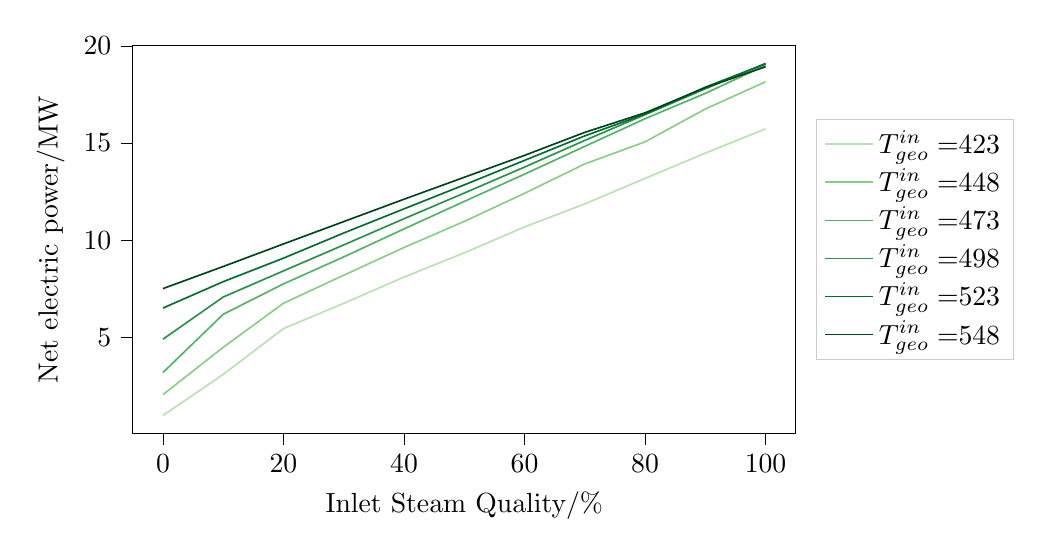
\begin{tikzpicture}

\definecolor{darkgray176}{RGB}{176,176,176}
\definecolor{darkgreen06827}{RGB}{0,68,27}
\definecolor{darkseagreen137206135}{RGB}{137,206,135}
\definecolor{forestgreen311146}{RGB}{3,111,46}
\definecolor{lightgray204}{RGB}{204,204,204}
\definecolor{mediumseagreen83179101}{RGB}{83,179,101}
\definecolor{seagreen4114674}{RGB}{41,146,74}
\definecolor{silver184226177}{RGB}{184,226,177}

\begin{axis}[
legend cell align={left},
legend style={
  fill opacity=0.8,
  draw opacity=1,
  text opacity=1,
  at={(1.03,0.5)},
  anchor=west,
  draw=lightgray204
},
tick align=outside,
tick pos=left,
x grid style={darkgray176},
xlabel={Inlet Steam Quality/\%},
xmin=-5, xmax=105,
xtick style={color=black},
y grid style={darkgray176},
ylabel={Net electric power/MW},
ymin=0.0920045033005894, ymax=20.0003393789243,
ytick style={color=black},
width=10cm, height=6.5cm
]
\addplot [semithick, silver184226177]
table {%
0 0.996928815828938
10 3.11058833145425
20 5.46557782830719
30 6.76140309847463
40 8.11093311520466
50 9.35682719969268
60 10.6869402494694
70 11.8743304888068
80 13.1830309885614
90 14.4827119441876
100 15.7342034289621
};
\addlegendentry{\(T_{geo}^{in}=\)\qty{423}{\K}}
\addplot [semithick, darkseagreen137206135]
table {%
0 2.06915745116888
10 4.50223017746847
20 6.76790514393831
30 8.208067191828
40 9.6316961427017
50 10.9726043914408
60 12.4176998239804
70 13.9291544365588
80 15.0637670570443
90 16.7527035446637
100 18.1500871993978
};
\addlegendentry{\(T_{geo}^{in}=\)\qty{448}{\K}}
\addplot [semithick, mediumseagreen83179101]
table {%
0 3.20582250186082
10 6.19997990798818
20 7.7614623276642
30 9.14922427565124
40 10.5871295071888
50 12.000787287588
60 13.4035441691335
70 14.8305129464694
80 16.2528658444977
90 17.5542142805822
100 19.0023038371704
};
\addlegendentry{\(T_{geo}^{in}=\)\qty{473}{\K}}
\addplot [semithick, seagreen4114674]
table {%
0 4.91795932112408
10 7.08629915949846
20 8.42974441921597
30 9.76491221593696
40 11.1109928808856
50 12.4301793089641
60 13.7667647948044
70 15.1360127212942
80 16.4604420990036
90 17.7893267685513
100 19.0954150663959
};
\addlegendentry{\(T_{geo}^{in}=\)\qty{498}{\K}}
\addplot [semithick, forestgreen311146]
table {%
0 6.51869778418778
10 7.87581049957509
20 9.08463379407769
30 10.3775023462663
40 11.6189613334952
50 12.8510782011073
60 14.1100450572359
70 15.3695725417207
80 16.492034103703
90 17.8728343673776
100 19.0751400690423
};
\addlegendentry{\(T_{geo}^{in}=\)\qty{523}{\K}}
\addplot [semithick, darkgreen06827]
table {%
0 7.51989223310443
10 8.65572935011302
20 9.81488624874976
30 10.9642071429144
40 12.1135070433028
50 13.2414452380362
60 14.3674083893936
70 15.5509312316087
80 16.5541893435885
90 17.8479699155465
100 18.9241703814868
};
\addlegendentry{\(T_{geo}^{in}=\)\qty{548}{\K}}
\end{axis}

\end{tikzpicture}

        \caption[The net electrical power for a binary \ac{ORC} using IsoPentane as the working fluid.]{The net electrical power for a binary \ac{ORC} using IsoPentane as the working fluid as a function of inlet steam quality at different inlet temperatures.}
        \label{fig:prosim_purewater_isopentane_by_temp}
    \end{figure}

    As can be seen in Figure~\ref{fig:prosim_purewater_isopentane_by_temp}, the dependency of the net power on the geofluid inlet steam quality follows two distinct slopes, which can be attributed to a shift in the location of the pinch-point from the outlet of the pre-heater (on the working fluid side) to its inlet, Figure~\ref{fig:prosim_purewater_isopentane_TQ_by_Q}. 
    
    Considering a binary \ac{ORC} using Isopentane as the working fluid, for saturated liquid geofluids (i.e. \(x_{geo}^{in}=\)\qty{0}{\percent}) the pinch-point is located at the pre-heater outlet (on the working fluid side). The cycle parameters (i.e. \(P_{max}\) and \(\Delta T_{sh}\)) are chosen such that the cycle net power is optimised. For two-phase geofluids with small inlet steam qualities, the additional heat content of the steam, allows the pinch-point to occur at a higher temperature (and in turn maximum cycle pressure \(P_{max}\)). Once the maximum cycle pressure is reached, for any higher geofluid inlet qualities, the pinch-point is then pushed inside the pre-heater, and the cycle power can now only be maximised by raising the degree of super-heating \(\Delta T_{sh}\). For high enough steam qualities (in this case about \qty{20}{\percent}), the pinch-point is located at the pre-heater inlet (on the working fluid side. Up until this point, the increase in cycle power is driven by 1) the increase in heat flow entering the plant, thus increasing the working fluid mass rate and 2) increasingly favourable operating parameters for the \ac{ORC}. 
    
    At even higher geofluid inlet steam qualities, the cycle operating parameters remain unchanged, either because they have reached their upper bound or because the optimum parameters with respect to the source temperature have been determined. As such, the subsequent increase in net power with geofluid inlet steam quality are now simply a result of the increased heat flow.

    \begin{figure}[H]
        \centering
        \input{Content/ProSim/Thermo_Comp/Plots/00_SimpleORC_higher_def/Isopentane_TQs_by_Q}
        \caption[TQ diagrams for a binary \ac{ORC} using Isopentane as the working fluid by steam quality.]{Temperature-Heat transferred diagrams for a binary \ac{ORC} using Isopentane as the working fluid for different geofluid steam qualities.}
        \label{fig:prosim_purewater_isopentane_TQ_by_Q}
    \end{figure}        

    At even higher geofluid inlet steam qualities, the cycle operating parameters remain unchanged, either because they have reached their upper bound or because the optimum parameters with respect to the source temperature have been determined. As such, the subsequent increase in net power with geofluid inlet steam quality are now simply a result of the increased heat flow.

    A similar behaviour can also be observed with respect to the geofluid inlet temperature, where for higher geofluid inlet temperatures, the pinch-point shifts towards the pre-heater inlet (on the working fluid side), Figure~\ref{fig:prosim_purewater_isopentane_TQ_by_T}

    \begin{figure}[H]
        \centering
        \input{Content/ProSim/Thermo_Comp/Plots/00_SimpleORC_higher_def/Isopentane_TQs_by_T}
        \caption[TQ diagrams for a binary \ac{ORC} using Isopentane as the working fluid by inlet temperature.]{Temperature-Heat transferred diagrams for a binary \ac{ORC} using Isopentane as the working fluid for different geofluid inlet temperatures.}
        \label{fig:prosim_purewater_isopentane_TQ_by_T}
    \end{figure}

    Regarding the optimisation of process variables, the following trends can be identified:

    \begin{itemize}
        \item The reduced pressure \(P_r\) increases with both geofluid inlet temperature and pressure as a result of the pinch-point shifting towards the pre-heater inlet, Figure~\ref{fig:prosim_purewater_isopentane_Pr}.

        \begin{figure}[H]
            \centering
            % This file was created with tikzplotlib v0.10.1.
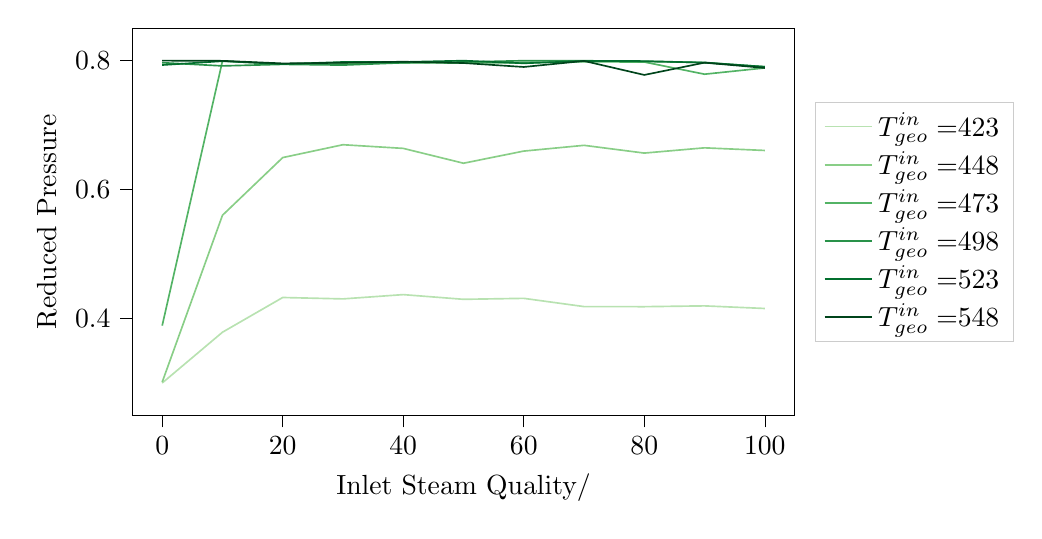
\begin{tikzpicture}

\definecolor{darkgray176}{RGB}{176,176,176}
\definecolor{darkgreen06827}{RGB}{0,68,27}
\definecolor{darkseagreen137206135}{RGB}{137,206,135}
\definecolor{forestgreen311146}{RGB}{3,111,46}
\definecolor{lightgray204}{RGB}{204,204,204}
\definecolor{mediumseagreen83179101}{RGB}{83,179,101}
\definecolor{seagreen4114674}{RGB}{41,146,74}
\definecolor{silver184226177}{RGB}{184,226,177}

\begin{axis}[
legend cell align={left},
legend style={
  fill opacity=0.8,
  draw opacity=1,
  text opacity=1,
  at={(1.03,0.5)},
  anchor=west,
  draw=lightgray204
},
tick align=outside,
tick pos=left,
x grid style={darkgray176},
xlabel={Inlet Steam Quality/\unit{\percent}},
xmin=-5, xmax=105,
xtick style={color=black},
y grid style={darkgray176},
ylabel={Reduced Pressure},
ymin=0.25, ymax=0.85,
ytick style={color=black},
width=10cm, height=6.5cm
]
\addplot [semithick, silver184226177]
table {%
0 0.300338998908966
10 0.378995417582669
20 0.432812302192289
30 0.430646390124058
40 0.437268634518456
50 0.429988447815741
60 0.431494372005636
70 0.418716172877991
80 0.418583858373748
90 0.419822254338872
100 0.415795788318756
};
\addlegendentry{\(T_{geo}^{in}=\)\qty{423}{\K}}
\addplot [semithick, darkseagreen137206135]
table {%
0 0.301700622227905
10 0.560169067077117
20 0.649577789361573
30 0.669499475737548
40 0.663819268934738
50 0.64084212334826
60 0.65964621215178
70 0.668557391454019
80 0.656556432213913
90 0.664681280470279
100 0.660615950846251
};
\addlegendentry{\(T_{geo}^{in}=\)\qty{448}{\K}}
\addplot [semithick, mediumseagreen83179101]
table {%
0 0.389248654268729
10 0.799184909347775
20 0.794339933629174
30 0.795348763920488
40 0.796515228692639
50 0.796108157301763
60 0.796609059402139
70 0.798010787152417
80 0.797637852149423
90 0.778777797019763
100 0.788454108024286
};
\addlegendentry{\(T_{geo}^{in}=\)\qty{473}{\K}}
\addplot [semithick, seagreen4114674]
table {%
0 0.79655946561082
10 0.791619816001734
20 0.794037569406178
30 0.792898147500602
40 0.79649446811868
50 0.797679261012402
60 0.799676507907949
70 0.799670350396366
80 0.798427829467034
90 0.796944291418998
100 0.790201679893791
};
\addlegendentry{\(T_{geo}^{in}=\)\qty{498}{\K}}
\addplot [semithick, forestgreen311146]
table {%
0 0.792970937565368
10 0.798951538284644
20 0.794456316884689
30 0.797685043430649
40 0.7976957307693
50 0.799730247997903
60 0.795643913737324
70 0.799270778064242
80 0.799079022014512
90 0.796664944928293
100 0.790325352294371
};
\addlegendentry{\(T_{geo}^{in}=\)\qty{523}{\K}}
\addplot [semithick, darkgreen06827]
table {%
0 0.799775920206272
10 0.799469519618339
20 0.795486271125095
30 0.79649446811868
40 0.798114039266387
50 0.796084332137947
60 0.789952071335059
70 0.799298824455227
80 0.777614892720135
90 0.796664944928293
100 0.788454108024286
};
\addlegendentry{\(T_{geo}^{in}=\)\qty{548}{\K}}
\end{axis}

\end{tikzpicture}

            \caption[The optimised reduced pressure \(P_r\) for a binary \ac{ORC} using Isopentane as the working fluid.]{The optimised reduced pressure \(P_r\) for a binary \ac{ORC} using Isopentane as the working fluid as a function of inlet steam quality at different inlet temperatures.}
            \label{fig:prosim_purewater_isopentane_Pr}
        \end{figure}
        
        \item The minimum temperature \(T_{min}\) is virtually independent of the geofluid inlet temperature and steam quality, Figure~\ref{fig:prosim_purewater_isopentane_TminTmax}, and assumes values close to the specified lower bound value of \qty{303}{\K} (\qty{30}{\degreeCelsius}). As such, the condensation pressure for each working fluid is essentially fixed for all geofluid inlet conditions and may therefore be omitted as an optimisation variable. Instead, the minimum cycle temperature \(T_{min}\), could be estimated based on the ambient temperature \(T_{amb}\) and the minimum approach temperature in the condenser \(\Delta T_{cond}^{min}\).

        \begin{figure}[H]
            \centering
            % This file was created with tikzplotlib v0.10.1.
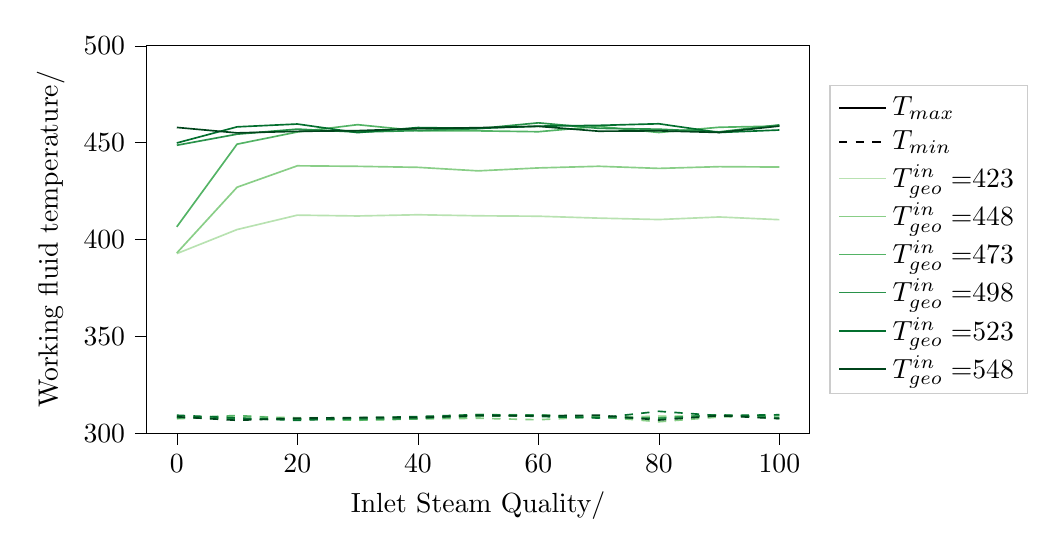
\begin{tikzpicture}

\definecolor{darkgray176}{RGB}{176,176,176}
\definecolor{darkgreen06827}{RGB}{0,68,27}
\definecolor{darkseagreen137206135}{RGB}{137,206,135}
\definecolor{forestgreen311146}{RGB}{3,111,46}
\definecolor{lightgray204}{RGB}{204,204,204}
\definecolor{mediumseagreen83179101}{RGB}{83,179,101}
\definecolor{seagreen4114674}{RGB}{41,146,74}
\definecolor{silver184226177}{RGB}{184,226,177}

\begin{axis}[
legend cell align={left},
legend style={
  fill opacity=0.8,
  draw opacity=1,
  text opacity=1,
  at={(1.03,0.5)},
  anchor=west,
  draw=lightgray204
},
tick align=outside,
tick pos=left,
x grid style={darkgray176},
xlabel={Inlet Steam Quality/\unit{\percent}},
xmin=-5, xmax=105,
xtick style={color=black},
y grid style={darkgray176},
ylabel={Working fluid temperature/\unit{\K}},
ymin=300, ymax=500,
ytick style={color=black},
width=10cm, height=6.5cm
]
\addplot [semithick, black]
table {%
0 273
1 273
};
\addlegendentry{\(T_{max}\)}
\addplot [semithick, black, dashed]
table {%
0 273
1 273
};
\addlegendentry{\(T_{min}\)}
\addplot [semithick, silver184226177]
table {%
0 392.683028606844
10 405.106748686668
20 412.548950415348
30 412.124641900786
40 412.752708583283
50 412.221458337194
60 411.994211514532
70 411.011523138382
80 410.280764089709
90 411.604231935841
100 410.211288811167
};
\addlegendentry{\(T_{geo}^{in}=\)\qty{423}{\K}}
\addplot [semithick, darkseagreen137206135]
table {%
0 392.997306377288
10 426.967382597129
20 438.028674061724
30 437.76264661153
40 437.240736069498
50 435.419171230334
60 436.935641522517
70 437.78903267515
80 436.693202630144
90 437.592611247219
100 437.389060189307
};
\addlegendentry{\(T_{geo}^{in}=\)\qty{448}{\K}}
\addplot [semithick, mediumseagreen83179101]
table {%
0 406.530837412821
10 449.209886882464
20 455.492245361728
30 459.268347787927
40 456.169519211034
50 456.068946123952
60 455.628775390454
70 458.369772696946
80 455.237971067129
90 457.93507950534
100 458.557204900285
};
\addlegendentry{\(T_{geo}^{in}=\)\qty{473}{\K}}
\addplot [semithick, seagreen4114674]
table {%
0 448.644518389569
10 454.36432258145
20 456.975410959116
30 455.456556843315
40 456.222600169204
50 457.226502864521
60 460.216594183369
70 457.389892330748
80 456.933909190057
90 455.548034125113
100 459.171526936686
};
\addlegendentry{\(T_{geo}^{in}=\)\qty{498}{\K}}
\addplot [semithick, forestgreen311146]
table {%
0 449.826311890658
10 458.144141265068
20 459.604859572225
30 455.16774274565
40 457.781936849657
50 457.343138247923
60 458.505611028065
70 458.901090798296
80 459.733889422291
90 455.251141619798
100 456.51313946343
};
\addlegendentry{\(T_{geo}^{in}=\)\qty{523}{\K}}
\addplot [semithick, darkgreen06827]
table {%
0 457.845682330817
10 455.025467795955
20 455.82493614095
30 456.186007697846
40 457.22380340233
50 457.714003086593
60 458.405480563938
70 455.899252975323
80 456.093429767371
90 455.251141619798
100 458.557204900285
};
\addlegendentry{\(T_{geo}^{in}=\)\qty{548}{\K}}
\addplot [semithick, silver184226177, dashed, forget plot]
table {%
0 307.274392731185
10 308.787642333499
20 307.964636173449
30 307.754706703285
40 308.198675050012
50 309.643958933097
60 309.368708143228
70 308.099983400492
80 308.813906081799
90 308.928606769924
100 309.357186184384
};
\addplot [semithick, darkseagreen137206135, dashed, forget plot]
table {%
0 308.948430904111
10 307.722355851882
20 307.279991441864
30 306.638201312088
40 307.301067205274
50 307.648971376968
60 306.88712446077
70 308.480219823182
80 305.843330676772
90 308.315114217303
100 309.125195108615
};
\addplot [semithick, mediumseagreen83179101, dashed, forget plot]
table {%
0 307.748878101654
10 309.084880478159
20 307.273056407061
30 306.737080665534
40 307.433277009679
50 308.577053921001
60 309.242021990555
70 308.537190713157
80 307.964525076868
90 309.376733498304
100 307.476691902325
};
\addplot [semithick, seagreen4114674, dashed, forget plot]
table {%
0 308.095106234119
10 307.231846026009
20 307.133420208092
30 307.265762066347
40 307.494475051292
50 309.397242862393
60 309.356759813683
70 307.980297273959
80 307.586430540329
90 309.459359835631
100 308.036548579989
};
\addplot [semithick, forestgreen311146, dashed, forget plot]
table {%
0 309.209965743579
10 307.792803049655
20 306.574683151019
30 307.817262505918
40 308.505085850467
50 309.547738182962
60 308.603535553553
70 307.787203031096
80 311.249288502868
90 308.996098086154
100 309.455500855707
};
\addplot [semithick, darkgreen06827, dashed, forget plot]
table {%
0 308.4209661978
10 306.58702840077
20 307.705658598355
30 308.019579765881
40 308.008357718843
50 309.023949583397
60 308.890132052346
70 309.238940050966
80 306.747052660442
90 308.996098086154
100 307.476691902325
};
\end{axis}

\end{tikzpicture}

            \caption[The minimum cycle temperature \(T_{min}\) and the maximum cycle temperatures \(T_{max}\) for a binary \ac{ORC} using Isopentane as the working fluid.]{The minimum cycle temperature \(T_{min}\) and the maximum cycle temperatures \(T_{max}\) for a binary \ac{ORC} using Isopentane as the working fluid as a function of inlet steam quality at different inlet temperatures.}
            \label{fig:prosim_purewater_isopentane_TminTmax}
        \end{figure}

        \item The degree of super-heating \(\Delta T_{sh}\) generally only begins to increase once the maximum cycle temperature can no longer be increased by raising the reduced pressure \(P_r\), Figure~\ref{fig:prosim_purewater_isopentane_DTsh}.

        \begin{figure}[H]
            \centering
            % This file was created with tikzplotlib v0.10.1.
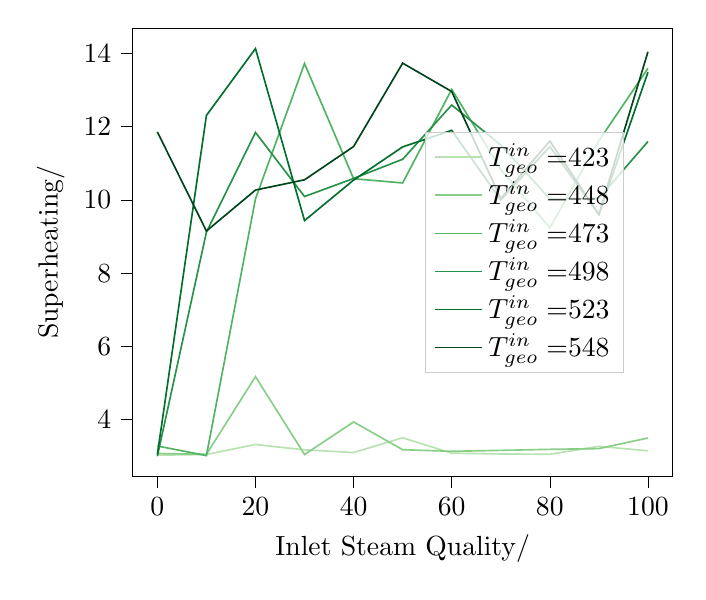
\begin{tikzpicture}

\definecolor{darkgray176}{RGB}{176,176,176}
\definecolor{darkgreen06827}{RGB}{0,68,27}
\definecolor{darkseagreen137206135}{RGB}{137,206,135}
\definecolor{forestgreen311146}{RGB}{3,111,46}
\definecolor{lightgray204}{RGB}{204,204,204}
\definecolor{mediumseagreen83179101}{RGB}{83,179,101}
\definecolor{seagreen4114674}{RGB}{41,146,74}
\definecolor{silver184226177}{RGB}{184,226,177}

\begin{axis}[
legend cell align={left},
legend style={
  fill opacity=0.8,
  draw opacity=1,
  text opacity=1,
  at={(0.91,0.5)},
  anchor=east,
  draw=lightgray204
},
tick align=outside,
tick pos=left,
x grid style={darkgray176},
xlabel={Inlet Steam Quality/\unit{\percent}},
xmin=-5, xmax=105,
xtick style={color=black},
y grid style={darkgray176},
ylabel={Superheating/\unit{\K}},
ymin=2.44836194923737, ymax=14.6905336373335,
ytick style={color=black}
]
\addplot [semithick, silver184226177]
table {%
0 3.03255147384084
10 3.04989975693593
20 3.32365093059053
30 3.17780611939241
40 3.10338376923193
50 3.50759502715692
60 3.0858798447436
70 3.06528689107108
80 3.05640285627334
90 3.2728406555234
100 3.15111495791228
};
\addlegendentry{\(T_{geo}^{in}=\)\qty{423}{\K}}
\addplot [semithick, darkseagreen137206135]
table {%
0 3.07726771656274
10 3.05439804289551
20 5.17619667388823
30 3.04981613014303
40 3.93895767799694
50 3.18143260842862
60 3.13744033465753
70 3.16319260346307
80 3.19093430376813
90 3.21166322534577
100 3.50036948389373
};
\addlegendentry{\(T_{geo}^{in}=\)\qty{448}{\K}}
\addplot [semithick, mediumseagreen83179101]
table {%
0 3.28202033542709
10 3.02086172912459
20 10.0308147906924
30 13.7258408326094
40 10.5803747542313
50 10.465465686841
60 13.0217403330603
70 10.8348847009139
80 9.23726117683225
90 11.6179067123497
100 13.5938237784206
};
\addlegendentry{\(T_{geo}^{in}=\)\qty{473}{\K}}
\addplot [semithick, seagreen4114674]
table {%
0 3.00482429869629
10 9.12192663039394
20 11.8439792388323
30 10.0946062697594
40 10.5881205202329
50 11.1123042252462
60 12.5931618854648
70 11.5010405812411
80 10.0300959511133
90 10.0502699280686
100 11.5958312913974
};
\addlegendentry{\(T_{geo}^{in}=\)\qty{498}{\K}}
\addplot [semithick, forestgreen311146]
table {%
0 3.05063190889007
10 12.3085263604075
20 14.1340712878746
30 9.43780506863891
40 10.5444988484767
50 11.449497109823
60 11.9017831853617
70 9.99915489322495
80 11.4591088560492
90 9.60298617596192
100 13.4891216813468
};
\addlegendentry{\(T_{geo}^{in}=\)\qty{523}{\K}}
\addplot [semithick, darkgreen06827]
table {%
0 11.8594046646244
10 9.15267658268192
20 10.271384814248
30 10.5515280488742
40 11.4594987849496
50 13.7367012508931
60 12.9628115921322
70 10.0401149870127
80 11.6105435645221
90 9.60298617596192
100 14.0472551702903
};
\addlegendentry{\(T_{geo}^{in}=\)\qty{548}{\K}}
\end{axis}

\end{tikzpicture}

            \caption[The degrees of super-heating \(\Delta T_{sh}\) for a binary \ac{ORC} using Isopentane.]{The degrees of super-heating \(\Delta T_{sh}\) for a binary \ac{ORC} using Isopentane as the working fluid as a function of inlet steam quality at different inlet temperatures.}
            \label{fig:prosim_purewater_isopentane_DTsh}
        \end{figure}

    \end{itemize}

    The \emph{noisiness} of the optimisation variables (e.g. the degrees of super-heating) with respect to the geofluid inlet conditions, can be attributed to degeneracy of the optimisation problem. As such there may be multiple (or even infinite) combinations of the optimisation variables that yield the same value (or similar values) of the objective function. 
    
    For example, considering a binary \ac{ORC} using IsoPentane as the working fluid, operating on a geofluid inlet temperature of \qty{473}{\K} (\qty{200}{\degreeCelsius}) and steam quality of \qty{20}{\percent}, the normalised objective function (i.e. \(\frac{W_{net,\;elec}}{W_{net,\;elec}^{max}}\)) was calculated for the full range of optimisation variables (i.e. \(P_r\) and \(DT_{sh}\)). For simplicity, the minimum cycle temperature \(T_{min}\) was fixed at \qty{308}{\K} (\qty{35}{\degreeCelsius}), Figure~\ref{fig:prosim_purewater_isopentane_objFunc_shape}.

    As can be seen from Figure~\ref{fig:prosim_purewater_isopentane_objFunc_shape}, there are many combinations of the reduced pressure \(P_r\) and the degrees of super-heating \(\Delta T_{sh}\) that yield a normalised objective function value of \num{0.99}. Nevertheless, the optimisation has converged satisfactorily (i.e. the average value of the objective function across all \emph{species} is within \qty{1}{\percent} of the best \emph{species} encountered, Figure~\ref{fig:prosim_purewater_isopentane_objFunc_Convergence}. In principle the \emph{noisiness} could be reduced by lowering the convergence tolerance for the optimisation (set at \qty{1}{\percent} for this study), however this comes at the expense of increased model runtime, however even with the default tolerance, the optimisation comes within \qty{0.1}{\percent} of the global optimum value of the objective function as determined via the brute-force approach.

    \begin{figure}[H]
        \centering
        \input{Content/ProSim/Thermo_Comp/Plots/00_SimpleORC/ObjFuncShape}
        \caption[The normalised objective function space for a binary \ac{ORC} using IsoPentane as the working fluid.]{The normalised objective function space (i.e. \(\frac{W_{net,\;elec}}{W_{net,\;elec}^{max}}\)) for a binary \ac{ORC} using IsoPentane as the working fluid, operating on a geofluid temperature of \qty{473}{\K} (\qty{200}{\degreeCelsius}) and steam quality of \qty{20}{\percent}. The minimum cycle temperature \(T_{min}\) is fixed at \qty{308}{\K} (\qty{35}{\degreeCelsius}). The black star indicates the global optimum point; the black circle indicates the optimum operating conditions found in \emph{PowerCycle}.}
        \label{fig:prosim_purewater_isopentane_objFunc_shape}
    \end{figure}

    \begin{figure}[H]
        \centering
        \input{Content/ProSim/Thermo_Comp/Plots/00_SimpleORC/ObjFuncConvergence}
        \caption[The normalised objective function convergence for a binary \ac{ORC} using IsoPentane as the working fluid.]{The normalised objective function (i.e. \(\frac{W_{net,\;elec}}{W_{net,\;elec}^{max}}\)) as a function of the optimiser iterations for a binary \ac{ORC} using IsoPentane as the working fluid, operating on a geofluid temperature of \qty{473}{\K} (\qty{200}{\degreeCelsius}) and steam quality of \qty{20}{\percent}. The minimum cycle temperature \(T_{min}\) is fixed at \qty{308}{\K} (\qty{35}{\degreeCelsius}). The black star indicates the global optimum point; the black circle indicates the optimum operating conditions found in \emph{PowerCycle}.}
        \label{fig:prosim_purewater_isopentane_objFunc_Convergence}
    \end{figure}

    \begin{figure}[H]
        \centering
        % This file was created with tikzplotlib v0.10.1.
\begin{tikzpicture}

\definecolor{crimson2143940}{RGB}{214,39,40}
\definecolor{darkgray176}{RGB}{176,176,176}
\definecolor{darkorange25512714}{RGB}{255,127,14}
\definecolor{forestgreen4416044}{RGB}{44,160,44}
\definecolor{gray127}{RGB}{127,127,127}
\definecolor{lightgray204}{RGB}{204,204,204}
\definecolor{mediumpurple148103189}{RGB}{148,103,189}
\definecolor{orchid227119194}{RGB}{227,119,194}
\definecolor{sienna1408675}{RGB}{140,86,75}
\definecolor{steelblue31119180}{RGB}{31,119,180}

\begin{groupplot}[
    group style={
        group size=2 by 3, 
        vertical sep=2.5cm, 
        horizontal sep=2cm},
    height=6cm, 
    width=7cm,
    ymin=0,
    ymax=30
]
\nextgroupplot[
tick align=outside,
tick pos=left,
title={\(T_{geo}^{in}=\)\qty{423}{\K}},
unbounded coords=jump,
x grid style={darkgray176},
xlabel={Inlet Steam Quality/\unit{\percent}},
xmin=-5, xmax=105,
xtick style={color=black},
y grid style={darkgray176},
ylabel={Net electric power/\unit{\mega\watt}},
% ymin=0.249722311926874, ymax=16.6916073852991,
ytick style={color=black}
]
\addplot [semithick, steelblue31119180]
table {%
0 1.23307554564229
10 2.05815064988225
20 2.71008207381181
30 3.37317976519898
40 4.02686322561301
50 4.68572554047509
60 5.33656273188152
70 5.99452273687179
80 6.66016555489133
90 7.31336965330137
100 7.92987716054522
};
\addplot [semithick, darkorange25512714]
table {%
0 1.23605473349499
10 3.09772594029469
20 4.38840529184299
30 5.46189923595034
40 6.4897661177099
50 7.58614921737735
60 8.63847561605827
70 9.70373614857271
80 10.7596993623856
90 11.8353663021898
100 12.8708089665933
};
\addplot [semithick, forestgreen4416044]
table {%
0 1.30383936970953
10 3.43578747361516
20 4.61071939495868
30 5.71555476015857
40 6.82301411139795
50 7.92598328364551
60 9.04457194969536
70 10.1576803422948
80 11.2644085561581
90 12.3755565142169
100 13.4531729451081
};
\addplot [semithick, crimson2143940]
table {%
0 1.26892558049531
10 3.57560728887553
20 5.23704673458202
30 6.47128718827251
40 7.72845748287371
50 9.0180983307172
60 10.2716770649003
70 11.5255850010607
80 12.7270348488864
90 14.0169076020581
100 15.3300887365762
};
\addplot [semithick, mediumpurple148103189]
table {%
0 0.997080724352886
10 3.11247857630618
20 5.4661107357926
30 6.76528969957147
40 8.11107101643414
50 9.37305147896936
60 10.6932339061055
70 12.0184774258505
80 13.1831280972173
90 14.6036011158268
100 15.9442489728731
};
\addplot [semithick, sienna1408675]
table {%
0 nan
10 nan
20 nan
30 nan
40 nan
50 nan
60 nan
70 nan
80 nan
90 nan
100 nan
};
\addplot [semithick, orchid227119194]
table {%
0 nan
10 nan
20 nan
30 nan
40 nan
50 nan
60 nan
70 nan
80 nan
90 nan
100 nan
};
\addplot [semithick, gray127]
table {%
0 nan
10 nan
20 nan
30 nan
40 nan
50 nan
60 nan
70 nan
80 nan
90 nan
100 nan
};
\addplot [very thick, black, dotted]
table {%
0 1.30383936970953
10 3.57560728887553
20 5.4661107357926
30 6.76528969957147
40 8.11107101643414
50 9.37305147896936
60 10.6932339061055
70 12.0184774258505
80 13.1831280972173
90 14.6036011158268
100 15.9442489728731
};

\nextgroupplot[
tick align=outside,
tick pos=left,
title={\(T_{geo}^{in}=\)\qty{448}{\K}},
unbounded coords=jump,
x grid style={darkgray176},
xlabel={Inlet Steam Quality/\unit{\percent}},
xmin=-5, xmax=105,
xtick style={color=black},
y grid style={darkgray176},
ylabel={Net electric power/\unit{\mega\watt}},
% ymin=-0.603621914129284, ymax=21.9976318404959,
ytick style={color=black}
]
\addplot [semithick, steelblue31119180]
table {%
0 1.74044380449781
10 2.3679970423708
20 3.00304723513269
30 3.63586311110214
40 4.26733960838878
50 4.89176595320707
60 5.52902977727053
70 6.16243761324868
80 6.78477081687379
90 7.42503823061354
100 8.04869483009499
};
\addplot [semithick, darkorange25512714]
table {%
0 2.18417660227125
10 3.80858746550322
20 4.8484937672049
30 5.88301980081586
40 6.89621118590216
50 7.91626850527473
60 8.92870605645356
70 9.97199176870959
80 11.0162329668643
90 12.0029026692291
100 13.041015769229
};
\addplot [semithick, forestgreen4416044]
table {%
0 2.43235913934194
10 4.02253638350673
20 5.08668865792427
30 6.15419445905022
40 7.19661763614806
50 8.27688117447675
60 9.32211695261562
70 10.4187577457176
80 11.4887629559207
90 12.5349485627673
100 13.5919942860922
};
\addplot [semithick, crimson2143940]
table {%
0 2.19190926377515
10 4.64737177870475
20 5.95606611316397
30 7.20175010897739
40 8.45050815445731
50 9.6917614241624
60 10.8923606719033
70 12.1802896588927
80 13.4370912870964
90 14.6910491419213
100 15.9627685659099
};
\addplot [semithick, mediumpurple148103189]
table {%
0 2.06984836523573
10 4.50262146929036
20 6.76808706370316
30 8.21366092030203
40 9.63243065593898
50 10.9750629359449
60 12.4189373032357
70 13.9294211595266
80 15.2157970005596
90 16.7792938304432
100 18.1562041420369
};
\addplot [semithick, sienna1408675]
table {%
0 0.971115623399739
10 4.05951316868544
20 6.85632563895486
30 8.25863624951761
40 9.65506686829158
50 11.3168135267237
60 12.7164190632256
70 14.1979101956436
80 15.3979217619467
90 16.7674424792211
100 18.2138658663401
};
\addplot [semithick, orchid227119194]
table {%
0 0.423707801990044
10 3.67193133589524
20 6.8039035955362
30 9.4842162356594
40 11.1434320567881
50 12.7814962389121
60 14.414929485041
70 16.050822588424
80 17.6868807451047
90 19.3298281437926
100 20.9703021243766
};
\addplot [semithick, gray127]
table {%
0 nan
10 nan
20 nan
30 nan
40 nan
50 nan
60 nan
70 nan
80 nan
90 nan
100 nan
};
\addplot [very thick, black, dotted]
table {%
0 2.43235913934194
10 4.64737177870475
20 6.85632563895486
30 9.4842162356594
40 11.1434320567881
50 12.7814962389121
60 14.414929485041
70 16.050822588424
80 17.6868807451047
90 19.3298281437926
100 20.9703021243766
};

\nextgroupplot[
tick align=outside,
tick pos=left,
title={\(T_{geo}^{in}=\)\qty{473}{\K}},
unbounded coords=jump,
x grid style={darkgray176},
xlabel={Inlet Steam Quality/\unit{\percent}},
xmin=-5, xmax=105,
xtick style={color=black},
y grid style={darkgray176},
ylabel={Net electric power/\unit{\mega\watt}},
% ymin=1.0316404306704, ymax=24.1600227299206,
ytick style={color=black}
]
\addplot [semithick, steelblue31119180]
table {%
0 2.08293053518177
10 2.68021051917038
20 3.29139380829806
30 3.88995077267013
40 4.4949840309543
50 5.09495606783933
60 5.69258822474231
70 6.26701417625023
80 6.89048949521264
90 7.50373845006295
100 8.10183027573824
};
\addplot [semithick, darkorange25512714]
table {%
0 3.18050884619529
10 4.34442460968987
20 5.31974952052081
30 6.28674698495501
40 7.27855962178412
50 8.25479724082798
60 9.23878936820798
70 10.2211822653079
80 11.1795045291975
90 12.157092502791
100 13.1399915533479
};
\addplot [semithick, forestgreen4416044]
table {%
0 3.48387222154788
10 4.55810651647044
20 5.55691956390842
30 6.59185721295109
40 7.61157637142634
50 8.62651868541596
60 9.64828309505694
70 10.6622234405878
80 11.6875118150123
90 12.7043603681735
100 13.7318381314814
};
\addplot [semithick, crimson2143940]
table {%
0 3.75045845803565
10 5.3233703834005
20 6.52143371948183
30 7.72325173820614
40 8.90734085878473
50 10.0900882744869
60 11.2859816404378
70 12.4799494051229
80 13.6582927603245
90 14.8580333710726
100 16.0578783341456
};
\addplot [semithick, mediumpurple148103189]
table {%
0 3.20582250186064
10 6.20864419417077
20 7.77026521865386
30 9.15793721359779
40 10.5942558910995
50 12.0016291313923
60 13.4131519723005
70 14.8333281654913
80 16.2534795641855
90 17.5885050963295
100 19.0062543011339
};
\addplot [semithick, sienna1408675]
table {%
0 2.66390898999459
10 5.58764839607512
20 8.20326772106154
30 9.52415154429392
40 10.8759656629603
50 12.7047094653499
60 14.0275429276572
70 15.7691999870244
80 17.2234139111199
90 18.7308158836152
100 20.1875507563209
};
\addplot [semithick, orchid227119194]
table {%
0 2.19758099329316
10 5.23652585332202
20 8.67312917722763
30 11.0935064407358
40 12.8214828457216
50 14.4968444963231
60 16.2755538019646
70 17.9171619822363
80 19.7341420230545
90 21.4724684505193
100 23.1087326254092
};
\addplot [semithick, gray127]
table {%
0 nan
10 nan
20 nan
30 nan
40 nan
50 nan
60 nan
70 nan
80 nan
90 nan
100 nan
};
\addplot [very thick, black, dotted]
table {%
0 3.75045845803565
10 6.20864419417077
20 8.67312917722763
30 11.0935064407358
40 12.8214828457216
50 14.4968444963231
60 16.2755538019646
70 17.9171619822363
80 19.7341420230545
90 21.4724684505193
100 23.1087326254092
};

\nextgroupplot[
tick align=outside,
tick pos=left,
title={\(T_{geo}^{in}=\)\qty{498}{\K}},
x grid style={darkgray176},
xlabel={Inlet Steam Quality/\unit{\percent}},
xmin=-5, xmax=105,
xtick style={color=black},
y grid style={darkgray176},
ylabel={Net electric power/\unit{\mega\watt}},
% ymin=1.32292057843257, ymax=25.7920105582779,
ytick style={color=black}
]
\addplot [semithick, steelblue31119180]
table {%
0 2.43515194115281
10 3.0074878400552
20 3.57889969384682
30 4.15009748891496
40 4.71459711608513
50 5.27807478627922
60 5.85701131088781
70 6.41435196343493
80 7.00545026663586
90 7.57119632014405
100 8.13727110182161
};
\addplot [semithick, darkorange25512714]
table {%
0 3.91328722366362
10 4.8557129366323
20 5.78773150015289
30 6.70102643826149
40 7.62514915278658
50 8.57511413979024
60 9.4855235606839
70 10.3574896359272
80 11.3560957385295
90 12.2357884666063
100 13.1576506285015
};
\addplot [semithick, forestgreen4416044]
table {%
0 4.13400807449359
10 5.09484745877595
20 6.04834955640886
30 7.02296950633189
40 7.98103177861806
50 8.94850028875134
60 9.90111359237432
70 10.8564064607697
80 11.8097606026707
90 12.8069565408167
100 13.7626444981277
};
\addplot [semithick, crimson2143940]
table {%
0 4.80339701119734
10 5.96167414778723
20 7.08860788743319
30 8.22014410954733
40 9.34712087668993
50 10.470895671257
60 11.6094636572213
70 12.7332688105737
80 13.8550959632204
90 14.9815179684642
100 16.1238187732441
};
\addplot [semithick, mediumpurple148103189]
table {%
0 4.91836536741632
10 7.08665384060379
20 8.43363490574898
30 9.7686182632356
40 11.1121946281129
50 12.4312961855516
60 13.7751722398373
70 15.1360297718138
80 16.4710949067942
90 17.8198968055177
100 19.1328357287923
};
\addplot [semithick, sienna1408675]
table {%
0 4.38257730595009
10 7.59080808732406
20 9.43539933958951
30 10.9378142168666
40 12.4462939692142
50 13.9582547675079
60 15.4444469355154
70 16.9305695954869
80 18.3676208006646
90 19.9100104699709
100 21.3607695637703
};
\addplot [semithick, orchid227119194]
table {%
0 4.01115250570606
10 6.89451930154602
20 10.5703119236632
30 12.6288049426315
40 14.3877520929666
50 15.992178274343
60 17.5854937896778
70 19.392511447984
80 21.2100022069709
90 23.1240239921779
100 24.6797791955576
};
\addplot [semithick, gray127]
table {%
0 2.53658566704817
10 6.51318334331483
20 9.77471386852545
30 11.3443650376048
40 12.8818712285688
50 14.5057530989909
60 15.8578752607341
70 17.4818665806058
80 19.0793419439125
90 20.8521788290564
100 22.336590936633
};
\addplot [very thick, black, dotted]
table {%
0 4.91836536741632
10 7.59080808732406
20 10.5703119236632
30 12.6288049426315
40 14.3877520929666
50 15.992178274343
60 17.5854937896778
70 19.392511447984
80 21.2100022069709
90 23.1240239921779
100 24.6797791955576
};

\nextgroupplot[
tick align=outside,
tick pos=left,
title={\(T_{geo}^{in}=\)\qty{523}{\K}},
x grid style={darkgray176},
xlabel={Inlet Steam Quality/\unit{\percent}},
xmin=-5, xmax=105,
xtick style={color=black},
y grid style={darkgray176},
ylabel={Net electric power/\unit{\mega\watt}},
% ymin=1.659500996677, ymax=26.7615302078282,
ytick style={color=black}
]
\addplot [semithick, steelblue31119180]
table {%
0 2.80050232445661
10 3.33672770345504
20 3.86717590842396
30 4.39871815695255
40 4.92553194411864
50 5.46790312886749
60 5.99953076905021
70 6.47176067380605
80 7.04751284776612
90 7.57517997000357
100 8.12961056388782
};
\addplot [semithick, darkorange25512714]
table {%
0 4.51636812399582
10 5.38557162087143
20 6.24740997416727
30 7.09865809143434
40 7.98259140472522
50 8.86818804009482
60 9.73082712545302
70 10.5749942779788
80 11.4485397084628
90 12.2443972823418
100 13.1452620276055
};
\addplot [semithick, forestgreen4416044]
table {%
0 4.75623063709061
10 5.65012957274326
20 6.55723645455799
30 7.44333687793577
40 8.35893958659411
50 9.25184548605669
60 10.1497473204996
70 11.0071508746171
80 11.9398994519688
90 12.8521688345108
100 13.747282036225
};
\addplot [semithick, crimson2143940]
table {%
0 5.56624744040748
10 6.61781825102417
20 7.675231881771
30 8.71559081277125
40 9.75364620342651
50 10.8054575132135
60 11.8875343731025
70 12.9449823291906
80 13.9996307249257
90 15.0346834885723
100 16.1046299223092
};
\addplot [semithick, mediumpurple148103189]
table {%
0 6.53105227469323
10 7.87688511535702
20 9.09292638514086
30 10.3780177105548
40 11.6287945891221
50 12.851078204806
60 14.1239950057462
70 15.3698511721734
80 16.6070792253073
90 17.8730988329725
100 19.081941626471
};
\addplot [semithick, sienna1408675]
table {%
0 6.26479539752084
10 8.75157630419359
20 10.2264053611258
30 11.6337016735094
40 13.0244631289518
50 14.3522407393466
60 15.7415488488664
70 17.1295218423127
80 18.5044741264228
90 20.022845627633
100 21.3263100024636
};
\addplot [semithick, orchid227119194]
table {%
0 5.81671091183224
10 9.61890130932818
20 11.9702430503271
30 13.8953058038587
40 15.5939424367384
50 17.2581199254491
60 18.8143960365805
70 20.5940896671126
80 22.1619594200049
90 23.7640892261003
100 25.6205288800486
};
\addplot [semithick, gray127]
table {%
0 5.14385786490399
10 8.78384848982208
20 11.1477919046381
30 12.7168736648255
40 14.2450848181026
50 15.7465427869412
60 17.2234422789721
70 18.8021483666101
80 20.3336267356163
90 21.8625538128379
100 23.2864320685793
};
\addplot [very thick, black, dotted]
table {%
0 6.53105227469323
10 9.61890130932818
20 11.9702430503271
30 13.8953058038587
40 15.5939424367384
50 17.2581199254491
60 18.8143960365805
70 20.5940896671126
80 22.1619594200049
90 23.7640892261003
100 25.6205288800486
};

\nextgroupplot[
legend cell align={left},
legend style={fill opacity=0.8, draw opacity=1, text opacity=1, draw=lightgray204, anchor=north, at={(-0.3, -0.35)}},
legend columns=5,
tick align=outside,
tick pos=left,
title={\(T_{geo}^{in}=\)\qty{548}{\K}},
x grid style={darkgray176},
xlabel={Inlet Steam Quality/\unit{\percent}},
xmin=-5, xmax=105,
xtick style={color=black},
y grid style={darkgray176},
ylabel={Net electric power/\unit{\mega\watt}},
% ymin=2.07307940442529, ymax=26.4697708661096,
ytick style={color=black}
]
\addplot [semithick, steelblue31119180]
table {%
0 3.18201992541094
10 3.67768140811823
20 4.16655315318367
30 4.61701352510218
40 5.11926490396278
50 5.62046096181834
60 6.10689567315101
70 6.60920852938923
80 7.07784819976678
90 7.57465425889384
100 8.06798273249152
};
\addlegendentry{n-Propane}
\addplot [semithick, darkorange25512714]
table {%
0 5.14582202665663
10 5.95066627693157
20 6.72741614545184
30 7.54068487394895
40 8.33612834910577
50 9.13335774480046
60 9.90175698562114
70 10.7243236471868
80 11.4772710108401
90 12.2273585425551
100 13.0861404956773
};
\addlegendentry{CycloPropane}
\addplot [semithick, forestgreen4416044]
table {%
0 5.39089074707897
10 6.22342823199286
20 7.03550458247434
30 7.88017221186999
40 8.70506026141174
50 9.51912959842921
60 10.3534542051022
70 11.1811242890462
80 12.0141637667457
90 12.8342925300575
100 13.6755977550725
};
\addlegendentry{IsoButane}
\addplot [semithick, crimson2143940]
table {%
0 6.32348038479439
10 7.27355075494732
20 8.24488357844415
30 9.21668949583983
40 10.1917076371687
50 11.1674060360614
60 12.1275077347452
70 13.0816190503667
80 14.0395743002748
90 15.0137655256353
100 15.9998988639108
};
\addlegendentry{n-Butane}
\addplot [semithick, mediumpurple148103189]
table {%
0 7.52481264977529
10 8.65685276960452
20 9.81498883374623
30 10.9655575525893
40 12.113598271586
50 13.2440516619393
60 14.3738060330612
70 15.5510565127949
80 16.6359546608385
90 17.8482340058449
100 18.9300969842363
};
\addlegendentry{Isopentane}
\addplot [semithick, sienna1408675]
table {%
0 8.28572116340374
10 9.70115668495822
20 10.955850687072
30 12.2317182910455
40 13.5441232490194
50 14.8401099701842
60 16.1307272994057
70 17.32751091613
80 18.6438679173911
90 19.9949705612754
100 21.2902746323701
};
\addlegendentry{Isohexane}
\addplot [semithick, orchid227119194]
table {%
0 8.11701481951015
10 11.2626661490276
20 13.0758332060624
30 14.7003222648862
40 16.2513290278568
50 17.6932411667334
60 19.2969638942674
70 20.8304609730813
80 22.3119648153718
90 23.7310047679186
100 25.3608303451239
};
\addlegendentry{Cyclopentane}
\addplot [semithick, gray127]
table {%
0 7.77907269483702
10 10.4880578531455
20 12.2229811370103
30 13.646041069426
40 15.0457676183341
50 16.5062751358658
60 17.9188896157763
70 19.2844067815501
80 20.766981555164
90 22.2039901651134
100 23.6294221477471
};
\addlegendentry{n-Heptane}
\addplot [very thick, black, dotted]
table {%
0 8.28572116340374
10 11.2626661490276
20 13.0758332060624
30 14.7003222648862
40 16.2513290278568
50 17.6932411667334
60 19.2969638942674
70 20.8304609730813
80 22.3119648153718
90 23.7310047679186
100 25.3608303451239
};
\addlegendentry{Best WF}
\end{groupplot}

\end{tikzpicture}

        \caption[The net electrical power by working fluid.]{The net electrical power as a function of inlet steam quality at different inlet temperatures for a range of working fluids. The best performing working fluid is indicated by the dotted black line}
        \label{fig:prosim_purewater_wfs_by_temp}
    \end{figure}

    Comparing the performance of the different working fluids considered, Figure~\ref{fig:prosim_purewater_wfs_by_temp}, several working fluids can be seen to dominate at different geofluid inlet conditions. Overall, CycloPentane appears to be the best performing working fluid, yielding the highest net power for virtually all geofluid inlet steam qualities and temperatures greater than or equal to \qty{448}{\K}. n-Butane and Isopentane can be seen to perform well at lower temperatures and low steam qualities.

    \begin{figure}[H]
        \centering
        \input{Content/ProSim/Thermo_Comp/Plots/00_SimpleORC/Eta1stLaw}
        \caption[The 1\textsuperscript{st} law cycle, thermal recovery and plant efficiency of the binary ORC plant.]{The maximum 1\textsuperscript{st} law plant efficiency (bottom left) and corresponding cycle (top left) and thermal recovery (top right) efficiencies of the binary ORC plant across all working fluids as a function of inlet steam quality at different inlet temperatures for a range of working fluids.}
        \label{fig:prosim_purewater_eta1st_by_temp}
    \end{figure}

    The 1\textsuperscript{st} law plant efficiency for two-phase heat sources is higher than that of single-phase sources, Figure~\ref{fig:prosim_purewater_eta1st_by_temp}. The cycle efficiency increases with geofluid inlet vapour quality (up to a threshold) because the pinch point in the \ac{PHE} is shifted towards to the working fluid inlet, allowing for higher cycle temperatures. For the same reason the thermal recovery efficiency increases with geofluid inlet vapour quality, reaching values as high as \qty{97}{\percent}, irrespective of geofluid inlet temperature, for saturated vapour sources. Consequently, the plant efficiency approaches the cycle efficiency. Two-phase sources can reach plant efficiencies almost twice as high as single-phase liquid heat sources, though the effect diminished with source temperature. These trends are in keeping with what was previously identified from a theoretical perspective in section~\ref{sec:prosim_litrev_orc_efficiency}. 

    The maximum net power and the corresponding specific plant cost across all working fluids for the different geofluid inlet conditions is shown in Figure~\ref{fig:prosim_purewater_Wnet_bestWf_SpecCost}. The specific cost is compared against estimates from \emph{GEOPHIRES-X} \cite{Beckers2023}, though while the specific costs are of similar magnitude, overall agreement is poor. This could be the result of a number of factors, such as the \emph{GEOPHIRES-X} cost model being intended for at most saturated geofluids and geofluid temperatures below \qty{473}{\K}, as well as in this case the binary \ac{ORC} being optimised solely on net power.

    \begin{figure}[H]
        \centering
        % This file was created with tikzplotlib v0.10.1.
\begin{tikzpicture}

\definecolor{chocolate2369815}{RGB}{236,98,15}
\definecolor{darkgray165}{RGB}{165,165,165}
\definecolor{darkgray176}{RGB}{176,176,176}
\definecolor{darkslategray45}{RGB}{45,45,45}
\definecolor{dimgray108}{RGB}{108,108,108}
\definecolor{firebrick175572}{RGB}{175,57,2}
\definecolor{gainsboro216}{RGB}{216,216,216}
\definecolor{lightgray204}{RGB}{204,204,204}
\definecolor{lightsteelblue157201224}{RGB}{157,201,224}
\definecolor{midnightblue848107}{RGB}{8,48,107}
\definecolor{navajowhite253207161}{RGB}{253,207,161}
\definecolor{powderblue197218238}{RGB}{197,218,238}
\definecolor{saddlebrown127394}{RGB}{127,39,4}
\definecolor{sandybrown25315378}{RGB}{253,153,78}
\definecolor{sandybrown253173106}{RGB}{253,173,106}
\definecolor{silver188}{RGB}{188,188,188}
\definecolor{skyblue127184218}{RGB}{127,184,218}
\definecolor{steelblue59139194}{RGB}{59,139,194}
\definecolor{teal1287160}{RGB}{12,87,160}

\begin{groupplot}[group style={group size=1 by 2}]
\nextgroupplot[
legend cell align={left},
legend style={fill opacity=0.8, draw opacity=1, text opacity=1, draw=lightgray204},
tick align=outside,
tick pos=left,
x grid style={darkgray176},
xlabel={Inlet Steam Quality/\unit{\percent}},
xmin=-5, xmax=105,
xtick style={color=black},
y grid style={darkgray176},
ylabel={Net electric power/\unit{\mega\watt}},
ymin=0, ymax=30,
ytick style={color=black}
]
\addplot [semithick, skyblue127184218]
table {%
0 -1
1 -1
};
\addlegendentry{Binary ORC}
\addplot [semithick, chocolate2369815]
table {%
0 -1
1 -1
};
\addlegendentry{Single flash DSC}
\addplot [semithick, gainsboro216]
table {%
0 1
1 1
};
\addlegendentry{\(T_{geo}^{in}=\)\qty{423}{\K}}
\addplot [semithick, silver188]
table {%
0 1
1 1
};
\addlegendentry{\(T_{geo}^{in}=\)\qty{448}{\K}}
\addplot [semithick, darkgray165]
table {%
0 1
1 1
};
\addlegendentry{\(T_{geo}^{in}=\)\qty{473}{\K}}
\addplot [semithick, dimgray108]
table {%
0 1
1 1
};
\addlegendentry{\(T_{geo}^{in}=\)\qty{498}{\K}}
\addplot [semithick, darkslategray45]
table {%
0 1
1 1
};
\addlegendentry{\(T_{geo}^{in}=\)\qty{523}{\K}}
\addplot [semithick, black]
table {%
0 1
1 1
};
\addlegendentry{\(T_{geo}^{in}=\)\qty{548}{\K}}
\addplot [semithick, powderblue197218238, forget plot]
table {%
0 0.960849687129581
10 2.14458569253811
20 3.23035885785677
30 4.27566680248484
40 5.00700544345708
50 5.86983853781537
60 7.0594488651544
70 7.93193718867346
80 8.93664837449323
100 10.3793750090752
};
\addplot [semithick, lightsteelblue157201224, forget plot]
table {%
0 1.50952974466483
10 2.62305472157002
20 5.13252644589229
30 4.57207068080773
40 5.1310978081115
50 5.87176342204058
60 7.11533208609615
70 7.39108765599484
80 8.22080579508858
100 15.3542513774987
};
\addplot [semithick, skyblue127184218, forget plot]
table {%
0 2.09801582575957
10 3.59825615669869
20 3.89507826651621
30 4.66246522274257
40 5.48383732096798
50 6.32697641805644
60 7.05923199079413
70 8.07467669867112
80 8.93821959686381
100 10.7181908644327
};
\addplot [semithick, steelblue59139194, forget plot]
table {%
0 2.72625581513927
10 4.27047342573569
20 5.72840856540256
30 6.89239857439898
40 8.12016385080602
50 8.88948575778284
60 10.3053070490078
70 11.5409117007058
80 12.6644711957681
100 14.8640801493018
};
\addplot [semithick, teal1287160, forget plot]
table {%
0 3.40981980098837
10 4.70211364120694
20 6.01522355697679
30 7.03110269087159
40 8.1430117390292
50 9.0887040876772
60 10.2269550781848
70 11.1570874630651
80 12.1982183362838
100 14.4174746039932
};
\addplot [semithick, midnightblue848107, forget plot]
table {%
0 4.03006986002843
10 5.40480345953533
20 6.42088686926434
30 7.37991543828771
40 8.37226810980826
50 9.21659321716415
60 10.2901081894353
70 11.1013053206093
80 12.3122709020346
100 14.0852296591021
};
\addplot [semithick, navajowhite253207161, forget plot]
table {%
0 0.557114149477613
10 1.638809379093
20 3.21412473778287
30 4.88993046912543
40 6.40119018667188
50 8.01183196896339
60 9.44767830676006
70 10.8199603723257
80 12.2488536362307
100 15.2483801805043
};
\addplot [semithick, sandybrown253173106, forget plot]
table {%
0 1.08066458863151
10 2.2510134932247
20 3.92997004383771
30 5.74272006643475
40 7.49889052798885
50 9.71407527195079
60 11.2066841203576
70 13.5069457281367
80 14.7331560417993
100 18.7500172587311
};
\addplot [semithick, sandybrown25315378, forget plot]
table {%
0 1.64052050679576
10 2.87437434461262
20 4.43651027514178
30 6.54064816254777
40 8.79912360916101
50 10.7969730793877
60 12.751824036599
70 15.3704403856425
80 17.1222600178921
100 20.7412826958224
};
\addplot [semithick, chocolate2369815, forget plot]
table {%
0 2.30555058647817
10 3.65977973139912
20 4.83127169874635
30 7.24894705666434
40 9.50696724488665
50 11.9924728626009
60 13.6748087725596
70 16.757977411243
80 18.9233907014631
100 23.2626803222292
};
\addplot [semithick, firebrick175572, forget plot]
table {%
0 3.14394468871166
10 4.57715473188939
20 5.88207130807426
30 7.59483919695904
40 10.0956998814759
50 13.0154460785487
60 15.5655359107965
70 17.8582574715776
80 20.0412390531391
100 25.2823359007929
};
\addplot [semithick, saddlebrown127394, forget plot]
table {%
0 4.04694608432612
10 5.56385477936918
20 6.78431620199085
30 8.51801675553119
40 10.9574501504885
50 13.4872385647876
60 16.0443522656724
70 18.7578315602252
80 21.4234178239481
100 26.2259847001766
};
\addplot [semithick, red, mark=*, mark size=3, mark options={solid}, only marks]
table {%
20.2574810001872 3.25727355136542
25.0672234506447 4.84853098630374
15.7209666111048 3.76806709466906
27.155997056422 6.56135947321086
21.9106672040425 6.20932425141718
0 4.04694608432612
};
\addlegendentry{Break-even}

\nextgroupplot[
legend cell align={left},
legend style={fill opacity=0.8, draw opacity=1, text opacity=1, draw=lightgray204},
tick align=outside,
tick pos=left,
x grid style={darkgray176},
xlabel={Inlet Steam Quality/\unit{\percent}},
xmin=-5, xmax=105,
xtick style={color=black},
y grid style={darkgray176},
ylabel={Specific Cost/\unit{\USD\of{2023}\kilo\watt}},
ymin=0, ymax=6000,
ytick style={color=black}
]
\addplot [semithick, powderblue197218238, forget plot]
table {%
0 5019.56547982306
10 2522.57106687602
20 2240.69951062353
30 2053.98683462622
40 1941.96587910678
50 1842.47234948347
60 1780.06832167425
70 1726.41617758276
80 1686.31698562254
100 1602.83504349693
};
\addplot [semithick, lightsteelblue157201224, forget plot]
table {%
0 2744.8946588861
10 2272.38543986691
20 3348.05408810455
30 1882.88408329855
40 1771.02522520651
50 1688.72521989823
60 1631.21205136017
70 1574.09109359846
80 1533.21516140621
100 2205.44172551837
};
\addplot [semithick, skyblue127184218, forget plot]
table {%
0 2405.49149207129
10 3097.84203214475
20 1910.86221173232
30 1786.31917938869
40 1692.84297911923
50 1620.69761919165
60 1608.72937527545
70 1559.30680599622
80 1497.69192144539
100 1417.43111503078
};
\addplot [semithick, steelblue59139194, forget plot]
table {%
0 2198.3771443697
10 2622.27468624185
20 2308.61160681393
30 2113.50877997879
40 1983.50285339464
50 1884.01973590842
60 1785.66175509507
70 1723.64384618247
80 1668.84963609376
100 1569.36440336915
};
\addplot [semithick, teal1287160, forget plot]
table {%
0 2765.12486847892
10 2301.36862785584
20 2055.65553040038
30 1889.16536367077
40 1775.25384422885
50 1688.64847789024
60 1626.58498625757
70 1569.94847324597
80 1501.58429232089
100 1419.16357696616
};
\addplot [semithick, midnightblue848107, forget plot]
table {%
0 2364.49395107708
10 2082.70271598588
20 1902.65310939968
30 1778.30302161461
40 1681.76596511172
50 1605.11369334188
60 1540.95964264706
70 1487.43202350552
80 1443.68293367015
100 1365.31239325101
};
\addplot [semithick, navajowhite253207161, forget plot]
table {%
0 4888.7143335263
10 3404.0250225565
20 2765.54563623294
30 2409.1559187536
40 2183.27858115757
50 2009.69985620321
60 1878.59416928319
70 1781.0224664262
80 1687.7740515826
100 1554.39592832416
};
\addplot [semithick, sandybrown253173106, forget plot]
table {%
0 4151.52655916405
10 3093.66458210808
20 2505.74674359629
30 2179.5159627031
40 1957.18513763749
50 1799.12235928086
60 1671.81829312684
70 1573.71545917379
80 1494.37146800752
100 1352.99672129195
};
\addplot [semithick, sandybrown25315378, forget plot]
table {%
0 3655.98032140456
10 2848.07438984096
20 2334.75521170762
30 2013.49500986261
40 1811.64639061245
50 1658.35478306289
60 1536.22860528175
70 1435.11969747933
80 1358.52998816526
100 1238.4966377997
};
\addplot [semithick, chocolate2369815, forget plot]
table {%
0 3287.81162533514
10 2646.12175390539
20 2229.84454889565
30 1914.53283550025
40 1708.56313786346
50 1561.84904973759
60 1460.04569452233
70 1351.78587022443
80 1276.63372935777
100 1158.48133985561
};
\addplot [semithick, firebrick175572, forget plot]
table {%
0 2990.67224582709
10 2482.06128606799
20 2131.63812586402
30 1851.79844429968
40 1651.15991464286
50 1500.51750608008
60 1386.25897980577
70 1297.77276358557
80 1226.84937810228
100 1105.73508294575
};
\addplot [semithick, saddlebrown127394, forget plot]
table {%
0 2759.98967849107
10 2339.78553853144
20 2056.06477249343
30 1810.13960903689
40 1612.61074215184
50 1466.83729484511
60 1357.69912260723
70 1266.77667555141
80 1194.20844445113
100 1078.92746231424
};
\addplot [semithick, red, mark=*, mark size=3, mark options={solid}, only marks]
table {%
80.5840390695152 1683.87914983252
14.9367985901707 2803.42138647796
8.33516703959791 2982.5772322181
12.3239556472682 2549.38077776425
26.7033895623133 1944.05068581207
33.1523929813526 1747.8707476786
};
\addlegendentry{Break-even}
\end{groupplot}

\end{tikzpicture}

        \caption[The net electrical power and the corresponding specific plant cost for the best performing working fluid.]{The net electrical power (left) and the corresponding specific plant cost (right) for the best performing working fluid.}
        \label{fig:prosim_purewater_Wnet_bestWf_SpecCost}
    \end{figure}

    The above being said, the thermodynamically best performing working fluids can be see to be less favourable from a specific cost perspective. Particularly CycloPentane achieves specific costs about \qty{1000}{\USD\of{2023}\per\kilo\watt} higher than the minimum specific cost observed across all working fluids considered, Figure~\ref{fig:prosim_purewater_specCost_by_wf}. Although this gap closes at higher temperatures, and for some geofluid inlet vapour qualities at inlet temperatures exceeding \qty{523}{\K}, CycloPentane actually achieves the lowest specific cost across all working fluids. 

    \begin{figure}[H]
        \centering
        % This file was created with tikzplotlib v0.10.1.
\begin{tikzpicture}

\definecolor{crimson2143940}{RGB}{214,39,40}
\definecolor{darkgray176}{RGB}{176,176,176}
\definecolor{darkorange25512714}{RGB}{255,127,14}
\definecolor{forestgreen4416044}{RGB}{44,160,44}
\definecolor{gray127}{RGB}{127,127,127}
\definecolor{lightgray204}{RGB}{204,204,204}
\definecolor{mediumpurple148103189}{RGB}{148,103,189}
\definecolor{orchid227119194}{RGB}{227,119,194}
\definecolor{sienna1408675}{RGB}{140,86,75}
\definecolor{steelblue31119180}{RGB}{31,119,180}

\begin{groupplot}[
    group style={
        group size=2 by 3, 
        vertical sep=2.5cm, 
        horizontal sep=2.5cm},
    height=6cm, 
    width=7cm, 
]
\nextgroupplot[
tick align=outside,
tick pos=left,
title={\(T_{geo}^{in}=\)\qty{423}{\K}},
unbounded coords=jump,
x grid style={darkgray176},
xlabel={Inlet Steam Quality/\unit{\percent}},
xmin=-5, xmax=105,
xtick style={color=black},
y grid style={darkgray176},
ylabel={Specific Cost/\unit{\USD\of{2023}\per\kilo\watt}},
ymin=0, ymax=6000,
ytick style={color=black},
ytick distance=1000
]
\addplot [semithick, steelblue31119180]
table {%
0 5636.78268806238
10 4834.91273521094
20 4143.67838757694
30 3824.47580002022
40 3609.63297960667
50 3411.08578286318
60 3356.15543091883
70 3206.85971240794
80 3121.5007497413
90 3043.17418883113
100 3029.98525862708
};
\addplot [semithick, darkorange25512714]
table {%
0 4117.01145790685
10 3821.41004683764
20 3277.25763449713
30 2885.83148442942
40 2656.84286821076
50 2536.98129798357
60 2400.00244256873
70 2319.41169144592
80 2256.62107661807
90 2198.9079664171
100 2155.92716102352
};
\addplot [semithick, forestgreen4416044]
table {%
0 5608.14945239042
10 4383.79992917521
20 3387.17489700407
30 2990.9738802304
40 2812.34623230089
50 2690.00229839314
60 2517.9217324337
70 2465.12981580366
80 2395.43206271705
90 2325.89602009409
100 2250.54221269804
};
\addplot [semithick, crimson2143940]
table {%
0 6015.05086471675
10 3783.78993639367
20 3360.27255306109
30 2968.57109736565
40 2742.83162757135
50 2643.01567128475
60 2539.18502644177
70 2425.42322041977
80 2316.83016249702
90 2289.16691681944
100 2258.02815814669
};
\addplot [semithick, mediumpurple148103189]
table {%
0 6789.99451818448
10 4142.63526204851
20 3994.91609526373
30 3370.74670744573
40 3135.76542278655
50 2947.77835438852
60 2819.5958379688
70 2714.58363661046
80 2619.19741887611
90 2550.99483295636
100 2473.67062373302
};
\addplot [semithick, sienna1408675]
table {%
0 nan
10 nan
20 nan
30 nan
40 nan
50 nan
60 nan
70 nan
80 nan
90 nan
100 nan
};
\addplot [semithick, orchid227119194]
table {%
0 nan
10 nan
20 nan
30 nan
40 nan
50 nan
60 nan
70 nan
80 nan
90 nan
100 nan
};
\addplot [semithick, gray127]
table {%
0 nan
10 nan
20 nan
30 nan
40 nan
50 nan
60 nan
70 nan
80 nan
90 nan
100 nan
};
\addplot [very thick, black, dotted]
table {%
0 4117.01145790685
10 3783.78993639367
20 3277.25763449713
30 2885.83148442942
40 2656.84286821076
50 2536.98129798357
60 2400.00244256873
70 2319.41169144592
80 2256.62107661807
90 2198.9079664171
100 2155.92716102352
};

\nextgroupplot[
tick align=outside,
tick pos=left,
title={\(T_{geo}^{in}=\)\qty{448}{\K}},
unbounded coords=jump,
x grid style={darkgray176},
xlabel={Inlet Steam Quality/\unit{\percent}},
xmin=-5, xmax=105,
xtick style={color=black},
y grid style={darkgray176},
ylabel={Specific Cost/\unit{\USD\of{2023}\per\kilo\watt}},
ymin=0, ymax=6000,
ytick style={color=black}
]
\addplot [semithick, steelblue31119180]
table {%
0 5583.12118392819
10 4404.76970263663
20 3945.84880173031
30 3658.16018510811
40 3462.88319698818
50 3373.86698776891
60 3206.88121782713
70 3111.8909934604
80 3060.19632686717
90 2957.16082686545
100 2888.77688533762
};
\addplot [semithick, darkorange25512714]
table {%
0 4029.44230073679
10 3663.73861319967
20 2936.57518847813
30 2697.5917529062
40 2526.76226761428
50 2407.72350179667
60 2310.38303111227
70 2200.95109270192
80 2130.56614350126
90 2100.18557052456
100 2037.08178195508
};
\addplot [semithick, forestgreen4416044]
table {%
0 4215.27453582358
10 3725.76281913839
20 3062.89275494976
30 2772.28623599354
40 2636.3314678827
50 2508.14449583107
60 2343.02340471848
70 2300.20555207932
80 2196.89926263664
90 2138.47043660487
100 2117.2748172069
};
\addplot [semithick, crimson2143940]
table {%
0 4355.69191670323
10 3642.68250030288
20 2868.93817215068
30 2489.35795422181
40 2306.02690091371
50 2194.26852866462
60 2106.6579818493
70 2039.42548899139
80 1983.61606583196
90 1932.14879806245
100 1878.31732336969
};
\addplot [semithick, mediumpurple148103189]
table {%
0 5095.77641459832
10 4048.58421586083
20 3730.73984686543
30 3322.92334734092
40 3025.30048152942
50 2859.77094759373
60 2785.92054650773
70 2611.58034706355
80 2604.17114541967
90 2464.00984102231
100 2367.42595590569
};
\addplot [semithick, sienna1408675]
table {%
0 9607.31015112415
10 5456.47791262369
20 5009.88789545307
30 4421.5510919788
40 3964.28189282596
50 3773.44040210195
60 3645.78704752358
70 3458.30996908255
80 3298.39693611113
90 3192.90995282265
100 3144.59902289986
};
\addplot [semithick, orchid227119194]
table {%
0 10558.0039814536
10 4615.11845642959
20 3770.08406633382
30 3724.77294084392
40 3294.4861069992
50 3066.48558687058
60 2931.48622110949
70 2809.95755804615
80 2719.38690587932
90 2625.24503086864
100 2554.85055025721
};
\addplot [semithick, gray127]
table {%
0 nan
10 nan
20 nan
30 nan
40 nan
50 nan
60 nan
70 nan
80 nan
90 nan
100 nan
};
\addplot [very thick, black, dotted]
table {%
0 4029.44230073679
10 3642.68250030288
20 2868.93817215068
30 2489.35795422181
40 2306.02690091371
50 2194.26852866462
60 2106.6579818493
70 2039.42548899139
80 1983.61606583196
90 1932.14879806245
100 1878.31732336969
};

\nextgroupplot[
tick align=outside,
tick pos=left,
title={\(T_{geo}^{in}=\)\qty{473}{\K}},
unbounded coords=jump,
x grid style={darkgray176},
xlabel={Inlet Steam Quality/\unit{\percent}},
xmin=-5, xmax=105,
xtick style={color=black},
y grid style={darkgray176},
ylabel={Specific Cost/\unit{\USD\of{2023}\per\kilo\watt}},
ymin=0, ymax=6000,
ytick style={color=black}
]
\addplot [semithick, steelblue31119180]
table {%
0 4818.87473126873
10 4101.45096997771
20 3780.30586033126
30 3535.40587658671
40 3388.65666110231
50 3297.92864591477
60 3142.68002509326
70 3066.95637244568
80 2987.74209361564
90 2894.28608618823
100 2842.5808688757
};
\addplot [semithick, darkorange25512714]
table {%
0 3871.22081812578
10 3222.91964094452
20 2789.47832431177
30 2606.63993786538
40 2432.82916567396
50 2291.82980171767
60 2250.51310328748
70 2125.79975056604
80 2085.69564634538
90 2034.28135260425
100 1985.34520567429
};
\addplot [semithick, forestgreen4416044]
table {%
0 4212.12098820491
10 3238.62323170359
20 2819.55821216991
30 2628.17689760322
40 2510.80654765015
50 2371.11863108118
60 2290.48043993554
70 2206.43508200682
80 2146.2672113589
90 2068.73718358085
100 2025.43488111832
};
\addplot [semithick, crimson2143940]
table {%
0 3585.04906524688
10 3062.9507888521
20 2601.18929971873
30 2369.45723598485
40 2183.39927794781
50 2088.17400353476
60 1989.79460530036
70 1937.16780877678
80 1880.15982435527
90 1827.92110615512
100 1784.41937885107
};
\addplot [semithick, mediumpurple148103189]
table {%
0 4066.3587249879
10 3830.12396695293
20 3184.42638331559
30 2852.32149870313
40 2599.5330436099
50 2454.47178514987
60 2332.58694758582
70 2276.40090922026
80 2224.36607799415
90 2103.49632472101
100 2092.34360427748
};
\addplot [semithick, sienna1408675]
table {%
0 6453.59862279044
10 4656.62276879316
20 4132.43881181728
30 3716.44053546275
40 3445.69510926242
50 3200.37826940576
60 2862.98918346266
70 2971.30796206836
80 2748.32202152346
90 2699.23118790078
100 2662.41594240638
};
\addplot [semithick, orchid227119194]
table {%
0 5482.69294210521
10 3878.69951774269
20 3324.10043004782
30 3162.06561021993
40 2788.83498555061
50 2618.63143087418
60 2494.32439252302
70 2367.62913357302
80 2290.68904813693
90 2253.74420893196
100 2163.22927318782
};
\addplot [semithick, gray127]
table {%
0 nan
10 nan
20 nan
30 nan
40 nan
50 nan
60 nan
70 nan
80 nan
90 nan
100 nan
};
\addplot [very thick, black, dotted]
table {%
0 3585.04906524688
10 3062.9507888521
20 2601.18929971873
30 2369.45723598485
40 2183.39927794781
50 2088.17400353476
60 1989.79460530036
70 1937.16780877678
80 1880.15982435527
90 1827.92110615512
100 1784.41937885107
};

\nextgroupplot[
tick align=outside,
tick pos=left,
title={\(T_{geo}^{in}=\)\qty{498}{\K}},
x grid style={darkgray176},
xlabel={Inlet Steam Quality/\unit{\percent}},
xmin=-5, xmax=105,
xtick style={color=black},
y grid style={darkgray176},
ylabel={Specific Cost/\unit{\USD\of{2023}\per\kilo\watt}},
ymin=0, ymax=6000,
ytick style={color=black}
]
\addplot [semithick, steelblue31119180]
table {%
0 4380.96502751456
10 3913.0206409514
20 3630.63312982714
30 3446.16410256226
40 3302.0879598458
50 3194.85304244975
60 3088.31897258707
70 2995.70815163334
80 2938.88050993957
90 2906.27022127245
100 2817.56985778493
};
\addplot [semithick, darkorange25512714]
table {%
0 3604.39120764445
10 2889.28037573153
20 2713.15084833822
30 2511.00097200852
40 2343.22433878091
50 2241.87666946009
60 2172.70964279506
70 2114.23111008715
80 2049.19870712137
90 2004.562189134
100 1970.39375717108
};
\addplot [semithick, forestgreen4416044]
table {%
0 3587.78637983955
10 3025.36529977836
20 2752.29527230657
30 2585.22176409924
40 2421.57079375827
50 2319.26809020304
60 2289.72123413205
70 2208.66494138933
80 2167.38835048066
90 2040.60346529727
100 2011.79457065351
};
\addplot [semithick, crimson2143940]
table {%
0 3491.68852579043
10 2806.33578371039
20 2440.97165110853
30 2258.39769781539
40 2150.75332049865
50 2034.46239515689
60 1955.37703180708
70 1929.28475313696
80 1847.95711026273
90 1795.40076231829
100 1745.94834408622
};
\addplot [semithick, mediumpurple148103189]
table {%
0 3638.000000884
10 3482.09257916699
20 2922.5788643999
30 2626.67422718171
40 2503.435593587
50 2310.72729757971
60 2203.32440191003
70 2178.24912097282
80 2135.74168390996
90 2041.6625205961
100 1954.72886945719
};
\addplot [semithick, sienna1408675]
table {%
0 5198.44467946551
10 4813.7949500976
20 4124.35000740964
30 3800.17027335871
40 3412.14717976173
50 3235.51242084867
60 3115.22408894537
70 3007.10940767041
80 2903.51330170105
90 2768.01204565835
100 2697.44533849705
};
\addplot [semithick, orchid227119194]
table {%
0 4277.83376506471
10 3335.82680912057
20 3188.57464170207
30 2736.91900078115
40 2544.34478044786
50 2301.71491824838
60 2263.28982545707
70 2145.92409780058
80 1985.59652370036
90 1984.15094757133
100 1876.79541615124
};
\addplot [semithick, gray127]
table {%
0 11020.9293262024
10 7803.22015467586
20 6657.37593385386
30 5880.2577509906
40 5503.71161573419
50 5106.13882135573
60 5110.89822393126
70 4904.48607803922
80 4655.51399651398
90 4369.50349081123
100 4247.3874052299
};
\addplot [very thick, black, dotted]
table {%
0 3491.68852579043
10 2806.33578371039
20 2440.97165110853
30 2258.39769781539
40 2150.75332049865
50 2034.46239515689
60 1955.37703180708
70 1929.28475313696
80 1847.95711026273
90 1795.40076231829
100 1745.94834408622
};

\nextgroupplot[
tick align=outside,
tick pos=left,
title={\(T_{geo}^{in}=\)\qty{523}{\K}},
x grid style={darkgray176},
xlabel={Inlet Steam Quality/\unit{\percent}},
xmin=-5, xmax=105,
xtick style={color=black},
y grid style={darkgray176},
ylabel={Specific Cost/\unit{\USD\of{2023}\per\kilo\watt}},
ymin=0, ymax=6000,
ytick style={color=black}
]
\addplot [semithick, steelblue31119180]
table {%
0 4008.16410146713
10 3735.77568767845
20 3523.29308327001
30 3365.97497518555
40 3316.16123882878
50 3162.90051567371
60 3046.79770606974
70 2955.26945234723
80 2962.60846936093
90 2922.42373282344
100 2801.75954024318
};
\addplot [semithick, darkorange25512714]
table {%
0 3112.33248960084
10 2728.30199445039
20 2536.24557095404
30 2430.87065563744
40 2295.07462322901
50 2203.95089485451
60 2124.30877598652
70 2087.76663684779
80 2047.23607056614
90 1995.21433673371
100 1956.26629196956
};
\addplot [semithick, forestgreen4416044]
table {%
0 3142.27497478494
10 2862.54838333401
20 2631.36335161487
30 2472.45741688452
40 2368.85401840709
50 2320.58275783571
60 2249.43644872459
70 2154.72946355091
80 2135.67838218017
90 2047.33087335302
100 2026.89048879479
};
\addplot [semithick, crimson2143940]
table {%
0 2927.37542690604
10 2548.06623022907
20 2345.31852232322
30 2195.69612168755
40 2064.74232422318
50 1987.41985280692
60 1912.98140229848
70 1857.06911774083
80 1813.57854635635
90 1771.75356657405
100 1730.35486561275
};
\addplot [semithick, mediumpurple148103189]
table {%
0 3619.6029623089
10 3030.88741577701
20 2776.03842960429
30 2558.66739045996
40 2387.20206352553
50 2240.76258870684
60 2181.952153661
70 2151.64280172463
80 2031.05133279948
90 2006.45627066742
100 1956.42878178862
};
\addplot [semithick, sienna1408675]
table {%
0 4531.06988911285
10 4460.21327728258
20 3707.63604530105
30 3510.24271176262
40 3327.11979072241
50 3182.40393242006
60 2928.55967450453
70 2959.84084111843
80 2829.08878081374
90 2694.70069862186
100 2744.95588373134
};
\addplot [semithick, orchid227119194]
table {%
0 3777.52539788976
10 3430.39050598204
20 3094.57516409378
30 2464.26510048662
40 2556.84476468279
50 2428.25000393544
60 1958.2406680781
70 1899.38314513003
80 1824.41682000571
90 2114.57764902365
100 1737.79700798325
};
\addplot [semithick, gray127]
table {%
0 8278.49846672507
10 7235.65831395028
20 5883.54957703593
30 5220.01126943478
40 4953.98166878494
50 4651.23855308465
60 4489.53045916979
70 4318.30571848894
80 4168.39805700184
90 4006.65358429956
100 3922.89214427656
};
\addplot [very thick, black, dotted]
table {%
0 2927.37542690604
10 2548.06623022907
20 2345.31852232322
30 2195.69612168755
40 2064.74232422318
50 1987.41985280692
60 1912.98140229848
70 1857.06911774083
80 1813.57854635635
90 1771.75356657405
100 1730.35486561275
};

\nextgroupplot[
legend cell align={left},
legend style={
    fill opacity=0.8,
    draw opacity=1,
    text opacity=1,
    draw=lightgray204,
    at={(-0.25, -0.35)},
    anchor= north},
legend columns=5,
tick align=outside,
tick pos=left,
title={\(T_{geo}^{in}=\)\qty{548}{\K}},
x grid style={darkgray176},
xlabel={Inlet Steam Quality/\unit{\percent}},
xmin=-5, xmax=105,
xtick style={color=black},
y grid style={darkgray176},
ylabel={Specific Cost/\unit{\USD\of{2023}\per\kilo\watt}},
ymin=0, ymax=6000,
ytick style={color=black}
]
\addplot [semithick, steelblue31119180]
table {%
0 3794.30252943965
10 3616.3858019002
20 3439.97381189878
30 3232.54312936594
40 3202.46695683511
50 3109.90005693515
60 3049.02933249963
70 2949.29644655461
80 2901.51840920958
90 2843.51487626438
100 2798.10415193808
};
\addlegendentry{n-Propane}
\addplot [semithick, darkorange25512714]
table {%
0 2808.20628541252
10 2586.94594645394
20 2486.0357615116
30 2368.09136805752
40 2245.48267443016
50 2186.63226073635
60 2119.8597855129
70 2059.06750501341
80 2025.6257253099
90 1986.48550074422
100 1938.91552566501
};
\addlegendentry{CycloPropane}
\addplot [semithick, forestgreen4416044]
table {%
0 2864.25867413576
10 2729.95579118713
20 2557.83395333283
30 2451.28931457742
40 2340.98959520593
50 2241.99539433181
60 2176.2318129333
70 2144.52239293882
80 2065.4909613651
90 2038.32753664808
100 1974.88061550931
};
\addlegendentry{IsoButane}
\addplot [semithick, crimson2143940]
table {%
0 2631.00541665112
10 2395.11796420687
20 2209.91349808223
30 2141.13673607652
40 2068.73044333239
50 1977.65816400769
60 1904.15846643403
70 1837.51854252178
80 1839.54503913714
90 1761.74786420681
100 1721.74852652578
};
\addlegendentry{n-Butane}
\addplot [semithick, mediumpurple148103189]
table {%
0 3172.46064422403
10 2889.85328876362
20 2618.81217622657
30 2459.47067061927
40 2341.58832735385
50 2219.9112636778
60 2177.41523914051
70 2085.7059638961
80 2107.3382456136
90 1992.01182367821
100 1968.09358741761
};
\addlegendentry{Isopentane}
\addplot [semithick, sienna1408675]
table {%
0 4667.13727911956
10 4018.07779893199
20 3569.85152268664
30 3350.54893837479
40 3103.53007590582
50 3084.02510320296
60 2951.60598990819
70 2805.43402239865
80 2699.45819387679
90 2665.9024523162
100 2578.05468521091
};
\addlegendentry{Isohexane}
\addplot [semithick, orchid227119194]
table {%
0 3356.37579510657
10 3308.84251632636
20 2593.54709792146
30 2650.87326323937
40 2434.29802579254
50 2352.28706259443
60 1894.86028147439
70 1825.7812651966
80 1779.42933859627
90 2063.77045332205
100 1673.2012243568
};
\addlegendentry{Cyclopentane}
\addplot [semithick, gray127]
table {%
0 7287.92105050667
10 6902.95073358376
20 6093.78733708914
30 5600.99732615278
40 5430.26371912767
50 4952.92216008926
60 4757.75239924192
70 4561.18711089429
80 4444.60160955019
90 4448.8769471013
100 4341.0112721528
};
\addlegendentry{n-Heptane}
\addplot [very thick, black, dotted]
table {%
0 2631.00541665112
10 2395.11796420687
20 2209.91349808223
30 2141.13673607652
40 2068.73044333239
50 1977.65816400769
60 1894.86028147439
70 1825.7812651966
80 1779.42933859627
90 1761.74786420681
100 1673.2012243568
};
\addlegendentry{Best WF}
\end{groupplot}

\end{tikzpicture}

        \caption[The specific plant cost as a function of inlet steam quality at different inlet temperatures for a range of working fluids.]{The specific plant cost as a function of inlet steam quality at different inlet temperatures for a range of working fluids. The best performing working fluid is indicated by the dotted black line}
        \label{fig:prosim_purewater_specCost_by_wf}
    \end{figure}

    CycloPropane produces the lowest specific cost for geofluid inlet temperatures of \qty{423}{\K} and n-Butane produces the lowest cost for virtually all other inlet conditions investigated, see Figure~\ref{fig:prosim_purewater_specCost_by_wf}. The minimum specific cost and the corresponding net electrical power across all working fluids for the different geofluid inlet conditions is shown in Figure~\ref{fig:prosim_purewater_specCost_bestWf}. For saturated geofluids, better agreement between the specific cost calculated in PowerCycle and \emph{GEOPHIRES-X} can be observed.

    \begin{notes}{Note}
        The \emph{oscillations} in the net power between geofluid inlet vapour qualities of \qtyrange{60}{100}{\percent}, Figure~\ref{fig:prosim_purewater_specCost_bestWf}, are a result of the working fluid with the lowest specific cost switching from n-Butane to CycloPentane (and vice versa), Figure~\ref{fig:prosim_purewater_specCost_by_wf}
    \end{notes}

    \begin{figure}[H]
        \centering
        % This file was created with tikzplotlib v0.10.1.
\begin{tikzpicture}

\definecolor{chocolate2369815}{RGB}{236,98,15}
\definecolor{darkgray165}{RGB}{165,165,165}
\definecolor{darkgray176}{RGB}{176,176,176}
\definecolor{darkslategray45}{RGB}{45,45,45}
\definecolor{dimgray108}{RGB}{108,108,108}
\definecolor{firebrick175572}{RGB}{175,57,2}
\definecolor{gainsboro216}{RGB}{216,216,216}
\definecolor{lightgray204}{RGB}{204,204,204}
\definecolor{lightsteelblue157201224}{RGB}{157,201,224}
\definecolor{midnightblue848107}{RGB}{8,48,107}
\definecolor{navajowhite253207161}{RGB}{253,207,161}
\definecolor{powderblue197218238}{RGB}{197,218,238}
\definecolor{saddlebrown127394}{RGB}{127,39,4}
\definecolor{sandybrown25315378}{RGB}{253,153,78}
\definecolor{sandybrown253173106}{RGB}{253,173,106}
\definecolor{silver188}{RGB}{188,188,188}
\definecolor{skyblue127184218}{RGB}{127,184,218}
\definecolor{steelblue59139194}{RGB}{59,139,194}
\definecolor{teal1287160}{RGB}{12,87,160}

\begin{groupplot}[group style={group size=1 by 2}]
\nextgroupplot[
legend cell align={left},
legend style={fill opacity=0.8, draw opacity=1, text opacity=1, draw=lightgray204},
tick align=outside,
tick pos=left,
x grid style={darkgray176},
xlabel={Inlet Steam Quality/\unit{\percent}},
xmin=-5, xmax=105,
xtick style={color=black},
y grid style={darkgray176},
ylabel={Specific Cost/\unit{\USD\of{2023}\kilo\watt}},
ymin=0, ymax=6000,
ytick style={color=black}
]
\addplot [semithick, skyblue127184218]
table {%
0 1
1 1
};
\addlegendentry{Binary ORC}
\addplot [semithick, chocolate2369815]
table {%
0 1
1 1
};
\addlegendentry{Single flash DSC}
\addplot [semithick, gainsboro216]
table {%
0 1
1 1
};
\addlegendentry{\(T_{geo}^{in}=\)\qty{423}{\K}}
\addplot [semithick, silver188]
table {%
0 1
1 1
};
\addlegendentry{\(T_{geo}^{in}=\)\qty{448}{\K}}
\addplot [semithick, darkgray165]
table {%
0 1
1 1
};
\addlegendentry{\(T_{geo}^{in}=\)\qty{473}{\K}}
\addplot [semithick, dimgray108]
table {%
0 1
1 1
};
\addlegendentry{\(T_{geo}^{in}=\)\qty{498}{\K}}
\addplot [semithick, darkslategray45]
table {%
0 1
1 1
};
\addlegendentry{\(T_{geo}^{in}=\)\qty{523}{\K}}
\addplot [semithick, black]
table {%
0 1
1 1
};
\addlegendentry{\(T_{geo}^{in}=\)\qty{548}{\K}}
\addplot [semithick, powderblue197218238, forget plot]
table {%
0 4117.01145790712
10 3783.79307127179
20 3277.26496537247
30 2885.83060038486
40 2656.88510105255
50 2536.98129798443
60 2399.92027092259
70 2319.33618155377
80 2256.56992800507
90 2198.84722936431
100 2155.76951812054
};
\addplot [semithick, lightsteelblue157201224, forget plot]
table {%
0 4029.44230073587
10 3642.65226356929
20 2868.92887945694
30 2489.35808638132
40 2306.02690091309
50 2194.26850678537
60 2106.59876178413
70 2039.41301512096
80 1983.63481498905
90 1932.14886330554
100 1878.31732336987
};
\addplot [semithick, skyblue127184218, forget plot]
table {%
0 3585.04906524689
10 3062.95078885213
20 2601.17267795214
30 2369.45547809689
40 2183.42127474037
50 2088.17516605231
60 1989.79208588077
70 1937.15559430886
80 1880.15962224779
90 1827.92110615512
100 1784.4193788523
};
\addplot [semithick, steelblue59139194, forget plot]
table {%
0 3491.68852578916
10 2806.34893142611
20 2440.9865908632
30 2258.44513282194
40 2150.75196042525
50 2034.4618935711
60 1955.37708447813
70 1929.28337237939
80 1847.95728199719
90 1795.39877551786
100 1745.9490823015
};
\addplot [semithick, teal1287160, forget plot]
table {%
0 2927.37542690606
10 2548.05853688079
20 2345.34176091862
30 2195.68613503973
40 2064.77806427466
50 1987.38617608607
60 1912.96108394623
70 1857.05789687585
80 1813.56632871972
90 1771.72803343882
100 1730.33619163488
};
\addplot [semithick, midnightblue848107, forget plot]
table {%
0 2631.00541665103
10 2395.11796420667
20 2209.91996902185
30 2141.15005612907
40 2068.73044333239
50 1977.637505201
60 1894.86025458744
70 1825.78126517306
80 1779.4294219757
90 1761.74684698698
100 1673.20129902748
};
\addplot [semithick, navajowhite253207161, forget plot]
table {%
0 5397.87889906703
10 3768.29270492488
20 2972.77549062956
30 2595.59903943147
40 2356.89776792824
50 2182.49680235925
60 2046.68855521956
70 1936.77197539381
80 1844.9470110938
90 1768.1882260683
100 1698.50453307752
};
\addplot [semithick, sandybrown253173106, forget plot]
table {%
0 4553.23201853484
10 3404.12568059557
20 2750.02155834648
30 2338.40989961059
40 2112.53568938616
50 1947.98212479846
60 1821.86395592416
70 1719.56546058179
80 1633.92926564459
90 1561.93392933804
100 1500.04333525452
};
\addplot [semithick, sandybrown25315378, forget plot]
table {%
0 3997.591337054
10 3127.91569148296
20 2572.52535475938
30 2188.20053767263
40 1953.30434225776
50 1797.74666476365
60 1672.2143192466
70 1578.73530661691
80 1498.53083730244
90 1430.09446218898
100 1371.73706471868
};
\addplot [semithick, chocolate2369815, forget plot]
table {%
0 3549.64809783391
10 2897.23230903276
20 2429.89306471283
30 2103.22460391644
40 1869.11159709999
50 1699.98113196286
60 1581.30868606629
70 1486.45117067198
80 1410.2843034799
90 1344.69043048712
100 1285.6882429292
};
\addplot [semithick, firebrick175572, forget plot]
table {%
0 3226.82549267642
10 2688.90676066591
20 2325.75230073436
30 2046.54231571548
40 1825.64459127168
50 1644.53344341149
60 1519.78143988873
70 1426.9685532797
80 1350.86351200683
90 1286.85504034817
100 1232.59923079975
};
\addplot [semithick, saddlebrown127394, forget plot]
table {%
0 2958.66976346962
10 2533.37988676905
20 2219.38817607804
30 1986.18834016362
40 1789.29486320968
50 1628.54153899057
60 1484.71067372609
70 1393.578164606
80 1317.58503166833
90 1253.56802416479
100 1199.23934850659
};
\addplot [semithick, red, mark=*, mark size=3, mark options={solid}, only marks]
table {%
9.88043234136831 3787.77728550209
6.87102869593706 3763.67775626845
16.9397882658249 2742.48655730827
18.9121530717588 2480.73242085083
18.7789988175102 2370.09350323465
20.5758201963607 2205.96005854729
};
\addlegendentry{Break-even}

\nextgroupplot[
tick align=outside,
tick pos=left,
x grid style={darkgray176},
xlabel={Inlet Steam Quality/\unit{\percent}},
xmin=-5, xmax=105,
xtick style={color=black},
y grid style={darkgray176},
ylabel={Net electric power/\unit{\mega\watt}},
ymin=0, ymax=30,
ytick style={color=black}
]
\addplot [semithick, powderblue197218238]
table {%
0 1.23605473349593
10 3.5756072888753
20 4.38840529184303
30 5.46189923594778
40 6.48976611771234
50 7.58614921737993
60 8.63847561605714
70 9.70373614856986
80 10.7596993623872
90 11.835366302188
100 12.8708089665906
};
\addplot [semithick, lightsteelblue157201224]
table {%
0 2.18417660227053
10 4.64737177870483
20 5.95606611315968
30 7.20175010897652
40 8.45050815445565
50 9.69176142416153
60 10.8923606719086
70 12.1802896588963
80 13.4370912870973
90 14.691049141923
100 15.962768565911
};
\addplot [semithick, skyblue127184218]
table {%
0 3.75045845803564
10 5.3233703834005
20 6.52143371948183
30 7.72325173820182
40 8.90734085878374
50 10.0900882744848
60 11.2859816404375
70 12.4799494051215
80 13.6582927603204
90 14.8580333710726
100 16.0578783341511
};
\addplot [semithick, steelblue59139194]
table {%
0 4.80339701119718
10 5.96167414778747
20 7.0886078874336
30 8.22014410954725
40 9.34712087668599
50 10.4708956712552
60 11.6094636572235
70 12.7332688105754
80 13.8550959632211
90 14.9815179684654
100 16.1238187732451
};
\addplot [semithick, teal1287160]
table {%
0 5.56624744040748
10 6.61781825102425
20 7.67523188177118
30 8.715590812771
40 9.75364620420889
50 10.8054575156457
60 11.887534375607
70 12.9449823333358
80 13.9996307255139
90 15.0346834881891
100 16.1046299241576
};
\addplot [semithick, midnightblue848107]
table {%
0 6.32348038479448
10 7.27355075494739
20 8.24488357844434
30 9.21668949583969
40 10.1917076371687
50 11.1674060349929
60 19.2969638942651
70 20.8304609730809
80 22.3119648153803
90 15.01376552939
100 25.3608303451308
};
\addplot [semithick, navajowhite253207161]
table {%
0 0.848766335311801
10 2.02965916823412
20 3.63678012234456
30 5.44833428255714
40 7.25930671017054
50 9.0662679860003
60 10.8803147696488
70 12.6991628508844
80 14.4995989214377
90 16.3042529392927
100 18.0943906521875
};
\addplot [semithick, sandybrown253173106]
table {%
0 1.37298923719255
10 2.7159042785621
20 4.43218820144198
30 6.49193207610785
40 8.651963212448
50 10.8113503472737
60 12.9710914641018
70 15.1231233082903
80 17.2939633303419
90 19.4536693432826
100 21.5760042101645
};
\addplot [semithick, sandybrown25315378]
table {%
0 2.00704976317278
10 3.48622124228406
20 5.29070301214816
30 7.40602998595349
40 9.81065940251747
50 12.2687276928164
60 14.6430124095696
70 17.1478727162591
80 19.6069623546236
90 22.0296823002723
100 24.5007022429487
};
\addplot [semithick, chocolate2369815]
table {%
0 2.77203624120037
10 4.33961104553125
20 6.20418692713397
30 8.34349028695991
40 10.7804704280669
50 13.4322474411363
60 16.1066765210045
70 18.7955337328933
80 21.4689540327441
90 24.1492382123889
100 26.7903244331684
};
\addplot [semithick, firebrick175572]
table {%
0 3.65272804686847
10 5.28756622552709
20 7.17354497696852
30 9.30569577039438
40 11.6868609499473
50 14.3397742532943
60 17.1845519572385
70 20.0420402295364
80 22.8808897324396
90 25.7327822006828
100 28.612139819668
};
\addplot [semithick, saddlebrown127394]
table {%
0 4.68019046356514
10 6.33786824208722
20 8.19662468617633
30 10.2665258268757
40 12.5659729496647
50 15.0996305321506
60 17.8961824166246
70 20.8488991260731
80 23.8316642482924
90 26.7962209044811
100 29.7567639294773
};
\addplot [semithick, red, mark=*, mark size=3, mark options={solid}, only marks]
table {%
30.1732199888322 5.4797039449258
37.7893009240293 8.17444532873048
32.5990272774492 8.03099973053415
28.7760448540457 8.08164915135828
24.595078256838 8.15328495208563
20.4394782095746 8.28759233090743
};
\end{groupplot}

\end{tikzpicture}

        \caption{The specific plant cost (left) and the corresponding net power (right) for the best performing working fluid.}
        \label{fig:prosim_purewater_specCost_bestWf}
    \end{figure}

    Besides the construction and secondary equipment costs, the main cost components of the binary \ac{ORC} geothermal power plant are the turbine, condenser and \ac{PHE}. Construction and secondary plant equipment, by definition (Section~\ref{sec:prosim_Power_Cycle_economic_model}), make up \qty{41.2}{\percent} and \qty{16.8}{\percent} of the total plant cost respectively. Depending on the working fluid, the turbine represents between \qty{11.5}{\percent} and \qty{37.7}{\percent}, the condenser accounts for between \qty{4.1}{\percent} and \qty{25.2}{\percent}, with the remainder (between \qty{0.6}{\percent} to \qty{6.7}{\percent}) being attributable to the \ac{PHE}, Figure~\ref{fig:prosim_purewater_ORC_Costbreakdown}. The cost of the circulation pump is negligible.

    \begin{figure}[H]
        \centering
        % This file was created with tikzplotlib v0.10.1.
\begin{tikzpicture}

\definecolor{crimson2143940}{RGB}{214,39,40}
\definecolor{darkgray176}{RGB}{176,176,176}
\definecolor{darkorange25512714}{RGB}{255,127,14}
\definecolor{forestgreen4416044}{RGB}{44,160,44}
\definecolor{lightgray204}{RGB}{204,204,204}
\definecolor{mediumpurple148103189}{RGB}{148,103,189}
\definecolor{sienna1408675}{RGB}{140,86,75}
\definecolor{steelblue31119180}{RGB}{31,119,180}

\begin{groupplot}[
    group style={
        group size=2 by 3, 
        vertical sep=2.5cm, 
        horizontal sep=2.5cm},
    height=6cm, 
    width=6.5cm, 
    legend cell align={left},
    legend style={
        fill opacity=0.8,
        draw opacity=1,
        text opacity=1,
        draw=lightgray204,
        at={(1.25, 1.3)},
        anchor= south},
    legend columns=3
]
\nextgroupplot[
tick align=outside,
tick pos=left,
title={n-Propane},
x grid style={darkgray176},
xlabel={Steam Quality/\unit{\percent}},
xmin=-7.75, xmax=107.75,
xtick style={color=black},
y grid style={darkgray176},
ylabel={Cost/\unit{\mega\USD\of{2023}}},
ymin=0, ymax=100,
ytick style={color=black}
]
\draw[draw=none,fill=steelblue31119180] (axis cs:-2.5,0) rectangle (axis cs:2.5,1.23411541695186);
\addlegendimage{ybar,area legend,draw=none,fill=steelblue31119180}
\addlegendentry{Turbine}

\draw[draw=none,fill=steelblue31119180] (axis cs:7.5,0) rectangle (axis cs:12.5,1.38648144985356);
\draw[draw=none,fill=steelblue31119180] (axis cs:17.5,0) rectangle (axis cs:22.5,1.52938044726177);
\draw[draw=none,fill=steelblue31119180] (axis cs:27.5,0) rectangle (axis cs:32.5,1.66583302812867);
\draw[draw=none,fill=steelblue31119180] (axis cs:37.5,0) rectangle (axis cs:42.5,1.79400584882135);
\draw[draw=none,fill=steelblue31119180] (axis cs:47.5,0) rectangle (axis cs:52.5,1.91748933410086);
\draw[draw=none,fill=steelblue31119180] (axis cs:57.5,0) rectangle (axis cs:62.5,2.03254339641066);
\draw[draw=none,fill=steelblue31119180] (axis cs:67.5,0) rectangle (axis cs:72.5,2.14179745195345);
\draw[draw=none,fill=steelblue31119180] (axis cs:77.5,0) rectangle (axis cs:82.5,2.25335327021408);
\draw[draw=none,fill=steelblue31119180] (axis cs:87.5,0) rectangle (axis cs:92.5,2.36319119579435);
\draw[draw=none,fill=steelblue31119180] (axis cs:97.5,0) rectangle (axis cs:102.5,2.45759762726588);
\draw[draw=none,fill=darkorange25512714] (axis cs:-2.5,1.23411541695186) rectangle (axis cs:2.5,3.47533273022566);
\addlegendimage{ybar,area legend,draw=none,fill=darkorange25512714}
\addlegendentry{Condenser}

\draw[draw=none,fill=darkorange25512714] (axis cs:7.5,1.38648144985356) rectangle (axis cs:12.5,4.00788373580291);
\draw[draw=none,fill=darkorange25512714] (axis cs:17.5,1.52938044726177) rectangle (axis cs:22.5,4.53952243793188);
\draw[draw=none,fill=darkorange25512714] (axis cs:27.5,1.66583302812867) rectangle (axis cs:32.5,5.08331686850143);
\draw[draw=none,fill=darkorange25512714] (axis cs:37.5,1.79400584882135) rectangle (axis cs:42.5,5.59885811997806);
\draw[draw=none,fill=darkorange25512714] (axis cs:47.5,1.91748933410086) rectangle (axis cs:52.5,6.11935206004063);
\draw[draw=none,fill=darkorange25512714] (axis cs:57.5,2.03254339641066) rectangle (axis cs:62.5,6.60551878887765);
\draw[draw=none,fill=darkorange25512714] (axis cs:67.5,2.14179745195345) rectangle (axis cs:72.5,7.0489429515011);
\draw[draw=none,fill=darkorange25512714] (axis cs:77.5,2.25335327021408) rectangle (axis cs:82.5,7.59110853324202);
\draw[draw=none,fill=darkorange25512714] (axis cs:87.5,2.36319119579435) rectangle (axis cs:92.5,8.15017716733602);
\draw[draw=none,fill=darkorange25512714] (axis cs:97.5,2.45759762726588) rectangle (axis cs:102.5,8.50378831540716);
\draw[draw=none,fill=forestgreen4416044] (axis cs:-2.5,3.47533273022566) rectangle (axis cs:2.5,5.26832693037266);
\addlegendimage{ybar,area legend,draw=none,fill=forestgreen4416044}
\addlegendentry{Other Equipment}

\draw[draw=none,fill=forestgreen4416044] (axis cs:7.5,4.00788373580291) rectangle (axis cs:12.5,5.98575970144095);
\draw[draw=none,fill=forestgreen4416044] (axis cs:17.5,4.53952243793188) rectangle (axis cs:22.5,6.7233328239501);
\draw[draw=none,fill=forestgreen4416044] (axis cs:27.5,5.08331686850143) rectangle (axis cs:32.5,7.48700039596908);
\draw[draw=none,fill=forestgreen4416044] (axis cs:37.5,5.59885811997806) rectangle (axis cs:42.5,8.21533112376771);
\draw[draw=none,fill=forestgreen4416044] (axis cs:47.5,6.11935206004063) rectangle (axis cs:52.5,8.95341479772491);
\draw[draw=none,fill=forestgreen4416044] (axis cs:57.5,6.60551878887765) rectangle (axis cs:62.5,9.64557242821746);
\draw[draw=none,fill=forestgreen4416044] (axis cs:67.5,7.0489429515011) rectangle (axis cs:72.5,10.2784431976032);
\draw[draw=none,fill=forestgreen4416044] (axis cs:77.5,7.59110853324202) rectangle (axis cs:82.5,11.0513070629844);
\draw[draw=none,fill=forestgreen4416044] (axis cs:87.5,8.15017716733602) rectangle (axis cs:92.5,11.8483187479482);
\draw[draw=none,fill=forestgreen4416044] (axis cs:97.5,8.50378831540715) rectangle (axis cs:102.5,12.3571210517293);
\draw[draw=none,fill=crimson2143940] (axis cs:-2.5,5.26832693037266) rectangle (axis cs:2.5,6.21739789058058);
\addlegendimage{ybar,area legend,draw=none,fill=crimson2143940}
\addlegendentry{PHE}

\draw[draw=none,fill=crimson2143940] (axis cs:7.5,5.98575970144096) rectangle (axis cs:12.5,6.85598675939199);
\draw[draw=none,fill=crimson2143940] (axis cs:17.5,6.7233328239501) rectangle (axis cs:22.5,7.56869595530766);
\draw[draw=none,fill=crimson2143940] (axis cs:27.5,7.48700039596908) rectangle (axis cs:32.5,8.33045124238674);
\draw[draw=none,fill=crimson2143940] (axis cs:37.5,8.21533112376771) rectangle (axis cs:42.5,9.06780847599223);
\draw[draw=none,fill=crimson2143940] (axis cs:47.5,8.95341479772491) rectangle (axis cs:52.5,9.82200713950986);
\draw[draw=none,fill=crimson2143940] (axis cs:57.5,9.64557242821746) rectangle (axis cs:62.5,10.5363322037772);
\draw[draw=none,fill=crimson2143940] (axis cs:67.5,10.2784431976032) rectangle (axis cs:72.5,11.1930465046094);
\draw[draw=none,fill=crimson2143940] (axis cs:77.5,11.0513070629844) rectangle (axis cs:82.5,11.9935882847912);
\draw[draw=none,fill=crimson2143940] (axis cs:87.5,11.8483187479482) rectangle (axis cs:92.5,12.8198424745744);
\draw[draw=none,fill=crimson2143940] (axis cs:97.5,12.3571210517293) rectangle (axis cs:102.5,13.3572689637209);
\draw[draw=none,fill=mediumpurple148103189] (axis cs:-2.5,6.21739789058058) rectangle (axis cs:2.5,6.2754797005145);
\addlegendimage{ybar,area legend,draw=none,fill=mediumpurple148103189}
\addlegendentry{Pump}

\draw[draw=none,fill=mediumpurple148103189] (axis cs:7.5,6.85598675939199) rectangle (axis cs:12.5,6.92256587973315);
\draw[draw=none,fill=mediumpurple148103189] (axis cs:17.5,7.56869595530766) rectangle (axis cs:22.5,7.64333635106379);
\draw[draw=none,fill=mediumpurple148103189] (axis cs:27.5,8.33045124238674) rectangle (axis cs:32.5,8.41289234613678);
\draw[draw=none,fill=mediumpurple148103189] (axis cs:37.5,9.06780847599223) rectangle (axis cs:42.5,9.15765551326379);
\draw[draw=none,fill=mediumpurple148103189] (axis cs:47.5,9.82200713950986) rectangle (axis cs:52.5,9.919219581895);
\draw[draw=none,fill=mediumpurple148103189] (axis cs:57.5,10.5363322037772) rectangle (axis cs:62.5,10.6401877376893);
\draw[draw=none,fill=mediumpurple148103189] (axis cs:67.5,11.1930465046094) rectangle (axis cs:72.5,11.3032508613572);
\draw[draw=none,fill=mediumpurple148103189] (axis cs:77.5,11.9935882847912) rectangle (axis cs:82.5,12.1106948540983);
\draw[draw=none,fill=mediumpurple148103189] (axis cs:87.5,12.8198424745744) rectangle (axis cs:92.5,12.9434955321425);
\draw[draw=none,fill=mediumpurple148103189] (axis cs:97.5,13.3572689637209) rectangle (axis cs:102.5,13.4866645771276);
\draw[draw=none,fill=sienna1408675] (axis cs:-2.5,6.2754797005145) rectangle (axis cs:2.5,10.6683154908747);
\addlegendimage{ybar,area legend,draw=none,fill=sienna1408675}
\addlegendentry{Construction}

\draw[draw=none,fill=sienna1408675] (axis cs:7.5,6.92256587973315) rectangle (axis cs:12.5,11.7683619955464);
\draw[draw=none,fill=sienna1408675] (axis cs:17.5,7.64333635106379) rectangle (axis cs:22.5,12.9936717968084);
\draw[draw=none,fill=sienna1408675] (axis cs:27.5,8.41289234613678) rectangle (axis cs:32.5,14.3019169884325);
\draw[draw=none,fill=sienna1408675] (axis cs:37.5,9.15765551326379) rectangle (axis cs:42.5,15.5680143725484);
\draw[draw=none,fill=sienna1408675] (axis cs:47.5,9.919219581895) rectangle (axis cs:52.5,16.8626732892215);
\draw[draw=none,fill=sienna1408675] (axis cs:57.5,10.6401877376893) rectangle (axis cs:62.5,18.0883191540719);
\draw[draw=none,fill=sienna1408675] (axis cs:67.5,11.3032508613572) rectangle (axis cs:72.5,19.2155264643073);
\draw[draw=none,fill=sienna1408675] (axis cs:77.5,12.1106948540983) rectangle (axis cs:82.5,20.5881812519671);
\draw[draw=none,fill=sienna1408675] (axis cs:87.5,12.9434955321425) rectangle (axis cs:92.5,22.0039424046422);
\draw[draw=none,fill=sienna1408675] (axis cs:97.5,13.4866645771276) rectangle (axis cs:102.5,22.9273297811169);

\nextgroupplot[
tick align=outside,
tick pos=left,
title={n-Propane},
x grid style={darkgray176},
xlabel={Steam Quality/\unit{\percent}},
xmin=-7.75, xmax=107.75,
xtick style={color=black},
y grid style={darkgray176},
ylabel={Cost Contribution/\unit{\percent}},
ymin=0, ymax=105,
ytick style={color=black},
ytick distance=20
]
\draw[draw=none,fill=steelblue31119180] (axis cs:-2.5,0) rectangle (axis cs:2.5,11.5680438772877);
\draw[draw=none,fill=steelblue31119180] (axis cs:7.5,0) rectangle (axis cs:12.5,11.7814310128993);
\draw[draw=none,fill=steelblue31119180] (axis cs:17.5,0) rectangle (axis cs:22.5,11.7701945314443);
\draw[draw=none,fill=steelblue31119180] (axis cs:27.5,0) rectangle (axis cs:32.5,11.6476205915333);
\draw[draw=none,fill=steelblue31119180] (axis cs:37.5,0) rectangle (axis cs:42.5,11.5236651630074);
\draw[draw=none,fill=steelblue31119180] (axis cs:47.5,0) rectangle (axis cs:52.5,11.3712061024542);
\draw[draw=none,fill=steelblue31119180] (axis cs:57.5,0) rectangle (axis cs:62.5,11.2367731854903);
\draw[draw=none,fill=steelblue31119180] (axis cs:67.5,0) rectangle (axis cs:72.5,11.1461814795021);
\draw[draw=none,fill=steelblue31119180] (axis cs:77.5,0) rectangle (axis cs:82.5,10.9448874703237);
\draw[draw=none,fill=steelblue31119180] (axis cs:87.5,0) rectangle (axis cs:92.5,10.7398535786741);
\draw[draw=none,fill=steelblue31119180] (axis cs:97.5,0) rectangle (axis cs:102.5,10.7190747929573);
\draw[draw=none,fill=darkorange25512714] (axis cs:-2.5,11.5680438772877) rectangle (axis cs:2.5,32.576208804458);
\draw[draw=none,fill=darkorange25512714] (axis cs:7.5,11.7814310128993) rectangle (axis cs:12.5,34.0564280510717);
\draw[draw=none,fill=darkorange25512714] (axis cs:17.5,11.7701945314443) rectangle (axis cs:22.5,34.9364098841321);
\draw[draw=none,fill=darkorange25512714] (axis cs:27.5,11.6476205915333) rectangle (axis cs:32.5,35.542905700074);
\draw[draw=none,fill=darkorange25512714] (axis cs:37.5,11.5236651630074) rectangle (axis cs:42.5,35.9638550299048);
\draw[draw=none,fill=darkorange25512714] (axis cs:47.5,11.3712061024542) rectangle (axis cs:52.5,36.2893353567615);
\draw[draw=none,fill=darkorange25512714] (axis cs:57.5,11.2367731854903) rectangle (axis cs:62.5,36.5181459516136);
\draw[draw=none,fill=darkorange25512714] (axis cs:67.5,11.1461814795021) rectangle (axis cs:72.5,36.6835796281431);
\draw[draw=none,fill=darkorange25512714] (axis cs:77.5,10.9448874703237) rectangle (axis cs:82.5,36.8711953733977);
\draw[draw=none,fill=darkorange25512714] (axis cs:87.5,10.7398535786741) rectangle (axis cs:92.5,37.0396223433877);
\draw[draw=none,fill=darkorange25512714] (axis cs:97.5,10.7190747929573) rectangle (axis cs:102.5,37.0901818772238);
\draw[draw=none,fill=forestgreen4416044] (axis cs:-2.5,32.576208804458) rectangle (axis cs:2.5,49.3829314935336);
\draw[draw=none,fill=forestgreen4416044] (axis cs:7.5,34.0564280510717) rectangle (axis cs:12.5,50.8631507401474);
\draw[draw=none,fill=forestgreen4416044] (axis cs:17.5,34.9364098841321) rectangle (axis cs:22.5,51.7431325732078);
\draw[draw=none,fill=forestgreen4416044] (axis cs:27.5,35.542905700074) rectangle (axis cs:32.5,52.3496283891496);
\draw[draw=none,fill=forestgreen4416044] (axis cs:37.5,35.9638550299048) rectangle (axis cs:42.5,52.7705777189804);
\draw[draw=none,fill=forestgreen4416044] (axis cs:47.5,36.2893353567615) rectangle (axis cs:52.5,53.0960580458371);
\draw[draw=none,fill=forestgreen4416044] (axis cs:57.5,36.5181459516136) rectangle (axis cs:62.5,53.3248686406892);
\draw[draw=none,fill=forestgreen4416044] (axis cs:67.5,36.6835796281431) rectangle (axis cs:72.5,53.4903023172188);
\draw[draw=none,fill=forestgreen4416044] (axis cs:77.5,36.8711953733977) rectangle (axis cs:82.5,53.6779180624733);
\draw[draw=none,fill=forestgreen4416044] (axis cs:87.5,37.0396223433877) rectangle (axis cs:92.5,53.8463450324633);
\draw[draw=none,fill=forestgreen4416044] (axis cs:97.5,37.0901818772238) rectangle (axis cs:102.5,53.8969045662994);
\draw[draw=none,fill=crimson2143940] (axis cs:-2.5,49.3829314935336) rectangle (axis cs:2.5,58.2790966005715);
\draw[draw=none,fill=crimson2143940] (axis cs:7.5,50.8631507401474) rectangle (axis cs:12.5,58.2577827057545);
\draw[draw=none,fill=crimson2143940] (axis cs:17.5,51.7431325732078) rectangle (axis cs:22.5,58.2490928943326);
\draw[draw=none,fill=crimson2143940] (axis cs:27.5,52.3496283891496) rectangle (axis cs:32.5,58.2470954706593);
\draw[draw=none,fill=crimson2143940] (axis cs:37.5,52.7705777189804) rectangle (axis cs:42.5,58.2464035489444);
\draw[draw=none,fill=crimson2143940] (axis cs:47.5,53.0960580458371) rectangle (axis cs:52.5,58.2470345659132);
\draw[draw=none,fill=crimson2143940] (axis cs:57.5,53.3248686406892) rectangle (axis cs:62.5,58.2493713983665);
\draw[draw=none,fill=crimson2143940] (axis cs:67.5,53.4903023172188) rectangle (axis cs:72.5,58.2500121732309);
\draw[draw=none,fill=crimson2143940] (axis cs:77.5,53.6779180624733) rectangle (axis cs:82.5,58.2547245820719);
\draw[draw=none,fill=crimson2143940] (axis cs:87.5,53.8463450324633) rectangle (axis cs:92.5,58.261570762291);
\draw[draw=none,fill=crimson2143940] (axis cs:97.5,53.8969045662994) rectangle (axis cs:102.5,58.2591566102128);
\draw[draw=none,fill=mediumpurple148103189] (axis cs:-2.5,58.2790966005715) rectangle (axis cs:2.5,58.8235294117647);
\draw[draw=none,fill=mediumpurple148103189] (axis cs:7.5,58.2577827057545) rectangle (axis cs:12.5,58.8235294117647);
\draw[draw=none,fill=mediumpurple148103189] (axis cs:17.5,58.2490928943326) rectangle (axis cs:22.5,58.8235294117647);
\draw[draw=none,fill=mediumpurple148103189] (axis cs:27.5,58.2470954706593) rectangle (axis cs:32.5,58.8235294117647);
\draw[draw=none,fill=mediumpurple148103189] (axis cs:37.5,58.2464035489444) rectangle (axis cs:42.5,58.8235294117647);
\draw[draw=none,fill=mediumpurple148103189] (axis cs:47.5,58.2470345659132) rectangle (axis cs:52.5,58.8235294117647);
\draw[draw=none,fill=mediumpurple148103189] (axis cs:57.5,58.2493713983665) rectangle (axis cs:62.5,58.8235294117647);
\draw[draw=none,fill=mediumpurple148103189] (axis cs:67.5,58.2500121732309) rectangle (axis cs:72.5,58.8235294117647);
\draw[draw=none,fill=mediumpurple148103189] (axis cs:77.5,58.2547245820719) rectangle (axis cs:82.5,58.8235294117647);
\draw[draw=none,fill=mediumpurple148103189] (axis cs:87.5,58.261570762291) rectangle (axis cs:92.5,58.8235294117647);
\draw[draw=none,fill=mediumpurple148103189] (axis cs:97.5,58.2591566102128) rectangle (axis cs:102.5,58.8235294117647);
\draw[draw=none,fill=sienna1408675] (axis cs:-2.5,58.8235294117647) rectangle (axis cs:2.5,100);
\draw[draw=none,fill=sienna1408675] (axis cs:7.5,58.8235294117647) rectangle (axis cs:12.5,100);
\draw[draw=none,fill=sienna1408675] (axis cs:17.5,58.8235294117647) rectangle (axis cs:22.5,100);
\draw[draw=none,fill=sienna1408675] (axis cs:27.5,58.8235294117647) rectangle (axis cs:32.5,100);
\draw[draw=none,fill=sienna1408675] (axis cs:37.5,58.8235294117647) rectangle (axis cs:42.5,100);
\draw[draw=none,fill=sienna1408675] (axis cs:47.5,58.8235294117647) rectangle (axis cs:52.5,100);
\draw[draw=none,fill=sienna1408675] (axis cs:57.5,58.8235294117647) rectangle (axis cs:62.5,100);
\draw[draw=none,fill=sienna1408675] (axis cs:67.5,58.8235294117647) rectangle (axis cs:72.5,100);
\draw[draw=none,fill=sienna1408675] (axis cs:77.5,58.8235294117647) rectangle (axis cs:82.5,100);
\draw[draw=none,fill=sienna1408675] (axis cs:87.5,58.8235294117647) rectangle (axis cs:92.5,100);
\draw[draw=none,fill=sienna1408675] (axis cs:97.5,58.8235294117647) rectangle (axis cs:102.5,100);

\nextgroupplot[
tick align=outside,
tick pos=left,
title={Isopentane},
x grid style={darkgray176},
xlabel={Steam Quality/\unit{\percent}},
xmin=-7.75, xmax=107.75,
xtick style={color=black},
y grid style={darkgray176},
ylabel={Cost/\unit{\mega\USD\of{2023}}},
ymin=0, ymax=100,
ytick style={color=black}
]
\draw[draw=none,fill=steelblue31119180] (axis cs:-2.5,0) rectangle (axis cs:2.5,4.49474889687541);
\draw[draw=none,fill=steelblue31119180] (axis cs:7.5,0) rectangle (axis cs:12.5,5.46268458860476);
\draw[draw=none,fill=steelblue31119180] (axis cs:17.5,0) rectangle (axis cs:22.5,5.98723358975187);
\draw[draw=none,fill=steelblue31119180] (axis cs:27.5,0) rectangle (axis cs:32.5,6.41118402857234);
\draw[draw=none,fill=steelblue31119180] (axis cs:37.5,0) rectangle (axis cs:42.5,6.96606763782058);
\draw[draw=none,fill=steelblue31119180] (axis cs:47.5,0) rectangle (axis cs:52.5,7.24363062640908);
\draw[draw=none,fill=steelblue31119180] (axis cs:57.5,0) rectangle (axis cs:62.5,7.64450732924325);
\draw[draw=none,fill=steelblue31119180] (axis cs:67.5,0) rectangle (axis cs:72.5,8.20766015167422);
\draw[draw=none,fill=steelblue31119180] (axis cs:77.5,0) rectangle (axis cs:82.5,8.66786005274831);
\draw[draw=none,fill=steelblue31119180] (axis cs:87.5,0) rectangle (axis cs:92.5,8.94859294170044);
\draw[draw=none,fill=steelblue31119180] (axis cs:97.5,0) rectangle (axis cs:102.5,9.20652789100374);
\draw[draw=none,fill=darkorange25512714] (axis cs:-2.5,4.49474889687541) rectangle (axis cs:2.5,6.14762977029696);
\draw[draw=none,fill=darkorange25512714] (axis cs:7.5,5.46268458860476) rectangle (axis cs:12.5,7.76348671488115);
\draw[draw=none,fill=darkorange25512714] (axis cs:17.5,5.98723358975187) rectangle (axis cs:22.5,8.57954306884231);
\draw[draw=none,fill=darkorange25512714] (axis cs:27.5,6.41118402857234) rectangle (axis cs:32.5,9.276567952931);
\draw[draw=none,fill=darkorange25512714] (axis cs:37.5,6.96606763782058) rectangle (axis cs:42.5,10.2380062008377);
\draw[draw=none,fill=darkorange25512714] (axis cs:47.5,7.24363062640908) rectangle (axis cs:52.5,10.6289095804113);
\draw[draw=none,fill=darkorange25512714] (axis cs:57.5,7.64450732924325) rectangle (axis cs:62.5,11.2804843983867);
\draw[draw=none,fill=darkorange25512714] (axis cs:67.5,8.20766015167422) rectangle (axis cs:72.5,12.3482659392782);
\draw[draw=none,fill=darkorange25512714] (axis cs:77.5,8.66786005274831) rectangle (axis cs:82.5,13.2380066371278);
\draw[draw=none,fill=darkorange25512714] (axis cs:87.5,8.94859294170044) rectangle (axis cs:92.5,13.6919814731399);
\draw[draw=none,fill=darkorange25512714] (axis cs:97.5,9.20652789100374) rectangle (axis cs:102.5,14.0547831541201);
\draw[draw=none,fill=forestgreen4416044] (axis cs:-2.5,6.14762977029696) rectangle (axis cs:2.5,9.1548588813908);
\draw[draw=none,fill=forestgreen4416044] (axis cs:7.5,7.76348671488115) rectangle (axis cs:12.5,11.9107782694176);
\draw[draw=none,fill=forestgreen4416044] (axis cs:17.5,8.57954306884231) rectangle (axis cs:22.5,12.7220578798687);
\draw[draw=none,fill=forestgreen4416044] (axis cs:27.5,9.276567952931) rectangle (axis cs:32.5,13.5890012012028);
\draw[draw=none,fill=forestgreen4416044] (axis cs:37.5,10.2380062008377) rectangle (axis cs:42.5,14.913411840314);
\draw[draw=none,fill=forestgreen4416044] (axis cs:47.5,10.6289095804113) rectangle (axis cs:52.5,15.4566970493614);
\draw[draw=none,fill=forestgreen4416044] (axis cs:57.5,11.2804843983867) rectangle (axis cs:62.5,16.3815219003274);
\draw[draw=none,fill=forestgreen4416044] (axis cs:67.5,12.3482659392782) rectangle (axis cs:72.5,17.8894497284331);
\draw[draw=none,fill=forestgreen4416044] (axis cs:77.5,13.2380066371278) rectangle (axis cs:82.5,19.1502762122668);
\draw[draw=none,fill=forestgreen4416044] (axis cs:87.5,13.6919814731399) rectangle (axis cs:92.5,19.8066395283862);
\draw[draw=none,fill=forestgreen4416044] (axis cs:97.5,14.0547831541201) rectangle (axis cs:102.5,20.3404144740617);
\draw[draw=none,fill=crimson2143940] (axis cs:-2.5,9.1548588813908) rectangle (axis cs:2.5,10.4842713836099);
\draw[draw=none,fill=crimson2143940] (axis cs:7.5,11.9107782694176) rectangle (axis cs:12.5,14.4649347562583);
\draw[draw=none,fill=crimson2143940] (axis cs:17.5,12.7220578798687) rectangle (axis cs:22.5,14.4423921187584);
\draw[draw=none,fill=crimson2143940] (axis cs:27.5,13.5890012012028) rectangle (axis cs:32.5,15.0309255841661);
\draw[draw=none,fill=crimson2143940] (axis cs:37.5,14.913411840314) rectangle (axis cs:42.5,16.2957480038415);
\draw[draw=none,fill=crimson2143940] (axis cs:47.5,15.4566970493614) rectangle (axis cs:52.5,16.8236907652353);
\draw[draw=none,fill=crimson2143940] (axis cs:57.5,16.3815219003274) rectangle (axis cs:62.5,17.7751534282932);
\draw[draw=none,fill=crimson2143940] (axis cs:67.5,17.8894497284331) rectangle (axis cs:72.5,19.3104319621835);
\draw[draw=none,fill=crimson2143940] (axis cs:77.5,19.1502762122668) rectangle (axis cs:82.5,20.6038729893585);
\draw[draw=none,fill=crimson2143940] (axis cs:87.5,19.8066395283862) rectangle (axis cs:92.5,21.3072948549053);
\draw[draw=none,fill=crimson2143940] (axis cs:97.5,20.3404144740617) rectangle (axis cs:102.5,21.9015792566627);
\draw[draw=none,fill=mediumpurple148103189] (axis cs:-2.5,10.4842713836099) rectangle (axis cs:2.5,10.5253018888285);
\draw[draw=none,fill=mediumpurple148103189] (axis cs:7.5,14.4649347562583) rectangle (axis cs:12.5,14.5155204408775);
\draw[draw=none,fill=mediumpurple148103189] (axis cs:17.5,14.4423921187584) rectangle (axis cs:22.5,14.4988018385925);
\draw[draw=none,fill=mediumpurple148103189] (axis cs:27.5,15.0309255841661) rectangle (axis cs:32.5,15.0935163689514);
\draw[draw=none,fill=mediumpurple148103189] (axis cs:37.5,16.2957480038415) rectangle (axis cs:42.5,16.3639197381671);
\draw[draw=none,fill=mediumpurple148103189] (axis cs:47.5,16.8236907652353) rectangle (axis cs:52.5,16.8972561413251);
\draw[draw=none,fill=mediumpurple148103189] (axis cs:57.5,17.7751534282932) rectangle (axis cs:62.5,17.8536312567925);
\draw[draw=none,fill=mediumpurple148103189] (axis cs:67.5,19.3104319621835) rectangle (axis cs:72.5,19.3941432620423);
\draw[draw=none,fill=mediumpurple148103189] (axis cs:77.5,20.6038729893585) rectangle (axis cs:82.5,20.6929435129867);
\draw[draw=none,fill=mediumpurple148103189] (axis cs:87.5,21.3072948549053) rectangle (axis cs:92.5,21.4013031933621);
\draw[draw=none,fill=mediumpurple148103189] (axis cs:97.5,21.9015792566627) rectangle (axis cs:102.5,21.9997096197955);
\draw[draw=none,fill=sienna1408675] (axis cs:-2.5,10.5253018888285) rectangle (axis cs:2.5,17.8930132110084);
\draw[draw=none,fill=sienna1408675] (axis cs:7.5,14.5155204408775) rectangle (axis cs:12.5,24.6763847494917);
\draw[draw=none,fill=sienna1408675] (axis cs:17.5,14.4988018385925) rectangle (axis cs:22.5,24.6479631256073);
\draw[draw=none,fill=sienna1408675] (axis cs:27.5,15.0935163689514) rectangle (axis cs:32.5,25.6589778272175);
\draw[draw=none,fill=sienna1408675] (axis cs:37.5,16.3639197381671) rectangle (axis cs:42.5,27.8186635548841);
\draw[draw=none,fill=sienna1408675] (axis cs:47.5,16.8972561413251) rectangle (axis cs:52.5,28.7253354402526);
\draw[draw=none,fill=sienna1408675] (axis cs:57.5,17.8536312567925) rectangle (axis cs:62.5,30.3511731365472);
\draw[draw=none,fill=sienna1408675] (axis cs:67.5,19.3941432620423) rectangle (axis cs:72.5,32.9700435454719);
\draw[draw=none,fill=sienna1408675] (axis cs:77.5,20.6929435129867) rectangle (axis cs:82.5,35.1780039720774);
\draw[draw=none,fill=sienna1408675] (axis cs:87.5,21.4013031933621) rectangle (axis cs:92.5,36.3822154287156);
\draw[draw=none,fill=sienna1408675] (axis cs:97.5,21.9997096197955) rectangle (axis cs:102.5,37.3995063536524);

\nextgroupplot[
tick align=outside,
tick pos=left,
title={Isopentane},
x grid style={darkgray176},
xlabel={Steam Quality/\unit{\percent}},
xmin=-7.75, xmax=107.75,
xtick style={color=black},
y grid style={darkgray176},
ylabel={Cost Contribution/\unit{\percent}},
ymin=0, ymax=105,
ytick style={color=black},
ytick distance=20
]
\draw[draw=none,fill=steelblue31119180] (axis cs:-2.5,0) rectangle (axis cs:2.5,25.1201340091231);
\draw[draw=none,fill=steelblue31119180] (axis cs:7.5,0) rectangle (axis cs:12.5,22.1372970313947);
\draw[draw=none,fill=steelblue31119180] (axis cs:17.5,0) rectangle (axis cs:22.5,24.2909872886478);
\draw[draw=none,fill=steelblue31119180] (axis cs:27.5,0) rectangle (axis cs:32.5,24.9861240449405);
\draw[draw=none,fill=steelblue31119180] (axis cs:37.5,0) rectangle (axis cs:42.5,25.040985970002);
\draw[draw=none,fill=steelblue31119180] (axis cs:47.5,0) rectangle (axis cs:52.5,25.2168704573547);
\draw[draw=none,fill=steelblue31119180] (axis cs:57.5,0) rectangle (axis cs:62.5,25.1868594826675);
\draw[draw=none,fill=steelblue31119180] (axis cs:67.5,0) rectangle (axis cs:72.5,24.8942957577667);
\draw[draw=none,fill=steelblue31119180] (axis cs:77.5,0) rectangle (axis cs:82.5,24.6399996419025);
\draw[draw=none,fill=steelblue31119180] (axis cs:87.5,0) rectangle (axis cs:92.5,24.596063863218);
\draw[draw=none,fill=steelblue31119180] (axis cs:97.5,0) rectangle (axis cs:102.5,24.6167096537215);
\draw[draw=none,fill=darkorange25512714] (axis cs:-2.5,25.1201340091231) rectangle (axis cs:2.5,34.3577110115513);
\draw[draw=none,fill=darkorange25512714] (axis cs:7.5,22.1372970313947) rectangle (axis cs:12.5,31.461199821992);
\draw[draw=none,fill=darkorange25512714] (axis cs:17.5,24.2909872886478) rectangle (axis cs:22.5,34.8083248304151);
\draw[draw=none,fill=darkorange25512714] (axis cs:27.5,24.9861240449405) rectangle (axis cs:32.5,36.1533028143116);
\draw[draw=none,fill=darkorange25512714] (axis cs:37.5,25.040985970002) rectangle (axis cs:42.5,36.8026529406739);
\draw[draw=none,fill=darkorange25512714] (axis cs:47.5,25.2168704573547) rectangle (axis cs:52.5,37.0018640949172);
\draw[draw=none,fill=darkorange25512714] (axis cs:57.5,25.1868594826675) rectangle (axis cs:62.5,37.1665515123148);
\draw[draw=none,fill=darkorange25512714] (axis cs:67.5,24.8942957577667) rectangle (axis cs:72.5,37.4529864428224);
\draw[draw=none,fill=darkorange25512714] (axis cs:77.5,24.6399996419025) rectangle (axis cs:82.5,37.6314888349988);
\draw[draw=none,fill=darkorange25512714] (axis cs:87.5,24.596063863218) rectangle (axis cs:92.5,37.6337210689295);
\draw[draw=none,fill=darkorange25512714] (axis cs:97.5,24.6167096537215) rectangle (axis cs:102.5,37.5801301258286);
\draw[draw=none,fill=forestgreen4416044] (axis cs:-2.5,34.3577110115513) rectangle (axis cs:2.5,51.1644337006269);
\draw[draw=none,fill=forestgreen4416044] (axis cs:7.5,31.461199821992) rectangle (axis cs:12.5,48.2679225110676);
\draw[draw=none,fill=forestgreen4416044] (axis cs:17.5,34.8083248304151) rectangle (axis cs:22.5,51.6150475194907);
\draw[draw=none,fill=forestgreen4416044] (axis cs:27.5,36.1533028143116) rectangle (axis cs:32.5,52.9600255033872);
\draw[draw=none,fill=forestgreen4416044] (axis cs:37.5,36.8026529406739) rectangle (axis cs:42.5,53.6093756297495);
\draw[draw=none,fill=forestgreen4416044] (axis cs:47.5,37.0018640949172) rectangle (axis cs:52.5,53.8085867839928);
\draw[draw=none,fill=forestgreen4416044] (axis cs:57.5,37.1665515123148) rectangle (axis cs:62.5,53.9732742013904);
\draw[draw=none,fill=forestgreen4416044] (axis cs:67.5,37.4529864428224) rectangle (axis cs:72.5,54.259709131898);
\draw[draw=none,fill=forestgreen4416044] (axis cs:77.5,37.6314888349988) rectangle (axis cs:82.5,54.4382115240745);
\draw[draw=none,fill=forestgreen4416044] (axis cs:87.5,37.6337210689295) rectangle (axis cs:92.5,54.4404437580051);
\draw[draw=none,fill=forestgreen4416044] (axis cs:97.5,37.5801301258286) rectangle (axis cs:102.5,54.3868528149043);
\draw[draw=none,fill=crimson2143940] (axis cs:-2.5,51.1644337006269) rectangle (axis cs:2.5,58.5942192070791);
\draw[draw=none,fill=crimson2143940] (axis cs:7.5,48.2679225110676) rectangle (axis cs:12.5,58.6185330756616);
\draw[draw=none,fill=crimson2143940] (axis cs:17.5,51.6150475194907) rectangle (axis cs:22.5,58.5946678237032);
\draw[draw=none,fill=crimson2143940] (axis cs:27.5,52.9600255033872) rectangle (axis cs:32.5,58.5795961373888);
\draw[draw=none,fill=crimson2143940] (axis cs:37.5,53.6093756297495) rectangle (axis cs:42.5,58.5784718654484);
\draw[draw=none,fill=crimson2143940] (axis cs:47.5,53.8085867839928) rectangle (axis cs:52.5,58.5674301357694);
\draw[draw=none,fill=crimson2143940] (axis cs:57.5,53.9732742013904) rectangle (axis cs:62.5,58.5649633650877);
\draw[draw=none,fill=crimson2143940] (axis cs:67.5,54.259709131898) rectangle (axis cs:72.5,58.5696283219972);
\draw[draw=none,fill=crimson2143940] (axis cs:77.5,54.4382115240745) rectangle (axis cs:82.5,58.5703299303531);
\draw[draw=none,fill=crimson2143940] (axis cs:87.5,54.4404437580051) rectangle (axis cs:92.5,58.565138499202);
\draw[draw=none,fill=crimson2143940] (axis cs:97.5,54.3868528149043) rectangle (axis cs:102.5,58.5611452984426);
\draw[draw=none,fill=mediumpurple148103189] (axis cs:-2.5,58.5942192070791) rectangle (axis cs:2.5,58.8235294117647);
\draw[draw=none,fill=mediumpurple148103189] (axis cs:7.5,58.6185330756616) rectangle (axis cs:12.5,58.8235294117647);
\draw[draw=none,fill=mediumpurple148103189] (axis cs:17.5,58.5946678237032) rectangle (axis cs:22.5,58.8235294117647);
\draw[draw=none,fill=mediumpurple148103189] (axis cs:27.5,58.5795961373888) rectangle (axis cs:32.5,58.8235294117647);
\draw[draw=none,fill=mediumpurple148103189] (axis cs:37.5,58.5784718654484) rectangle (axis cs:42.5,58.8235294117647);
\draw[draw=none,fill=mediumpurple148103189] (axis cs:47.5,58.5674301357694) rectangle (axis cs:52.5,58.8235294117647);
\draw[draw=none,fill=mediumpurple148103189] (axis cs:57.5,58.5649633650877) rectangle (axis cs:62.5,58.8235294117647);
\draw[draw=none,fill=mediumpurple148103189] (axis cs:67.5,58.5696283219972) rectangle (axis cs:72.5,58.8235294117647);
\draw[draw=none,fill=mediumpurple148103189] (axis cs:77.5,58.5703299303531) rectangle (axis cs:82.5,58.8235294117647);
\draw[draw=none,fill=mediumpurple148103189] (axis cs:87.5,58.565138499202) rectangle (axis cs:92.5,58.8235294117647);
\draw[draw=none,fill=mediumpurple148103189] (axis cs:97.5,58.5611452984426) rectangle (axis cs:102.5,58.8235294117647);
\draw[draw=none,fill=sienna1408675] (axis cs:-2.5,58.8235294117647) rectangle (axis cs:2.5,100);
\draw[draw=none,fill=sienna1408675] (axis cs:7.5,58.8235294117647) rectangle (axis cs:12.5,100);
\draw[draw=none,fill=sienna1408675] (axis cs:17.5,58.8235294117647) rectangle (axis cs:22.5,100);
\draw[draw=none,fill=sienna1408675] (axis cs:27.5,58.8235294117647) rectangle (axis cs:32.5,100);
\draw[draw=none,fill=sienna1408675] (axis cs:37.5,58.8235294117647) rectangle (axis cs:42.5,100);
\draw[draw=none,fill=sienna1408675] (axis cs:47.5,58.8235294117647) rectangle (axis cs:52.5,100);
\draw[draw=none,fill=sienna1408675] (axis cs:57.5,58.8235294117647) rectangle (axis cs:62.5,100);
\draw[draw=none,fill=sienna1408675] (axis cs:67.5,58.8235294117647) rectangle (axis cs:72.5,100);
\draw[draw=none,fill=sienna1408675] (axis cs:77.5,58.8235294117647) rectangle (axis cs:82.5,100);
\draw[draw=none,fill=sienna1408675] (axis cs:87.5,58.8235294117647) rectangle (axis cs:92.5,100);
\draw[draw=none,fill=sienna1408675] (axis cs:97.5,58.8235294117647) rectangle (axis cs:102.5,100);

\nextgroupplot[
legend cell align={left},
legend style={fill opacity=0.8, draw opacity=1, text opacity=1, draw=lightgray204},
tick align=outside,
tick pos=left,
title={n-Heptane},
x grid style={darkgray176},
xlabel={Steam Quality/\unit{\percent}},
xmin=-7.75, xmax=107.75,
xtick style={color=black},
y grid style={darkgray176},
ylabel={Cost/\unit{\mega\USD\of{2023}}},
ymin=0, ymax=100,
ytick style={color=black}
]
\draw[draw=none,fill=steelblue31119180] (axis cs:-2.5,0) rectangle (axis cs:2.5,10.5482166281321);
\draw[draw=none,fill=steelblue31119180] (axis cs:7.5,0) rectangle (axis cs:12.5,18.3429705926547);
\draw[draw=none,fill=steelblue31119180] (axis cs:17.5,0) rectangle (axis cs:22.5,21.1920833997127);
\draw[draw=none,fill=steelblue31119180] (axis cs:27.5,0) rectangle (axis cs:32.5,22.8250622025442);
\draw[draw=none,fill=steelblue31119180] (axis cs:37.5,0) rectangle (axis cs:42.5,24.6123913180124);
\draw[draw=none,fill=steelblue31119180] (axis cs:47.5,0) rectangle (axis cs:52.5,25.6230860587608);
\draw[draw=none,fill=steelblue31119180] (axis cs:57.5,0) rectangle (axis cs:62.5,28.2722061220806);
\draw[draw=none,fill=steelblue31119180] (axis cs:67.5,0) rectangle (axis cs:72.5,29.7322715542587);
\draw[draw=none,fill=steelblue31119180] (axis cs:77.5,0) rectangle (axis cs:82.5,30.7391118163294);
\draw[draw=none,fill=steelblue31119180] (axis cs:87.5,0) rectangle (axis cs:92.5,31.0874086022318);
\draw[draw=none,fill=steelblue31119180] (axis cs:97.5,0) rectangle (axis cs:102.5,32.4496261395749);
\draw[draw=none,fill=darkorange25512714] (axis cs:-2.5,10.5482166281321) rectangle (axis cs:2.5,11.3290543006401);
\draw[draw=none,fill=darkorange25512714] (axis cs:7.5,18.3429705926547) rectangle (axis cs:12.5,20.1906947599291);
\draw[draw=none,fill=darkorange25512714] (axis cs:17.5,21.1920833997127) rectangle (axis cs:22.5,23.5247486528071);
\draw[draw=none,fill=darkorange25512714] (axis cs:27.5,22.8250622025442) rectangle (axis cs:32.5,25.4273941893138);
\draw[draw=none,fill=darkorange25512714] (axis cs:37.5,24.6123913180124) rectangle (axis cs:42.5,27.5435958819884);
\draw[draw=none,fill=darkorange25512714] (axis cs:47.5,25.6230860587608) rectangle (axis cs:52.5,28.7305811883376);
\draw[draw=none,fill=darkorange25512714] (axis cs:57.5,28.2722061220806) rectangle (axis cs:62.5,31.9032276253694);
\draw[draw=none,fill=darkorange25512714] (axis cs:67.5,29.7322715542587) rectangle (axis cs:72.5,33.6632631249733);
\draw[draw=none,fill=darkorange25512714] (axis cs:77.5,30.7391118163294) rectangle (axis cs:82.5,34.8672554747079);
\draw[draw=none,fill=darkorange25512714] (axis cs:87.5,31.0874086022318) rectangle (axis cs:92.5,35.2800821832378);
\draw[draw=none,fill=darkorange25512714] (axis cs:97.5,32.4496261395749) rectangle (axis cs:102.5,36.9266696026684);
\draw[draw=none,fill=forestgreen4416044] (axis cs:-2.5,11.3290543006401) rectangle (axis cs:2.5,16.0274629336478);
\draw[draw=none,fill=forestgreen4416044] (axis cs:7.5,20.1906947599291) rectangle (axis cs:12.5,28.732510480207);
\draw[draw=none,fill=forestgreen4416044] (axis cs:17.5,23.5247486528071) rectangle (axis cs:22.5,34.4615461097195);
\draw[draw=none,fill=forestgreen4416044] (axis cs:27.5,25.4273941893138) rectangle (axis cs:32.5,36.6387875409848);
\draw[draw=none,fill=forestgreen4416044] (axis cs:37.5,27.5435958819884) rectangle (axis cs:42.5,39.4592436656969);
\draw[draw=none,fill=forestgreen4416044] (axis cs:47.5,28.7305811883376) rectangle (axis cs:52.5,41.179049933171);
\draw[draw=none,fill=forestgreen4416044] (axis cs:57.5,31.9032276253694) rectangle (axis cs:62.5,45.5247379624129);
\draw[draw=none,fill=forestgreen4416044] (axis cs:67.5,33.6632631249733) rectangle (axis cs:72.5,48.073275101901);
\draw[draw=none,fill=forestgreen4416044] (axis cs:77.5,34.8672554747079) rectangle (axis cs:82.5,49.7956829476761);
\draw[draw=none,fill=forestgreen4416044] (axis cs:87.5,35.2800821832378) rectangle (axis cs:92.5,50.593303726865);
\draw[draw=none,fill=forestgreen4416044] (axis cs:97.5,36.9266696026684) rectangle (axis cs:102.5,52.8715696060344);
\draw[draw=none,fill=crimson2143940] (axis cs:-2.5,16.0274629336478) rectangle (axis cs:2.5,16.4351129587976);
\draw[draw=none,fill=crimson2143940] (axis cs:7.5,28.732510480207) rectangle (axis cs:12.5,29.8787713006354);
\draw[draw=none,fill=crimson2143940] (axis cs:17.5,34.4615461097195) rectangle (axis cs:22.5,38.2524980754683);
\draw[draw=none,fill=crimson2143940] (axis cs:27.5,36.6387875409848) rectangle (axis cs:32.5,39.2111678262051);
\draw[draw=none,fill=crimson2143940] (axis cs:37.5,39.4592436656969) rectangle (axis cs:42.5,41.6736364214745);
\draw[draw=none,fill=crimson2143940] (axis cs:47.5,41.179049933171) rectangle (axis cs:52.5,43.5350403196398);
\draw[draw=none,fill=crimson2143940] (axis cs:57.5,45.5247379624129) rectangle (axis cs:62.5,47.6401694114921);
\draw[draw=none,fill=crimson2143940] (axis cs:67.5,48.073275101901) rectangle (axis cs:72.5,50.3965663679153);
\draw[draw=none,fill=crimson2143940] (axis cs:77.5,49.7956829476761) rectangle (axis cs:82.5,52.2086588146484);
\draw[draw=none,fill=crimson2143940] (axis cs:87.5,50.593303726865) rectangle (axis cs:92.5,53.5510430539893);
\draw[draw=none,fill=crimson2143940] (axis cs:97.5,52.8715696060344) rectangle (axis cs:102.5,55.760519851654);
\draw[draw=none,fill=mediumpurple148103189] (axis cs:-2.5,16.4351129587976) rectangle (axis cs:2.5,16.444430215527);
\draw[draw=none,fill=mediumpurple148103189] (axis cs:7.5,29.8787713006354) rectangle (axis cs:12.5,29.8963550209726);
\draw[draw=none,fill=mediumpurple148103189] (axis cs:17.5,38.2524980754683) rectangle (axis cs:22.5,38.2787910991935);
\draw[draw=none,fill=mediumpurple148103189] (axis cs:27.5,39.2111678262051) rectangle (axis cs:32.5,39.2398767308485);
\draw[draw=none,fill=mediumpurple148103189] (axis cs:37.5,41.6736364214745) rectangle (axis cs:42.5,41.70476724298);
\draw[draw=none,fill=mediumpurple148103189] (axis cs:47.5,43.5350403196398) rectangle (axis cs:52.5,43.5696406069169);
\draw[draw=none,fill=mediumpurple148103189] (axis cs:57.5,47.6401694114921) rectangle (axis cs:62.5,47.6752861796524);
\draw[draw=none,fill=mediumpurple148103189] (axis cs:67.5,50.3965663679153) rectangle (axis cs:72.5,50.4350419192471);
\draw[draw=none,fill=mediumpurple148103189] (axis cs:77.5,52.2086588146484) rectangle (axis cs:82.5,52.2494961553888);
\draw[draw=none,fill=mediumpurple148103189] (axis cs:87.5,53.5510430539893) rectangle (axis cs:92.5,53.5962754026952);
\draw[draw=none,fill=mediumpurple148103189] (axis cs:97.5,55.760519851654) rectangle (axis cs:102.5,55.8071500117808);
\draw[draw=none,fill=sienna1408675] (axis cs:-2.5,16.444430215527) rectangle (axis cs:2.5,27.9555313663959);
\draw[draw=none,fill=sienna1408675] (axis cs:7.5,29.8963550209726) rectangle (axis cs:12.5,50.8238035356534);
\draw[draw=none,fill=sienna1408675] (axis cs:17.5,38.2787910991935) rectangle (axis cs:22.5,65.0739448686289);
\draw[draw=none,fill=sienna1408675] (axis cs:27.5,39.2398767308485) rectangle (axis cs:32.5,66.7077904424424);
\draw[draw=none,fill=sienna1408675] (axis cs:37.5,41.70476724298) rectangle (axis cs:42.5,70.898104313066);
\draw[draw=none,fill=sienna1408675] (axis cs:47.5,43.5696406069169) rectangle (axis cs:52.5,74.0683890317587);
\draw[draw=none,fill=sienna1408675] (axis cs:57.5,47.6752861796524) rectangle (axis cs:62.5,81.0479865054091);
\draw[draw=none,fill=sienna1408675] (axis cs:67.5,50.4350419192471) rectangle (axis cs:72.5,85.7395712627201);
\draw[draw=none,fill=sienna1408675] (axis cs:77.5,52.2494961553888) rectangle (axis cs:82.5,88.8241434641609);
\draw[draw=none,fill=sienna1408675] (axis cs:87.5,53.5962754026952) rectangle (axis cs:92.5,91.1136681845819);
\draw[draw=none,fill=sienna1408675] (axis cs:97.5,55.8071500117808) rectangle (axis cs:102.5,94.8721550200273);

\nextgroupplot[
tick align=outside,
tick pos=left,
title={n-Heptane},
x grid style={darkgray176},
xlabel={Steam Quality/\unit{\percent}},
xmin=-7.75, xmax=107.75,
xtick style={color=black},
y grid style={darkgray176},
ylabel={Cost Contribution/\unit{\percent}},
ymin=0, ymax=105,
ytick style={color=black},
ytick distance=20
]
\draw[draw=none,fill=steelblue31119180] (axis cs:-2.5,0) rectangle (axis cs:2.5,37.7321271053059);
\draw[draw=none,fill=steelblue31119180] (axis cs:7.5,0) rectangle (axis cs:12.5,36.0912984007325);
\draw[draw=none,fill=steelblue31119180] (axis cs:17.5,0) rectangle (axis cs:22.5,32.5661575343177);
\draw[draw=none,fill=steelblue31119180] (axis cs:27.5,0) rectangle (axis cs:32.5,34.216486636952);
\draw[draw=none,fill=steelblue31119180] (axis cs:37.5,0) rectangle (axis cs:42.5,34.7151613664183);
\draw[draw=none,fill=steelblue31119180] (axis cs:47.5,0) rectangle (axis cs:52.5,34.5938211883807);
\draw[draw=none,fill=steelblue31119180] (axis cs:57.5,0) rectangle (axis cs:62.5,34.8832924062755);
\draw[draw=none,fill=steelblue31119180] (axis cs:67.5,0) rectangle (axis cs:72.5,34.677420374723);
\draw[draw=none,fill=steelblue31119180] (axis cs:77.5,0) rectangle (axis cs:82.5,34.6067078358398);
\draw[draw=none,fill=steelblue31119180] (axis cs:87.5,0) rectangle (axis cs:92.5,34.1193689395246);
\draw[draw=none,fill=steelblue31119180] (axis cs:97.5,0) rectangle (axis cs:102.5,34.2035301429854);
\draw[draw=none,fill=darkorange25512714] (axis cs:-2.5,37.7321271053059) rectangle (axis cs:2.5,40.5252690501824);
\draw[draw=none,fill=darkorange25512714] (axis cs:7.5,36.0912984007325) rectangle (axis cs:12.5,39.7268471765699);
\draw[draw=none,fill=darkorange25512714] (axis cs:17.5,32.5661575343177) rectangle (axis cs:22.5,36.1507953763965);
\draw[draw=none,fill=darkorange25512714] (axis cs:27.5,34.216486636952) rectangle (axis cs:32.5,38.1175782028837);
\draw[draw=none,fill=darkorange25512714] (axis cs:37.5,34.7151613664183) rectangle (axis cs:42.5,38.8495519716065);
\draw[draw=none,fill=darkorange25512714] (axis cs:47.5,34.5938211883807) rectangle (axis cs:52.5,38.7892616052695);
\draw[draw=none,fill=darkorange25512714] (axis cs:57.5,34.8832924062755) rectangle (axis cs:62.5,39.3633808820657);
\draw[draw=none,fill=darkorange25512714] (axis cs:67.5,34.677420374723) rectangle (axis cs:72.5,39.2622246988191);
\draw[draw=none,fill=darkorange25512714] (axis cs:77.5,34.6067078358398) rectangle (axis cs:82.5,39.2542546596875);
\draw[draw=none,fill=darkorange25512714] (axis cs:87.5,34.1193689395246) rectangle (axis cs:92.5,38.7209546999753);
\draw[draw=none,fill=darkorange25512714] (axis cs:97.5,34.2035301429854) rectangle (axis cs:102.5,38.9225580412644);
\draw[draw=none,fill=forestgreen4416044] (axis cs:-2.5,40.5252690501824) rectangle (axis cs:2.5,57.3319917392581);
\draw[draw=none,fill=forestgreen4416044] (axis cs:7.5,39.7268471765699) rectangle (axis cs:12.5,56.5335698656455);
\draw[draw=none,fill=forestgreen4416044] (axis cs:17.5,36.1507953763965) rectangle (axis cs:22.5,52.9575180654721);
\draw[draw=none,fill=forestgreen4416044] (axis cs:27.5,38.1175782028837) rectangle (axis cs:32.5,54.9243008919593);
\draw[draw=none,fill=forestgreen4416044] (axis cs:37.5,38.8495519716065) rectangle (axis cs:42.5,55.6562746606821);
\draw[draw=none,fill=forestgreen4416044] (axis cs:47.5,38.7892616052695) rectangle (axis cs:52.5,55.5959842943452);
\draw[draw=none,fill=forestgreen4416044] (axis cs:57.5,39.3633808820657) rectangle (axis cs:62.5,56.1701035711413);
\draw[draw=none,fill=forestgreen4416044] (axis cs:67.5,39.2622246988191) rectangle (axis cs:72.5,56.0689473878947);
\draw[draw=none,fill=forestgreen4416044] (axis cs:77.5,39.2542546596875) rectangle (axis cs:82.5,56.0609773487631);
\draw[draw=none,fill=forestgreen4416044] (axis cs:87.5,38.7209546999753) rectangle (axis cs:92.5,55.5276773890509);
\draw[draw=none,fill=forestgreen4416044] (axis cs:97.5,38.9225580412644) rectangle (axis cs:102.5,55.72928073034);
\draw[draw=none,fill=crimson2143940] (axis cs:-2.5,57.3319917392581) rectangle (axis cs:2.5,58.7902005631471);
\draw[draw=none,fill=crimson2143940] (axis cs:7.5,56.5335698656455) rectangle (axis cs:12.5,58.7889320004851);
\draw[draw=none,fill=crimson2143940] (axis cs:17.5,52.9575180654721) rectangle (axis cs:22.5,58.7831245711203);
\draw[draw=none,fill=crimson2143940] (axis cs:27.5,54.9243008919593) rectangle (axis cs:32.5,58.7804926023411);
\draw[draw=none,fill=crimson2143940] (axis cs:37.5,55.6562746606821) rectangle (axis cs:42.5,58.779620167918);
\draw[draw=none,fill=crimson2143940] (axis cs:47.5,55.5959842943452) rectangle (axis cs:52.5,58.7768154387334);
\draw[draw=none,fill=crimson2143940] (axis cs:57.5,56.1701035711413) rectangle (axis cs:62.5,58.7802010458491);
\draw[draw=none,fill=crimson2143940] (axis cs:67.5,56.0689473878947) rectangle (axis cs:72.5,58.7786545065545);
\draw[draw=none,fill=crimson2143940] (axis cs:77.5,56.0609773487631) rectangle (axis cs:82.5,58.7775539155226);
\draw[draw=none,fill=crimson2143940] (axis cs:87.5,55.5276773890509) rectangle (axis cs:92.5,58.7738855442669);
\draw[draw=none,fill=crimson2143940] (axis cs:97.5,55.72928073034) rectangle (axis cs:102.5,58.7743788890249);
\draw[draw=none,fill=mediumpurple148103189] (axis cs:-2.5,58.7902005631471) rectangle (axis cs:2.5,58.8235294117647);
\draw[draw=none,fill=mediumpurple148103189] (axis cs:7.5,58.7889320004851) rectangle (axis cs:12.5,58.8235294117647);
\draw[draw=none,fill=mediumpurple148103189] (axis cs:17.5,58.7831245711203) rectangle (axis cs:22.5,58.8235294117647);
\draw[draw=none,fill=mediumpurple148103189] (axis cs:27.5,58.7804926023411) rectangle (axis cs:32.5,58.8235294117647);
\draw[draw=none,fill=mediumpurple148103189] (axis cs:37.5,58.779620167918) rectangle (axis cs:42.5,58.8235294117647);
\draw[draw=none,fill=mediumpurple148103189] (axis cs:47.5,58.7768154387334) rectangle (axis cs:52.5,58.8235294117647);
\draw[draw=none,fill=mediumpurple148103189] (axis cs:57.5,58.7802010458491) rectangle (axis cs:62.5,58.8235294117647);
\draw[draw=none,fill=mediumpurple148103189] (axis cs:67.5,58.7786545065545) rectangle (axis cs:72.5,58.8235294117647);
\draw[draw=none,fill=mediumpurple148103189] (axis cs:77.5,58.7775539155226) rectangle (axis cs:82.5,58.8235294117647);
\draw[draw=none,fill=mediumpurple148103189] (axis cs:87.5,58.7738855442669) rectangle (axis cs:92.5,58.8235294117647);
\draw[draw=none,fill=mediumpurple148103189] (axis cs:97.5,58.7743788890249) rectangle (axis cs:102.5,58.8235294117647);
\draw[draw=none,fill=sienna1408675] (axis cs:-2.5,58.8235294117647) rectangle (axis cs:2.5,100);
\draw[draw=none,fill=sienna1408675] (axis cs:7.5,58.8235294117647) rectangle (axis cs:12.5,100);
\draw[draw=none,fill=sienna1408675] (axis cs:17.5,58.8235294117647) rectangle (axis cs:22.5,100);
\draw[draw=none,fill=sienna1408675] (axis cs:27.5,58.8235294117647) rectangle (axis cs:32.5,100);
\draw[draw=none,fill=sienna1408675] (axis cs:37.5,58.8235294117647) rectangle (axis cs:42.5,100);
\draw[draw=none,fill=sienna1408675] (axis cs:47.5,58.8235294117647) rectangle (axis cs:52.5,100);
\draw[draw=none,fill=sienna1408675] (axis cs:57.5,58.8235294117647) rectangle (axis cs:62.5,100);
\draw[draw=none,fill=sienna1408675] (axis cs:67.5,58.8235294117647) rectangle (axis cs:72.5,100);
\draw[draw=none,fill=sienna1408675] (axis cs:77.5,58.8235294117647) rectangle (axis cs:82.5,100);
\draw[draw=none,fill=sienna1408675] (axis cs:87.5,58.8235294117647) rectangle (axis cs:92.5,100);
\draw[draw=none,fill=sienna1408675] (axis cs:97.5,58.8235294117647) rectangle (axis cs:102.5,100);
\end{groupplot}

\end{tikzpicture}
        \caption[The absolute cost and relative cost of plant components of a binary \ac{ORC} geothermal power plant by working fluids.]{The absolute cost (left) and relative cost (right) of plant components of binary \ac{ORC} geothermal power plants operating on different working fluids for a geofluid inlet temperature of \qty{523}{\K} (\qty{225}{\degreeCelsius}) as a function of inlet steam quality.}
        \label{fig:prosim_purewater_ORC_Costbreakdown}
    \end{figure}

    The cost contribution of the turbine is primarily dependent on the working fluid with lighter less complex working fluids like Propane yielding cheaper turbines than more complex working fluids such as n-Heptane, see Figure~\ref{fig:prosim_purewater_spec_turb_cost}. This can be attributed to the latter requiring a larger number of stages and having a higher size parameter \(SP\), Figure~\ref{fig:prosim_purewater_turb_stages_SP}.

    \begin{figure}[H]
        \centering
        % This file was created with tikzplotlib v0.10.1.
\begin{tikzpicture}

\definecolor{crimson2143940}{RGB}{214,39,40}
\definecolor{darkgray176}{RGB}{176,176,176}
\definecolor{darkorange25512714}{RGB}{255,127,14}
\definecolor{forestgreen4416044}{RGB}{44,160,44}
\definecolor{gray127}{RGB}{127,127,127}
\definecolor{lightgray204}{RGB}{204,204,204}
\definecolor{mediumpurple148103189}{RGB}{148,103,189}
\definecolor{orchid227119194}{RGB}{227,119,194}
\definecolor{sienna1408675}{RGB}{140,86,75}
\definecolor{steelblue31119180}{RGB}{31,119,180}

\begin{axis}[
legend cell align={left},
legend style={fill opacity=0.8, draw opacity=1, text opacity=1, draw=lightgray204, at={(1.03, 0.5)}, anchor=west},
tick align=outside,
tick pos=left,
x grid style={darkgray176},
xlabel={Inlet Steam Quality/\unit{\percent}},
xmin=-5, xmax=105,
xtick style={color=black},
y grid style={darkgray176},
ylabel={Specific turbine cost/\unit{\mega\USD\of{2023}\per\mega\watt}},
ymin=0, ymax=2750,
ytick style={color=black},
width=10cm, height=6.5cm
]
\addplot [semithick, steelblue31119180]
table {%
0 449.658810628838
10 423.537800698972
20 401.190429787472
30 382.532756893306
40 368.445565173586
50 353.70668034236
60 342.023747820191
70 329.508259750756
80 320.883194095662
90 311.569247956414
100 303.376972147955
};
\addlegendentry{n-Propane}
\addplot [semithick, darkorange25512714]
table {%
0 420.211833587219
10 393.813602628269
20 376.446530259207
30 357.651308227016
40 340.81545275945
50 328.424160748597
60 317.355836818803
70 306.010757337157
80 298.306093371085
90 290.88118818194
100 281.543407935272
};
\addlegendentry{CycloPropane}
\addplot [semithick, forestgreen4416044]
table {%
0 532.021938400619
10 501.821885340853
20 473.787409968001
30 451.141853469953
40 430.630238433845
50 412.461714169733
60 397.564799722804
70 386.661461543603
80 372.421516427121
90 363.385197068872
100 351.630061136439
};
\addlegendentry{IsoButane}
\addplot [semithick, crimson2143940]
table {%
0 487.614077533168
10 457.741194777296
20 428.79486532795
30 412.819274069713
40 396.402428731642
50 378.869599949751
60 364.315573844917
70 351.088744958712
80 345.171488329626
90 331.757016083289
100 322.295626524815
};
\addlegendentry{n-Butane}
\addplot [semithick, mediumpurple148103189]
table {%
0 735.55328494188
10 710.693801210166
20 660.929910731335
30 626.278034984857
40 598.130178994363
50 569.730522996218
60 555.425020637487
70 529.820986575716
80 529.278580649745
90 500.89366201233
100 493.776478064397
};
\addlegendentry{Isopentane}
\addplot [semithick, sienna1408675]
table {%
0 1278.35027721533
10 1189.91543109335
20 1098.72609136877
30 1043.86564604802
40 973.327123634844
50 965.053147235702
60 924.149195405177
70 878.544440925065
80 844.952847306535
90 830.648382437895
100 801.142545849923
};
\addlegendentry{Isohexane}
\addplot [semithick, orchid227119194]
table {%
0 972.395540696674
10 842.320256620227
20 621.095273677515
30 727.178238314762
40 687.749553102469
50 672.28261635953
60 508.51909032631
70 490.757850834817
80 478.243237767186
90 593.119211658311
100 450.262995414432
};
\addlegendentry{Cyclopentane}
\addplot [semithick, gray127]
table {%
0 2563.6345185508
10 2277.56238526957
20 2092.69425222637
30 1977.72507217664
40 1939.78220677754
50 1774.92358217779
60 1707.80190131428
70 1639.1742542134
80 1594.59192976858
90 1594.03375260923
100 1552.72082777858
};
\addlegendentry{n-Heptane}
\end{axis}

\end{tikzpicture}

        \caption{The turbine cost fluid normalised by the plant power by working for a geofluid inlet temperature of \qty{548}{\K} as a function of inlet vapour quality.}
        \label{fig:prosim_purewater_spec_turb_cost}
    \end{figure}

    \begin{figure}[H]
        \centering
        % This file was created with tikzplotlib v0.10.1.
\begin{tikzpicture}

\definecolor{crimson2143940}{RGB}{214,39,40}
\definecolor{darkgray176}{RGB}{176,176,176}
\definecolor{darkorange25512714}{RGB}{255,127,14}
\definecolor{forestgreen4416044}{RGB}{44,160,44}
\definecolor{gray127}{RGB}{127,127,127}
\definecolor{lightgray204}{RGB}{204,204,204}
\definecolor{mediumpurple148103189}{RGB}{148,103,189}
\definecolor{orchid227119194}{RGB}{227,119,194}
\definecolor{sienna1408675}{RGB}{140,86,75}
\definecolor{steelblue31119180}{RGB}{31,119,180}

\begin{groupplot}[
    group style={
        group size=2 by 3, 
        vertical sep=2.5cm, 
        horizontal sep=2cm},
    height=6cm, 
    width=7cm, 
]
\nextgroupplot[
tick align=outside,
tick pos=left,
x grid style={darkgray176},
xlabel={Inlet Steam Quality/\%},
xmin=-5, xmax=105,
xtick style={color=black},
y grid style={darkgray176},
ylabel={Turbine Stages},
ymin=0, ymax=6,
ytick style={color=black},
ytick distance=1
]
\addplot [semithick, steelblue31119180]
table {%
0 1
10 1
20 1
30 1
40 1
50 1
60 1
70 1
80 1
90 1
100 1
};
\addplot [semithick, darkorange25512714]
table {%
0 2
10 2
20 2
30 2
40 2
50 2
60 2
70 2
80 2
90 2
100 2
};
\addplot [semithick, forestgreen4416044]
table {%
0 2
10 2
20 2
30 2
40 2
50 2
60 2
70 2
80 2
90 2
100 2
};
\addplot [semithick, crimson2143940]
table {%
0 2
10 2
20 2
30 2
40 2
50 2
60 2
70 2
80 2
90 2
100 2
};
\addplot [semithick, mediumpurple148103189]
table {%
0 3
10 3
20 3
30 3
40 3
50 3
60 3
70 3
80 3
90 3
100 3
};
\addplot [semithick, sienna1408675]
table {%
0 4
10 4
20 4
30 4
40 4
50 4
60 4
70 4
80 4
90 4
100 4
};
\addplot [semithick, orchid227119194]
table {%
0 4
10 4
20 3
30 4
40 4
50 4
60 3
70 3
80 3
90 4
100 3
};
\addplot [semithick, gray127]
table ,
xmin=-5, xmax=105,
xtick style={color=black},
y grid style={darkgray176},
ylabel={Size Parameter},
ymin=0.0753166527425309, ymax=1.77872564602775,
ytick style={color=black}
]
\addplot [semithick, steelblue31119180]
table {%
0 0.152744334255495
10 0.164244733494571
20 0.174703910521067
30 0.183858974286969
40 0.194342573162008
50 0.203286089715308
60 0.212111094594654
70 0.219949515756627
80 0.228231053192796
90 0.235909963714923
100 0.243405532232877
};
\addlegendentry{n-Propane}
\addplot [semithick, darkorange25512714]
table {%
0 0.168602376934695
10 0.180838419231206
20 0.19361201900078
30 0.204435649648913
40 0.213987482259405
50 0.224362939442097
60 0.233783338288609
70 0.242685932894372
80 0.251970234054973
90 0.26065817501731
100 0.268545244413766
};
\addlegendentry{CycloPropane}
\addplot [semithick, forestgreen4416044]
table {%
0 0.228487532731693
10 0.246286999351492
20 0.260924543073676
30 0.276002432834379
40 0.289245253105037
50 0.301292325298675
60 0.314096699778801
70 0.328058140660166
80 0.337963581929897
90 0.350734754144035
100 0.360077049186816
};
\addlegendentry{IsoButane}
\addplot [semithick, crimson2143940]
table {%
0 0.243595049431039
10 0.260730624375473
20 0.274640377027089
30 0.293290410183946
40 0.309231202730229
50 0.321909955318962
60 0.334404811761884
70 0.345917906264345
80 0.363068978138155
90 0.371641415995875
100 0.383086456709609
};
\addlegendentry{n-Butane}
\addplot [semithick, mediumpurple148103189]
table {%
0 0.364349048255373
10 0.401092103734614
20 0.420141001964235
30 0.441928025705291
40 0.463477267769209
50 0.48023159951414
60 0.505409752492474
70 0.519464429613086
80 0.552029818772609
90 0.558889076843493
100 0.581778129602201
};
\addlegendentry{Isopentane}
\addplot [semithick, sienna1408675]
table {%
0 0.597529971402767
10 0.645565930125369
20 0.669839616966975
30 0.706288164343626
40 0.725977775181725
50 0.783159081722614
60 0.811726543763642
70 0.826680655466945
80 0.85219592707589
90 0.894221679703736
100 0.915529490836502
};
\addlegendentry{Isohexane}
\addplot [semithick, orchid227119194]
table {%
0 0.451069601428825
10 0.531996024232716
20 0.517630241665729
30 0.591085033946579
40 0.614787056983751
50 0.650586309320895
60 0.611663379088943
70 0.634324742879696
80 0.659371524387243
90 0.756632936136435
100 0.700125632839871
};
\addlegendentry{Cyclopentane}
\addplot [semithick, gray127]
table {%
0 1.08488674200672
10 1.15456216846186
20 1.22790212170273
30 1.28868565868517
40 1.38394583005574
50 1.38729858752802
60 1.44298301659933
70 1.48565193145746
80 1.54960022466979
90 1.64684100518382
100 1.70129796451478
};
\addlegendentry{n-Heptane}
\end{groupplot}

\end{tikzpicture}

        \caption{The turbine stages and size parameter \(SP\) by working fluid for a geofluid inlet temperature of \qty{548}{\K} as a function of inlet vapour quality.}
        \label{fig:prosim_purewater_turb_stages_SP}
    \end{figure}

    \begin{notes}{Note}
        The \emph{oscillations} in the specific turbine cost and the number of stages that can be observed for Cyclopentane, Figures~\ref{fig:prosim_purewater_spec_turb_cost} and \ref{fig:prosim_purewater_turb_stages_SP} are a result of how the number of stages are calculated from the overall change in specific enthalpy and volume across the turbine, Equation~\ref{eq:turb_nstages}, see Section~\ref{sec:prosim_pwrcyc_turbines}. In this particular case, the minimum number of stages is numerically close to \num{3.0}, meaning that if the value is found to be less than \num{3.0} it is rounded up to \num{3} stages, but if it is just above \num{3.0} it is rounded up to \num{4} stages.

        \begin{align}
            n_{stages}= \Biggl \lceil \max \left( \frac{\Delta h_{isen}^{tot}}{\Delta h_{stage}^{max}} , \quad \log_{V_{r, stage}^{max}} V_{r, isen}^{tot} \right) \Biggr \rceil \tag{\ref{eq:turb_nstages}}
        \end{align}

        
    \end{notes}

    Similarly to the turbine, the specific cost of the condenser is dependent on the working fluid, with lighter less complex working fluids like Propane requiring more expensive condensers (per unit net plant power) than heavier more complex fluids like n-Heptane, Figure~\ref{fig:prosim_purewater_spec_cond_cost}. This can be primarily attributed to the differences in net plant power, as the absolute condenser costs only demonstrate slight variability with working fluid. The general reduction in specific condenser cost with geofluid inlet vapour quality is a result of the increased cooling duty, and in turn heat transfer area, leading to lower specific equipment costs. 

    \begin{figure}[H]
        \centering
        % This file was created with tikzplotlib v0.10.1.
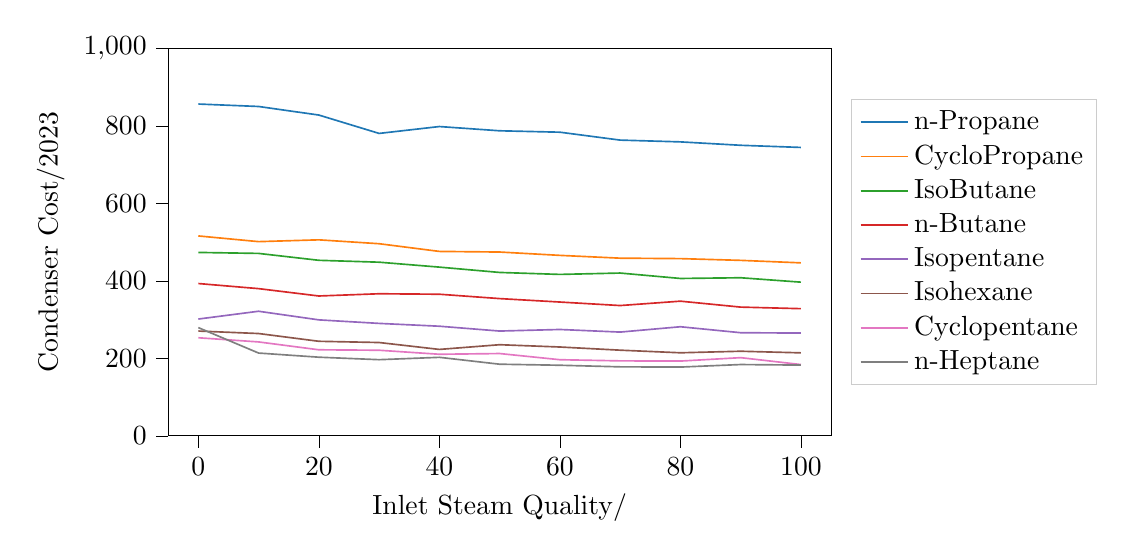
\begin{tikzpicture}

\definecolor{crimson2143940}{RGB}{214,39,40}
\definecolor{darkgray176}{RGB}{176,176,176}
\definecolor{darkorange25512714}{RGB}{255,127,14}
\definecolor{forestgreen4416044}{RGB}{44,160,44}
\definecolor{gray127}{RGB}{127,127,127}
\definecolor{lightgray204}{RGB}{204,204,204}
\definecolor{mediumpurple148103189}{RGB}{148,103,189}
\definecolor{orchid227119194}{RGB}{227,119,194}
\definecolor{sienna1408675}{RGB}{140,86,75}
\definecolor{steelblue31119180}{RGB}{31,119,180}

\begin{axis}[
legend cell align={left},
legend style={fill opacity=0.8, draw opacity=1, text opacity=1, draw=lightgray204, at={(1.03, 0.5)}, anchor=west},
tick align=outside,
tick pos=left,
x grid style={darkgray176},
xlabel={Inlet Steam Quality/\unit{\percent}},
xmin=-5, xmax=105,
xtick style={color=black},
y grid style={darkgray176},
ylabel={Condenser Cost/\unit{\mega\USD\of{2023}}},
ymin=0, ymax=1000,
ytick style={color=black},
width=10cm, height=6.5cm
]
\addplot [semithick, steelblue31119180]
table {%
0 856.609000900582
10 850.281668141461
20 828.151059076382
30 780.737197757208
40 798.493911536669
50 787.529527046714
60 783.882247343145
70 763.468205962579
80 758.887194908456
90 750.089246286169
100 744.530168914593
};
\addlegendentry{n-Propane}
\addplot [semithick, darkorange25512714]
table {%
0 516.020558463637
10 501.30553103517
20 505.951010775091
30 495.930613592412
40 476.058719056902
50 474.465231083977
60 465.846760809336
70 458.597779590553
80 457.455359087093
90 452.955727230435
100 446.518652150664
};
\addlegendentry{CycloPropane}
\addplot [semithick, forestgreen4416044]
table {%
0 473.417755288306
10 470.893654149313
20 453.096463936788
30 448.222594455954
40 435.48606761682
50 421.74408930848
60 416.670607472408
70 420.185272351232
80 406.199944998692
90 408.057194194791
100 396.646477482316
};
\addlegendentry{IsoButane}
\addplot [semithick, crimson2143940]
table {%
0 393.113621184754
10 379.949114674235
20 360.960244683953
30 366.734822249057
40 365.490006366735
50 354.234240925274
60 345.336844113957
70 336.288787694947
80 347.587040781091
90 332.253366975394
100 328.231293348672
};
\addlegendentry{n-Butane}
\addplot [semithick, mediumpurple148103189]
table {%
0 301.427979295675
10 321.553366969466
20 299.276005915914
30 290.18299799146
40 282.907689436532
50 270.425242588046
60 274.477753849377
70 267.771508935847
80 281.535854241728
90 266.121038005447
100 265.256632573786
};
\addlegendentry{Isopentane}
\addplot [semithick, sienna1408675]
table {%
0 270.460227534844
10 264.013186451221
20 243.986067069608
30 240.815973794602
40 223.005487370836
50 235.15299464401
60 229.226864312327
70 221.041169754597
80 214.31395140297
90 218.306473228498
100 214.154437933311
};
\addlegendentry{Isohexane}
\addplot [semithick, orchid227119194]
table {%
0 253.108729399176
10 242.33020515504
20 222.047955860749
30 220.861023593587
40 210.473799515506
50 212.362646025425
60 196.411403710576
70 193.425554516576
80 192.910023851364
90 201.73889288785
100 183.90198272787
};
\addlegendentry{Cyclopentane}
\addplot [semithick, gray127]
table {%
0 279.305900217209
10 213.611355054458
20 202.920760767026
30 196.495202123842
40 202.586078949849
50 184.807072179587
60 182.123581299592
70 178.019934884727
80 177.424316997207
90 183.9607764994
100 182.550130406954
};
\addlegendentry{n-Heptane}
\end{axis}

\end{tikzpicture}

        \caption{The condenser cost fluid normalised by the plant power by working for a geofluid inlet temperature of \qty{548}{\K} as a function of inlet vapour quality.}
        \label{fig:prosim_purewater_spec_cond_cost}
    \end{figure}

\subsection{Direct Comparison}
    \label{sec:thermo_opt_direc_comp}
    To draw a direct comparison between the single flash \ac{DSC} and the binary \ac{ORC} geothermal power plants, a suitable metric must first be chosen to select the optimum binary \ac{ORC} configuration amongst the configurations considered (in this case the different working fluids investigated). 
    
    For instance, if net electrical power is considered the most important, then the for each geofluid inlet condition studied, the binary \ac{ORC} configuration(s) yielding the maximum net electrical power should be selected, Figure~\ref{fig:prosim_purewater_Wnet_DSC_vs_ORC}. For further comparison of plant metrics, such as the specific plant cost, the values corresponding to the selected binary \ac{ORC} configuration(s) should be considered. 

    \begin{figure}[H]
        \centering
        % This file was created with tikzplotlib v0.10.1.
\begin{tikzpicture}

\definecolor{chocolate2369815}{RGB}{236,98,15}
\definecolor{darkgray165}{RGB}{165,165,165}
\definecolor{darkgray176}{RGB}{176,176,176}
\definecolor{darkslategray45}{RGB}{45,45,45}
\definecolor{dimgray108}{RGB}{108,108,108}
\definecolor{firebrick175572}{RGB}{175,57,2}
\definecolor{gainsboro216}{RGB}{216,216,216}
\definecolor{lightgray204}{RGB}{204,204,204}
\definecolor{lightsteelblue157201224}{RGB}{157,201,224}
\definecolor{midnightblue848107}{RGB}{8,48,107}
\definecolor{navajowhite253207161}{RGB}{253,207,161}
\definecolor{powderblue197218238}{RGB}{197,218,238}
\definecolor{saddlebrown127394}{RGB}{127,39,4}
\definecolor{sandybrown25315378}{RGB}{253,153,78}
\definecolor{sandybrown253173106}{RGB}{253,173,106}
\definecolor{silver188}{RGB}{188,188,188}
\definecolor{skyblue127184218}{RGB}{127,184,218}
\definecolor{steelblue59139194}{RGB}{59,139,194}
\definecolor{teal1287160}{RGB}{12,87,160}

\begin{groupplot}[group style={group size=1 by 2}]
\nextgroupplot[
legend cell align={left},
legend style={fill opacity=0.8, draw opacity=1, text opacity=1, draw=lightgray204},
tick align=outside,
tick pos=left,
x grid style={darkgray176},
xlabel={Inlet Steam Quality/\unit{\percent}},
xmin=-5, xmax=105,
xtick style={color=black},
y grid style={darkgray176},
ylabel={Net electric power/\unit{\mega\watt}},
ymin=0, ymax=30,
ytick style={color=black}
]
\addplot [semithick, skyblue127184218]
table {%
0 -1
1 -1
};
\addlegendentry{Binary ORC}
\addplot [semithick, chocolate2369815]
table {%
0 -1
1 -1
};
\addlegendentry{Single flash DSC}
\addplot [semithick, gainsboro216]
table {%
0 1
1 1
};
\addlegendentry{\(T_{geo}^{in}=\)\qty{423}{\K}}
\addplot [semithick, silver188]
table {%
0 1
1 1
};
\addlegendentry{\(T_{geo}^{in}=\)\qty{448}{\K}}
\addplot [semithick, darkgray165]
table {%
0 1
1 1
};
\addlegendentry{\(T_{geo}^{in}=\)\qty{473}{\K}}
\addplot [semithick, dimgray108]
table {%
0 1
1 1
};
\addlegendentry{\(T_{geo}^{in}=\)\qty{498}{\K}}
\addplot [semithick, darkslategray45]
table {%
0 1
1 1
};
\addlegendentry{\(T_{geo}^{in}=\)\qty{523}{\K}}
\addplot [semithick, black]
table {%
0 1
1 1
};
\addlegendentry{\(T_{geo}^{in}=\)\qty{548}{\K}}
\addplot [semithick, powderblue197218238, forget plot]
table {%
0 0.960849687129581
10 2.14458569253811
20 3.23035885785677
30 4.27566680248484
40 5.00700544345708
50 5.86983853781537
60 7.0594488651544
70 7.93193718867346
80 8.93664837449323
100 10.3793750090752
};
\addplot [semithick, lightsteelblue157201224, forget plot]
table {%
0 1.50952974466483
10 2.62305472157002
20 5.13252644589229
30 4.57207068080773
40 5.1310978081115
50 5.87176342204058
60 7.11533208609615
70 7.39108765599484
80 8.22080579508858
100 15.3542513774987
};
\addplot [semithick, skyblue127184218, forget plot]
table {%
0 2.09801582575957
10 3.59825615669869
20 3.89507826651621
30 4.66246522274257
40 5.48383732096798
50 6.32697641805644
60 7.05923199079413
70 8.07467669867112
80 8.93821959686381
100 10.7181908644327
};
\addplot [semithick, steelblue59139194, forget plot]
table {%
0 2.72625581513927
10 4.27047342573569
20 5.72840856540256
30 6.89239857439898
40 8.12016385080602
50 8.88948575778284
60 10.3053070490078
70 11.5409117007058
80 12.6644711957681
100 14.8640801493018
};
\addplot [semithick, teal1287160, forget plot]
table {%
0 3.40981980098837
10 4.70211364120694
20 6.01522355697679
30 7.03110269087159
40 8.1430117390292
50 9.0887040876772
60 10.2269550781848
70 11.1570874630651
80 12.1982183362838
100 14.4174746039932
};
\addplot [semithick, midnightblue848107, forget plot]
table {%
0 4.03006986002843
10 5.40480345953533
20 6.42088686926434
30 7.37991543828771
40 8.37226810980826
50 9.21659321716415
60 10.2901081894353
70 11.1013053206093
80 12.3122709020346
100 14.0852296591021
};
\addplot [semithick, navajowhite253207161, forget plot]
table {%
0 0.557114149477613
10 1.638809379093
20 3.21412473778287
30 4.88993046912543
40 6.40119018667188
50 8.01183196896339
60 9.44767830676006
70 10.8199603723257
80 12.2488536362307
100 15.2483801805043
};
\addplot [semithick, sandybrown253173106, forget plot]
table {%
0 1.08066458863151
10 2.2510134932247
20 3.92997004383771
30 5.74272006643475
40 7.49889052798885
50 9.71407527195079
60 11.2066841203576
70 13.5069457281367
80 14.7331560417993
100 18.7500172587311
};
\addplot [semithick, sandybrown25315378, forget plot]
table {%
0 1.64052050679576
10 2.87437434461262
20 4.43651027514178
30 6.54064816254777
40 8.79912360916101
50 10.7969730793877
60 12.751824036599
70 15.3704403856425
80 17.1222600178921
100 20.7412826958224
};
\addplot [semithick, chocolate2369815, forget plot]
table {%
0 2.30555058647817
10 3.65977973139912
20 4.83127169874635
30 7.24894705666434
40 9.50696724488665
50 11.9924728626009
60 13.6748087725596
70 16.757977411243
80 18.9233907014631
100 23.2626803222292
};
\addplot [semithick, firebrick175572, forget plot]
table {%
0 3.14394468871166
10 4.57715473188939
20 5.88207130807426
30 7.59483919695904
40 10.0956998814759
50 13.0154460785487
60 15.5655359107965
70 17.8582574715776
80 20.0412390531391
100 25.2823359007929
};
\addplot [semithick, saddlebrown127394, forget plot]
table {%
0 4.04694608432612
10 5.56385477936918
20 6.78431620199085
30 8.51801675553119
40 10.9574501504885
50 13.4872385647876
60 16.0443522656724
70 18.7578315602252
80 21.4234178239481
100 26.2259847001766
};
\addplot [semithick, red, mark=*, mark size=3, mark options={solid}, only marks]
table {%
20.2574810001872 3.25727355136542
25.0672234506447 4.84853098630374
15.7209666111048 3.76806709466906
27.155997056422 6.56135947321086
21.9106672040425 6.20932425141718
0 4.04694608432612
};
\addlegendentry{Break-even}

\nextgroupplot[
legend cell align={left},
legend style={fill opacity=0.8, draw opacity=1, text opacity=1, draw=lightgray204},
tick align=outside,
tick pos=left,
x grid style={darkgray176},
xlabel={Inlet Steam Quality/\unit{\percent}},
xmin=-5, xmax=105,
xtick style={color=black},
y grid style={darkgray176},
ylabel={Specific Cost/\unit{\USD\of{2023}\kilo\watt}},
ymin=0, ymax=6000,
ytick style={color=black}
]
\addplot [semithick, powderblue197218238, forget plot]
table {%
0 5019.56547982306
10 2522.57106687602
20 2240.69951062353
30 2053.98683462622
40 1941.96587910678
50 1842.47234948347
60 1780.06832167425
70 1726.41617758276
80 1686.31698562254
100 1602.83504349693
};
\addplot [semithick, lightsteelblue157201224, forget plot]
table {%
0 2744.8946588861
10 2272.38543986691
20 3348.05408810455
30 1882.88408329855
40 1771.02522520651
50 1688.72521989823
60 1631.21205136017
70 1574.09109359846
80 1533.21516140621
100 2205.44172551837
};
\addplot [semithick, skyblue127184218, forget plot]
table {%
0 2405.49149207129
10 3097.84203214475
20 1910.86221173232
30 1786.31917938869
40 1692.84297911923
50 1620.69761919165
60 1608.72937527545
70 1559.30680599622
80 1497.69192144539
100 1417.43111503078
};
\addplot [semithick, steelblue59139194, forget plot]
table {%
0 2198.3771443697
10 2622.27468624185
20 2308.61160681393
30 2113.50877997879
40 1983.50285339464
50 1884.01973590842
60 1785.66175509507
70 1723.64384618247
80 1668.84963609376
100 1569.36440336915
};
\addplot [semithick, teal1287160, forget plot]
table {%
0 2765.12486847892
10 2301.36862785584
20 2055.65553040038
30 1889.16536367077
40 1775.25384422885
50 1688.64847789024
60 1626.58498625757
70 1569.94847324597
80 1501.58429232089
100 1419.16357696616
};
\addplot [semithick, midnightblue848107, forget plot]
table {%
0 2364.49395107708
10 2082.70271598588
20 1902.65310939968
30 1778.30302161461
40 1681.76596511172
50 1605.11369334188
60 1540.95964264706
70 1487.43202350552
80 1443.68293367015
100 1365.31239325101
};
\addplot [semithick, navajowhite253207161, forget plot]
table {%
0 4888.7143335263
10 3404.0250225565
20 2765.54563623294
30 2409.1559187536
40 2183.27858115757
50 2009.69985620321
60 1878.59416928319
70 1781.0224664262
80 1687.7740515826
100 1554.39592832416
};
\addplot [semithick, sandybrown253173106, forget plot]
table {%
0 4151.52655916405
10 3093.66458210808
20 2505.74674359629
30 2179.5159627031
40 1957.18513763749
50 1799.12235928086
60 1671.81829312684
70 1573.71545917379
80 1494.37146800752
100 1352.99672129195
};
\addplot [semithick, sandybrown25315378, forget plot]
table {%
0 3655.98032140456
10 2848.07438984096
20 2334.75521170762
30 2013.49500986261
40 1811.64639061245
50 1658.35478306289
60 1536.22860528175
70 1435.11969747933
80 1358.52998816526
100 1238.4966377997
};
\addplot [semithick, chocolate2369815, forget plot]
table {%
0 3287.81162533514
10 2646.12175390539
20 2229.84454889565
30 1914.53283550025
40 1708.56313786346
50 1561.84904973759
60 1460.04569452233
70 1351.78587022443
80 1276.63372935777
100 1158.48133985561
};
\addplot [semithick, firebrick175572, forget plot]
table {%
0 2990.67224582709
10 2482.06128606799
20 2131.63812586402
30 1851.79844429968
40 1651.15991464286
50 1500.51750608008
60 1386.25897980577
70 1297.77276358557
80 1226.84937810228
100 1105.73508294575
};
\addplot [semithick, saddlebrown127394, forget plot]
table {%
0 2759.98967849107
10 2339.78553853144
20 2056.06477249343
30 1810.13960903689
40 1612.61074215184
50 1466.83729484511
60 1357.69912260723
70 1266.77667555141
80 1194.20844445113
100 1078.92746231424
};
\addplot [semithick, red, mark=*, mark size=3, mark options={solid}, only marks]
table {%
80.5840390695152 1683.87914983252
14.9367985901707 2803.42138647796
8.33516703959791 2982.5772322181
12.3239556472682 2549.38077776425
26.7033895623133 1944.05068581207
33.1523929813526 1747.8707476786
};
\addlegendentry{Break-even}
\end{groupplot}

\end{tikzpicture}

        \caption[The net electrical power and the corresponding specific cost of the single flash \ac{DSC} and the binary \ac{ORC} geothermal power plants.]{The net electrical power (left) and the corresponding specific cost (right) of the single flash \ac{DSC} and the binary \ac{ORC} geothermal power plants. For the binary \ac{ORC},  the net electrical power is the maximum across all working fluids.}
        \label{fig:prosim_purewater_Wnet_DSC_vs_ORC}
    \end{figure}

    From a second law efficiency perspective, the break-even in brute-force efficiencies closely matches the break-even in net electrical power at geofluid inlet vapour qualities between around \qty{55}{\percent} and \qty{85}{\percent}. By contrast, for the functional efficiency the break-even is less dependent on the geofluid inlet vapour quality and occurs at around \qty{45}{\percent}, see Figure~\ref{fig:prosim_purewater_EFF_II_DSC_vs_ORC}. Combined, the two technologies generate electricity at second law efficiencies in excess of \qty{50}{\percent} for temperatures above \qty{200}{\K} irrespective of the geofluid inlet vapour quality.   

    \begin{figure}[H]
        \centering
        % This file was created with tikzplotlib v0.10.1.
\begin{tikzpicture}

\definecolor{chocolate2369815}{RGB}{236,98,15}
\definecolor{darkgray165}{RGB}{165,165,165}
\definecolor{darkgray176}{RGB}{176,176,176}
\definecolor{darkslategray45}{RGB}{45,45,45}
\definecolor{dimgray108}{RGB}{108,108,108}
\definecolor{firebrick175572}{RGB}{175,57,2}
\definecolor{gainsboro216}{RGB}{216,216,216}
\definecolor{lightgray204}{RGB}{204,204,204}
\definecolor{lightsteelblue157201224}{RGB}{157,201,224}
\definecolor{midnightblue848107}{RGB}{8,48,107}
\definecolor{navajowhite253207161}{RGB}{253,207,161}
\definecolor{powderblue197218238}{RGB}{197,218,238}
\definecolor{saddlebrown127394}{RGB}{127,39,4}
\definecolor{sandybrown25315378}{RGB}{253,153,78}
\definecolor{sandybrown253173106}{RGB}{253,173,106}
\definecolor{silver188}{RGB}{188,188,188}
\definecolor{skyblue127184218}{RGB}{127,184,218}
\definecolor{steelblue59139194}{RGB}{59,139,194}
\definecolor{teal1287160}{RGB}{12,87,160}

\begin{groupplot}[
    group style={
        group size=2 by 1, 
        vertical sep=2.5cm, 
        horizontal sep=2.5cm},
    height=6cm, 
    width=7cm, 
]
\nextgroupplot[
legend cell align={left},
legend style={
  fill opacity=0.8,
  draw opacity=1,
  text opacity=1,
  at={(1.15, -0.35)},
  anchor=north,
  draw=lightgray204
},
legend columns=4,
tick align=outside,
tick pos=left,
x grid style={darkgray176},
xlabel={Inlet Steam Quality/\unit{\percent}},
xmin=0, xmax=100,
xtick style={color=black},
y grid style={darkgray176},
ylabel={\(\eta_{bf}^{II}\)/\unit{\percent}},
ymin=0, ymax=100,
ytick style={color=black},
ytick distance=10
]
\addplot [semithick, skyblue127184218]
table {%
0 -1
1 -1
};
\addlegendentry{Binary ORC}
\addplot [semithick, gainsboro216]
table {%
0 1
1 1
};
\addlegendentry{\(T_{geo}^{in}=\)\qty{423}{\K}}
\addplot [semithick, silver188]
table {%
0 1
1 1
};
\addlegendentry{\(T_{geo}^{in}=\)\qty{448}{\K}}
\addplot [semithick, darkgray165]
table {%
0 1
1 1
};
\addlegendentry{\(T_{geo}^{in}=\)\qty{473}{\K}}
\addplot [semithick, chocolate2369815]
table {%
0 -1
1 -1
};
\addlegendentry{Single flash DSC}
\addplot [semithick, dimgray108]
table {%
0 1
1 1
};
\addlegendentry{\(T_{geo}^{in}=\)\qty{498}{\K}}
\addplot [semithick, darkslategray45]
table {%
0 1
1 1
};
\addlegendentry{\(T_{geo}^{in}=\)\qty{523}{\K}}
\addplot [semithick, black]
table {%
0 1
1 1
};
\addlegendentry{\(T_{geo}^{in}=\)\qty{548}{\K}}
\addplot [semithick, powderblue197218238, forget plot]
table {%
0 31.1609685819596
10 49.3638012443299
20 53.0349433067496
30 50.8949627776234
40 49.7404944363951
50 48.5688623284494
60 47.960526744935
70 47.5140406604914
80 46.6007626183509
90 46.6744409019044
100 46.5599082517036
};
\addplot [semithick, lightsteelblue157201224, forget plot]
table {%
0 41.5292956148498
10 50.739186873
20 54.8487893186427
30 59.9056231777704
40 58.3157382468863
50 57.1165608026614
60 56.1430467851468
70 55.4453817454217
80 54.8651160890618
90 54.4593352746145
100 54.0939924676854
};
\addplot [semithick, skyblue127184218, forget plot]
table {%
0 48.2463313832379
10 55.2869153810212
20 58.6050232646661
30 60.7543326151704
40 59.1354313754362
50 57.6571256546261
60 56.938304807727
70 56.0026141386724
80 55.7118019941583
90 55.1728012280721
100 54.6151022923497
};
\addplot [semithick, steelblue59139194, forget plot]
table {%
0 49.5100848590999
10 56.2326770068909
20 61.6157455678554
30 61.2509038144814
40 59.363545551934
50 57.75942384777
60 56.1329734541446
70 55.699270496093
80 55.5903879535986
90 55.4157634383169
100 54.6511769118745
};
\addplot [semithick, teal1287160, forget plot]
table {%
0 52.8898945247783
10 60.5263797138339
20 61.5730986598603
30 60.4304359837121
40 58.7511602369679
50 57.3449787827985
60 56.1142795771936
70 55.6038843344709
80 54.6263561888649
90 53.6802221941346
100 53.8422920321341
};
\addplot [semithick, midnightblue848107, forget plot]
table {%
0 54.673333456994
10 60.5169612555457
20 59.3768801522648
30 57.7215881985748
40 56.3083204689002
50 54.6968171002875
60 54.1413532095568
70 53.3321195306357
80 52.5119536069318
90 51.4724502450234
100 51.4037011677787
};
\addplot [semithick, navajowhite253207161, forget plot]
table {%
0 20.2876531125098
10 28.2983716854617
20 35.784326501965
30 41.3973548257075
40 44.9219324850523
50 47.3224947964041
60 49.1048467808433
70 50.4810687978879
80 51.4999414049741
90 52.3351997147298
100 52.9840146553728
};
\addplot [semithick, sandybrown253173106, forget plot]
table {%
0 23.5318833552946
10 29.8856208745372
20 35.9135606908992
30 41.6208260744231
40 45.8745402628604
50 48.8711591147968
60 51.098344746787
70 52.7920117264809
80 54.1979178588982
90 55.3114292335778
100 56.1399232692997
};
\addplot [semithick, sandybrown25315378, forget plot]
table {%
0 25.9836248849728
10 31.2510498256866
20 36.2731546422741
30 41.1066149422701
40 45.7298293184509
50 49.2857962257922
60 51.6897344726654
70 53.9745105937255
80 55.6862037877521
90 57.0008228744584
100 58.2132743542725
};
\addplot [semithick, chocolate2369815, forget plot]
table {%
0 28.1202452549684
10 32.4289392784475
20 36.7022593995827
30 40.8440792430857
40 45.0047536116939
50 48.8754384063451
60 51.9360917276202
70 54.4124524195702
80 56.3882269931657
90 58.0456097805059
100 59.36011595882
};
\addplot [semithick, firebrick175572, forget plot]
table {%
0 29.8081281102171
10 33.5062767439937
20 37.1514742432
30 40.7488452953087
40 44.3273300529919
50 47.9683484085701
60 51.4100678305885
70 54.2274980428021
80 56.5078474612088
90 58.4512010877023
100 60.1620915361008
};
\addplot [semithick, saddlebrown127394, forget plot]
table {%
0 31.3085300190252
10 34.4787697730121
20 37.5735207933994
30 40.6606262739984
40 43.8087712003011
50 47.0110241435891
60 50.3332215153913
70 53.4679441118929
80 56.1650861195349
90 58.4191284872196
100 60.3503231402517
};
\addplot [semithick, red, mark=*, mark size=3, mark options={solid}, only marks]
table {%
55.2134270857992 48.2517110076145
84.3915070118743 54.6869171598689
80.1380984691528 55.7043584760914
76.1728044702929 55.6320594315883
74.2247944087056 55.19089879008
69.6556133694898 53.3599884566336
};
\addlegendentry{Break-even}

\nextgroupplot[
legend cell align={left},
legend style={
  fill opacity=0.8,
  draw opacity=1,
  text opacity=1,
  at={(0.03,0.03)},
  anchor=south west,
  draw=lightgray204
},
tick align=outside,
tick pos=left,
x grid style={darkgray176},
xlabel={Inlet Steam Quality/\unit{\percent}},
xmin=0, xmax=100,
xtick style={color=black},
y grid style={darkgray176},
ylabel={\(\eta_{func}^{II}\)/\unit{\percent}},
ymin=0, ymax=100,
ytick style={color=black},
ytick distance=10
]
\addplot [semithick, powderblue197218238, forget plot]
table {%
0 45.4975041918806
10 54.4891791470967
20 56.7589384318806
30 54.4680935169156
40 52.9543874199277
50 51.7144492408028
60 51.028589701504
70 50.5179378394815
80 49.5499474479603
90 49.6009308324017
100 49.6334732811971
};
\addplot [semithick, lightsteelblue157201224, forget plot]
table {%
0 52.8178129668459
10 55.6522976296432
20 60.3216459882072
30 63.1367290811166
40 61.3096626226862
50 60.0019990264797
60 58.7966106161852
70 58.0353987629765
80 57.3457648408464
90 56.968336643768
100 56.5738204289271
};
\addplot [semithick, skyblue127184218, forget plot]
table {%
0 53.5288596320671
10 59.8746377403843
20 62.5944295396745
30 63.7543468695528
40 62.0787109341717
50 60.3377922765878
60 59.5308140290528
70 58.6769000586243
80 58.379489104071
90 57.5584766815278
100 57.1376992127984
};
\addplot [semithick, steelblue59139194, forget plot]
table {%
0 55.9510919874033
10 60.807684786037
20 64.7648795814376
30 64.4839648801353
40 61.8169809385292
50 60.5022013855969
60 58.2763387991087
70 57.9269604402395
80 58.6024446863567
90 58.0422789954656
100 57.6838182077878
};
\addplot [semithick, teal1287160, forget plot]
table {%
0 57.5907900996761
10 65.9162708667047
20 65.5066981021631
30 63.7966914331639
40 61.6872803147199
50 59.9552397902744
60 59.0590058153545
70 58.5193328900802
80 57.3441880107545
90 55.6867531779032
100 56.5538941888313
};
\addplot [semithick, midnightblue848107, forget plot]
table {%
0 61.2382346595959
10 64.1322939882725
20 62.7426930974776
30 60.6520188917468
40 59.2108345679003
50 57.1386858922306
60 57.1147088700528
70 56.2122487591182
80 55.2504888294616
90 53.4257846490431
100 53.939152102532
};
\addplot [semithick, navajowhite253207161, forget plot]
table {%
0 39.0928308921832
10 49.0725091397082
20 57.6731737567844
30 58.8239796219953
40 59.2392966099709
50 59.6550705010777
60 60.1280116057264
70 60.6378008052204
80 61.1253867434522
90 61.6397651216655
100 62.2022070355577
};
\addplot [semithick, sandybrown253173106, forget plot]
table {%
0 41.7013020042509
10 48.4075876802402
20 55.2276569341543
30 60.0455757337378
40 60.6443516328184
50 61.2152347834474
60 61.7802041742735
70 62.3759567349422
80 63.0773149167004
90 63.7845689815702
100 64.4616872020477
};
\addplot [semithick, sandybrown25315378, forget plot]
table {%
0 42.835793148178
10 47.8660835727176
20 53.821132660941
30 59.3930199057579
40 61.1727678172062
50 61.8447403007973
60 62.4033586946449
70 63.232545256549
80 64.0525003917748
90 64.8757672303416
100 65.8687770059879
};
\addplot [semithick, chocolate2369815, forget plot]
table {%
0 44.7342442746775
10 47.8407273824714
20 52.8567998511674
30 57.0447575550628
40 59.9938473207944
50 61.7482829835147
60 62.5896521998131
70 63.4941524486697
80 64.3911496479703
90 65.4321153843
100 66.5600435908383
};
\addplot [semithick, firebrick175572, forget plot]
table {%
0 45.3493444988466
10 48.6881163006269
20 51.5171476129728
30 54.6888933404898
40 57.7992772033355
50 60.8390828379274
60 62.2751942484205
70 63.2851590389729
80 64.3392581486818
90 65.5486581107401
100 66.9521414401464
};
\addplot [semithick, saddlebrown127394, forget plot]
table {%
0 46.0018658356573
10 48.6995677201996
20 51.4273229226825
30 53.6180498431893
40 56.364024890237
50 58.8608720519897
60 61.5465751775503
70 62.635987832475
80 63.9232994638279
90 65.3288963675301
100 66.9268550414058
};
\addplot [semithick, red, mark=*, mark size=3, mark options={solid}, only marks]
table {%
18.5559169235394 56.431166334801
43.5416259456335 60.8465370906376
43.7545958933081 61.4250663299369
45.9400644452596 61.0359934109565
48.1477964330868 60.276048954016
46.2307119090511 57.9197384248183
};
\end{groupplot}

\end{tikzpicture}

        \caption[The brute-force and functional second law efficiency of the single flash \ac{DSC} and the binary \ac{ORC} geothermal power plants.]{The brute-force (left) and functional (right) second law efficiency of the single flash \ac{DSC} and the binary \ac{ORC} geothermal power plants. For the binary \ac{ORC},  the maximum efficiency across all working fluids is shown.}
        \label{fig:prosim_purewater_EFF_II_DSC_vs_ORC}
    \end{figure}

    Plotting the geofluid inlet conditions for which the single flash \ac{DSC} and binary \ac{ORC} reach parity, then allows feasibility regions to be identified, Figure~\ref{fig:prosim_purewater_Breakeven_NetPow}. Three regions can be identified:

    \begin{description}
       \item[Region 1] Left of the yellow line (representing parity in specific plant cost), where the binary \ac{ORC} produces more net electrical power and at a lower specific plant cost compared to the single flash \ac{DSC}. 
       \item[Region 2] Between the blue line (representing parity of net electrical power) and yellow line, where the binary \ac{ORC} produces more net electrical power than the single flash \ac{DSC}, albeit at a higher specific cost.
       \item[Region 3] Right of the blue line, where the single flash \ac{DSC} produces more net electrical power and at a lower specific plant cost than the binary \ac{ORC}.
    \end{description}

    \begin{figure}[H]
        \centering
        % This file was created with tikzplotlib v0.10.1.
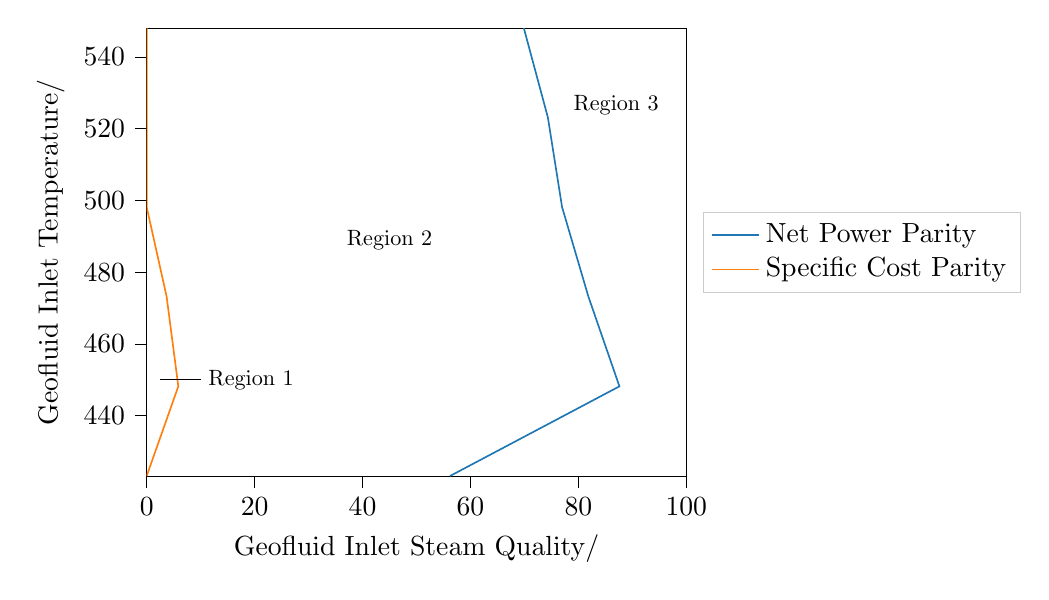
\begin{tikzpicture}

\definecolor{darkgray176}{RGB}{176,176,176}
\definecolor{darkorange25512714}{RGB}{255,127,14}
\definecolor{lightgray204}{RGB}{204,204,204}
\definecolor{steelblue31119180}{RGB}{31,119,180}

\begin{axis}[
legend cell align={left},
legend style={
  fill opacity=0.8,
  draw opacity=1,
  text opacity=1,
  at={(1.03,0.5)},
  anchor=west,
  draw=lightgray204
},
tick align=outside,
tick pos=left,
x grid style={darkgray176},
xlabel={Geofluid Inlet Steam Quality/\unit{\percent}},
xmin=0, xmax=100,
xtick style={color=black},
y grid style={darkgray176},
ylabel={Geofluid Inlet Temperature/\unit{\K}},
ymin=423, ymax=548,
ytick style={color=black}
]
\addplot [semithick, steelblue31119180]
table {%
56.211897840536 423.15
87.6035000467854 448.15
81.8582827723205 473.15
76.9746128225413 498.15
74.343495146738 523.15
69.870082455215 548.15
};
\addlegendentry{Net Power Parity}
\addplot [semithick, darkorange25512714]
table {%
0 423.15
5.86239070301085 448.15
3.70072396216428 473.15
0 498.15
0 523.15
0 548.15
};
\addlegendentry{Specific Cost Parity}
\draw (axis cs:87,525) node[
  scale=0.8,
  anchor=base,
  text=black,
  rotate=0.0
]{Region 3};
\draw (axis cs:45,487.5) node[
  scale=0.8,
  anchor=base,
  text=black,
  rotate=0.0
]{Region 2};
\draw[-,draw=black] (axis cs:10,450) -- (axis cs:2.5,450);
\draw (axis cs:10,450) node[
  scale=0.8,
  anchor=west,
  text=black,
  rotate=0.0
]{Region 1};
\end{axis}

\end{tikzpicture}

        \caption[The geofluid inlet conditions for which the binary \ac{ORC} and single flash \ac{DSC} geothermal power plants deliver equal net electrical power and have equal specific plant cost.]{The geofluid inlet conditions for which the binary \ac{ORC} and single flash \ac{DSC} geothermal power plants deliver equal net electrical power and have equal specific plant cost. For the binary \ac{ORC},  the net electrical power is the maximum across all working fluids.}
        \label{fig:prosim_purewater_Breakeven_NetPow}
    \end{figure}

    \begin{notes}{Note}
        The \emph{kink} in \emph{Net Power Parity} line in Figure~\ref{fig:prosim_purewater_Breakeven_NetPow} can be attributed a change in working fluid. While the upper part of the line follows the net power parity inlet conditions of Cyclopentane, at the lowest temperature considered (\qty{423}{\K}) Cyclopentane is not a viable working fluid, as such the next best viable working fluid, Isohexane, is selected, see Figure~\ref{fig:prosim_purewater_Breakeven_NetPow_by_WF}.

        \begin{figure}[H]
            \centering
            % This file was created with tikzplotlib v0.10.1.
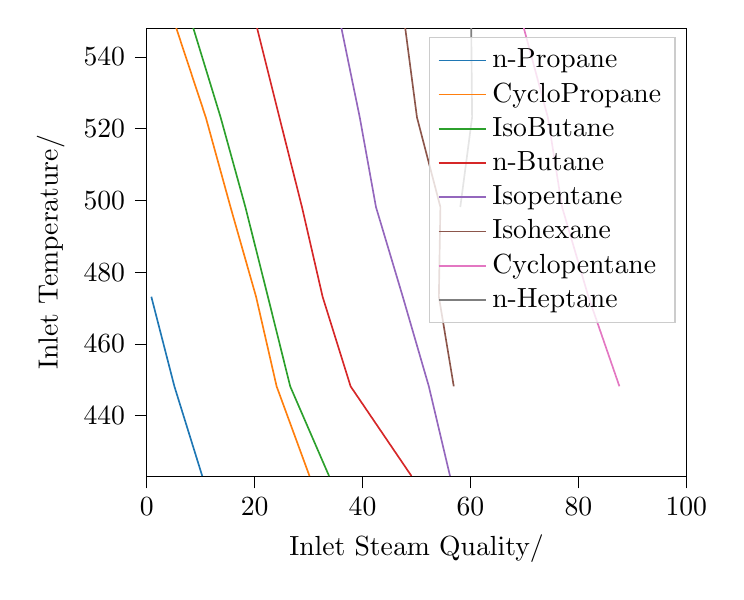
\begin{tikzpicture}

\definecolor{crimson2143940}{RGB}{214,39,40}
\definecolor{darkgray176}{RGB}{176,176,176}
\definecolor{darkorange25512714}{RGB}{255,127,14}
\definecolor{forestgreen4416044}{RGB}{44,160,44}
\definecolor{gray127}{RGB}{127,127,127}
\definecolor{lightgray204}{RGB}{204,204,204}
\definecolor{mediumpurple148103189}{RGB}{148,103,189}
\definecolor{orchid227119194}{RGB}{227,119,194}
\definecolor{sienna1408675}{RGB}{140,86,75}
\definecolor{steelblue31119180}{RGB}{31,119,180}

\begin{axis}[
legend cell align={left},
legend style={fill opacity=0.8, draw opacity=1, text opacity=1, draw=lightgray204},
tick align=outside,
tick pos=left,
x grid style={darkgray176},
xlabel={Inlet Steam Quality/\unit{\percent}},
xmin=0, xmax=100,
xtick style={color=black},
y grid style={darkgray176},
ylabel={Inlet Temperature/\unit{\K}},
ymin=423, ymax=548,
ytick style={color=black}
]
\addplot [semithick, steelblue31119180]
table {%
0.860432064814202 473.15
5.1366254880995 448.15
10.2982809248621 423.15
};
\addlegendentry{n-Propane}
\addplot [semithick, darkorange25512714]
table {%
5.45981774483597 548.15
10.9569527334517 523.15
15.5342645550449 498.15
20.2698916289944 473.15
24.0782774108881 448.15
30.1732199888322 423.15
};
\addlegendentry{CycloPropane}
\addplot [semithick, forestgreen4416044]
table {%
8.61667934959712 548.15
13.7038897374226 523.15
18.2895197571598 498.15
22.4640798058543 473.15
26.5962038137456 448.15
33.7983725758173 423.15
};
\addlegendentry{IsoButane}
\addplot [semithick, crimson2143940]
table {%
20.4394782095746 548.15
24.595078256838 523.15
28.7760448540457 498.15
32.5990272774492 473.15
37.7893009240293 448.15
49.0688623012555 423.15
};
\addlegendentry{n-Butane}
\addplot [semithick, mediumpurple148103189]
table {%
36.0711120192674 548.15
39.4863149169637 523.15
42.4891596723533 498.15
47.4578869347348 473.15
52.2869142724592 448.15
56.211897840536 423.15
};
\addlegendentry{Isopentane}
\addplot [semithick, sienna1408675]
table {%
47.9031536469212 548.15
50.0856527082001 523.15
54.4267883039785 498.15
54.1464763172917 473.15
56.9070485383301 448.15
};
\addlegendentry{Isohexane}
\addplot [semithick, orchid227119194]
table {%
69.870082455215 548.15
74.343495146738 523.15
76.9746128225413 498.15
81.8582827723205 473.15
87.6035000467854 448.15
};
\addlegendentry{Cyclopentane}
\addplot [semithick, gray127]
table {%
60.143064588981 548.15
60.3041199838426 523.15
58.1184303215883 498.15
};
\addlegendentry{n-Heptane}
\end{axis}

\end{tikzpicture}

            \caption{The geofluid inlet conditions for which the binary \ac{ORC} and single flash \ac{DSC} geothermal power plants deliver equal net electrical power by working fluid.}
            \label{fig:prosim_purewater_Breakeven_NetPow_by_WF}
        \end{figure}
        
    \end{notes}

    % Safe this for later
    % This can be attributed to the binary \ac{ORC} being capable of utilising the entire heat content of the geofluid, while \ac{DSC} is only able to utilise the vapour portion. For instance, for a geofluid arriving at \qty{473}{\K} and a vapour quality of \qty{20}{\percent}, the vapour carries only about \qty{45}{\percent} of the total enthalpy entering the plant.

    Similarly, if the specific cost is considered the most important metric, then the for each geofluid inlet condition studied, the binary \ac{ORC} configuration(s) yielding the minimum specific plant cost should be selected, Figure~\ref{fig:prosim_purewater_SpecCost_DSC_vs_ORC}. The same three region are observed, however their spread is reduced, and Region 1 extends to higher geofluid inlet vapour qualities for all temperatures (about \qty{20}{\percent}). 

    % However, from a cost perspective, the \ac{DSC} geothermal power plants are favourable for geofluid inlet vapour qualities higher than \qty{10}{\percent}, Figures~\ref{fig:prosim_purewater_SpecCost_DSC_vs_ORC} and \ref{fig:prosim_purewater_Breakeven_DSC_vs_ORC}. While the steam turbine costs are comparable to many of the heavier \ac{ORC} working fluids, for the working fluid with the lowest specific plant cost, it is the difference in condenser costs and the lack of a \ac{PHE} unit that makes the \ac{DSC} economically favourable. 

    \begin{figure}[H]
        \centering
        % This file was created with tikzplotlib v0.10.1.
\begin{tikzpicture}

\definecolor{chocolate2369815}{RGB}{236,98,15}
\definecolor{darkgray165}{RGB}{165,165,165}
\definecolor{darkgray176}{RGB}{176,176,176}
\definecolor{darkslategray45}{RGB}{45,45,45}
\definecolor{dimgray108}{RGB}{108,108,108}
\definecolor{firebrick175572}{RGB}{175,57,2}
\definecolor{gainsboro216}{RGB}{216,216,216}
\definecolor{lightgray204}{RGB}{204,204,204}
\definecolor{lightsteelblue157201224}{RGB}{157,201,224}
\definecolor{midnightblue848107}{RGB}{8,48,107}
\definecolor{navajowhite253207161}{RGB}{253,207,161}
\definecolor{powderblue197218238}{RGB}{197,218,238}
\definecolor{saddlebrown127394}{RGB}{127,39,4}
\definecolor{sandybrown25315378}{RGB}{253,153,78}
\definecolor{sandybrown253173106}{RGB}{253,173,106}
\definecolor{silver188}{RGB}{188,188,188}
\definecolor{skyblue127184218}{RGB}{127,184,218}
\definecolor{steelblue59139194}{RGB}{59,139,194}
\definecolor{teal1287160}{RGB}{12,87,160}

\begin{groupplot}[group style={group size=1 by 2}]
\nextgroupplot[
legend cell align={left},
legend style={fill opacity=0.8, draw opacity=1, text opacity=1, draw=lightgray204},
tick align=outside,
tick pos=left,
x grid style={darkgray176},
xlabel={Inlet Steam Quality/\unit{\percent}},
xmin=-5, xmax=105,
xtick style={color=black},
y grid style={darkgray176},
ylabel={Specific Cost/\unit{\USD\of{2023}\kilo\watt}},
ymin=0, ymax=6000,
ytick style={color=black}
]
\addplot [semithick, skyblue127184218]
table {%
0 1
1 1
};
\addlegendentry{Binary ORC}
\addplot [semithick, chocolate2369815]
table {%
0 1
1 1
};
\addlegendentry{Single flash DSC}
\addplot [semithick, gainsboro216]
table {%
0 1
1 1
};
\addlegendentry{\(T_{geo}^{in}=\)\qty{423}{\K}}
\addplot [semithick, silver188]
table {%
0 1
1 1
};
\addlegendentry{\(T_{geo}^{in}=\)\qty{448}{\K}}
\addplot [semithick, darkgray165]
table {%
0 1
1 1
};
\addlegendentry{\(T_{geo}^{in}=\)\qty{473}{\K}}
\addplot [semithick, dimgray108]
table {%
0 1
1 1
};
\addlegendentry{\(T_{geo}^{in}=\)\qty{498}{\K}}
\addplot [semithick, darkslategray45]
table {%
0 1
1 1
};
\addlegendentry{\(T_{geo}^{in}=\)\qty{523}{\K}}
\addplot [semithick, black]
table {%
0 1
1 1
};
\addlegendentry{\(T_{geo}^{in}=\)\qty{548}{\K}}
\addplot [semithick, powderblue197218238, forget plot]
table {%
0 4117.01145790712
10 3783.79307127179
20 3277.26496537247
30 2885.83060038486
40 2656.88510105255
50 2536.98129798443
60 2399.92027092259
70 2319.33618155377
80 2256.56992800507
90 2198.84722936431
100 2155.76951812054
};
\addplot [semithick, lightsteelblue157201224, forget plot]
table {%
0 4029.44230073587
10 3642.65226356929
20 2868.92887945694
30 2489.35808638132
40 2306.02690091309
50 2194.26850678537
60 2106.59876178413
70 2039.41301512096
80 1983.63481498905
90 1932.14886330554
100 1878.31732336987
};
\addplot [semithick, skyblue127184218, forget plot]
table {%
0 3585.04906524689
10 3062.95078885213
20 2601.17267795214
30 2369.45547809689
40 2183.42127474037
50 2088.17516605231
60 1989.79208588077
70 1937.15559430886
80 1880.15962224779
90 1827.92110615512
100 1784.4193788523
};
\addplot [semithick, steelblue59139194, forget plot]
table {%
0 3491.68852578916
10 2806.34893142611
20 2440.9865908632
30 2258.44513282194
40 2150.75196042525
50 2034.4618935711
60 1955.37708447813
70 1929.28337237939
80 1847.95728199719
90 1795.39877551786
100 1745.9490823015
};
\addplot [semithick, teal1287160, forget plot]
table {%
0 2927.37542690606
10 2548.05853688079
20 2345.34176091862
30 2195.68613503973
40 2064.77806427466
50 1987.38617608607
60 1912.96108394623
70 1857.05789687585
80 1813.56632871972
90 1771.72803343882
100 1730.33619163488
};
\addplot [semithick, midnightblue848107, forget plot]
table {%
0 2631.00541665103
10 2395.11796420667
20 2209.91996902185
30 2141.15005612907
40 2068.73044333239
50 1977.637505201
60 1894.86025458744
70 1825.78126517306
80 1779.4294219757
90 1761.74684698698
100 1673.20129902748
};
\addplot [semithick, navajowhite253207161, forget plot]
table {%
0 5397.87889906703
10 3768.29270492488
20 2972.77549062956
30 2595.59903943147
40 2356.89776792824
50 2182.49680235925
60 2046.68855521956
70 1936.77197539381
80 1844.9470110938
90 1768.1882260683
100 1698.50453307752
};
\addplot [semithick, sandybrown253173106, forget plot]
table {%
0 4553.23201853484
10 3404.12568059557
20 2750.02155834648
30 2338.40989961059
40 2112.53568938616
50 1947.98212479846
60 1821.86395592416
70 1719.56546058179
80 1633.92926564459
90 1561.93392933804
100 1500.04333525452
};
\addplot [semithick, sandybrown25315378, forget plot]
table {%
0 3997.591337054
10 3127.91569148296
20 2572.52535475938
30 2188.20053767263
40 1953.30434225776
50 1797.74666476365
60 1672.2143192466
70 1578.73530661691
80 1498.53083730244
90 1430.09446218898
100 1371.73706471868
};
\addplot [semithick, chocolate2369815, forget plot]
table {%
0 3549.64809783391
10 2897.23230903276
20 2429.89306471283
30 2103.22460391644
40 1869.11159709999
50 1699.98113196286
60 1581.30868606629
70 1486.45117067198
80 1410.2843034799
90 1344.69043048712
100 1285.6882429292
};
\addplot [semithick, firebrick175572, forget plot]
table {%
0 3226.82549267642
10 2688.90676066591
20 2325.75230073436
30 2046.54231571548
40 1825.64459127168
50 1644.53344341149
60 1519.78143988873
70 1426.9685532797
80 1350.86351200683
90 1286.85504034817
100 1232.59923079975
};
\addplot [semithick, saddlebrown127394, forget plot]
table {%
0 2958.66976346962
10 2533.37988676905
20 2219.38817607804
30 1986.18834016362
40 1789.29486320968
50 1628.54153899057
60 1484.71067372609
70 1393.578164606
80 1317.58503166833
90 1253.56802416479
100 1199.23934850659
};
\addplot [semithick, red, mark=*, mark size=3, mark options={solid}, only marks]
table {%
9.88043234136831 3787.77728550209
6.87102869593706 3763.67775626845
16.9397882658249 2742.48655730827
18.9121530717588 2480.73242085083
18.7789988175102 2370.09350323465
20.5758201963607 2205.96005854729
};
\addlegendentry{Break-even}

\nextgroupplot[
tick align=outside,
tick pos=left,
x grid style={darkgray176},
xlabel={Inlet Steam Quality/\unit{\percent}},
xmin=-5, xmax=105,
xtick style={color=black},
y grid style={darkgray176},
ylabel={Net electric power/\unit{\mega\watt}},
ymin=0, ymax=30,
ytick style={color=black}
]
\addplot [semithick, powderblue197218238]
table {%
0 1.23605473349593
10 3.5756072888753
20 4.38840529184303
30 5.46189923594778
40 6.48976611771234
50 7.58614921737993
60 8.63847561605714
70 9.70373614856986
80 10.7596993623872
90 11.835366302188
100 12.8708089665906
};
\addplot [semithick, lightsteelblue157201224]
table {%
0 2.18417660227053
10 4.64737177870483
20 5.95606611315968
30 7.20175010897652
40 8.45050815445565
50 9.69176142416153
60 10.8923606719086
70 12.1802896588963
80 13.4370912870973
90 14.691049141923
100 15.962768565911
};
\addplot [semithick, skyblue127184218]
table {%
0 3.75045845803564
10 5.3233703834005
20 6.52143371948183
30 7.72325173820182
40 8.90734085878374
50 10.0900882744848
60 11.2859816404375
70 12.4799494051215
80 13.6582927603204
90 14.8580333710726
100 16.0578783341511
};
\addplot [semithick, steelblue59139194]
table {%
0 4.80339701119718
10 5.96167414778747
20 7.0886078874336
30 8.22014410954725
40 9.34712087668599
50 10.4708956712552
60 11.6094636572235
70 12.7332688105754
80 13.8550959632211
90 14.9815179684654
100 16.1238187732451
};
\addplot [semithick, teal1287160]
table {%
0 5.56624744040748
10 6.61781825102425
20 7.67523188177118
30 8.715590812771
40 9.75364620420889
50 10.8054575156457
60 11.887534375607
70 12.9449823333358
80 13.9996307255139
90 15.0346834881891
100 16.1046299241576
};
\addplot [semithick, midnightblue848107]
table {%
0 6.32348038479448
10 7.27355075494739
20 8.24488357844434
30 9.21668949583969
40 10.1917076371687
50 11.1674060349929
60 19.2969638942651
70 20.8304609730809
80 22.3119648153803
90 15.01376552939
100 25.3608303451308
};
\addplot [semithick, navajowhite253207161]
table {%
0 0.848766335311801
10 2.02965916823412
20 3.63678012234456
30 5.44833428255714
40 7.25930671017054
50 9.0662679860003
60 10.8803147696488
70 12.6991628508844
80 14.4995989214377
90 16.3042529392927
100 18.0943906521875
};
\addplot [semithick, sandybrown253173106]
table {%
0 1.37298923719255
10 2.7159042785621
20 4.43218820144198
30 6.49193207610785
40 8.651963212448
50 10.8113503472737
60 12.9710914641018
70 15.1231233082903
80 17.2939633303419
90 19.4536693432826
100 21.5760042101645
};
\addplot [semithick, sandybrown25315378]
table {%
0 2.00704976317278
10 3.48622124228406
20 5.29070301214816
30 7.40602998595349
40 9.81065940251747
50 12.2687276928164
60 14.6430124095696
70 17.1478727162591
80 19.6069623546236
90 22.0296823002723
100 24.5007022429487
};
\addplot [semithick, chocolate2369815]
table {%
0 2.77203624120037
10 4.33961104553125
20 6.20418692713397
30 8.34349028695991
40 10.7804704280669
50 13.4322474411363
60 16.1066765210045
70 18.7955337328933
80 21.4689540327441
90 24.1492382123889
100 26.7903244331684
};
\addplot [semithick, firebrick175572]
table {%
0 3.65272804686847
10 5.28756622552709
20 7.17354497696852
30 9.30569577039438
40 11.6868609499473
50 14.3397742532943
60 17.1845519572385
70 20.0420402295364
80 22.8808897324396
90 25.7327822006828
100 28.612139819668
};
\addplot [semithick, saddlebrown127394]
table {%
0 4.68019046356514
10 6.33786824208722
20 8.19662468617633
30 10.2665258268757
40 12.5659729496647
50 15.0996305321506
60 17.8961824166246
70 20.8488991260731
80 23.8316642482924
90 26.7962209044811
100 29.7567639294773
};
\addplot [semithick, red, mark=*, mark size=3, mark options={solid}, only marks]
table {%
30.1732199888322 5.4797039449258
37.7893009240293 8.17444532873048
32.5990272774492 8.03099973053415
28.7760448540457 8.08164915135828
24.595078256838 8.15328495208563
20.4394782095746 8.28759233090743
};
\end{groupplot}

\end{tikzpicture}

        \caption[The specific plant cost and the corresponding net electrical power of the single flash \ac{DSC} and the binary \ac{ORC}.]{The specific plant cost (left) and the corresponding net electrical power (right) of the single flash \ac{DSC} and the binary \ac{ORC}. For the binary \ac{ORC}, the specific plant cost is the minimum across all working fluids considered.}
        \label{fig:prosim_purewater_SpecCost_DSC_vs_ORC}
    \end{figure}  

    \begin{figure}[H]
        \centering
        % This file was created with tikzplotlib v0.10.1.
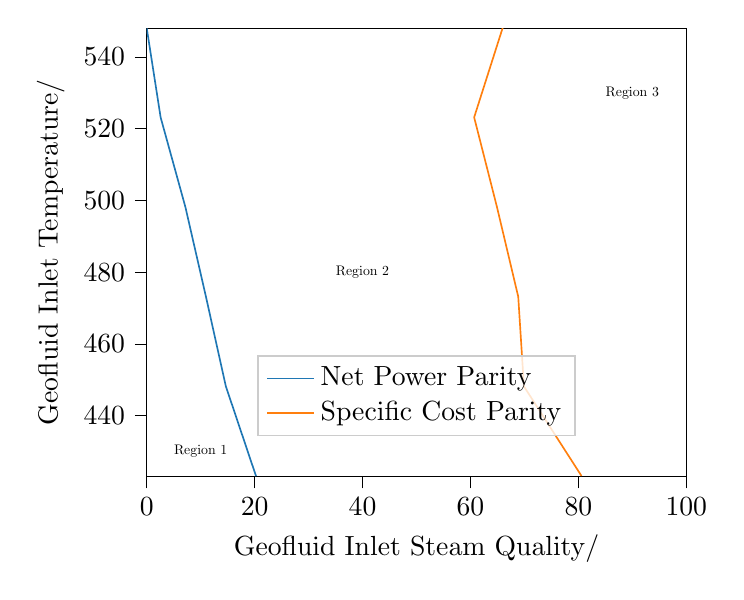
\begin{tikzpicture}

\definecolor{darkgray176}{RGB}{176,176,176}
\definecolor{darkorange25512714}{RGB}{255,127,14}
\definecolor{lightgray204}{RGB}{204,204,204}
\definecolor{steelblue31119180}{RGB}{31,119,180}

\begin{axis}[
legend cell align={left},
legend style={
  fill opacity=0.8,
  draw opacity=1,
  text opacity=1,
  at={(0.5,0.09)},
  anchor=south,
  draw=lightgray204
},
tick align=outside,
tick pos=left,
x grid style={darkgray176},
xlabel={Geofluid Inlet Steam Quality/\unit{\percent}},
xmin=0, xmax=100,
xtick style={color=black},
y grid style={darkgray176},
ylabel={Geofluid Inlet Temperature/\unit{\K}},
ymin=423, ymax=548,
ytick style={color=black}
]
\addplot [semithick, steelblue31119180]
table {%
20.2574810001872 423.15
14.6736248492937 448.15
10.9828903695487 473.15
7.17456971654515 498.15
2.5857550533881 523.15
0 548.15
};
\addlegendentry{Net Power Parity}
\addplot [semithick, darkorange25512714]
table {%
80.5840390695152 423.15
69.9083413304653 448.15
68.8529408109643 473.15
64.9111763437638 498.15
60.6841000655588 523.15
65.9803998207952 548.15
};
\addlegendentry{Specific Cost Parity}
\draw (axis cs:10,430) node[
  scale=0.5,
  text=black,
  rotate=0.0
]{Region 1};
\draw (axis cs:40,480) node[
  scale=0.5,
  text=black,
  rotate=0.0
]{Region 2};
\draw (axis cs:90,530) node[
  scale=0.5,
  text=black,
  rotate=0.0
]{Region 3};
\end{axis}

\end{tikzpicture}

        \caption[The geofluid inlet conditions for which binary \ac{ORC} and single flash \ac{DSC} geothermal power plants deliver equal net electrical power and have equal specific plant costs.]{The geofluid inlet conditions for which binary \ac{ORC} and single flash \ac{DSC} geothermal power plants deliver equal net electrical power and have equal specific plant costs. For the binary \ac{ORC}, the specific plant cost is the minimum across all working fluids considered.}
        \label{fig:prosim_purewater_Breakeven_SpecCost}
    \end{figure}

    % \begin{figure}[H]
    %     \centering
    %     % This file was created with tikzplotlib v0.10.1.
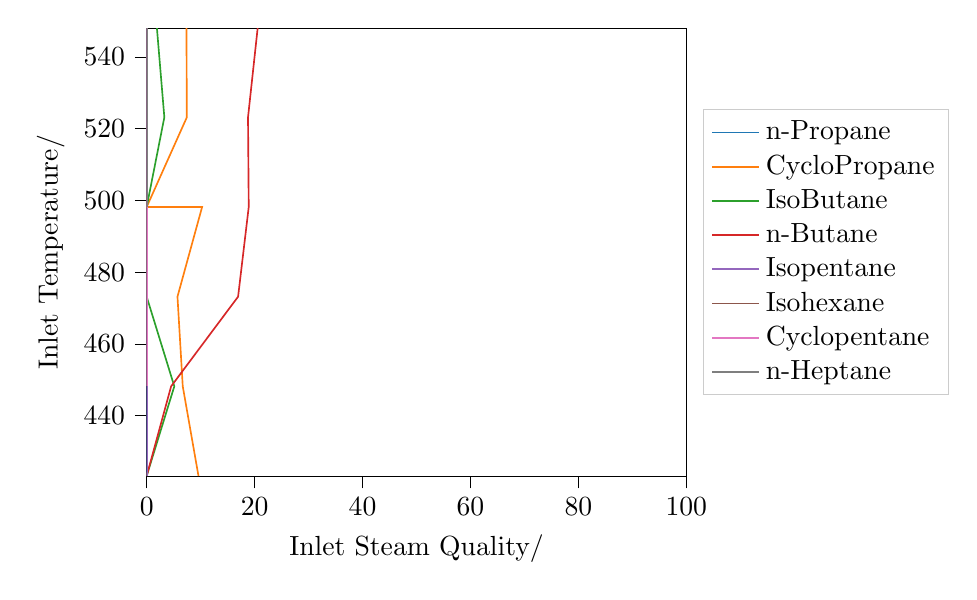
\begin{tikzpicture}

\definecolor{crimson2143940}{RGB}{214,39,40}
\definecolor{darkgray176}{RGB}{176,176,176}
\definecolor{darkorange25512714}{RGB}{255,127,14}
\definecolor{forestgreen4416044}{RGB}{44,160,44}
\definecolor{gray127}{RGB}{127,127,127}
\definecolor{lightgray204}{RGB}{204,204,204}
\definecolor{mediumpurple148103189}{RGB}{148,103,189}
\definecolor{orchid227119194}{RGB}{227,119,194}
\definecolor{sienna1408675}{RGB}{140,86,75}
\definecolor{steelblue31119180}{RGB}{31,119,180}

\begin{axis}[
legend cell align={left},
legend style={fill opacity=0.8, draw opacity=1, text opacity=1, draw=lightgray204, at={(1.03, 0.5)}, anchor=west},
tick align=outside,
tick pos=left,
x grid style={darkgray176},
xlabel={Inlet Steam Quality/\unit{\percent}},
xmin=0, xmax=100,
xtick style={color=black},
y grid style={darkgray176},
ylabel={Inlet Temperature/\unit{\K}},
ymin=423, ymax=548,
ytick style={color=black}
]
\addplot [semithick, steelblue31119180]
table {%
0 548.15
0 523.15
0 498.15
0 473.15
0 448.15
0 423.15
};
\addlegendentry{n-Propane}
\addplot [semithick, darkorange25512714]
table {%
7.37459290074186 548.15
7.44024453282398 523.15
0 498.15
10.2728103470557 498.15
5.70867385369574 473.15
6.68611121421122 448.15
9.60181428355033 423.15
};
\addlegendentry{CycloPropane}
\addplot [semithick, forestgreen4416044]
table {%
1.89072290870401 548.15
3.27471307641813 523.15
0 498.15
0 473.15
5.12368290885298 448.15
0 423.15
};
\addlegendentry{IsoButane}
\addplot [semithick, crimson2143940]
table {%
20.5758201963607 548.15
18.7789988175102 523.15
18.9121530717588 498.15
16.939788265825 473.15
4.53004342488796 448.15
0 423.15
};
\addlegendentry{n-Butane}
\addplot [semithick, mediumpurple148103189]
table {%
0 548.15
0 523.15
0 498.15
0 473.15
0 448.15
0 423.15
};
\addlegendentry{Isopentane}
\addplot [semithick, sienna1408675]
table {%
0 548.15
0 523.15
0 498.15
0 473.15
0 448.15
};
\addlegendentry{Isohexane}
\addplot [semithick, orchid227119194]
table {%
0 548.15
0 523.15
0 498.15
0 473.15
0 448.15
};
\addlegendentry{Cyclopentane}
\addplot [semithick, gray127]
table {%
0 548.15
0 523.15
0 498.15
};
\addlegendentry{n-Heptane}
\end{axis}

\end{tikzpicture}

    %     \caption{To be removed. The geofluid inlet conditions for which the binary \ac{ORC} and single flash \ac{DSC} geothermal power plants have equal specific plant costs by working fluid.}
    % \end{figure}

    % \begin{figure}[H]
    %     \centering
    %     % This file was created with tikzplotlib v0.10.1.
\begin{tikzpicture}

\definecolor{chocolate2369815}{RGB}{236,98,15}
\definecolor{darkgray165}{RGB}{165,165,165}
\definecolor{darkgray176}{RGB}{176,176,176}
\definecolor{darkslategray45}{RGB}{45,45,45}
\definecolor{dimgray108}{RGB}{108,108,108}
\definecolor{firebrick175572}{RGB}{175,57,2}
\definecolor{gainsboro216}{RGB}{216,216,216}
\definecolor{lightgray204}{RGB}{204,204,204}
\definecolor{lightsteelblue157201224}{RGB}{157,201,224}
\definecolor{midnightblue848107}{RGB}{8,48,107}
\definecolor{navajowhite253207161}{RGB}{253,207,161}
\definecolor{powderblue197218238}{RGB}{197,218,238}
\definecolor{saddlebrown127394}{RGB}{127,39,4}
\definecolor{sandybrown25315378}{RGB}{253,153,78}
\definecolor{sandybrown253173106}{RGB}{253,173,106}
\definecolor{silver188}{RGB}{188,188,188}
\definecolor{skyblue127184218}{RGB}{127,184,218}
\definecolor{steelblue59139194}{RGB}{59,139,194}
\definecolor{teal1287160}{RGB}{12,87,160}

\begin{axis}[
legend cell align={left},
legend style={
  fill opacity=0.8,
  draw opacity=1,
  text opacity=1,
  at={(1.03,0.5)},
  anchor=west,
  draw=lightgray204
},
tick align=outside,
tick pos=left,
x grid style={darkgray176},
xlabel={Inlet Steam Quality/\unit{\percent}},
xmin=-5, xmax=105,
xtick style={color=black},
y grid style={darkgray176},
ylabel={LCOE/\unit{\USD\of{2023}\per\MWh}},
ymin=0, ymax=95.2412225563262,
ytick style={color=black},
width=10cm, height=6.5cm
]
\addplot [semithick, skyblue127184218]
table {%
0 -1
1 -1
};
\addlegendentry{Thermodynamic Opt.}
\addplot [semithick, chocolate2369815]
table {%
0 -1
1 -1
};
\addlegendentry{Techno-economic Opt.}
\addplot [semithick, gainsboro216]
table {%
0 -1
1 -1
};
\addlegendentry{\(T_{geo}^{in}=\)\qty{423}{\K}}
\addplot [semithick, silver188]
table {%
0 -1
1 -1
};
\addlegendentry{\(T_{geo}^{in}=\)\qty{448}{\K}}
\addplot [semithick, darkgray165]
table {%
0 -1
1 -1
};
\addlegendentry{\(T_{geo}^{in}=\)\qty{473}{\K}}
\addplot [semithick, dimgray108]
table {%
0 -1
1 -1
};
\addlegendentry{\(T_{geo}^{in}=\)\qty{498}{\K}}
\addplot [semithick, darkslategray45]
table {%
0 -1
1 -1
};
\addlegendentry{\(T_{geo}^{in}=\)\qty{523}{\K}}
\addplot [semithick, black]
table {%
0 -1
1 -1
};
\addlegendentry{\(T_{geo}^{in}=\)\qty{548}{\K}}
\addplot [semithick, powderblue197218238, forget plot]
table {%
0 90.6583071965011
10 84.0310818887662
20 72.2737154668601
30 63.5871080819099
40 58.6101932969457
50 55.9102561808189
60 52.9691672564642
70 51.1875523161685
80 49.7938636043741
90 48.5193174892524
100 47.5659053885652
};
\addplot [semithick, lightsteelblue157201224, forget plot]
table {%
0 88.1867614919631
10 80.6941825232629
20 63.8409124955318
30 55.5288711213873
40 51.4617417519294
50 48.9659253013169
60 47.016221383792
70 45.5025652125277
80 44.2393784046589
90 43.0951938028827
100 41.8934778849503
};
\addplot [semithick, skyblue127184218, forget plot]
table {%
0 79.7980510215401
10 68.3411619621519
20 57.9655853783276
30 52.8082180199367
40 48.7289231137485
50 46.5999882020035
60 44.4209352237552
70 43.230915184305
80 41.9605391494199
90 40.7965357918193
100 39.8231967263325
};
\addplot [semithick, steelblue59139194, forget plot]
table {%
0 77.7861485339713
10 62.4299597888963
20 54.4255267036977
30 50.3737502972331
40 47.9511490567326
50 45.3965599651333
60 43.6309681897607
70 43.0004132817441
80 41.2286863224372
90 40.0611821902413
100 38.9657152764291
};
\addplot [semithick, teal1287160, forget plot]
table {%
0 65.2381228229504
10 56.7853159389337
20 52.267030625297
30 48.9663333242235
40 46.0870144827189
50 44.3583500780843
60 42.6973245480908
70 41.4477162563803
80 40.4714988694263
90 39.5398016985733
100 38.614669847406
};
\addplot [semithick, midnightblue848107, forget plot]
table {%
0 58.6185075695539
10 53.4049668259427
20 49.3284518217783
30 47.7430826686359
40 46.1021097996825
50 44.096865884123
60 42.4842730788587
70 41.0194172557534
80 40.1019574736714
90 39.3165068256748
100 37.69951247739
};
\addplot [semithick, navajowhite253207161, forget plot]
table {%
0 87.2291394678071
10 63.7119413056852
20 55.6852205734553
30 50.3975575665353
40 47.5243306086635
50 45.2781719056648
60 43.1279149657673
70 42.1293341017887
80 40.5539055166915
100 38.5616356370198
};
\addplot [semithick, sandybrown253173106, forget plot]
table {%
0 69.2802682223896
10 53.6882268634588
20 46.8841182624463
30 43.0073311818876
40 40.4851391610946
50 38.2412026186124
60 36.9056286553239
70 35.5338773060914
80 34.2886407780947
100 32.5630807737716
};
\addplot [semithick, sandybrown25315378, forget plot]
table {%
0 58.5664746481522
10 47.7361920291882
20 42.1594634622475
30 39.6261648301639
40 37.260822793148
50 35.3250091018566
60 33.1023180945567
70 32.0964285690076
80 31.7589773453615
100 29.5075998368524
};
\addplot [semithick, chocolate2369815, forget plot]
table {%
0 50.3709875213588
10 45.0324857443901
20 40.4214502308899
30 38.9131815950235
40 34.8556756583711
50 33.8412434551296
60 31.9243716606042
70 30.6920703508383
80 29.7199113837673
100 28.7705175936364
};
\addplot [semithick, firebrick175572, forget plot]
table {%
0 46.5051692809905
10 42.1098410184679
20 38.8193594698208
30 36.0706650320335
40 33.6908725866902
50 32.7213580709836
60 30.9583681361395
70 30.0910169147207
80 29.2352141320458
100 27.5686631959804
};
\addplot [semithick, saddlebrown127394, forget plot]
table {%
0 43.5886794488328
10 38.7062187216988
20 35.9533344263913
30 34.329061599446
40 32.7615277013278
50 31.4038514775584
60 30.0060486277253
70 28.9927985847287
80 27.9605421630525
100 26.4791680715253
};
\end{axis}

\end{tikzpicture}

    %     \caption{The LCOE of the single flash \ac{DSC} and the binary \ac{ORC} (using best performing working fluid) geothermal power plants as a function of inlet steam quality at different inlet temperatures.}
    %     \label{fig:prosim_purewater_LCOE_DSC_vs_ORC}
    % \end{figure}

    % \begin{figure}[H]
    %     \centering
    %     % This file was created with tikzplotlib v0.10.1.
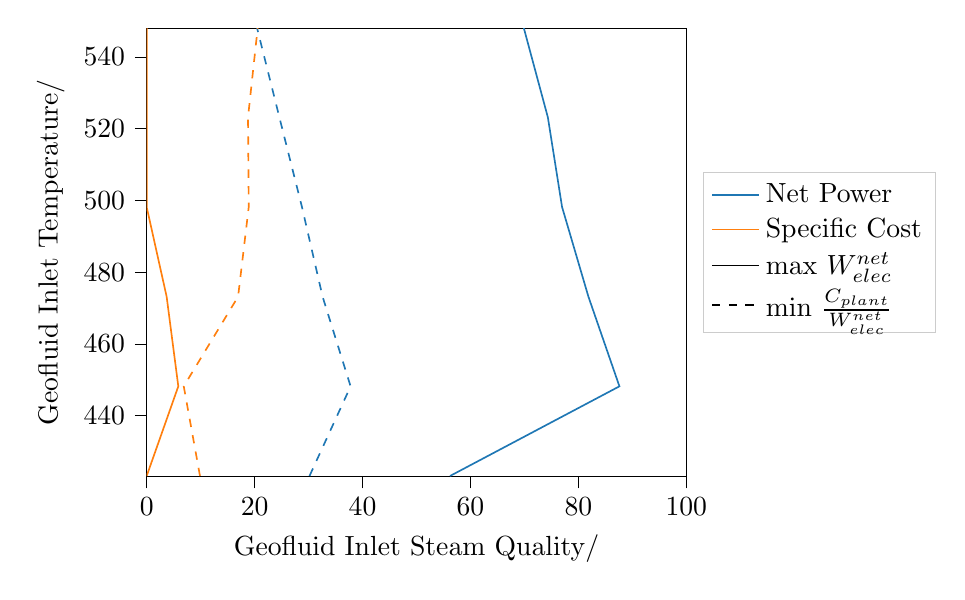
\begin{tikzpicture}

\definecolor{darkgray176}{RGB}{176,176,176}
\definecolor{darkorange25512714}{RGB}{255,127,14}
\definecolor{lightgray204}{RGB}{204,204,204}
\definecolor{steelblue31119180}{RGB}{31,119,180}

\begin{axis}[
legend cell align={left},
legend style={fill opacity=0.8, draw opacity=1, text opacity=1, draw=lightgray204, at={(1.03, 0.5)}, anchor=west},
tick align=outside,
tick pos=left,
x grid style={darkgray176},
xlabel={Geofluid Inlet Steam Quality/\unit{\percent}},
xmin=0, xmax=100,
xtick style={color=black},
y grid style={darkgray176},
ylabel={Geofluid Inlet Temperature/\unit{\K}},
ymin=423, ymax=548,
ytick style={color=black}
]
\addplot [semithick, steelblue31119180]
table {%
56.211897840536 423.15
87.6035000467854 448.15
81.8582827723205 473.15
76.9746128225413 498.15
74.343495146738 523.15
69.870082455215 548.15
};
\addlegendentry{Net Power}
\addplot [semithick, darkorange25512714]
table {%
0 423.15
5.86239070301085 448.15
3.70072396216428 473.15
0 498.15
0 523.15
0 548.15
};
\addlegendentry{Specific Cost}
\addplot [semithick, black]
table {%
0 -1
1 -1
};
\addlegendentry{max \(W_{elec}^{net}\)}
\addplot [semithick, black, dashed]
table {%
0 -1
1 -1
};
\addlegendentry{min \(\frac{C_{plant}}{W_{elec}^{net}}\)}
\addplot [semithick, steelblue31119180, dashed, forget plot]
table {%
30.1732199888322 423.15
37.7893009240293 448.15
32.5990272774492 473.15
28.7760448540457 498.15
24.595078256838 523.15
20.4394782095746 548.15
};
\addplot [semithick, darkorange25512714, dashed, forget plot]
table {%
9.88043234136831 423.15
6.87102869593706 448.15
16.9397882658249 473.15
18.9121530717588 498.15
18.7789988175102 523.15
20.5758201963607 548.15
};
\end{axis}

\end{tikzpicture}

    %     \caption{The geofluid inlet conditions for which the binary \ac{ORC} and single flash \ac{DSC} geothermal power plants deliver equal net electrical power or have equal specific plant costs. Left of the lines the binary \ac{ORC} outperforms the single flash \ac{DSC} plant. Solid lines indicate binary \ac{ORC}s with maximum net electrical power. Dashed lines indicate binary \ac{ORC}s with minimum specific cost.}
    %     \label{fig:prosim_purewater_Breakeven_DSC_vs_ORC}
    % \end{figure}

\subsection{Conclusions}
    Binary \ac{ORC}s can thermodynamically outperform \ac{DSC} geothermal power plants for a wide range of geofluid inlet conditions. However from a cost perspective, the application envelope of such thermodynamically optimised binary \ac{ORC}s is limited to low geofluid inlet vapour qualities.

    With the turbine and condenser being the main cost components, their size optimisation represents the largest potential for cost reductions. For instance, the size and cost of the condenser could be reduced by enforcing a larger approach temperature, at the expense of turbine power, or the use of a recuperator to improve the overall heat transfer coefficient for the cooling of the super-heating turbine outlet vapour (i.e. vapour-liquid contacting in the recuperator versus vapour-vapour contacting in the condenser).

\clearpage